% Options for packages loaded elsewhere
\PassOptionsToPackage{unicode}{hyperref}
\PassOptionsToPackage{hyphens}{url}
%
\documentclass[
]{book}
\usepackage{amsmath,amssymb}
\usepackage{lmodern}
\usepackage{iftex}
\ifPDFTeX
  \usepackage[T1]{fontenc}
  \usepackage[utf8]{inputenc}
  \usepackage{textcomp} % provide euro and other symbols
\else % if luatex or xetex
  \usepackage{unicode-math}
  \defaultfontfeatures{Scale=MatchLowercase}
  \defaultfontfeatures[\rmfamily]{Ligatures=TeX,Scale=1}
  \setmonofont[]{Lucida Console}
\fi
% Use upquote if available, for straight quotes in verbatim environments
\IfFileExists{upquote.sty}{\usepackage{upquote}}{}
\IfFileExists{microtype.sty}{% use microtype if available
  \usepackage[]{microtype}
  \UseMicrotypeSet[protrusion]{basicmath} % disable protrusion for tt fonts
}{}
\makeatletter
\@ifundefined{KOMAClassName}{% if non-KOMA class
  \IfFileExists{parskip.sty}{%
    \usepackage{parskip}
  }{% else
    \setlength{\parindent}{0pt}
    \setlength{\parskip}{6pt plus 2pt minus 1pt}}
}{% if KOMA class
  \KOMAoptions{parskip=half}}
\makeatother
\usepackage{xcolor}
\usepackage{color}
\usepackage{fancyvrb}
\newcommand{\VerbBar}{|}
\newcommand{\VERB}{\Verb[commandchars=\\\{\}]}
\DefineVerbatimEnvironment{Highlighting}{Verbatim}{commandchars=\\\{\}}
% Add ',fontsize=\small' for more characters per line
\usepackage{framed}
\definecolor{shadecolor}{RGB}{248,248,248}
\newenvironment{Shaded}{\begin{snugshade}}{\end{snugshade}}
\newcommand{\AlertTok}[1]{\textcolor[rgb]{0.94,0.16,0.16}{#1}}
\newcommand{\AnnotationTok}[1]{\textcolor[rgb]{0.56,0.35,0.01}{\textbf{\textit{#1}}}}
\newcommand{\AttributeTok}[1]{\textcolor[rgb]{0.77,0.63,0.00}{#1}}
\newcommand{\BaseNTok}[1]{\textcolor[rgb]{0.00,0.00,0.81}{#1}}
\newcommand{\BuiltInTok}[1]{#1}
\newcommand{\CharTok}[1]{\textcolor[rgb]{0.31,0.60,0.02}{#1}}
\newcommand{\CommentTok}[1]{\textcolor[rgb]{0.56,0.35,0.01}{\textit{#1}}}
\newcommand{\CommentVarTok}[1]{\textcolor[rgb]{0.56,0.35,0.01}{\textbf{\textit{#1}}}}
\newcommand{\ConstantTok}[1]{\textcolor[rgb]{0.00,0.00,0.00}{#1}}
\newcommand{\ControlFlowTok}[1]{\textcolor[rgb]{0.13,0.29,0.53}{\textbf{#1}}}
\newcommand{\DataTypeTok}[1]{\textcolor[rgb]{0.13,0.29,0.53}{#1}}
\newcommand{\DecValTok}[1]{\textcolor[rgb]{0.00,0.00,0.81}{#1}}
\newcommand{\DocumentationTok}[1]{\textcolor[rgb]{0.56,0.35,0.01}{\textbf{\textit{#1}}}}
\newcommand{\ErrorTok}[1]{\textcolor[rgb]{0.64,0.00,0.00}{\textbf{#1}}}
\newcommand{\ExtensionTok}[1]{#1}
\newcommand{\FloatTok}[1]{\textcolor[rgb]{0.00,0.00,0.81}{#1}}
\newcommand{\FunctionTok}[1]{\textcolor[rgb]{0.00,0.00,0.00}{#1}}
\newcommand{\ImportTok}[1]{#1}
\newcommand{\InformationTok}[1]{\textcolor[rgb]{0.56,0.35,0.01}{\textbf{\textit{#1}}}}
\newcommand{\KeywordTok}[1]{\textcolor[rgb]{0.13,0.29,0.53}{\textbf{#1}}}
\newcommand{\NormalTok}[1]{#1}
\newcommand{\OperatorTok}[1]{\textcolor[rgb]{0.81,0.36,0.00}{\textbf{#1}}}
\newcommand{\OtherTok}[1]{\textcolor[rgb]{0.56,0.35,0.01}{#1}}
\newcommand{\PreprocessorTok}[1]{\textcolor[rgb]{0.56,0.35,0.01}{\textit{#1}}}
\newcommand{\RegionMarkerTok}[1]{#1}
\newcommand{\SpecialCharTok}[1]{\textcolor[rgb]{0.00,0.00,0.00}{#1}}
\newcommand{\SpecialStringTok}[1]{\textcolor[rgb]{0.31,0.60,0.02}{#1}}
\newcommand{\StringTok}[1]{\textcolor[rgb]{0.31,0.60,0.02}{#1}}
\newcommand{\VariableTok}[1]{\textcolor[rgb]{0.00,0.00,0.00}{#1}}
\newcommand{\VerbatimStringTok}[1]{\textcolor[rgb]{0.31,0.60,0.02}{#1}}
\newcommand{\WarningTok}[1]{\textcolor[rgb]{0.56,0.35,0.01}{\textbf{\textit{#1}}}}
\usepackage{longtable,booktabs,array}
\usepackage{calc} % for calculating minipage widths
% Correct order of tables after \paragraph or \subparagraph
\usepackage{etoolbox}
\makeatletter
\patchcmd\longtable{\par}{\if@noskipsec\mbox{}\fi\par}{}{}
\makeatother
% Allow footnotes in longtable head/foot
\IfFileExists{footnotehyper.sty}{\usepackage{footnotehyper}}{\usepackage{footnote}}
\makesavenoteenv{longtable}
\usepackage{graphicx}
\makeatletter
\def\maxwidth{\ifdim\Gin@nat@width>\linewidth\linewidth\else\Gin@nat@width\fi}
\def\maxheight{\ifdim\Gin@nat@height>\textheight\textheight\else\Gin@nat@height\fi}
\makeatother
% Scale images if necessary, so that they will not overflow the page
% margins by default, and it is still possible to overwrite the defaults
% using explicit options in \includegraphics[width, height, ...]{}
\setkeys{Gin}{width=\maxwidth,height=\maxheight,keepaspectratio}
% Set default figure placement to htbp
\makeatletter
\def\fps@figure{htbp}
\makeatother
\setlength{\emergencystretch}{3em} % prevent overfull lines
\providecommand{\tightlist}{%
  \setlength{\itemsep}{0pt}\setlength{\parskip}{0pt}}
\setcounter{secnumdepth}{5}
\newlength{\cslhangindent}
\setlength{\cslhangindent}{1.5em}
\newlength{\csllabelwidth}
\setlength{\csllabelwidth}{3em}
\newlength{\cslentryspacingunit} % times entry-spacing
\setlength{\cslentryspacingunit}{\parskip}
\newenvironment{CSLReferences}[2] % #1 hanging-ident, #2 entry spacing
 {% don't indent paragraphs
  \setlength{\parindent}{0pt}
  % turn on hanging indent if param 1 is 1
  \ifodd #1
  \let\oldpar\par
  \def\par{\hangindent=\cslhangindent\oldpar}
  \fi
  % set entry spacing
  \setlength{\parskip}{#2\cslentryspacingunit}
 }%
 {}
\usepackage{calc}
\newcommand{\CSLBlock}[1]{#1\hfill\break}
\newcommand{\CSLLeftMargin}[1]{\parbox[t]{\csllabelwidth}{#1}}
\newcommand{\CSLRightInline}[1]{\parbox[t]{\linewidth - \csllabelwidth}{#1}\break}
\newcommand{\CSLIndent}[1]{\hspace{\cslhangindent}#1}
\usepackage{booktabs}
\usepackage{color}
\usepackage{xcolor}
\usepackage{framed}
\usepackage{tcolorbox}
\definecolor{lightgray}{gray}{0.90}

% \newenvironment{yourturn}{
%   \definecolor{lightgray}{gray}{0.90}  % black
%   \color{black}
%   \begin{shaded}}
%  {\end{shaded}}
%
%
\definecolor{lightgray}{gray}{0.90}
\newtcolorbox{yourturn}{
  colback=lightgray,
  colframe=black,
  coltext=black,
  boxsep=5pt,
  arc=4pt}
\usepackage{amsmath}
\usepackage{booktabs}
\usepackage{caption}
\usepackage{longtable}
\usepackage{array}
\usepackage{multirow}
\usepackage{wrapfig}
\usepackage{float}
\usepackage{colortbl}
\usepackage{pdflscape}
\usepackage{tabu}
\usepackage{threeparttable}
\usepackage{threeparttablex}
\usepackage[normalem]{ulem}
\usepackage{makecell}
\usepackage{xcolor}
\ifLuaTeX
  \usepackage{selnolig}  % disable illegal ligatures
\fi
\IfFileExists{bookmark.sty}{\usepackage{bookmark}}{\usepackage{hyperref}}
\IfFileExists{xurl.sty}{\usepackage{xurl}}{} % add URL line breaks if available
\urlstyle{same} % disable monospaced font for URLs
\hypersetup{
  pdftitle={A Progressive Introduction to Linear Models},
  pdfauthor={Joshua French},
  hidelinks,
  pdfcreator={LaTeX via pandoc}}

\title{A Progressive Introduction to Linear Models}
\author{Joshua French}
\date{}

\usepackage{amsthm}
\newtheorem{theorem}{Theorem}[chapter]
\newtheorem{lemma}{Lemma}[chapter]
\newtheorem{corollary}{Corollary}[chapter]
\newtheorem{proposition}{Proposition}[chapter]
\newtheorem{conjecture}{Conjecture}[chapter]
\theoremstyle{definition}
\newtheorem{definition}{Definition}[chapter]
\theoremstyle{definition}
\newtheorem{example}{Example}[chapter]
\theoremstyle{definition}
\newtheorem{exercise}{Exercise}[chapter]
\theoremstyle{definition}
\newtheorem{hypothesis}{Hypothesis}[chapter]
\theoremstyle{remark}
\newtheorem*{remark}{Remark}
\newtheorem*{solution}{Solution}
\begin{document}
\maketitle

{
\setcounter{tocdepth}{1}
\tableofcontents
}
\hypertarget{preliminaries}{%
\chapter*{Preliminaries}\label{preliminaries}}
\addcontentsline{toc}{chapter}{Preliminaries}

I designed this book to progressively introduce you to the analysis of data using linear models. My goal is to provide you with the skills needed to perform a linear regression analysis sooner rather than later. Some material that could be covered together (for example, all the different types of statistical tests and confidence intervals) has been broken into two sections: an early one to give you foundational knowledge about the topic and then later material to advance your understanding. Most of the detailed derivations have been placed in \textbf{Going Deeper} sections or in their own chapter, which can be skipped over to more quickly progress through the material if you do not want to focus as much on theory.

\textbf{Acknowledgments}

The \textbf{bookdown} package (\protect\hyperlink{ref-R-bookdown}{Xie 2023}) was used to generate this book. The \textbf{kableExtra} package (\protect\hyperlink{ref-R-kableExtra}{Zhu 2021}) was to format the tables. The writing of the book was partially supported by the Colorado Department of Higher Education as part of the proposal ``OER for the Creation of Interactive Computational Notebooks and a Computational Pathway in Mathematics and Statistics''.

\textbf{Creative Commons License Information}


\includegraphics[width=1.22in]{pictures/cc-by-nc}

A Progressive Introduction to Linear Models by Joshua French is licensed under a \href{https://creativecommons.org/licenses/by-nc/4.0/}{Creative Commons Attribution-NonCommercial 4.0 International License}.

\hypertarget{r-foundations}{%
\chapter{R Foundations}\label{r-foundations}}

Meaningful data analysis requires the use of computer software.

R statistical software is one of the most popular tools for data analysis in academia, industry, and government. In what follows, I will attempt to lay a foundation of basic knowledge and skills with R that you will need for data analysis. I make no attempt to be exhaustive, and many other important aspects of using R (like plotting) will be discussed later, as needed.

\hypertarget{setting-up-r-and-rstudio-desktop}{%
\section{Setting up R and RStudio Desktop}\label{setting-up-r-and-rstudio-desktop}}

\textbf{What is R?}

R is a programming language and environment designed for statistical computing. It was introduced by Robert Gentleman and Robert Ihaka in 1993 as a free implementation of the \emph{S} programming language developed at Bell Laboratories \href{https://www.r-project.org/about.html}{(https://www.r-project.org/about.html)}

Some important facts about R are that:

\begin{itemize}
\tightlist
\item
  R is free, open source, and runs on many different types of computers (Windows, Mac, Linux, and others).
\item
  R is an interactive programming language.

  \begin{itemize}
  \tightlist
  \item
    You type and run a command in the Console for immediate feedback, in contrast to a compiled programming language, which compiles a program that is then executed.
  \end{itemize}
\item
  R is highly extendable.

  \begin{itemize}
  \tightlist
  \item
    Many user-created packages are available to extend the functionality beyond what is installed by default.
  \item
    Users can write their own functions and easily add software libraries to R.
  \end{itemize}
\end{itemize}

\textbf{Installing R}

To install R on your personal computer, you will need to download an installer program from the R Project's website \href{https://www.r-project.org/}{(https://www.r-project.org/)}. Links to download the installer program for your operating system \emph{should} be found at \url{https://cloud.r-project.org/}. Click on the download link appropriate for your computer's operating system and install R on your computer. If you have a Windows computer, a stable link for the most current installer program is available at \url{https://cloud.r-project.org/bin/windows/base/release.html}. (Similar links are not currently available for Mac and Linux computers.)

\textbf{Installing RStudio}

RStudio Desktop is a free ``front end'' for R provided by Posit Software (\url{https://posit.co/}). RStudio Desktop makes doing data analysis with R much easier by adding an Integrated Development Environment (IDE) and providing many other features. Currently, you may download RStudio at \url{https://posit.co/download/rstudio-desktop/}. You may need to navigate the RStudio website directly if this link no longer functions. Download the Free version of RStudio Desktop appropriate for your computer and install it.

Having installed both R and RStudio Desktop, you will want to open RStudio Desktop as you continue to learn about R.

\textbf{RStudio Layout}

RStudio Desktop has four panes:

\begin{enumerate}
\def\labelenumi{\arabic{enumi}.}
\tightlist
\item
  Console: the pane where commands are run.
\item
  Source: the pane where you prepare commands to be run.
\item
  Environment/History: the pane where you can see all the objects in your workspace, your command history, and other information.
\item
  The Files/Plot/Packages/Help: the pane where you navigate between directories, where plots can be viewed, where you can see the packages available to be loaded, and where you can get help.
\end{enumerate}

To see all RStudio panes, press the keys \texttt{Ctrl\ +\ Alt\ +\ Shift\ +\ 0} on a PC or \texttt{Cmd\ +\ Option\ +\ Shift\ +\ 0} on a Mac.

Figure \ref{fig:rstudiopanes} displays a labeled graphic of the panes. Your panes are likely in a different order than the graphic shown because I have customized my workspace for my own needs.

\begin{figure}
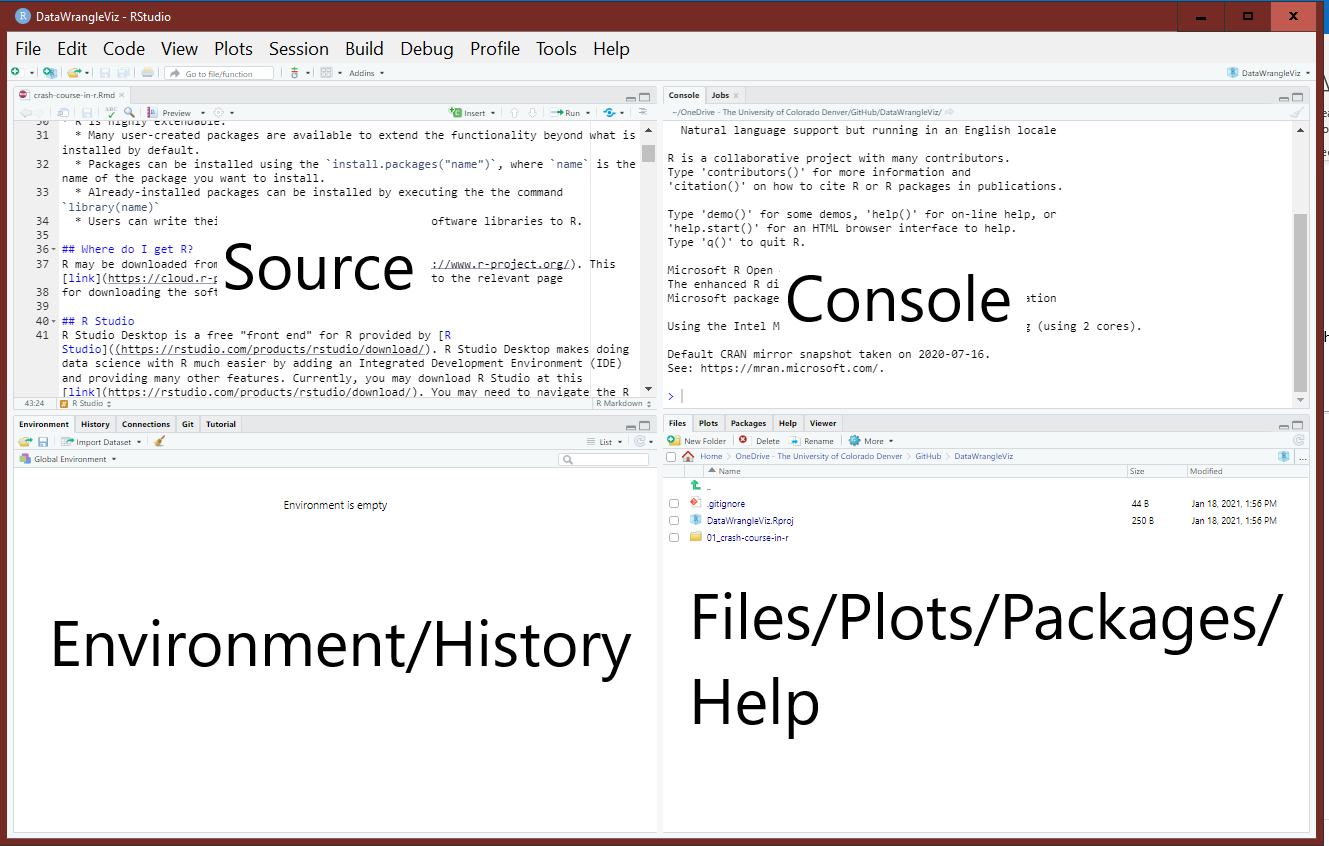
\includegraphics[width=0.9\linewidth]{pictures/rstudio_panes} \caption{The RStudio panes labeled for convenience.}\label{fig:rstudiopanes}
\end{figure}

\textbf{Customizing the RStudio workspace}

At this point, I would highly encourage you to make one small workspace customization that will likely save you from experiencing future frustration. R provides a ``feature'' of that allows you to ``save a workspace''. This allows you to easily pick up where you left off your last analysis. The issue with this is that over time you accumulate a lot of environmental artifacts that can conflict with each other. This can lead to errors and incorrect results that you will need to deal with. Additionally, this ``feature'' hinders the ability of others to reproduce your analysis because other users are unlikely to have the same workspace.

To turn off this feature, in the RStudio menu bar click Tools → Global Options and then make sure the ``General'' option is selected. Then make the following changes (if necessary):

\begin{enumerate}
\def\labelenumi{\arabic{enumi}.}
\tightlist
\item
  Uncheck the box for ``Restore .RData into workspace at startup''.
\item
  Change the toggle box for ``Save workspace to .RData on exit'' to ``Never''.
\item
  Click Apply then OK to save the changes.
\end{enumerate}

Figure \ref{fig:generaloptions} displays what these options should look like.

\begin{figure}
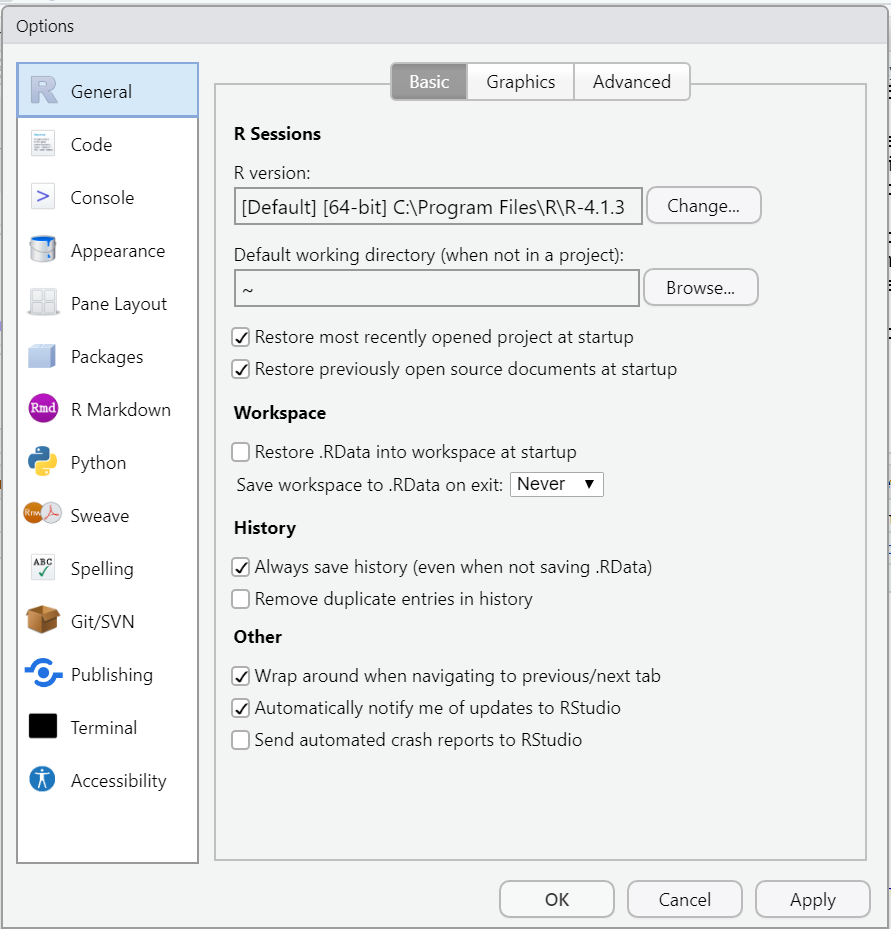
\includegraphics[width=0.9\linewidth]{pictures/general_options} \caption{The General options window.}\label{fig:generaloptions}
\end{figure}

\hypertarget{running-code-scripts-and-comments}{%
\section{Running code, scripts, and comments}\label{running-code-scripts-and-comments}}

You can run code in R by typing it in the Console next to the \texttt{\textgreater{}} symbol and pressing the Enter key.

If you need to successively run multiple commands, it's better to write your commands in a ``script'' file and then save the file. The commands in a Script file are often generically referred to as ``code''.

Script files make it easy to:

\begin{itemize}
\tightlist
\item
  Reproduce your data analysis without retyping all your commands.
\item
  Share your code with others.
\end{itemize}

A new Script file can be obtained by:

\begin{itemize}
\tightlist
\item
  Clicking File → New File → R Script in the RStudio menu bar.
\item
  Pressing \texttt{Ctrl\ +\ Shift\ +\ n} on a PC or \texttt{Cmd\ +\ Shift\ +\ n} on a Mac.
\end{itemize}

There are various ways to run code from a Script file. The most common ones are:

\begin{enumerate}
\def\labelenumi{\arabic{enumi}.}
\tightlist
\item
  Highlight the code you want to run and click the Run button
  
\includegraphics[width=1.35in]{pictures/run_button} at the top of the Script pane.
\item
  Highlight the code you want to run and press ``Ctrl + Enter'' on your keyboard. If you don't highlight anything, by default, RStudio runs the command the cursor currently lies on.
\end{enumerate}

To save a Script file:

\begin{itemize}
\tightlist
\item
  Click File → Save in the RStudio menu bar.
\item
  Press \texttt{Ctrl\ +\ s} on a PC or \texttt{Cmd\ +\ s} on a Mac.
\end{itemize}

A comment is a set of text ignored by R when submitted to the Console.

A comment is indicated by the \texttt{\#} symbol. Nothing to the right of the \texttt{\#} is executed by the Console.

To comment (or uncomment) multiple lines of code in the Source pane of RStudio, highlight the code you want to comment and press \texttt{Ctrl\ +\ Shift\ +\ c} on a PC or \texttt{Cmd\ +\ Shift\ +\ c} on a Mac.

\begin{yourturn}

\textbf{Your turn}

Perform the following tasks:

\begin{enumerate}
\def\labelenumi{\arabic{enumi}.}
\tightlist
\item
  Type \texttt{1+1} in the Console and press Enter.
\item
  Open a new Script in RStudio.
\item
  Type \texttt{mean(1:3)} in your Script file.
\item
  Type \texttt{\#\ mean(1:3)} in your Script file.
\item
  Run the commands from the Script using an approach mentioned above.
\item
  Save your Script file.
\item
  Use the keyboard shortcut to ``comment out'' some of the lines of your Script file.
\end{enumerate}

\end{yourturn}

\hypertarget{assignment}{%
\section{Assignment}\label{assignment}}

R works on various types of objects that we'll learn more about later.

To store an object in the computer's memory we must assign it a name using the assignment operator \texttt{\textless{}-} or the equal sign \texttt{=}.

Some comments:

\begin{itemize}
\tightlist
\item
  In general, both \texttt{\textless{}-} and \texttt{=} can be used for assignment.
\item
  Pressing \texttt{Alt\ +\ -} on a PC or \texttt{Option\ +\ -} on a Mac will insert \texttt{\textless{}-} into the R Console and Script files.

  \begin{itemize}
  \tightlist
  \item
    If you are creating an R Markdown file, then this shortcut will only insert \texttt{\textless{}-} if you are in an R code block.
  \end{itemize}
\item
  \texttt{\textless{}-} and \texttt{=} are NOT synonyms, but can be used identically most of the time.
\end{itemize}

\textbf{It is best to use \texttt{\textless{}-} for assigning a name to an object and reserving \texttt{=} for specifying function arguments.} See Section \ref{comparing-assignment-operators} for an explanation.

Once an object has been assigned a name, it can be printed by running the name of the object in the Console or using the \texttt{print} function.

\begin{yourturn}
\textbf{Your turn}

Run the following commands in the Console:

\begin{Shaded}
\begin{Highlighting}[]
\CommentTok{\# compute the mean of 1, 2, ..., 10 and assign the name m}
\NormalTok{m }\OtherTok{\textless{}{-}} \FunctionTok{mean}\NormalTok{(}\DecValTok{1}\SpecialCharTok{:}\DecValTok{10}\NormalTok{) }
\NormalTok{m }\CommentTok{\# print m}
\FunctionTok{print}\NormalTok{(m) }\CommentTok{\# print m a different way}
\end{Highlighting}
\end{Shaded}

After the comment, we compute the sample mean of the values \(1, 2, \ldots, 10\), then assign it the name \texttt{m}. The next two lines are different mechanisms for printing the information contained in the object \texttt{m} (which is just the number 5.5).

\end{yourturn}

\hypertarget{functions}{%
\section{Functions}\label{functions}}

A function is an object that performs a certain action or set of actions based on objects it receives from its arguments. We use a sequence of function calls to perform data analysis.

To use a function, you type the function's name in the Console (or Script) and then supply the function's ``arguments'' between parentheses, \texttt{()}.

The arguments of a function are pieces of data or information the function needs to perform the requested task (i.e., the function ``inputs''). Each argument you supply is separated by a comma, \texttt{,}. Some functions have default values for certain arguments and do not need to specified unless something beside the default behavior is desired.

e.g., the \texttt{mean} function computes the sample mean of an R object \texttt{x}. (How do I know? Because I looked at the documentation for the function by running \texttt{?mean} in the Console. We'll talk more about getting help with R shortly.) The \texttt{mean} function also has a \texttt{trim} argument that indicates the, ``\ldots{} fraction \ldots{} of observations to be trimmed from each end of \texttt{x} before the mean is computed'' (R Core Team (\protect\hyperlink{ref-R-base}{2023}), \texttt{?mean}).

Consider the examples below, in which we compute the mean of the set of values \texttt{1,\ 5,\ 3,\ 2,\ 10}.

\begin{Shaded}
\begin{Highlighting}[]
\FunctionTok{mean}\NormalTok{(}\FunctionTok{c}\NormalTok{(}\DecValTok{1}\NormalTok{, }\DecValTok{5}\NormalTok{, }\DecValTok{3}\NormalTok{, }\DecValTok{4}\NormalTok{, }\DecValTok{10}\NormalTok{))}
\DocumentationTok{\#\# [1] 4.6}
\FunctionTok{mean}\NormalTok{(}\FunctionTok{c}\NormalTok{(}\DecValTok{1}\NormalTok{, }\DecValTok{5}\NormalTok{, }\DecValTok{3}\NormalTok{, }\DecValTok{4}\NormalTok{, }\DecValTok{10}\NormalTok{), }\AttributeTok{trim =} \FloatTok{0.2}\NormalTok{)}
\DocumentationTok{\#\# [1] 4}
\end{Highlighting}
\end{Shaded}

The output differs for the two function calls because in the first we compute \texttt{(1\ +\ 5\ +\ 3\ +\ 4\ +\ 10)/5\ =\ 23/5\ =\ 4.6} while in the second we remove the first 20\% and last 20\% of the values (i.e., dropping \texttt{1} and \texttt{10}) and compute \texttt{(5\ +\ 3\ +\ 4)/3\ =\ 12/3\ =\ 4}.

\hypertarget{packages}{%
\section{Packages}\label{packages}}

Packages are collections of functions, data, and other objects that extend the functionality available in R by default.

R packages can be installed using the \texttt{install.packages} function and loaded using the \texttt{library} function.

\begin{yourturn}

\textbf{Your turn}

The \textbf{tidyverse} (\url{https://www.tidyverse.org}, Wickham (\protect\hyperlink{ref-R-tidyverse}{2023b})) is a popular ecosystem of R packages used for manipulating, tidying, and plotting data. Currently, the \textbf{tidyverse} is comprised of the following packages:

\begin{itemize}
\tightlist
\item
  \textbf{ggplot2}: A package for plotting based on the ``Grammar of Graphics'' (\protect\hyperlink{ref-R-ggplot2}{Wickham, Chang, et al. 2023}).
\item
  \textbf{purrr}: A package for functional programming (\protect\hyperlink{ref-R-purrr}{Wickham and Henry 2023}).
\item
  \textbf{tibble}: A package providing a more advanced data frame (\protect\hyperlink{ref-R-tibble}{Müller and Wickham 2023}).
\item
  \textbf{dplyr}: A package for manipulating data. More specifically, it provides '' a grammar of data manipulation'' (\protect\hyperlink{ref-R-dplyr}{Wickham, François, et al. 2023}).
\item
  \textbf{tidyr}: A package to help create ``tidy'' data (\protect\hyperlink{ref-R-tidyr}{Wickham, Vaughan, and Girlich 2023}). Tidy data is an data organization style often convenient for data analysis.
\item
  \textbf{stringr}: A package for working with character/string data (\protect\hyperlink{ref-R-stringr}{Wickham 2022a}).
\item
  \textbf{readr}: A package for importing data (\protect\hyperlink{ref-R-readr}{Wickham, Hester, and Bryan 2023}).
\item
  \textbf{forcats}: A package for working with categorical data (\protect\hyperlink{ref-R-forcats}{Wickham 2023a}).
\end{itemize}

Install the set of \textbf{tidyverse} R packages by running the command below in the Console.

\begin{Shaded}
\begin{Highlighting}[]
\FunctionTok{install.packages}\NormalTok{(}\StringTok{"tidyverse"}\NormalTok{)}
\end{Highlighting}
\end{Shaded}

After you install \textbf{tidyverse}, load the package(s) by running the command below.

\begin{Shaded}
\begin{Highlighting}[]
\FunctionTok{library}\NormalTok{(tidyverse)}
\end{Highlighting}
\end{Shaded}

You should see something like the following output:

\begin{verbatim}
## -- Attaching core tidyverse packages ------------------------ tidyverse 2.0.0 --
## v dplyr     1.1.0     v readr     2.1.4
## v forcats   1.0.0     v stringr   1.5.0
## v ggplot2   3.4.1     v tibble    3.2.0
## v lubridate 1.9.2     v tidyr     1.3.0
## v purrr     1.0.1     
## -- Conflicts ------------------------------------------ tidyverse_conflicts() --
## x dplyr::filter() masks stats::filter()
## x dplyr::lag()    masks stats::lag()
## i Use the ]8;;http://conflicted.r-lib.org/conflicted package]8;; to force all conflicts to become errors
\end{verbatim}

\end{yourturn}

Different packages may use the same function name to provide certain functionality. The functions will likely be used for different tasks or require different arguments. E.g., You may have noticed when you loaded the \textbf{tidyverse} above that \texttt{dplyr::lag()} masks \texttt{stats::lag()}. What this means is that both the \textbf{dplyr} and \textbf{stats} packages have a function called \texttt{lag}.

To refer to a function in a specific package, we should add \texttt{package::} prior to the function name. In the code below, we run \texttt{stats::lag} and \texttt{dplyr::lag} on two different objects using the \texttt{::} syntax.

\begin{Shaded}
\begin{Highlighting}[]
\NormalTok{stats}\SpecialCharTok{::}\FunctionTok{lag}\NormalTok{(}\DecValTok{1}\SpecialCharTok{:}\DecValTok{10}\NormalTok{, }\DecValTok{2}\NormalTok{)}
\DocumentationTok{\#\#  [1]  1  2  3  4  5  6  7  8  9 10}
\DocumentationTok{\#\# attr(,"tsp")}
\DocumentationTok{\#\# [1] {-}1  8  1}
\NormalTok{dplyr}\SpecialCharTok{::}\FunctionTok{lag}\NormalTok{(}\DecValTok{1}\SpecialCharTok{:}\DecValTok{10}\NormalTok{, }\DecValTok{2}\NormalTok{)}
\DocumentationTok{\#\#  [1] NA NA  1  2  3  4  5  6  7  8}
\end{Highlighting}
\end{Shaded}

The output returned by the two functions is different because the functions are intended to do different things. The \texttt{stats::lag} function call shifts the time base of the provided time series object back 2 units, while the call to \texttt{dplyr::lag} provides the values 2 positions earlier in the object. Note: you don't need to understand the \texttt{lag} function in the example above. The example is provided to demonstrate how to use the \texttt{::} syntax to call to a function in a specific package when the function name has conflicts in multiple packages.

\hypertarget{getting-help}{%
\section{Getting help}\label{getting-help}}

There are many ways to get help in R.

If you know the command for which you want help, then run \texttt{?command} (where command is replaced the name of the relevant command) in the Console, to access the documentation for the object. This approach will also work with data sets, package names, object classes, etc. If you need to refer to a function in a specific package, you can use \texttt{?package::function} to get help on a specific function, e.g., \texttt{?dplyr::filter}.

The documentation will provide:

\begin{itemize}
\tightlist
\item
  A \textbf{Description} section with general information about the function or object.
\item
  A **Usage* section with a generic template for using the function or object.
\item
  An \textbf{Arguments} section summarizing the function inputs the function needs.
\item
  A \textbf{Details} section may be provided with additional information about how the function or object.
\item
  A \textbf{Value} section that describes what is returned by the function.
\item
  A \textbf{Examples} section providing examples of how to use the function. Usually, these can be copied and pasted into the Console to better understand the function arguments and what it produced.
\end{itemize}

If you need to find a command to help you with a certain \emph{topic}, then \texttt{??topic} will search for the topic through all installed documentation and bring up any vignettes, code demonstrations, or help pages that include the topic for which you searched.

If you are trying to figure out why an error is being produced, what packages can be used to perform a certain analysis, how to perform a complex task that you can't seem to figure out, etc., then simply do a web search for what you're trying to figure out! Because R is such a popular programming language, it is likely you will find a \href{https://www.stackoverflow.com}{stackoverflow} response, a helpful blog post, an R users forum response, etc., that at least partially addresses your question.

\begin{yourturn}

Do the following:

\begin{enumerate}
\def\labelenumi{\arabic{enumi}.}
\tightlist
\item
  Run\texttt{?lm} in the Console to get help on the \texttt{lm} function, which is one of the main functions used for fitting linear models.
\item
  Run \texttt{??logarithms} in the Console to search the R documentation for information about logarithms. It is likely that you will see multiple Help pages that mention ``logarithm'', so you may end up needing to find the desired entry via trial and error.
\item
  Run a web search for something along the lines of ``How do I change the size of the axis labels in an R plot?''.
\end{enumerate}

\end{yourturn}

\hypertarget{data-types-and-structures}{%
\section{Data types and structures}\label{data-types-and-structures}}

\hypertarget{basic-data-types}{%
\subsection{Basic data types}\label{basic-data-types}}

R has 6 basic (``atomic'') vector types \href{https://cran.r-project.org/doc/manuals/r-release/R-lang.html\#Basic-types}{(https://cran.r-project.org/doc/manuals/r-release/R-lang.html\#Basic-types)} (\protect\hyperlink{ref-R-base}{R Core Team 2023}):

\begin{enumerate}
\def\labelenumi{\arabic{enumi}.}
\tightlist
\item
  character: collections of characters. E.g., \texttt{"a"}, \texttt{"hello\ world!"}.
\item
  double: decimal numbers. e.g., \texttt{1.2}, \texttt{1.0}.
\item
  integer: whole numbers. In R, you must add \texttt{L} to the end of a number to specify it as an integer. E.g., \texttt{1L} is an integer but \texttt{1} is a double.
\item
  logical: boolean values, \texttt{TRUE} and \texttt{FALSE}.
\item
  complex: complex numbers. E.g., \texttt{1+3i}.
\item
  raw: a type to hold raw bytes.
\end{enumerate}

Both double and integer values are specific types of numeric values.

The \texttt{typeof} function returns the R internal type or storage mode of any object.

Consider the following commands and output:

\begin{Shaded}
\begin{Highlighting}[]
\CommentTok{\# determine basic data type}
\FunctionTok{typeof}\NormalTok{(}\DecValTok{1}\NormalTok{)}
\DocumentationTok{\#\# [1] "double"}
\FunctionTok{typeof}\NormalTok{(1L)}
\DocumentationTok{\#\# [1] "integer"}
\FunctionTok{typeof}\NormalTok{(}\StringTok{"hello world!"}\NormalTok{)}
\DocumentationTok{\#\# [1] "character"}
\end{Highlighting}
\end{Shaded}

\hypertarget{other-important-object-types}{%
\subsection{Other important object types}\label{other-important-object-types}}

There are other important types of objects in R that are not basic. We will discuss a few. The R Project manual provides additional information about available types \href{https://cran.r-project.org/doc/manuals/r-release/R-lang.html\#Basic-types}{(https://cran.r-project.org/doc/manuals/r-release/R-lang.html\#Basic-types)}.

\hypertarget{numeric}{%
\subsubsection{Numeric}\label{numeric}}

An object is \texttt{numeric} if it is of type \texttt{integer} or \texttt{double}. In that case, it's \texttt{mode} is said to be \texttt{numeric}.

The \texttt{is.numeric} function tests whether an object can be interpreted as numbers. We can use it to determine whether an object is \texttt{numeric}, as in the code run below.

\begin{Shaded}
\begin{Highlighting}[]
\CommentTok{\# is the object numeric?}
\FunctionTok{is.numeric}\NormalTok{(}\StringTok{"hello world!"}\NormalTok{)}
\DocumentationTok{\#\# [1] FALSE}
\FunctionTok{is.numeric}\NormalTok{(}\DecValTok{1}\NormalTok{)}
\DocumentationTok{\#\# [1] TRUE}
\FunctionTok{is.numeric}\NormalTok{(1L)}
\DocumentationTok{\#\# [1] TRUE}
\end{Highlighting}
\end{Shaded}

\hypertarget{null}{%
\subsubsection{NULL}\label{null}}

\texttt{NULL} is a special object to indicate an object is absent. An object having a length of zero is not the same thing as an object being absent.

\hypertarget{na}{%
\subsubsection{NA}\label{na}}

A ``missing value'' occurs when the value of something isn't known. R uses the special object \texttt{NA} to represent a missing value.

If you have a missing value, you should represent that value as \texttt{NA}. Note: \texttt{"NA"} is not the same thing as \texttt{NA}.

\hypertarget{functions-1}{%
\subsubsection{Functions}\label{functions-1}}

From R's perspective, a function is simply another data type.

\hypertarget{a-comment-about-classes}{%
\subsubsection{A comment about classes}\label{a-comment-about-classes}}

Every R object has a \texttt{class} that may be distinct from its type. Many functions will operate differently depending on an object's \texttt{class}.

\hypertarget{data-structures}{%
\subsection{Data structures}\label{data-structures}}

R operates on data structures. A data structure is a ``container'' that holds certain kinds of information.

R has 5 basic data structures:

\begin{enumerate}
\def\labelenumi{\arabic{enumi}.}
\tightlist
\item
  vector.
\item
  matrix.
\item
  array.
\item
  data frame.
\item
  list.
\end{enumerate}

Vectors, matrices, and arrays are homogeneous objects that can only store a single data type at a time. Data frames and lists can store multiple data types.

Vectors and lists are considered one-dimensional objects. A list is technically a vector. Vectors of a single type are atomic vectors \href{https://cran.r-project.org/doc/manuals/r-release/R-lang.html\#List-objects}{(https://cran.r-project.org/doc/manuals/r-release/R-lang.html\#List-objects)}. Matrices and data frames are considered two-dimensional objects. Arrays can have 1 or more dimensions.

The relationship between dimensionality and data type for the basic data structures is summarized in Table \ref{tab:datastructures2}, which is based on a \href{https://adv-r.had.co.nz/Data-structures.html\#data-structure}{table} in the first edition of Hadley Wickham's \emph{Advanced R} \href{https://adv-r.had.co.nz/Data-structures.html\#data-structure}{(https://adv-r.had.co.nz/Data-structures.html\#data-structure)}.

\begin{longtable}{l|ll}
\toprule
\multicolumn{1}{l}{} & \multicolumn{2}{c}{data type} \\ 
\cmidrule(lr){2-3}
\multicolumn{1}{l}{\# of dimensions} & homogeneous & heterogeneous \\ 
\midrule
1 & atomic vector & list \\ 
2 & matrix & data frame \\ 
1 or more & array &  \\ 
\bottomrule
\end{longtable}

\hypertarget{vectors}{%
\section{Vectors}\label{vectors}}

A \emph{vector} is a one-dimensional set of data of the same type.

\hypertarget{creation}{%
\subsection{Creation}\label{creation}}

The most basic way to create a vector is the \texttt{c} (combine) function. The \texttt{c} function combines values into an atomic vector or list.

The following commands create vectors of type \texttt{numeric}, \texttt{character}, and \texttt{logical}, respectively.

\begin{itemize}
\tightlist
\item
  \texttt{c(1,\ 2,\ 5.3,\ 6,\ -2,\ 4)}
\item
  \texttt{c("one",\ "two",\ "three")}
\item
  \texttt{c(TRUE,\ TRUE,\ FALSE,\ TRUE)}
\end{itemize}

R provides two main functions for creating vectors with specific patterns: \texttt{seq} and \texttt{rep}.

The \texttt{seq} (sequence) function is used to create an equidistant series of numeric values. Some examples:

\begin{itemize}
\tightlist
\item
  \texttt{seq(1,\ 10)} creates a sequence of numbers from 1 to 10 in increments of 1.
\item
  \texttt{1:10} creates a sequence of numbers from 1 to 10 in increments of 1.
\item
  \texttt{seq(1,\ 20,\ by\ =\ 2)} creates a sequence of numbers from 1 to 20 in increments of 2.
\item
  \texttt{seq(10,\ 20,\ len\ =\ 100)} creates a sequence of numbers from 10 to 20 of length 100.
\end{itemize}

The \texttt{rep} (replicate) function can be used to create a vector by replicating values. Some examples:

\begin{itemize}
\tightlist
\item
  \texttt{rep(1:3,\ times\ =\ 3)} replicates the sequence \texttt{1,\ 2,\ 3} three times in a row.
\item
  \texttt{rep(c("trt1",\ "trt2",\ "trt3"),\ times\ =\ 1:3)} replicates \texttt{"trt1"} once, \texttt{"trt2"} twice, and \texttt{"trt3"} three times.
\item
  \texttt{rep(1:3,\ each\ =\ 3)} replicates each element of the sequence 1, 2, 3 three times.
\end{itemize}

Multiple vectors can be combined into a new vector object using the \texttt{c} function. E.g., \texttt{c(v1,\ v2,\ v3)} would combine vectors \texttt{v1}, \texttt{v2}, and \texttt{v3}.

\begin{yourturn}

\textbf{Your turn}

Run the commands below in the Console to see what is printed. After you do that, try to answer the following questions:

\begin{itemize}
\tightlist
\item
  What does the \texttt{by} argument of the \texttt{seq} function control?
\item
  What does the \texttt{len} argument of the \texttt{seq} function control?
\item
  What does the \texttt{times} argument of the \texttt{rep} function control?
\item
  What does the \texttt{each} argument of the \texttt{rep} function control?
\end{itemize}

\begin{Shaded}
\begin{Highlighting}[]
\CommentTok{\# vector creation}
\FunctionTok{c}\NormalTok{(}\DecValTok{1}\NormalTok{, }\DecValTok{2}\NormalTok{, }\FloatTok{5.3}\NormalTok{, }\DecValTok{6}\NormalTok{, }\SpecialCharTok{{-}}\DecValTok{2}\NormalTok{, }\DecValTok{4}\NormalTok{)}
\FunctionTok{c}\NormalTok{(}\StringTok{"one"}\NormalTok{, }\StringTok{"two"}\NormalTok{, }\StringTok{"three"}\NormalTok{)}
\FunctionTok{c}\NormalTok{(}\ConstantTok{TRUE}\NormalTok{, }\ConstantTok{TRUE}\NormalTok{, }\ConstantTok{FALSE}\NormalTok{, }\ConstantTok{TRUE}\NormalTok{)}
\CommentTok{\# sequences of values}
\FunctionTok{seq}\NormalTok{(}\DecValTok{1}\NormalTok{, }\DecValTok{10}\NormalTok{)}
\DecValTok{1}\SpecialCharTok{:}\DecValTok{10}
\FunctionTok{seq}\NormalTok{(}\DecValTok{1}\NormalTok{, }\DecValTok{20}\NormalTok{, }\AttributeTok{by =} \DecValTok{2}\NormalTok{)}
\FunctionTok{seq}\NormalTok{(}\DecValTok{10}\NormalTok{, }\DecValTok{20}\NormalTok{, }\AttributeTok{len =} \DecValTok{100}\NormalTok{)}
\CommentTok{\# replicated values}
\FunctionTok{rep}\NormalTok{(}\DecValTok{1}\SpecialCharTok{:}\DecValTok{3}\NormalTok{, }\AttributeTok{times =} \DecValTok{3}\NormalTok{)}
\FunctionTok{rep}\NormalTok{(}\FunctionTok{c}\NormalTok{(}\StringTok{"trt1"}\NormalTok{, }\StringTok{"trt2"}\NormalTok{, }\StringTok{"trt3"}\NormalTok{), }\AttributeTok{times =} \DecValTok{1}\SpecialCharTok{:}\DecValTok{3}\NormalTok{)}
\FunctionTok{rep}\NormalTok{(}\DecValTok{1}\SpecialCharTok{:}\DecValTok{3}\NormalTok{, }\AttributeTok{each =} \DecValTok{3}\NormalTok{)}
\end{Highlighting}
\end{Shaded}

Next, we can practice combining multiple vectors using \texttt{c}. Run the commands below in the Console.

\begin{Shaded}
\begin{Highlighting}[]
\NormalTok{v1 }\OtherTok{\textless{}{-}} \DecValTok{1}\SpecialCharTok{:}\DecValTok{5} \CommentTok{\# create a vector, v1}
\NormalTok{v2 }\OtherTok{\textless{}{-}} \FunctionTok{c}\NormalTok{(}\DecValTok{1}\NormalTok{, }\DecValTok{10}\NormalTok{, }\DecValTok{11}\NormalTok{) }\CommentTok{\# create another vector, v2}
\NormalTok{v3 }\OtherTok{\textless{}{-}} \FunctionTok{rep}\NormalTok{(}\DecValTok{1}\SpecialCharTok{:}\DecValTok{2}\NormalTok{, }\AttributeTok{each =} \DecValTok{3}\NormalTok{) }\CommentTok{\# crate a third vector, v3}
\NormalTok{new }\OtherTok{\textless{}{-}} \FunctionTok{c}\NormalTok{(v1, v2, v3) }\CommentTok{\# combine v1, v2, and v3 into a new vector}
\NormalTok{new }\CommentTok{\# print the combined vector}
\end{Highlighting}
\end{Shaded}

\end{yourturn}

\hypertarget{categorical-vectors}{%
\subsection{Categorical vectors}\label{categorical-vectors}}

Categorical data should be stored as a \texttt{factor} in R. Even though your code related to categorical data may work when stored as \texttt{character} or \texttt{numeric} data because a cautious developer planned for that possibility, it is best to use good coding practices that minimize potential issues.

The \texttt{factor} function takes a vector of values that can be coerced to type \texttt{character} and converts them to an object of class \texttt{factor}. In the code chunk below, we create two \texttt{factor} objects from vectors.

\begin{Shaded}
\begin{Highlighting}[]
\CommentTok{\# create some factor variables}
\NormalTok{f1 }\OtherTok{\textless{}{-}} \FunctionTok{factor}\NormalTok{(}\FunctionTok{rep}\NormalTok{(}\DecValTok{1}\SpecialCharTok{:}\DecValTok{6}\NormalTok{, }\AttributeTok{times =} \DecValTok{3}\NormalTok{))}
\NormalTok{f1}
\DocumentationTok{\#\#  [1] 1 2 3 4 5 6 1 2 3 4 5 6 1 2 3 4 5 6}
\DocumentationTok{\#\# Levels: 1 2 3 4 5 6}
\NormalTok{f2 }\OtherTok{\textless{}{-}} \FunctionTok{factor}\NormalTok{(}\FunctionTok{c}\NormalTok{(}\StringTok{"a"}\NormalTok{, }\DecValTok{7}\NormalTok{, }\StringTok{"blue"}\NormalTok{, }\StringTok{"blue"}\NormalTok{, }\ConstantTok{FALSE}\NormalTok{))}
\NormalTok{f2}
\DocumentationTok{\#\# [1] a     7     blue  blue  FALSE}
\DocumentationTok{\#\# Levels: 7 a blue FALSE}
\end{Highlighting}
\end{Shaded}

Note that when a \texttt{factor} object is printed that it lists the \texttt{Levels} (i.e., unique categories) of the object.

Some additional comments:

\begin{itemize}
\tightlist
\item
  \texttt{factor} objects aren't technically vectors (e.g., running \texttt{is.factor(f2)} based on the above code will return \texttt{FALSE}) though they essentially behave like vectors, which is why they are included here.
\item
  The \texttt{is.factor} function can be used to determine whether an object is a \texttt{factor}.
\item
  You can create \texttt{factor} objects with specific orderings of categories using the \texttt{level} and \texttt{ordered} arguments of the \texttt{factor} function (see \texttt{?factor} for more details).
\end{itemize}

\begin{yourturn}

\textbf{Your turn}

Attempt to complete the following tasks:

\begin{enumerate}
\def\labelenumi{\arabic{enumi}.}
\tightlist
\item
  Create a vector named \texttt{grp} that has two levels: \texttt{a} and \texttt{b}, where the first 7 values are \texttt{a} and the second 4 values are \texttt{b}.
\item
  Run \texttt{is.factor(grp)} in the Console.
\item
  Run \texttt{is.vector(grp)} in the Console.
\item
  Run \texttt{typeof(grp)} in the Console.
\end{enumerate}

Related to the last task, a \texttt{factor} object is \emph{technically} a collection of integers that have labels associated with each unique integer value.

Let's look at creating ordered \texttt{factor} objects. Suppose we have categorical data with the categories \texttt{small}, \texttt{medium}, and \texttt{large}. We create a \texttt{size} vector with hypothetical data below.

\begin{Shaded}
\begin{Highlighting}[]
\NormalTok{size }\OtherTok{\textless{}{-}} \FunctionTok{c}\NormalTok{(}\StringTok{"small"}\NormalTok{, }\StringTok{"medium"}\NormalTok{, }\StringTok{"small"}\NormalTok{, }\StringTok{"large"}\NormalTok{, }\StringTok{"medium"}\NormalTok{, }\StringTok{"medium"}\NormalTok{, }\StringTok{"large"}\NormalTok{)}
\end{Highlighting}
\end{Shaded}

If we convert \texttt{size} to a factor, R will automatically order the levels of size alphabetically.

\begin{Shaded}
\begin{Highlighting}[]
\FunctionTok{factor}\NormalTok{(size)}
\DocumentationTok{\#\# [1] small  medium small  large  medium medium large }
\DocumentationTok{\#\# Levels: large medium small}
\end{Highlighting}
\end{Shaded}

This is not technically a problem, but can result in undesirable side effects such as plots with levels in an undesirable order.

To create an ordered vector, we specify the desired order of the levels and set the \texttt{ordered} argument to \texttt{TRUE}, as in the code below.

\begin{Shaded}
\begin{Highlighting}[]
\FunctionTok{factor}\NormalTok{(size, }\AttributeTok{levels =} \FunctionTok{c}\NormalTok{(}\StringTok{"small"}\NormalTok{, }\StringTok{"medium"}\NormalTok{, }\StringTok{"large"}\NormalTok{), }\AttributeTok{ordered =} \ConstantTok{TRUE}\NormalTok{)}
\DocumentationTok{\#\# [1] small  medium small  large  medium medium large }
\DocumentationTok{\#\# Levels: small \textless{} medium \textless{} large}
\end{Highlighting}
\end{Shaded}

\end{yourturn}

\hypertarget{extracting-parts-of-a-vector}{%
\subsection{Extracting parts of a vector}\label{extracting-parts-of-a-vector}}

Parts a vector can be extracted by appending an index vector in square brackets \texttt{{[}{]}} to the name of the vector, where the index vector indicates which parts of the vector to retain or exclude. We can include either numbers or logical values in our index vector. We discuss both approaches below.

\hypertarget{selection-use-a-numeric-index-vector}{%
\subsubsection{Selection use a numeric index vector}\label{selection-use-a-numeric-index-vector}}

Let's create a \texttt{numeric} vector \texttt{a} with the values 2, 4, 6, 8, 10, 12, 14, 16.

\begin{Shaded}
\begin{Highlighting}[]
\CommentTok{\# define a sequence 2, 4, ..., 16}
\NormalTok{a }\OtherTok{\textless{}{-}} \FunctionTok{seq}\NormalTok{(}\DecValTok{2}\NormalTok{, }\DecValTok{16}\NormalTok{, }\AttributeTok{by =} \DecValTok{2}\NormalTok{)}
\NormalTok{a}
\DocumentationTok{\#\# [1]  2  4  6  8 10 12 14 16}
\end{Highlighting}
\end{Shaded}

To extract the 2nd, 4th, and 6th elements of \texttt{a}, we can use the code below. The code indicates that the 2nd, 4th, and 6th elements of \texttt{a} should be extracted.

\begin{Shaded}
\begin{Highlighting}[]
\CommentTok{\# extract subset of vector}
\NormalTok{a[}\FunctionTok{c}\NormalTok{(}\DecValTok{2}\NormalTok{, }\DecValTok{4}\NormalTok{, }\DecValTok{6}\NormalTok{)]}
\DocumentationTok{\#\# [1]  4  8 12}
\end{Highlighting}
\end{Shaded}

You can also use ``negative'' indexing to indicate the elements of the vector you want to exclude. Specifically, supplying a negative index vector indicates the values you want to exclude from your selection.

In the example below, we use the minus (\texttt{-}) sign in front of the index vector \texttt{c(2,\ 4,\ 6)} to indicate we want all elements of \texttt{a} EXCEPT the 2nd, 4th, and 6th. The last line of code excludes the 3rd through 6th elements of \texttt{a}.

\begin{Shaded}
\begin{Highlighting}[]
\CommentTok{\# extract part of vector using negative indexing}
\NormalTok{a[}\SpecialCharTok{{-}}\FunctionTok{c}\NormalTok{(}\DecValTok{2}\NormalTok{, }\DecValTok{4}\NormalTok{, }\DecValTok{6}\NormalTok{)] }\CommentTok{\# select all but element 2, 4, 6}
\DocumentationTok{\#\# [1]  2  6 10 14 16}
\NormalTok{a[}\SpecialCharTok{{-}}\NormalTok{(}\DecValTok{3}\SpecialCharTok{:}\DecValTok{6}\NormalTok{)] }\CommentTok{\# select all but elements 3{-}6}
\DocumentationTok{\#\# [1]  2  4 14 16}
\end{Highlighting}
\end{Shaded}

\hypertarget{logical-expressions}{%
\subsubsection{Logical expressions}\label{logical-expressions}}

A logical expression uses one or more logical operators to determine which elements of an object satisfy the specified statement. The basic logical operators are:

\begin{itemize}
\tightlist
\item
  \texttt{\textless{}}, \texttt{\textless{}=}: less than, less than or equal to.
\item
  \texttt{\textgreater{}}, \texttt{\textgreater{}=}: greater than, greater than or equal to.
\item
  \texttt{==}: equal to.
\item
  \texttt{!=}: not equal to.
\end{itemize}

Creating a logical expression with a vector will result in a logical vector indicating whether each element satisfies the logical expression.

\begin{yourturn}

\textbf{Your turn}

Run the following commands in R and see what is printed. What task is each statement performing?

\begin{Shaded}
\begin{Highlighting}[]
\NormalTok{a }\SpecialCharTok{\textgreater{}} \DecValTok{10}  \CommentTok{\# which elements of a are \textgreater{} 10?}
\NormalTok{a }\SpecialCharTok{\textless{}=} \DecValTok{4}  \CommentTok{\# which elements of a are \textless{}= 10?}
\NormalTok{a }\SpecialCharTok{==} \DecValTok{10} \CommentTok{\# which elements of a are equal to 10?}
\NormalTok{a }\SpecialCharTok{!=} \DecValTok{10} \CommentTok{\# which elements of a are not equal to 10?}
\end{Highlighting}
\end{Shaded}

\end{yourturn}

We can create more complicated logical expressions using the ``and'', ``or'', and ``not'' operators.

\begin{itemize}
\tightlist
\item
  \texttt{\&}: and.
\item
  \texttt{\textbar{}}: or.
\item
  \texttt{!}: not, i.e., not true.
\end{itemize}

The \texttt{\&} operator returns \texttt{TRUE} if all logical values connected by the \texttt{\&} are \texttt{TRUE}, otherwise it returns \texttt{FALSE}. On the other hand, the \texttt{\textbar{}} operator returns \texttt{TRUE} if any logical values connected by the \texttt{\textbar{}} are \texttt{TRUE}, otherwise it returns \texttt{FALSE}. The \texttt{!} operator returns the complement of a logical value or expression.

\begin{yourturn}
\textbf{Your turn}

Run the following commands below in the Console.

\begin{Shaded}
\begin{Highlighting}[]
\ConstantTok{TRUE} \SpecialCharTok{\&} \ConstantTok{TRUE} \SpecialCharTok{\&} \ConstantTok{TRUE}
\ConstantTok{TRUE} \SpecialCharTok{\&} \ConstantTok{TRUE} \SpecialCharTok{\&} \ConstantTok{FALSE}
\ConstantTok{FALSE} \SpecialCharTok{|} \ConstantTok{TRUE} \SpecialCharTok{|} \ConstantTok{FALSE}
\ConstantTok{FALSE} \SpecialCharTok{|} \ConstantTok{FALSE} \SpecialCharTok{|} \ConstantTok{FALSE}
\SpecialCharTok{!}\ConstantTok{TRUE}
\SpecialCharTok{!}\ConstantTok{FALSE}
\end{Highlighting}
\end{Shaded}

What role does \texttt{\&} serve in a sequence of logical values? Similarly, what roles do \texttt{\textbar{}} and \texttt{!} serve in a sequence of logical values?

\end{yourturn}

Logical expressions can be connected via \texttt{\&} and \texttt{\textbar{}} (and impacted via \texttt{!}), in which case the operators are applied elementwise (i.e., to all of the first elements in the expressions, then all the second elements in the expressions, etc).

\begin{yourturn}

\textbf{Your turn}

Run the following commands in R and see what is printed. What task is each statement performing? Note that the parentheses \texttt{()} are used to group logical expressions to more easily understand what is being done. This is a good coding style to follow.

\begin{Shaded}
\begin{Highlighting}[]
\CommentTok{\# which elements of a are \textgreater{} 6 and \textless{}= 10}
\NormalTok{(a }\SpecialCharTok{\textgreater{}} \DecValTok{6}\NormalTok{) }\SpecialCharTok{\&}\NormalTok{ (a }\SpecialCharTok{\textless{}=} \DecValTok{10}\NormalTok{)}
\CommentTok{\# which elements of a are \textless{}= 4 or \textgreater{}= 12}
\NormalTok{(a }\SpecialCharTok{\textless{}=} \DecValTok{4}\NormalTok{) }\SpecialCharTok{|}\NormalTok{ (a }\SpecialCharTok{\textgreater{}=} \DecValTok{12}\NormalTok{)}
\CommentTok{\# which elements of a are NOT \textless{}= 4 or \textgreater{}= 12}
\SpecialCharTok{!}\NormalTok{((a }\SpecialCharTok{\textless{}=} \DecValTok{4}\NormalTok{) }\SpecialCharTok{|}\NormalTok{ (a }\SpecialCharTok{\textgreater{}=} \DecValTok{12}\NormalTok{))}
\end{Highlighting}
\end{Shaded}

\end{yourturn}

\hypertarget{selection-using-logical-expressions}{%
\subsubsection{Selection using logical expressions}\label{selection-using-logical-expressions}}

Logical expressions can be used to return parts of an object satisfying the appropriate criteria. Specifically, we pass logical expressions within the square brackets to access part of a data structure. This syntax will return each element of the object for which the expression is \texttt{TRUE}.

\begin{yourturn}

\textbf{Your turn}

Run the following commands in R and see what is printed. What task is each statement performing?

\begin{Shaded}
\begin{Highlighting}[]
\CommentTok{\# extract the parts of a with values \textless{} 6}
\NormalTok{a[a }\SpecialCharTok{\textless{}} \DecValTok{6}\NormalTok{]}
\CommentTok{\# extract the parts of a with values equal to 10}
\NormalTok{a[a }\SpecialCharTok{==} \DecValTok{10}\NormalTok{]}
\CommentTok{\# extract the parts of a with values \textless{} 6 or equal to 10}
\NormalTok{a[(a }\SpecialCharTok{\textless{}} \DecValTok{6}\NormalTok{)}\SpecialCharTok{|}\NormalTok{(a }\SpecialCharTok{==} \DecValTok{10}\NormalTok{)]}
\end{Highlighting}
\end{Shaded}

\end{yourturn}

\hypertarget{helpful-functions}{%
\section{Helpful functions}\label{helpful-functions}}

We provide a brief overview of R functions we often use in our data analysis.

\hypertarget{general-functions}{%
\subsection{General functions}\label{general-functions}}

For brevity, Table \ref{tab:generalfunctions} provides a table of functions commonly useful for basic data analysis along with a description of their purpose.

\begin{table}

\caption{\label{tab:generalfunctions}Functions frequently useful for data analysis.}
\centering
\begin{tabular}[t]{l|l}
\hline
function & purpose\\
\hline
`length` & Determines the length/number of elements in an object.\\
\hline
`sum` & Sums the elements in the object.\\
\hline
`mean` & Computes the sample mean of the elements in an object.\\
\hline
`var` & Computes the sample variance of the elements in an object.\\
\hline
`sd` & Computes the sample standard deviation the elements of an object.\\
\hline
`range` & Determines the range (minimum and maximum) of the elements of an object.\\
\hline
`log` & Computes the (natural) logarithm of elements in an object.\\
\hline
`summary` & Returns a summary of an object. The output changes depending on the class type of the object.\\
\hline
`str` & Provides information about the structure of an object. Usually, the class of the object and some information about its size.\\
\hline
\end{tabular}
\end{table}

\begin{yourturn}

\textbf{Your turn}

Run the following commands in the Console. Determine for yourself what task each command is performing.

\begin{Shaded}
\begin{Highlighting}[]
\CommentTok{\# common functions}
\NormalTok{x }\OtherTok{\textless{}{-}} \FunctionTok{rexp}\NormalTok{(}\DecValTok{100}\NormalTok{) }\CommentTok{\# sample 100 iid values from an Exponential(1) distribution}
\FunctionTok{length}\NormalTok{(x) }\CommentTok{\# length of x}
\FunctionTok{sum}\NormalTok{(x) }\CommentTok{\# sum of x}
\FunctionTok{mean}\NormalTok{(x) }\CommentTok{\# sample mean of x}
\FunctionTok{var}\NormalTok{(x) }\CommentTok{\# sample variance of x}
\FunctionTok{sd}\NormalTok{(x) }\CommentTok{\# sample standard deviation of x}
\FunctionTok{range}\NormalTok{(x) }\CommentTok{\# range of x}
\FunctionTok{log}\NormalTok{(x) }\CommentTok{\# logarithm of x}
\FunctionTok{summary}\NormalTok{(x) }\CommentTok{\# summary of x}
\FunctionTok{str}\NormalTok{(x) }\CommentTok{\# structure of x}
\end{Highlighting}
\end{Shaded}

\end{yourturn}

\hypertarget{functions-related-to-statistical-distributions}{%
\subsection{Functions related to statistical distributions}\label{functions-related-to-statistical-distributions}}

If you are doing a lot of data analysis, you are likely to be familiar with statistical concepts such as distributions. R is designed specifically for statistical analysis, so it natively includes functionality for determining properties of statistical distributions. R makes it easy to evaluate the cumulative distribution function (CDF) of a distribution, the quantiles of a distribution, the density or mass of a distribution, and to sample random values from a distribution.

Suppose that a random variable \(X\) has the \texttt{dist} distribution. The function templates in the list below describe how to obtain certain properties of \(X\).

\begin{itemize}
\tightlist
\item
  \texttt{p{[}dist{]}(q,\ ...)}: returns the cdf of \(X\) evaluated at \texttt{q}, i.e., \(p=P(X\leq q)\).
\item
  \texttt{q{[}dist{]}(p,\ ...)}: returns the inverse cdf (or quantile function) of \(X\) evaluated at \(p\), i.e., \(q = \inf\{x: P(X\leq x) \geq p\}\).
\item
  \texttt{d{[}dist{]}(x,\ ...)}: returns the mass or density of \(X\) evaluated at \(x\) (depending on whether it's discrete or continuous).
\item
  \texttt{r{[}dist{]}(n,\ ...)}: returns an independent and identically distributed random sample of size \texttt{n} having the same distribution as \(X\).
\item
  The \texttt{...} indicates that additional arguments describing the parameters of the distribution may be required.
\end{itemize}

To determine the distributions available by default in R, run \texttt{?Distributions} in the R Console. We demonstrate some of this functionality in the practice below.

Note: If you are using the statistical distribution-related functions in R, it is imperative that you look at the associated documentation to determine the parameterization of the distribution, as this dramatically impacts the results.

\begin{yourturn}

\textbf{Your turn}

Run the following commands in R to see the output. What task is each command performing?

\begin{Shaded}
\begin{Highlighting}[]
\FunctionTok{pnorm}\NormalTok{(}\FloatTok{1.96}\NormalTok{, }\AttributeTok{mean =} \DecValTok{0}\NormalTok{, }\AttributeTok{sd =} \DecValTok{1}\NormalTok{)}
\FunctionTok{qunif}\NormalTok{(}\FloatTok{0.6}\NormalTok{, }\AttributeTok{min =} \DecValTok{0}\NormalTok{, }\AttributeTok{max =} \DecValTok{1}\NormalTok{)}
\FunctionTok{dbinom}\NormalTok{(}\DecValTok{2}\NormalTok{, }\AttributeTok{size =} \DecValTok{20}\NormalTok{, }\AttributeTok{prob =}\NormalTok{ .}\DecValTok{2}\NormalTok{)}
\FunctionTok{dexp}\NormalTok{(}\DecValTok{1}\NormalTok{, }\AttributeTok{rate =} \DecValTok{2}\NormalTok{)}
\FunctionTok{rchisq}\NormalTok{(}\DecValTok{100}\NormalTok{, }\AttributeTok{df =} \DecValTok{5}\NormalTok{)}
\end{Highlighting}
\end{Shaded}

Here are descriptions of what each command performs:

\begin{itemize}
\tightlist
\item
  \texttt{pnorm(1.96,\ mean\ =\ 0,\ sd\ =\ 1)} returns the probability that a standard normal random variable is less than or equal to 1.96, i.e., \(P(X \leq 1.96)\).
\item
  \texttt{qunif(0.6,\ min\ =\ 0,\ max\ =\ 1)} returns the value \(x\) such that \(P(X\leq x) = 0.6\) for a uniform random variable on the interval \([0, 1]\).
\item
  \texttt{dbinom(2,\ size\ =\ 20,\ prob\ =\ .2)} returns the probability that \(X\) equals 2 when \(X\) has a Binomial distribution with \(n=20\) trials and the probability of a successful trial is \(0.2\).
\item
  \texttt{dexp(1,\ rate\ =\ 2)} evaluates the density of an exponential random variable with mean = 1/2 (i.e., the reciprocal of the \texttt{rate}) at \(x=1\).
\item
  \texttt{rchisq(100,\ df\ =\ 5)} draws a sample of 100 observations from a chi-squared random variable with 5 degrees of freedom.
\end{itemize}

\end{yourturn}

\hypertarget{data-frames}{%
\section{Data Frames}\label{data-frames}}

Data frames are two-dimensional data objects. Each column of a data frame is a vector (or variable) of possibly different data types. This is a \emph{fundamental} data structure used by most of R's modeling software. The class of a \textbf{base} R data frame is \texttt{data.frame}, which is technically a specially structured \texttt{list}.

In general, I recommend \emph{tidy data}, which means that each variable forms a column of the data frame, and each observation forms a row.

\hypertarget{direct-creation}{%
\subsection{Direct creation}\label{direct-creation}}

Data frames are directly created by passing vectors into the \texttt{data.frame} function.

The names of the columns in the data frame are the names of the vectors you give the \texttt{data.frame} function. Consider the following simple example.

\begin{Shaded}
\begin{Highlighting}[]
\CommentTok{\# create basic data frame}
\NormalTok{d }\OtherTok{\textless{}{-}} \FunctionTok{c}\NormalTok{(}\DecValTok{1}\NormalTok{, }\DecValTok{2}\NormalTok{, }\DecValTok{3}\NormalTok{, }\DecValTok{4}\NormalTok{)}
\NormalTok{e }\OtherTok{\textless{}{-}} \FunctionTok{c}\NormalTok{(}\StringTok{"red"}\NormalTok{, }\StringTok{"white"}\NormalTok{, }\StringTok{"blue"}\NormalTok{, }\ConstantTok{NA}\NormalTok{)}
\NormalTok{f }\OtherTok{\textless{}{-}} \FunctionTok{c}\NormalTok{(}\ConstantTok{TRUE}\NormalTok{, }\ConstantTok{TRUE}\NormalTok{, }\ConstantTok{TRUE}\NormalTok{, }\ConstantTok{FALSE}\NormalTok{)}
\NormalTok{df }\OtherTok{\textless{}{-}} \FunctionTok{data.frame}\NormalTok{(d,e,f)}
\NormalTok{df}
\DocumentationTok{\#\#   d     e     f}
\DocumentationTok{\#\# 1 1   red  TRUE}
\DocumentationTok{\#\# 2 2 white  TRUE}
\DocumentationTok{\#\# 3 3  blue  TRUE}
\DocumentationTok{\#\# 4 4  \textless{}NA\textgreater{} FALSE}
\end{Highlighting}
\end{Shaded}

The columns of a data frame can be renamed using the \texttt{names} function on the data frame and assigning a vector of names to the data frame.

\begin{Shaded}
\begin{Highlighting}[]
\CommentTok{\# name columns of data frame}
\FunctionTok{names}\NormalTok{(df) }\OtherTok{\textless{}{-}} \FunctionTok{c}\NormalTok{(}\StringTok{"ID"}\NormalTok{, }\StringTok{"Color"}\NormalTok{, }\StringTok{"Passed"}\NormalTok{)}
\NormalTok{df}
\DocumentationTok{\#\#   ID Color Passed}
\DocumentationTok{\#\# 1  1   red   TRUE}
\DocumentationTok{\#\# 2  2 white   TRUE}
\DocumentationTok{\#\# 3  3  blue   TRUE}
\DocumentationTok{\#\# 4  4  \textless{}NA\textgreater{}  FALSE}
\end{Highlighting}
\end{Shaded}

The columns of a data frame can be named when you are first creating the data frame by using \texttt{name\ =} for each vector of data.

\begin{Shaded}
\begin{Highlighting}[]
\CommentTok{\# create data frame with better column names}
\NormalTok{df2 }\OtherTok{\textless{}{-}} \FunctionTok{data.frame}\NormalTok{(}\AttributeTok{ID =}\NormalTok{ d, }\AttributeTok{Color =}\NormalTok{ e, }\AttributeTok{Passed =}\NormalTok{ f)}
\NormalTok{df2}
\DocumentationTok{\#\#   ID Color Passed}
\DocumentationTok{\#\# 1  1   red   TRUE}
\DocumentationTok{\#\# 2  2 white   TRUE}
\DocumentationTok{\#\# 3  3  blue   TRUE}
\DocumentationTok{\#\# 4  4  \textless{}NA\textgreater{}  FALSE}
\end{Highlighting}
\end{Shaded}

\hypertarget{importing-data}{%
\subsection{Importing Data}\label{importing-data}}

Direct creation of data frames is only appropriate for very small data sets. In practice, you are likely to have a file that contains the data you want to analyze and you want to import the data into R.

The \texttt{read.table} function imports data in table format from file into R as a data frame.

The basic usage of this function is: \texttt{read.table(file,\ header\ =\ TRUE,\ sep\ =\ ",")}

\begin{itemize}
\tightlist
\item
  \texttt{file} is the file path and name of the file you want to import into R.

  \begin{itemize}
  \tightlist
  \item
    If you don't know the file path, setting \texttt{file\ =\ file.choose()} will bring up a dialog box asking you to locate the file you want to import.
  \end{itemize}
\item
  \texttt{header} specifies whether the data file has a header (variable labels for each column of data in the first row of the data file).

  \begin{itemize}
  \tightlist
  \item
    If you don't specify this option in R or use \texttt{header\ =\ FALSE}, then R will assume the file doesn't have any headings.
  \item
    \texttt{header\ =\ TRUE} tells R to read in the data as a data frame with column names taken from the first row of the data file.
  \end{itemize}
\item
  \texttt{sep} specifies the delimiter separating elements in the file.

  \begin{itemize}
  \tightlist
  \item
    If each column of data in the file is separated by a space, then use \texttt{sep\ =\ "\ "}.
  \item
    If each column of data in the file is separated by a comma, then use \texttt{sep\ =\ ","}.
  \item
    If each column of data in the file is separated by a tab, then use \texttt{sep\ =\ "\textbackslash{}t"}.
  \end{itemize}
\end{itemize}

\begin{yourturn}
\textbf{Your turn}

Consider reading in a csv (comma separated file) with a header. The file in question contains information related to COVID-19 cases and deaths as of February 4, 2021. The file is available on the internet in the author's GitHub repository. Notice that we specify the path of the file (\texttt{https://raw.githubusercontent.com/jfrench/DataWrangleViz/master/data/}) prior to specifying the file name (\texttt{covid\_dec4.csv}). Since the file has a header, we specify \texttt{header\ =\ TRUE}. Since the data values are separated by commas, we specify \texttt{sep\ =\ ","}. Run the code below in your R Console.

\begin{Shaded}
\begin{Highlighting}[]
\CommentTok{\# import data as data frame}
\NormalTok{dtf }\OtherTok{\textless{}{-}} \FunctionTok{read.table}\NormalTok{(}\AttributeTok{file =} \StringTok{"https://raw.githubusercontent.com/jfrench/DataWrangleViz/master/data/covid\_dec4.csv"}\NormalTok{,}
                  \AttributeTok{header =} \ConstantTok{TRUE}\NormalTok{,}
                  \AttributeTok{sep =} \StringTok{","}\NormalTok{)}
\FunctionTok{str}\NormalTok{(dtf)}
\DocumentationTok{\#\# \textquotesingle{}data.frame\textquotesingle{}:    50 obs. of  7 variables:}
\DocumentationTok{\#\#  $ state\_name: chr  "Alabama" "Alaska" "Arizona" "Arkansas" ...}
\DocumentationTok{\#\#  $ state\_abb : chr  "AL" "AK" "AZ" "AR" ...}
\DocumentationTok{\#\#  $ deaths    : int  3831 142 6885 2586 19582 2724 5146 782 19236 9725 ...}
\DocumentationTok{\#\#  $ population: num  387000 96500 498000 238000 2815000 ...}
\DocumentationTok{\#\#  $ income    : int  25734 35455 29348 25359 31086 35053 37299 32928 27107 28838 ...}
\DocumentationTok{\#\#  $ hs        : num  82.1 91 85.6 82.9 80.7 89.7 88.6 87.7 85.5 84.3 ...}
\DocumentationTok{\#\#  $ bs        : num  21.9 27.9 25.9 19.5 30.1 36.4 35.5 27.8 25.8 27.3 ...}
\end{Highlighting}
\end{Shaded}

Running \texttt{str} on the data frame gives us a general picture of the values stored in the data frame.

\end{yourturn}

Note that the \texttt{read\_table} function in the \textbf{readr} package (\protect\hyperlink{ref-R-readr}{Wickham, Hester, and Bryan 2023}) is perhaps a better way of reading in tabular data and uses similar syntax. To import data contained in Microsoft Excel files, you can use functions available in the \textbf{readxl} package (\protect\hyperlink{ref-R-readxl}{Wickham and Bryan 2023}).

\hypertarget{extracting-parts-of-a-data-frame}{%
\subsection{Extracting parts of a data frame}\label{extracting-parts-of-a-data-frame}}

R provides many ways to extract parts of a data frame. We will provide several examples using the \texttt{mtcars} data frame in the \textbf{datasets} package.

The \texttt{mtcars} data frame 32 observations of 11 variables. The variables are:

\begin{itemize}
\tightlist
\item
  \texttt{mpg}: miles per gallon.
\item
  \texttt{cyl}: number of cylinders.
\item
  \texttt{disp}: engine displacement (cubic inches).
\item
  \texttt{hp}: horsepower.
\item
  \texttt{drat}: rear axle ratio.
\item
  \texttt{wt}: weight in 1000s of pounds.
\item
  \texttt{qsec}: time in seconds to travel 0.25 of a mile.
\item
  \texttt{vs}: engine shape (0 = V-shaped, 1 = straight).
\item
  \texttt{am}: transmission type (0 = automatic, 1 = manual).
\item
  \texttt{gear}: number of forward gears.
\item
  \texttt{carb}: number of carburetors.
\end{itemize}

We load the data set and examine the basic structure by running the commands below.

\begin{Shaded}
\begin{Highlighting}[]
\FunctionTok{data}\NormalTok{(mtcars) }\CommentTok{\# load data set}
\FunctionTok{str}\NormalTok{(mtcars)  }\CommentTok{\# examine data structure}
\DocumentationTok{\#\# \textquotesingle{}data.frame\textquotesingle{}:    32 obs. of  11 variables:}
\DocumentationTok{\#\#  $ mpg : num  21 21 22.8 21.4 18.7 18.1 14.3 24.4 22.8 19.2 ...}
\DocumentationTok{\#\#  $ cyl : num  6 6 4 6 8 6 8 4 4 6 ...}
\DocumentationTok{\#\#  $ disp: num  160 160 108 258 360 ...}
\DocumentationTok{\#\#  $ hp  : num  110 110 93 110 175 105 245 62 95 123 ...}
\DocumentationTok{\#\#  $ drat: num  3.9 3.9 3.85 3.08 3.15 2.76 3.21 3.69 3.92 3.92 ...}
\DocumentationTok{\#\#  $ wt  : num  2.62 2.88 2.32 3.21 3.44 ...}
\DocumentationTok{\#\#  $ qsec: num  16.5 17 18.6 19.4 17 ...}
\DocumentationTok{\#\#  $ vs  : num  0 0 1 1 0 1 0 1 1 1 ...}
\DocumentationTok{\#\#  $ am  : num  1 1 1 0 0 0 0 0 0 0 ...}
\DocumentationTok{\#\#  $ gear: num  4 4 4 3 3 3 3 4 4 4 ...}
\DocumentationTok{\#\#  $ carb: num  4 4 1 1 2 1 4 2 2 4 ...}
\end{Highlighting}
\end{Shaded}

We should do some data cleaning on this data set (see Chapter \ref{data-cleaning-and-exploration}), but we will refrain from this for simplicity.

\hypertarget{direct-extraction}{%
\subsubsection{Direct extraction}\label{direct-extraction}}

The column variables of a data frame may be extracted from a data frame by specifying the data frame's name, then \texttt{\$}, and then specifying the name of the desired variable. This pulls the actual variable vector out of the data frame, so the thing extracted is a vector, not a data frame.

Below, we extract the \texttt{mpg} variable from the \texttt{mtcars} data frame.

\begin{Shaded}
\begin{Highlighting}[]
\NormalTok{mtcars}\SpecialCharTok{$}\NormalTok{mpg}
\DocumentationTok{\#\#  [1] 21.0 21.0 22.8 21.4 18.7 18.1 14.3 24.4 22.8 19.2 17.8 16.4 17.3 15.2 10.4}
\DocumentationTok{\#\# [16] 10.4 14.7 32.4 30.4 33.9 21.5 15.5 15.2 13.3 19.2 27.3 26.0 30.4 15.8 19.7}
\DocumentationTok{\#\# [31] 15.0 21.4}
\end{Highlighting}
\end{Shaded}

Another way to extract a variable from a data frame as a vector is \texttt{df{[},\ "var"{]}}, where \texttt{df} is the name of our data frame and \texttt{var} is the desired variable name. This syntax uses a \texttt{df{[}rows,\ columns{]}} style syntax, where \texttt{rows} and \texttt{columns} indicate the desired rows or columns. If either the \texttt{rows} or \texttt{columns} are left blank, then all \texttt{rows} or \texttt{columns}, respectively, are extracted.

\begin{Shaded}
\begin{Highlighting}[]
\NormalTok{mtcars[,}\StringTok{"mpg"}\NormalTok{]}
\DocumentationTok{\#\#  [1] 21.0 21.0 22.8 21.4 18.7 18.1 14.3 24.4 22.8 19.2 17.8 16.4 17.3 15.2 10.4}
\DocumentationTok{\#\# [16] 10.4 14.7 32.4 30.4 33.9 21.5 15.5 15.2 13.3 19.2 27.3 26.0 30.4 15.8 19.7}
\DocumentationTok{\#\# [31] 15.0 21.4}
\end{Highlighting}
\end{Shaded}

Once again, this action returns a vector, not a data frame. The is because the \texttt{{[}} operator has an argument \texttt{drop} that is set to \texttt{TRUE} by default by when using \texttt{{[}rows,\ columns{]}} style extraction. The \texttt{drop} argument controls whether the result is coerced to the lowest possible dimension.

To get around this behavior we can change the \texttt{drop} argument to \texttt{FALSE}, as shown below (some output suppressed).

\begin{Shaded}
\begin{Highlighting}[]
\CommentTok{\# extract mpg variable, keep as data frame}
\NormalTok{mtcars[,}\StringTok{"mpg"}\NormalTok{, drop }\OtherTok{=} \ConstantTok{FALSE}\NormalTok{]}
\DocumentationTok{\#\#                      mpg}
\DocumentationTok{\#\# Mazda RX4           21.0}
\DocumentationTok{\#\# Mazda RX4 Wag       21.0}
\DocumentationTok{\#\# Datsun 710          22.8}
\NormalTok{....}
\end{Highlighting}
\end{Shaded}

An easier approach to avoid the default \texttt{drop} behavior is the slightly different syntax \texttt{df{[}"var"{]}} (notice we no longer have the comma to separate rows and columns). We use this syntax below, suppressing part of the output, for the \texttt{mpg} variable in \texttt{mtcars}.

\begin{Shaded}
\begin{Highlighting}[]
\CommentTok{\# extract mpg variable, keep as data frame}
\NormalTok{mtcars[}\StringTok{"mpg"}\NormalTok{]}
\DocumentationTok{\#\#                      mpg}
\DocumentationTok{\#\# Mazda RX4           21.0}
\DocumentationTok{\#\# Mazda RX4 Wag       21.0}
\DocumentationTok{\#\# Datsun 710          22.8}
\NormalTok{....}
\end{Highlighting}
\end{Shaded}

To select multiple variables in a data frame, we can provide a character vector with multiple variable names between \texttt{{[}{]}}. In the example below, we extract both the \texttt{mpg} and \texttt{cyl} variables from \texttt{mtcars}.

\begin{Shaded}
\begin{Highlighting}[]
\NormalTok{mtcars[}\FunctionTok{c}\NormalTok{(}\StringTok{"mpg"}\NormalTok{, }\StringTok{"cyl"}\NormalTok{)]}
\DocumentationTok{\#\#                      mpg cyl}
\DocumentationTok{\#\# Mazda RX4           21.0   6}
\DocumentationTok{\#\# Mazda RX4 Wag       21.0   6}
\DocumentationTok{\#\# Datsun 710          22.8   4}
\NormalTok{....}
\end{Highlighting}
\end{Shaded}

You can also use numeric indices to directly indicate the rows or columns of the data frame that you would like to extract. Alternatively, you can use variable names for the columns.

\begin{itemize}
\tightlist
\item
  \texttt{df{[}1,{]}} would access the first row of \texttt{df}.
\item
  \texttt{df{[}1:2,{]}} would access the first two rows of \texttt{df}.
\item
  \texttt{df{[},2{]}} would access the second column of \texttt{df}.
\item
  \texttt{df{[}1:2,\ 2:3{]}} would access the information in rows 1 and 2 of columns 2 and 3 of \texttt{df}.
\item
  \texttt{df{[}c(1,\ 3,\ 5),\ c("var1",\ "var2"){]}} would access the information in rows 1, 3, and 5 of the \texttt{var1} and \texttt{var2} variables.
\end{itemize}

We practice these techniques below.

\begin{yourturn}

Run the following commands in the Console. Determine what task each command is performing.

\begin{Shaded}
\begin{Highlighting}[]
\CommentTok{\# Extract parts of a data frame}
\NormalTok{df3 }\OtherTok{\textless{}{-}} \FunctionTok{data.frame}\NormalTok{(}\AttributeTok{numbers =} \DecValTok{1}\SpecialCharTok{:}\DecValTok{5}\NormalTok{,}
                  \AttributeTok{characters =}\NormalTok{ letters[}\DecValTok{1}\SpecialCharTok{:}\DecValTok{5}\NormalTok{],}
                  \AttributeTok{logicals =} \FunctionTok{c}\NormalTok{(}\ConstantTok{TRUE}\NormalTok{, }\ConstantTok{TRUE}\NormalTok{, }\ConstantTok{FALSE}\NormalTok{, }\ConstantTok{TRUE}\NormalTok{, }\ConstantTok{FALSE}\NormalTok{))}
\NormalTok{df3 }\CommentTok{\# print df3}
\NormalTok{df3}\SpecialCharTok{$}\NormalTok{logicals }\CommentTok{\# extract the logicals vector of df3}
\NormalTok{df3[}\DecValTok{1}\NormalTok{, ] }\CommentTok{\# extract the first column of df3}
\NormalTok{df3[, }\DecValTok{3}\NormalTok{] }\CommentTok{\# extract the third column of df3}
\NormalTok{df3[, }\DecValTok{2}\SpecialCharTok{:}\DecValTok{3}\NormalTok{] }\CommentTok{\# extract column 2 and 3 of df3}
\CommentTok{\# extract the numbers and logical columns of df3}
\NormalTok{df3[, }\FunctionTok{c}\NormalTok{(}\StringTok{"numbers"}\NormalTok{, }\StringTok{"logicals"}\NormalTok{)] }
\NormalTok{df3[}\FunctionTok{c}\NormalTok{(}\StringTok{"numbers"}\NormalTok{, }\StringTok{"logicals"}\NormalTok{)]}
\end{Highlighting}
\end{Shaded}

\end{yourturn}

\hypertarget{extraction-using-logical-expressions}{%
\subsubsection{Extraction using logical expressions}\label{extraction-using-logical-expressions}}

Logical expressions can be used to subset a data frame.

To select specific rows of a data frame, we use the syntax \texttt{df{[}logical\ vector,\ {]}}, where \texttt{logical\ vector} is a valid logical vector whose length matches the number of rows in the data frame. Usually, the logical vector is created using a logical expression involving one or more data frame variables. In the code below, we extract the rows of the \texttt{mtcars} data frame for which the \texttt{hp} variable is more than 250.

\begin{Shaded}
\begin{Highlighting}[]
\CommentTok{\# extract rows with hp \textgreater{} 250}
\NormalTok{mtcars[mtcars}\SpecialCharTok{$}\NormalTok{hp }\SpecialCharTok{\textgreater{}} \DecValTok{250}\NormalTok{,]}
\DocumentationTok{\#\#                 mpg cyl disp  hp drat   wt qsec vs am gear carb}
\DocumentationTok{\#\# Ford Pantera L 15.8   8  351 264 4.22 3.17 14.5  0  1    5    4}
\DocumentationTok{\#\# Maserati Bora  15.0   8  301 335 3.54 3.57 14.6  0  1    5    8}
\end{Highlighting}
\end{Shaded}

We can make the logical expression more complicated and also select specific variables using the syntax discussed in Section \ref{direct-extraction}. Below, we extract the rows of \texttt{mtcars} with 8 cylinders and \texttt{mpg\ \textgreater{}\ 17}, while extracting only the \texttt{mpg}, \texttt{cyl}, \texttt{disp}, and \texttt{hp} variables.

\begin{Shaded}
\begin{Highlighting}[]
\CommentTok{\# return rows with \textasciigrave{}cyl == 8\textasciigrave{} and \textasciigrave{}mpg \textgreater{} 17\textasciigrave{}}
\CommentTok{\# return columns mpg, cyl, disp, hp}
\NormalTok{mtcars[mtcars}\SpecialCharTok{$}\NormalTok{cyl }\SpecialCharTok{==} \DecValTok{8} \SpecialCharTok{\&}\NormalTok{ mtcars}\SpecialCharTok{$}\NormalTok{mpg }\SpecialCharTok{\textgreater{}} \DecValTok{17}\NormalTok{,}
       \FunctionTok{c}\NormalTok{(}\StringTok{"mpg"}\NormalTok{, }\StringTok{"cyl"}\NormalTok{, }\StringTok{"disp"}\NormalTok{, }\StringTok{"hp"}\NormalTok{)]}
\DocumentationTok{\#\#                    mpg cyl  disp  hp}
\DocumentationTok{\#\# Hornet Sportabout 18.7   8 360.0 175}
\DocumentationTok{\#\# Merc 450SL        17.3   8 275.8 180}
\DocumentationTok{\#\# Pontiac Firebird  19.2   8 400.0 175}
\end{Highlighting}
\end{Shaded}

\hypertarget{extraction-using-the-subset-function}{%
\subsubsection{\texorpdfstring{Extraction using the \texttt{subset} function}{Extraction using the subset function}}\label{extraction-using-the-subset-function}}

The techniques for extracting parts of a data frame discussed in Sections \ref{direct-extraction} and \ref{extraction-using-logical-expressions} are the fundamental approaches for selecting desired parts of a data frame. However, these techniques can seem complex and difficult to interpret, particularly when looking back at code you have written in the past. A sleeker approach to extracting part of a data frame is to use the \texttt{subset} function.

The \texttt{subset} function returns the part of a data frame that meets the specified conditions. The basic usage of this function is: \texttt{subset(x,\ subset,\ select,\ drop\ =\ FALSE)}

\begin{itemize}
\tightlist
\item
  \texttt{x} is the object you want to subset.

  \begin{itemize}
  \tightlist
  \item
    \texttt{x} can be a vector, matrix, or data frame.
  \end{itemize}
\item
  \texttt{subset} is a logical expression that indicates the elements or rows of \texttt{x} to keep (\texttt{TRUE} means keep).
\item
  \texttt{select} is a vector that indicates the columns to keep.
\item
  \texttt{drop} is a logical value indicating whether the data frame should ``drop'' into a vector if only a single row or column is kept. The default is \texttt{FALSE}, meaning that a data frame will always be returned by the \texttt{subset} function by default.
\end{itemize}

There are many clever ways of using \texttt{subset} to select specific parts of a data frame. We encourage the reader to run \texttt{?base::subset} in the Console for more details.

\begin{yourturn}

\textbf{Your turn}

Run the following commands in the Console to use the \texttt{subset} function to extract parts of the \texttt{mtcars} data frame.

\begin{itemize}
\tightlist
\item
  \texttt{subset(mtcars,\ subset\ =\ gear\ \textgreater{}\ 4)}. This command will subset the rows of \texttt{mtcars} that have more than 4 gears. Note any variables referred to in the \texttt{subset} function are assumed to be part of the supplied data frame or are available in memory.
\item
  \texttt{subset(mtcars,\ select\ =\ c(disp,\ hp,\ gear))}. This command will select the \texttt{disp}, \texttt{hp}, and \texttt{gear} variables of \texttt{mtcars} but will exclude the other columns.
\item
  \texttt{subset(mtcars,\ subset\ =\ gear\ \textgreater{}\ 4,\ select\ =\ c(disp,\ hp,\ gear))} combines the previous two subsets into a single command.
\end{itemize}

\end{yourturn}

An advantage of the \texttt{subset} function is that it makes code easily readable. This is important for collaborating with others, including your future self! Using base R, the final code example above would be: \texttt{mtcars{[}mtcars\$gear\textgreater{}4,\ c("disp",\ "hp",\ "gear"){]}}

It is difficult to look at base R code and immediately tell what it happening, so the \texttt{subset} function adds clarity.

\hypertarget{using-the-pipe-operator}{%
\section{Using the pipe operator}\label{using-the-pipe-operator}}

R's native pipe operator (\texttt{\textbar{}\textgreater{}}) allows you to ``pipe'' the object on the left side of the operator into the first argument of the function on the right side of the operator. There are ways to modify this default behavior, but we will not discuss them.

The pipe operator is a convenient way to string together numerous steps in a string of commands. This coding style is generally considered more readable than other approaches because you can incrementally modify the object through each pipe and each step of the pipe is easy to understand. Ultimately, it's a stylistic choice that can decide to adopt or ignore.

Consider the following approaches to extracting part of \texttt{mtcars}. We choose the rows for which engine displacement is more than 400 and only keep the \texttt{mpg}, \texttt{disp}, and \texttt{hp} columns. We can do this in a single function call, but the piping approach breaks the action into smaller parts.

\begin{Shaded}
\begin{Highlighting}[]
\CommentTok{\# two styles for select certain rows and columns of mtcars }
\FunctionTok{subset}\NormalTok{(mtcars,}
       \AttributeTok{subset =}\NormalTok{ disp }\SpecialCharTok{\textgreater{}} \DecValTok{400}\NormalTok{,}
       \AttributeTok{select =} \FunctionTok{c}\NormalTok{(mpg, disp, hp))}
\DocumentationTok{\#\#                      mpg disp  hp}
\DocumentationTok{\#\# Cadillac Fleetwood  10.4  472 205}
\DocumentationTok{\#\# Lincoln Continental 10.4  460 215}
\DocumentationTok{\#\# Chrysler Imperial   14.7  440 230}
\NormalTok{mtcars }\SpecialCharTok{|\textgreater{}}
  \FunctionTok{subset}\NormalTok{(}\AttributeTok{subset =}\NormalTok{ disp }\SpecialCharTok{\textgreater{}} \DecValTok{400}\NormalTok{) }\SpecialCharTok{|\textgreater{}}
  \FunctionTok{subset}\NormalTok{(}\AttributeTok{select =} \FunctionTok{c}\NormalTok{(mpg, disp, hp))}
\DocumentationTok{\#\#                      mpg disp  hp}
\DocumentationTok{\#\# Cadillac Fleetwood  10.4  472 205}
\DocumentationTok{\#\# Lincoln Continental 10.4  460 215}
\DocumentationTok{\#\# Chrysler Imperial   14.7  440 230}
\end{Highlighting}
\end{Shaded}

When reading code with pipes, the pipe can be thought of as the word ``then''. In the code above, we take \texttt{mtcars} \emph{then} subset it based on \texttt{disp} and \emph{then} select some columns.

Most parts of the world do not use miles per gallon to measure fuel economy because they don't measure distance in miles nor volume in gallons. A common measure of fuel economy is the liters of fuel required to travel 100 kilometers. Noting that 3.8 liters is (approximately) equivalent to 1 (U.S.) gallon and 1.6 kilometers is (approxiomately) equivalent to 1 mile, we can convert fuel economy of \(x\) miles per gallon to liters per 100 kilometers by noting:

\[\frac{1}{x}\frac{\mathrm{gal}}{\mathrm{mi}}\times\frac{3.8}{1}\frac{\mathrm{L}}{\mathrm{gal}}\times\frac{1}{1.6}\frac{\mathrm{mi}}{\mathrm{km}}\times\frac{100\;\mathrm{km}}{100\;\mathrm{km}} = \frac{237.5}{x}\frac{\mathrm{L}}{100\;\mathrm{km}}.\]

Thus, to convert from miles per gallon to liters per 100 kilometers, we take 237.5 and divide by the number of miles per gallon.

In the next set of code, we create a new variable, \texttt{lp100km}, in the \texttt{mtcars} data frame that describes the liters of fuel each car requires to travel 100 kilometers. Then we select only the columns \texttt{mpg} and \texttt{lp100km}. We then look at only the first 5 observations. To create the new variable, \texttt{lp100km}, we use the \texttt{base::transform} function, which allows you to create a new variable from the existing columns of a data frame. Run \texttt{?base::transform} in the Console for more details and examples.

\begin{Shaded}
\begin{Highlighting}[]
\CommentTok{\# create new variable}
\NormalTok{mtcars2 }\OtherTok{\textless{}{-}} \FunctionTok{transform}\NormalTok{(mtcars, }\AttributeTok{lp100km =} \FloatTok{237.5}\SpecialCharTok{/}\NormalTok{mpg)}
\CommentTok{\# select certain columns}
\NormalTok{mtcars3 }\OtherTok{\textless{}{-}} \FunctionTok{subset}\NormalTok{(mtcars2, }\AttributeTok{select =} \FunctionTok{c}\NormalTok{(mpg, lp100km))}
\CommentTok{\# print first 5 rows}
\FunctionTok{head}\NormalTok{(mtcars3, }\AttributeTok{n =} \DecValTok{5}\NormalTok{)}
\DocumentationTok{\#\#                    mpg  lp100km}
\DocumentationTok{\#\# Mazda RX4         21.0 11.30952}
\DocumentationTok{\#\# Mazda RX4 Wag     21.0 11.30952}
\DocumentationTok{\#\# Datsun 710        22.8 10.41667}
\DocumentationTok{\#\# Hornet 4 Drive    21.4 11.09813}
\DocumentationTok{\#\# Hornet Sportabout 18.7 12.70053}
\end{Highlighting}
\end{Shaded}

Next, we perform the actions above with pipes.

\begin{Shaded}
\begin{Highlighting}[]
\CommentTok{\# create new variable, select columns, extract first 5 rows}
\NormalTok{mtcars }\SpecialCharTok{|\textgreater{}}
  \FunctionTok{transform}\NormalTok{(}\AttributeTok{lp100km =} \FloatTok{237.5}\SpecialCharTok{/}\NormalTok{mpg) }\SpecialCharTok{|\textgreater{}}
  \FunctionTok{subset}\NormalTok{(}\AttributeTok{select =} \FunctionTok{c}\NormalTok{(mpg, lp100km)) }\SpecialCharTok{|\textgreater{}}
  \FunctionTok{head}\NormalTok{(}\AttributeTok{n =} \DecValTok{5}\NormalTok{)}
\DocumentationTok{\#\#                    mpg  lp100km}
\DocumentationTok{\#\# Mazda RX4         21.0 11.30952}
\DocumentationTok{\#\# Mazda RX4 Wag     21.0 11.30952}
\DocumentationTok{\#\# Datsun 710        22.8 10.41667}
\DocumentationTok{\#\# Hornet 4 Drive    21.4 11.09813}
\DocumentationTok{\#\# Hornet Sportabout 18.7 12.70053}
\end{Highlighting}
\end{Shaded}

If we allow ourselves to use parts of the \textbf{tidyverse}, we can simplify the code even further, as shown below.

\begin{Shaded}
\begin{Highlighting}[]
\NormalTok{mtcars }\SpecialCharTok{|\textgreater{}}
  \FunctionTok{transform}\NormalTok{(}\AttributeTok{lp100km =} \FloatTok{237.5}\SpecialCharTok{/}\NormalTok{mpg) }\SpecialCharTok{|\textgreater{}}
  \FunctionTok{subset}\NormalTok{(}\AttributeTok{select =} \FunctionTok{c}\NormalTok{(mpg, lp100km)) }\SpecialCharTok{|\textgreater{}}
\NormalTok{  dplyr}\SpecialCharTok{::}\FunctionTok{arrange}\NormalTok{(dplyr}\SpecialCharTok{::}\FunctionTok{desc}\NormalTok{(lp100km)) }\SpecialCharTok{|\textgreater{}}
  \FunctionTok{head}\NormalTok{(}\AttributeTok{n =} \DecValTok{5}\NormalTok{)}
\DocumentationTok{\#\#                      mpg  lp100km}
\DocumentationTok{\#\# Cadillac Fleetwood  10.4 22.83654}
\DocumentationTok{\#\# Lincoln Continental 10.4 22.83654}
\DocumentationTok{\#\# Camaro Z28          13.3 17.85714}
\DocumentationTok{\#\# Duster 360          14.3 16.60839}
\DocumentationTok{\#\# Chrysler Imperial   14.7 16.15646}
\end{Highlighting}
\end{Shaded}

The function \texttt{dplyr::arrange} orders the rows of a data frame based on a column variable, while the \texttt{dplyr::desc} causes this to be done in descending order.

\hypertarget{dealing-with-common-problems}{%
\section{Dealing with common problems}\label{dealing-with-common-problems}}

You are going to have to deal with many errors and problems as you use R because of inexperience, simple mistakes, misunderstanding. It happens even to the best programmers.

Every problem is unique, but there are common mistakes that we try to provide insight for below.

\textbf{\texttt{Error\ in\ ...:\ could\ not\ find\ function\ "..."}}. You probably forgot to load the package needed to use the function. You also may have misspelled the function name.

\textbf{\texttt{Error:\ object\ \textquotesingle{}...\textquotesingle{}\ not\ found}}. The object doesn't exist in loaded memory. Perhaps you forget to assign that name to an object or misspelled the name of the object you are trying to access.

\textbf{\texttt{Error\ in\ plot.new()\ :\ figure\ margins\ too\ large}}. This typically happens because your Plots pane is too small. Increase its size and try again.

\textbf{Code was working, but isn't anymore}. You may have run code out of order. It may work if you run it in order. Or you may have run something in the Console that you don't have in your Script file. It is good practice to clear your environment (the objects R has loaded in memory) using the broom icon

\includegraphics[width=0.51in]{pictures/broom_button} in the Environment pane and rerun your entire Script file to ensure it behaves as expected.

\hypertarget{ecosystem-debate}{%
\section{Ecosystem debate}\label{ecosystem-debate}}

We typically prefer performing analysis using the functionality of \textbf{base} R, which means we try to perform our analysis with features R offers by default. This will be impossible as we move to more complicated aspects of regression analysis, so we will introduce new packages and functions as we progress.

Many readers may have previous experience working with the \textbf{tidyverse} (\url{https://www.tidyverse.org}) and wonder how frequently we use \textbf{tidyverse} functionality. The \textbf{tidyverse} offers a unified framework for data manipulation and visualization that tends to be more consistent than \textbf{base} R. However, there are many situations where a \textbf{base} R solution is more straightforward than a \textbf{tidyverse} solution, not to mention the fact that there are many aspects of R programming (e.g., S3 and S4 objects, method dispatch) that require knowledge of \textbf{base} R features. Because the R universe is vast and there are many competing coding styles, we will prioritize analysis approaches using \textbf{base} R, which gives users a stronger programming foundation. However, we use analysis approaches from the \textbf{tidyverse} when it greatly simplifies analysis, data manipulation, or visualization because it provides an extremely useful feature set.

\hypertarget{additional-information}{%
\section{Additional information}\label{additional-information}}

\hypertarget{comparing-assignment-operators}{%
\subsection{Comparing assignment operators}\label{comparing-assignment-operators}}

As previously mentioned in Section \ref{assignment}, both \texttt{\textless{}-} and \texttt{=} can mostly be used interchangeably for assignment. But there are times when using \texttt{=} for assignment can be problematic. Consider the examples below where we want to use \texttt{system.time} to time how long it takes to draw 100 values from a standard normal distribution and assign it the name \texttt{result}.

This code works:

\begin{Shaded}
\begin{Highlighting}[]
\FunctionTok{system.time}\NormalTok{(result }\OtherTok{\textless{}{-}} \FunctionTok{rnorm}\NormalTok{(}\DecValTok{100}\NormalTok{))}
\DocumentationTok{\#\#    user  system elapsed }
\DocumentationTok{\#\#       0       0       0}
\end{Highlighting}
\end{Shaded}

This code doesn't work:

\begin{Shaded}
\begin{Highlighting}[]
\FunctionTok{system.time}\NormalTok{(}\AttributeTok{result =} \FunctionTok{rnorm}\NormalTok{(}\DecValTok{100}\NormalTok{))}
\DocumentationTok{\#\# Error in system.time(result = rnorm(100)): unused argument (result = rnorm(100))}
\end{Highlighting}
\end{Shaded}

What's the difference? In the second case, R thinks you are setting the \texttt{result} argument of the \texttt{system.time} function (which doesn't exist) to the value produced by \texttt{rnorm(100)}.

Thus, it is best to use \texttt{\textless{}-} for assigning a name to an object and reserving \texttt{=} for specifying function arguments.

\hypertarget{data-cleaning-and-exploration}{%
\chapter{Data cleaning and exploration}\label{data-cleaning-and-exploration}}

You should explore every data set numerically and visually prior to modeling it. The data exploration process will aid you in finding errors in your data, locating missing values, identifying outliers and unusual observations, finding patterns in your data, deciding on a modeling approach, etc.

In order to properly explore the data, it is likely that you will need to prepare the data. Many data sets are initially poorly structured, have variables stored as an inappropriate data type, have poor variable names, etc. The process of preparing the data into a friendly format is known as ``cleaning''.

A systematic exploration of the data is essential to performing a correct analysis. We will demonstrate a systematic (but not exhaustive) exploration of the \texttt{penguins\_raw} data set from the \textbf{palmerpenguins} package (\protect\hyperlink{ref-R-palmerpenguins}{Horst, Hill, and Gorman 2022}).

For brevity, we exclude some of the code output in analysis that follows. The excluded portion will be noted with \texttt{...}.

\hypertarget{raw-palmer-penguins-data}{%
\section{Raw Palmer penguins data}\label{raw-palmer-penguins-data}}

A data set in a package can be loaded into memory using the \texttt{data} function, specifying the \texttt{name} of the data set to be loaded, and specifying the package that contains the data. We do this for the \texttt{penguins\_raw} data below.

\begin{Shaded}
\begin{Highlighting}[]
\FunctionTok{data}\NormalTok{(penguins, }\AttributeTok{package =} \StringTok{"palmerpenguins"}\NormalTok{)}
\end{Highlighting}
\end{Shaded}

This command actually loads two data sets: \texttt{penguins\_raw}, the data set we will be looking at, and \texttt{penguins}, a simplified version of \texttt{penguins\_raw}. Note that this particular data set loads in a nonstandard way; we would normally expect to load the \texttt{penguins\_raw} data using \texttt{data(penguins\_raw,\ package\ =\ "palmerpenguins")}.

We could have also loaded the data set by running the following commands in the Console.

\begin{Shaded}
\begin{Highlighting}[]
\FunctionTok{library}\NormalTok{(palmerpenguins)}
\FunctionTok{data}\NormalTok{(penguins)}
\end{Highlighting}
\end{Shaded}

This second approach is overkill and loads everything the package includes into memory. If you are going to be using many functions or objects from a package, then the second approach is sensible. Otherwise, the first approach is more precise and is better coding practice.

The \texttt{penguins\_raw} data set provides data related to various penguin species measured in the Palmer Archipelago (Antarctica), originally provided by Gorman, Williams, and Fraser (\protect\hyperlink{ref-GormanEtAl2014}{2014}).

The data set includes 344 observations of 17 variables. The variables are:

\begin{itemize}
\tightlist
\item
  \texttt{studyName}: a \texttt{character} variable indicating the expedition from which the data were collected.
\item
  \texttt{Sample\ Number}: a \texttt{numeric} variable denoting the continuous number sequence for each sample.
\item
  \texttt{Species}: a \texttt{character} variable indicating the penguin species.
\item
  \texttt{Region}: a \texttt{character} variable denoting the region of the Palmer LTER sampling grid the sample was obtained.
\item
  \texttt{Island}: a \texttt{character} variable indicating the island on which the penguin was observed.
\item
  \texttt{Stage}: a \texttt{character} variable indicating the reproductive stage of the observation.
\item
  \texttt{Individual\ ID}: a \texttt{character} variable indicating the unique identification number for each individual in the data set.
\item
  \texttt{Clutch\ Completion}: a \texttt{character} variable indicating whether the study nest was observed with a ``full clutch'' of 2 eggs.
\item
  \texttt{Date\ Egg}: a \texttt{Date} variable indicating the date that the study nest was observed with 1 egg.
\item
  \texttt{Culman\ Length\ (mm)}: a \texttt{numeric} variable indicating the length of the dorsal ridge of the penguin's bill in millimeters.
\item
  \texttt{Culmen\ Depth\ (mm)}: a \texttt{numeric} variable indicating the indicating the depth of the dorsal ridge of the penguin's bill in millimeters.
\item
  \texttt{Flipper\ Length\ (mm)}: a \texttt{numeric} variable indicating the penguin's flipper length in millimeters.
\item
  \texttt{Body\ Mass\ (g)}: a \texttt{numeric} variable indicating the penguin's body mass in grams.
\item
  \texttt{Sex}: a \texttt{character} variable indicating the penguin's sex (\texttt{FEMALE}, \texttt{MALE})
\item
  \texttt{Delta\ 15\ N\ (o/oo)}: a \texttt{numeric} variable indicating the ratio of stable isotopes 15N:14N.
\item
  \texttt{Delta\ 13\ C\ (o/oo)}: a \texttt{numeric} variable indicating the ratio of stable isotopes 15C:12C.
\item
  \texttt{Comments}: a \texttt{character} variable providing additional information about the observation.
\end{itemize}

\hypertarget{initial-data-cleaning}{%
\section{Initial data cleaning}\label{initial-data-cleaning}}

The \texttt{str} function is a great first function to apply on a newly loaded data set that you aren't familiar with because it provides a general overview of the data's structure.

\begin{Shaded}
\begin{Highlighting}[]
\FunctionTok{str}\NormalTok{(penguins\_raw, }\AttributeTok{give.attr =} \ConstantTok{FALSE}\NormalTok{)}
\DocumentationTok{\#\# tibble [344 x 17] (S3: tbl\_df/tbl/data.frame)}
\DocumentationTok{\#\#  $ studyName          : chr [1:344] "PAL0708" "PAL0708" "PAL0708" "PAL0708" ...}
\DocumentationTok{\#\#  $ Sample Number      : num [1:344] 1 2 3 4 5 6 7 8 9 10 ...}
\DocumentationTok{\#\#  $ Species            : chr [1:344] "Adelie Penguin (Pygoscelis adeliae)" "Adelie Penguin (Pygoscelis adeliae)" "Adelie Penguin (Pygoscelis adeliae)" "Adelie Penguin (Pygoscelis adeliae)" ...}
\DocumentationTok{\#\#  $ Region             : chr [1:344] "Anvers" "Anvers" "Anvers" "Anvers" ...}
\DocumentationTok{\#\#  $ Island             : chr [1:344] "Torgersen" "Torgersen" "Torgersen" "Torgersen" ...}
\DocumentationTok{\#\#  $ Stage              : chr [1:344] "Adult, 1 Egg Stage" "Adult, 1 Egg Stage" "Adult, 1 Egg Stage" "Adult, 1 Egg Stage" ...}
\DocumentationTok{\#\#  $ Individual ID      : chr [1:344] "N1A1" "N1A2" "N2A1" "N2A2" ...}
\DocumentationTok{\#\#  $ Clutch Completion  : chr [1:344] "Yes" "Yes" "Yes" "Yes" ...}
\DocumentationTok{\#\#  $ Date Egg           : Date[1:344], format: "2007{-}11{-}11" ...}
\DocumentationTok{\#\#  $ Culmen Length (mm) : num [1:344] 39.1 39.5 40.3 NA 36.7 39.3 38.9 39.2 34.1 42 ...}
\DocumentationTok{\#\#  $ Culmen Depth (mm)  : num [1:344] 18.7 17.4 18 NA 19.3 20.6 17.8 19.6 18.1 20.2 ...}
\DocumentationTok{\#\#  $ Flipper Length (mm): num [1:344] 181 186 195 NA 193 190 181 195 193 190 ...}
\DocumentationTok{\#\#  $ Body Mass (g)      : num [1:344] 3750 3800 3250 NA 3450 ...}
\DocumentationTok{\#\#  $ Sex                : chr [1:344] "MALE" "FEMALE" "FEMALE" NA ...}
\DocumentationTok{\#\#  $ Delta 15 N (o/oo)  : num [1:344] NA 8.95 8.37 NA 8.77 ...}
\DocumentationTok{\#\#  $ Delta 13 C (o/oo)  : num [1:344] NA {-}24.7 {-}25.3 NA {-}25.3 ...}
\NormalTok{....}
\end{Highlighting}
\end{Shaded}

We see that the \texttt{penguins\_raw} object is a \texttt{tibble}, a special kind of data frame provided by the \textbf{\texttt{tibble}} package (\protect\hyperlink{ref-R-tibble}{Müller and Wickham 2023}) as part of the broader \textbf{\texttt{tidyverse}}. It has 344 rows and 17 columns. In general, a \texttt{tibble} will function like a standard data frame, though its behavior may change when \textbf{\texttt{tidyverse}} packages are loaded. In the code below, we confirm that \texttt{penguins\_raw} qualifies as a \textbf{base} R \texttt{data.frame}.

\begin{Shaded}
\begin{Highlighting}[]
\FunctionTok{is.data.frame}\NormalTok{(penguins\_raw)}
\DocumentationTok{\#\# [1] TRUE}
\end{Highlighting}
\end{Shaded}

An alternative to \texttt{str} is the \texttt{glimpse} function from the \texttt{dplyr} package. \texttt{dplyr::glimpse} also summarizes the structure of an object, but also automatically formats the printed output to the size of the Console to make it more readable. An example is provided below.

\begin{Shaded}
\begin{Highlighting}[]
\NormalTok{dplyr}\SpecialCharTok{::}\FunctionTok{glimpse}\NormalTok{(penguins\_raw)}
\DocumentationTok{\#\# Rows: 344}
\DocumentationTok{\#\# Columns: 17}
\DocumentationTok{\#\# $ studyName             \textless{}chr\textgreater{} "PAL0708", "PAL0708", "PAL07\textasciitilde{}}
\DocumentationTok{\#\# $ \textasciigrave{}Sample Number\textasciigrave{}       \textless{}dbl\textgreater{} 1, 2, 3, 4, 5, 6, 7, 8, 9, 1\textasciitilde{}}
\DocumentationTok{\#\# $ Species               \textless{}chr\textgreater{} "Adelie Penguin (Pygoscelis \textasciitilde{}}
\DocumentationTok{\#\# $ Region                \textless{}chr\textgreater{} "Anvers", "Anvers", "Anvers"\textasciitilde{}}
\DocumentationTok{\#\# $ Island                \textless{}chr\textgreater{} "Torgersen", "Torgersen", "T\textasciitilde{}}
\DocumentationTok{\#\# $ Stage                 \textless{}chr\textgreater{} "Adult, 1 Egg Stage", "Adult\textasciitilde{}}
\DocumentationTok{\#\# $ \textasciigrave{}Individual ID\textasciigrave{}       \textless{}chr\textgreater{} "N1A1", "N1A2", "N2A1", "N2A\textasciitilde{}}
\DocumentationTok{\#\# $ \textasciigrave{}Clutch Completion\textasciigrave{}   \textless{}chr\textgreater{} "Yes", "Yes", "Yes", "Yes", \textasciitilde{}}
\DocumentationTok{\#\# $ \textasciigrave{}Date Egg\textasciigrave{}            \textless{}date\textgreater{} 2007{-}11{-}11, 2007{-}11{-}11, 200\textasciitilde{}}
\DocumentationTok{\#\# $ \textasciigrave{}Culmen Length (mm)\textasciigrave{}  \textless{}dbl\textgreater{} 39.1, 39.5, 40.3, NA, 36.7, \textasciitilde{}}
\DocumentationTok{\#\# $ \textasciigrave{}Culmen Depth (mm)\textasciigrave{}   \textless{}dbl\textgreater{} 18.7, 17.4, 18.0, NA, 19.3, \textasciitilde{}}
\DocumentationTok{\#\# $ \textasciigrave{}Flipper Length (mm)\textasciigrave{} \textless{}dbl\textgreater{} 181, 186, 195, NA, 193, 190,\textasciitilde{}}
\DocumentationTok{\#\# $ \textasciigrave{}Body Mass (g)\textasciigrave{}       \textless{}dbl\textgreater{} 3750, 3800, 3250, NA, 3450, \textasciitilde{}}
\DocumentationTok{\#\# $ Sex                   \textless{}chr\textgreater{} "MALE", "FEMALE", "FEMALE", \textasciitilde{}}
\DocumentationTok{\#\# $ \textasciigrave{}Delta 15 N (o/oo)\textasciigrave{}   \textless{}dbl\textgreater{} NA, 8.94956, 8.36821, NA, 8.\textasciitilde{}}
\DocumentationTok{\#\# $ \textasciigrave{}Delta 13 C (o/oo)\textasciigrave{}   \textless{}dbl\textgreater{} NA, {-}24.69454, {-}25.33302, NA\textasciitilde{}}
\DocumentationTok{\#\# $ Comments              \textless{}chr\textgreater{} "Not enough blood for isotop\textasciitilde{}}
\end{Highlighting}
\end{Shaded}

Another thing that we notice about \texttt{penguins\_raw} is that it has terrible variable names. The variable names have a mixture of lowercase and uppercase letters, parentheses, and even spaces! This makes it complicated to access variables in the data frame. To access the flipper length variable, we would have to use something like the command below. Note the \texttt{\textasciigrave{}\ \textasciigrave{}} around ``Flipper Length (mm)'' because of the spaces in the variable name.

\begin{Shaded}
\begin{Highlighting}[]
\NormalTok{penguins\_raw}\SpecialCharTok{$}\StringTok{\textasciigrave{}}\AttributeTok{Flipper Length (mm)}\StringTok{\textasciigrave{}}
\DocumentationTok{\#\#   [1] 181 186 195  NA 193 190 181 195 193 190 186 180 182}
\DocumentationTok{\#\#  [14] 191 198 185 195 197 184 194 174 180 189 185 180 187}
\DocumentationTok{\#\#  [27] 183 187 172 180 178 178 188 184 195 196 190 180 181}
\DocumentationTok{\#\#  [40] 184 182 195 186 196 185 190 182 179 190 191 186 188}
\DocumentationTok{\#\#  [53] 190 200 187 191 186 193 181 194 185 195 185 192 184}
\NormalTok{....}
\end{Highlighting}
\end{Shaded}

In \emph{The tidyverse style guide} (\protect\hyperlink{ref-tidyversestyleguide}{Wickham 2022b}), Hadley Wickham recommends:

\begin{quote}
Variable and function names should use only lowercase letters, numbers, and \_. Use underscores (\_) (so called snake case) to separate words within a name.
\end{quote}

We will apply this recommendation to the \texttt{penguins\_raw} data below.

Additionally, many variables will be extraneous for our future analyses, so we will select only the ones that we will use in the future. We the \texttt{subset} function to select the \texttt{Species}, \texttt{Island}, \texttt{Culmen\ Length\ (mm)}, \texttt{Culmen\ Depth\ (mm)}, \texttt{Flipper\ Length\ (mm)}, \texttt{Body\ Mass\ (g)}, and \texttt{Sex} variables of \texttt{penguins\_raw} and assign the subsetted data frame the name \texttt{penguins\_clean}.

\begin{Shaded}
\begin{Highlighting}[]
\CommentTok{\# select certain columns of penguins\_raw, assign new name}
\NormalTok{penguins\_clean }\OtherTok{\textless{}{-}}
\NormalTok{  penguins\_raw }\SpecialCharTok{|\textgreater{}}
  \FunctionTok{subset}\NormalTok{(}\AttributeTok{select =} \FunctionTok{c}\NormalTok{(}\StringTok{"Species"}\NormalTok{, }\StringTok{"Island"}\NormalTok{, }\StringTok{"Culmen Length (mm)"}\NormalTok{, }\StringTok{"Culmen Depth (mm)"}\NormalTok{, }\StringTok{"Flipper Length (mm)"}\NormalTok{, }\StringTok{"Body Mass (g)"}\NormalTok{, }\StringTok{"Sex"}\NormalTok{))}
\end{Highlighting}
\end{Shaded}

To rename the columns of \texttt{penguins\_clean}, we use the \texttt{names} function to access the column names of the data frame and replace it with a vector containing the desired column names. A second usage of \texttt{names} confirms that the data frame now has improved column names.

\begin{Shaded}
\begin{Highlighting}[]
\CommentTok{\# access column names and replace with new names}
\FunctionTok{names}\NormalTok{(penguins\_clean) }\OtherTok{\textless{}{-}} \FunctionTok{c}\NormalTok{(}\StringTok{"species"}\NormalTok{, }\StringTok{"island"}\NormalTok{, }\StringTok{"bill\_length"}\NormalTok{, }\StringTok{"bill\_depth"}\NormalTok{, }\StringTok{"flipper\_length"}\NormalTok{, }\StringTok{"body\_mass"}\NormalTok{, }\StringTok{"sex"}\NormalTok{)}
\CommentTok{\# look at new column names}
\FunctionTok{names}\NormalTok{(penguins\_clean)}
\DocumentationTok{\#\# [1] "species"        "island"         "bill\_length"   }
\DocumentationTok{\#\# [4] "bill\_depth"     "flipper\_length" "body\_mass"     }
\DocumentationTok{\#\# [7] "sex"}
\end{Highlighting}
\end{Shaded}

There are still some issues with \texttt{penguins\_clean}. The most notable issues are that the \texttt{species}, \texttt{island}, and \texttt{sex} variables are categorical, but are represented as \texttt{character} vectors. These variables should each be converted to a \texttt{factor}. We use the \texttt{transform} function to convert the each variable to a \texttt{factor}. Notice that we must replace the original \texttt{penguins\_clean} object with the transformed object using the assignment operator. We then run the \texttt{str} function to confirm the structure change occurred.

\begin{Shaded}
\begin{Highlighting}[]
\CommentTok{\# convert sex variable to factor, replace original object}
\NormalTok{penguins\_clean }\OtherTok{\textless{}{-}}
\NormalTok{  penguins\_clean }\SpecialCharTok{|\textgreater{}}
  \FunctionTok{transform}\NormalTok{(}\AttributeTok{species =} \FunctionTok{factor}\NormalTok{(species), }\AttributeTok{island =} \FunctionTok{factor}\NormalTok{(island), }\AttributeTok{sex =} \FunctionTok{factor}\NormalTok{(sex))}
\CommentTok{\# view structure}
\FunctionTok{str}\NormalTok{(penguins\_clean)}
\DocumentationTok{\#\# \textquotesingle{}data.frame\textquotesingle{}:    344 obs. of  7 variables:}
\DocumentationTok{\#\#  $ species       : Factor w/ 3 levels "Adelie Penguin (Pygoscelis adeliae)",..: 1 1 1 1 1 1 1 1 1 1 ...}
\DocumentationTok{\#\#  $ island        : Factor w/ 3 levels "Biscoe","Dream",..: 3 3 3 3 3 3 3 3 3 3 ...}
\DocumentationTok{\#\#  $ bill\_length   : num  39.1 39.5 40.3 NA 36.7 39.3 38.9 39.2 34.1 42 ...}
\DocumentationTok{\#\#  $ bill\_depth    : num  18.7 17.4 18 NA 19.3 20.6 17.8 19.6 18.1 20.2 ...}
\DocumentationTok{\#\#  $ flipper\_length: num  181 186 195 NA 193 190 181 195 193 190 ...}
\DocumentationTok{\#\#  $ body\_mass     : num  3750 3800 3250 NA 3450 ...}
\DocumentationTok{\#\#  $ sex           : Factor w/ 2 levels "FEMALE","MALE": 2 1 1 NA 1 2 1 2 NA NA ...}
\end{Highlighting}
\end{Shaded}

Our conversion of \texttt{species}, \texttt{island}, and \texttt{sex} to \texttt{factor} variables was successful. However, we notice that the \texttt{levels} of \texttt{sex} are \texttt{MALE} and \texttt{FEMALE}, which is visually unappealing. Also, the levels of \texttt{species} are extremely long, which can create formatting challenges. We simplify both below. First, we confirm the factor levels of the two variables.

\begin{Shaded}
\begin{Highlighting}[]
\CommentTok{\# determine levels of species and sex}
\FunctionTok{levels}\NormalTok{(penguins\_clean}\SpecialCharTok{$}\NormalTok{species)}
\DocumentationTok{\#\# [1] "Adelie Penguin (Pygoscelis adeliae)"      }
\DocumentationTok{\#\# [2] "Chinstrap penguin (Pygoscelis antarctica)"}
\DocumentationTok{\#\# [3] "Gentoo penguin (Pygoscelis papua)"}
\FunctionTok{levels}\NormalTok{(penguins\_clean}\SpecialCharTok{$}\NormalTok{sex)}
\DocumentationTok{\#\# [1] "FEMALE" "MALE"}
\end{Highlighting}
\end{Shaded}

We now change the levels of each variable in the same order they are printed above and confirm that the changes were successful.

\begin{Shaded}
\begin{Highlighting}[]
\CommentTok{\# update factor levels of species and sex}
\FunctionTok{levels}\NormalTok{(penguins\_clean}\SpecialCharTok{$}\NormalTok{species) }\OtherTok{\textless{}{-}} \FunctionTok{c}\NormalTok{(}\StringTok{"adelie"}\NormalTok{, }\StringTok{"chinstrap"}\NormalTok{, }\StringTok{"gentoo"}\NormalTok{)}
\FunctionTok{levels}\NormalTok{(penguins\_clean}\SpecialCharTok{$}\NormalTok{sex) }\OtherTok{\textless{}{-}} \FunctionTok{c}\NormalTok{(}\StringTok{"female"}\NormalTok{, }\StringTok{"male"}\NormalTok{)}
\CommentTok{\# confirm that changes took effect}
\FunctionTok{str}\NormalTok{(penguins\_clean)}
\DocumentationTok{\#\# \textquotesingle{}data.frame\textquotesingle{}:    344 obs. of  7 variables:}
\DocumentationTok{\#\#  $ species       : Factor w/ 3 levels "adelie","chinstrap",..: 1 1 1 1 1 1 1 1 1 1 ...}
\DocumentationTok{\#\#  $ island        : Factor w/ 3 levels "Biscoe","Dream",..: 3 3 3 3 3 3 3 3 3 3 ...}
\DocumentationTok{\#\#  $ bill\_length   : num  39.1 39.5 40.3 NA 36.7 39.3 38.9 39.2 34.1 42 ...}
\DocumentationTok{\#\#  $ bill\_depth    : num  18.7 17.4 18 NA 19.3 20.6 17.8 19.6 18.1 20.2 ...}
\DocumentationTok{\#\#  $ flipper\_length: num  181 186 195 NA 193 190 181 195 193 190 ...}
\DocumentationTok{\#\#  $ body\_mass     : num  3750 3800 3250 NA 3450 ...}
\DocumentationTok{\#\#  $ sex           : Factor w/ 2 levels "female","male": 2 1 1 NA 1 2 1 2 NA NA ...}
\end{Highlighting}
\end{Shaded}

Our initial data cleaning process is now completed. As we explore our data further, it may become clear that additional data cleaning is needed.

\hypertarget{numerical-summarization-of-data}{%
\section{Numerical summarization of data}\label{numerical-summarization-of-data}}

Numerical exploration of a data set generally consists of computing various relevant statistics for each of the variables in a data set in order to summarize the data. A relevant statistic will depend on the type of data being analyzed.

Table \ref{tab:numsum-table} provides an overview of common numerical summaries used to explore data, the type of data that can be summarized, what is summarized, and the function to compute the summary.

\begin{table}

\caption{\label{tab:numsum-table}A summary of the numeric summaries frequently used for different types of data, the types of variable they are used for, the information provided, and the R function used to compute it.}
\centering
\begin{tabular}[t]{llll}
\toprule
numeric summary & variable type & summarizes & R function\\
\midrule
mean & `numeric` & center & `mean`\\
median & `numeric` & center & `median`\\
variance & `numeric` & spread & `var`\\
standard deviation & `numeric` & spread & `sd`\\
interquartile range & `numeric` & spread & `quantile` (modified)\\
\addlinespace
quantiles & `numeric` & center and spread & `quantile`\\
correlation & `numeric` & similarity & `cor`\\
frequency  distribution & `factor` & counts & `table`\\
relative frequency distribution & `factor` & proportions & `table` (modified)\\
\bottomrule
\end{tabular}
\end{table}

We provide additional explanation about the numeric summaries in what follows.

\hypertarget{numeric-data}{%
\subsection{Numeric data}\label{numeric-data}}

Numerical exploration of a set of \texttt{numeric} values usually focuses on determining the:

\begin{enumerate}
\def\labelenumi{\arabic{enumi}.}
\tightlist
\item
  center
\item
  spread
\item
  quantiles (less common).
\end{enumerate}

It can also be useful to compute the correlation between two \texttt{numeric} variables.

\hypertarget{measures-of-center}{%
\subsubsection{Measures of center}\label{measures-of-center}}

The sample mean and median are the most common statistics used to represent the ``center'' of a set of numeric values.

The sample mean or average is obtained by adding all values in the sample and dividing by the number of observations. The sample mean is the most commonly used measure of center. A weakness of the sample mean is that it is easily affected by outliers (values that are very large or small compared to the rest of the data values). Formally, if \(x_1, x_2, \ldots, x_n\) are a sample of \(n\) numeric values, then the sample mean is computed as \[\bar{x} = \frac{1}{n}\sum_{i=1}^n x_i.\] The sample mean can be computed in R using \texttt{mean}.

The sample median is the middle value of an ordered set of values (the actual middle value for when the number of values is odd and the average of the two middle values if there are an even number of values). Alternatively, the median is identical to the 0.5 quantile of the data. The median is considered more ``resistant'' because it is not so greatly affected by outliers. The median of the values 1, 8, 7, 6, 100 is 7. The median of the values 1, 8, 7, 6, 100, 4 is 6.5. The median can be computed in R using \texttt{median}.

We compute the mean of the \texttt{body\_mass} variable of the \texttt{penguins\_clean} data in the code below.

\begin{Shaded}
\begin{Highlighting}[]
\FunctionTok{mean}\NormalTok{(penguins\_clean}\SpecialCharTok{$}\NormalTok{body\_mass)}
\DocumentationTok{\#\# [1] NA}
\end{Highlighting}
\end{Shaded}

Why is the result \texttt{NA} instead of a number? In general, an \texttt{NA} value ``poisons'' any calculation it is part of, with the function returning \texttt{NA}. Even a single \texttt{NA} value will cause a calculation to return \texttt{NA}, even if there are thousands or millions of non-\texttt{NA} values. If you want to compute the sample mean of the non-\texttt{NA} values, then you must change the \texttt{na.rm} argument of \texttt{mean} to \texttt{TRUE}, which makes the \texttt{mean} function to temporarily remove \texttt{NA}s prior to calculation. The \texttt{na.rm} argument is provided in many other functions, as we'll see in subsequent examples. We now compute the sample mean and median of the \texttt{body\_mass} variable in \texttt{penguins\_clean}, ignoring \texttt{NA} values.

\begin{Shaded}
\begin{Highlighting}[]
\CommentTok{\# compute sample mean and median body\_mass, ignoring NAs}
\FunctionTok{mean}\NormalTok{(penguins\_clean}\SpecialCharTok{$}\NormalTok{body\_mass, }\AttributeTok{na.rm =} \ConstantTok{TRUE}\NormalTok{)}
\DocumentationTok{\#\# [1] 4201.754}
\FunctionTok{median}\NormalTok{(penguins\_clean}\SpecialCharTok{$}\NormalTok{body\_mass, }\AttributeTok{na.rm =} \ConstantTok{TRUE}\NormalTok{)}
\DocumentationTok{\#\# [1] 4050}
\end{Highlighting}
\end{Shaded}

We see the that average penguin \texttt{body\_mass} is approximately 4201 grams, while the median value is 4050 grams. Since the median is less than the mean (i.e., large values are pulling the mean in the positive direction) the data \emph{may} be positively skewed, but we will need to look at a histogram or density plot of the data to be sure (these plots are discussed in Sections \ref{histograms} and \ref{density-plots}).

\hypertarget{quantiles}{%
\subsubsection{Quantiles}\label{quantiles}}

We introduce quantiles before spread because we refer to quantiles in the discussion of spread.

Informally, the \emph{p}th quantile (where \(0\leq p \leq 1\)) of a set of values is the value that separates the smallest \(100 p\)\% of the values from the upper \(100(1-p)\)\% of the values. e.g., the 0.25 sample quantile (often called Q1) of a set of values is the value that separates the smallest 25\% of the values from the largest 75\% of the values.

The \texttt{quantile} function is used to compute sample quantiles. There are actually many competing approaches to computing sample quantiles (which we don't discuss or worry about). Run \texttt{?quantile} in the Console if you are interested in learning more about the approaches used by R.

Quantiles are useful quantifying both the center (median) and spread (minimum and maxmimum or interquartile range) of a set of values.

We use the \texttt{quantile} function to compute the minimum (0 quantile), Q1 (0.25 quantile), median (0.5 quantile), Q3 (0.75 quantile), and maximum (1 quantile) of \texttt{body\_mass} in the code below. The desired quantiles are provided as a \texttt{numeric} vector to the \texttt{probs} argument.

\begin{Shaded}
\begin{Highlighting}[]
\FunctionTok{quantile}\NormalTok{(penguins\_clean}\SpecialCharTok{$}\NormalTok{body\_mass, }\AttributeTok{probs =} \FunctionTok{c}\NormalTok{(}\DecValTok{0}\NormalTok{, }\FloatTok{0.25}\NormalTok{, }\FloatTok{0.5}\NormalTok{, }\FloatTok{0.75}\NormalTok{, }\DecValTok{1}\NormalTok{),}
         \AttributeTok{na.rm =} \ConstantTok{TRUE}\NormalTok{)}
\DocumentationTok{\#\#   0\%  25\%  50\%  75\% 100\% }
\DocumentationTok{\#\# 2700 3550 4050 4750 6300}
\end{Highlighting}
\end{Shaded}

We see that the smallest and largest body masses are 2700 grams and 6300 grams, so the range of the data is \(6300 - 2700 = 3600\) grams. Q1 is 3550 grams, while Q3 is 4750 grams. Since Q3 and the maximum are further from the median than Q1 and the minimum, respectively, this is additional evidence that this variable may be positively skewed (stretched out in the postive direction), but we really need to visualize the data to confirm this.

\hypertarget{measures-of-spread}{%
\subsubsection{Measures of spread}\label{measures-of-spread}}

In addition to identifying the center of a set of values, it is important to measure their spread, i.e., how variable the values are.

The sample variance and standard deviation are the most common measures of spread for numeric values. The sample variance of a set of values is the (approximate) average of the squared deviation of each observation from the sample mean, i.e., the sample variance is \[s^2 = \frac{1}{n-1}\sum_{i=1}^n (x_i - \bar{x})^2.\] The sample standard deviation is the square root of the sample variance and is generally a more useful measure of spread because it is has the same units as the original data. The larger the standard deviation or variance of a set of values, the more they vary from their sample mean. The sample standard deviation and variance can be greatly affected by outliers. The \texttt{var} function computes the sample variance while \texttt{sd} computes the sample standard deviation.

The interquartile range is a more resistant measure of spread based on quantiles. The interquartile range is the difference between the 0.75 and 0.25 quantiles of a data set.

The minimum and maximum (in relation to the sample mean or median) can also be used to ascertain the spread of a data set. The minimum and maximum values are computed using the \texttt{min} and \texttt{max} functions, respectively.

We compute these measures of spread for the \texttt{body\_mass} variable below.

\begin{Shaded}
\begin{Highlighting}[]
\CommentTok{\# sample variance}
\FunctionTok{var}\NormalTok{(penguins\_clean}\SpecialCharTok{$}\NormalTok{body\_mass, }\AttributeTok{na.rm =} \ConstantTok{TRUE}\NormalTok{)}
\DocumentationTok{\#\# [1] 643131.1}
\CommentTok{\# sample standard deviation}
\FunctionTok{sd}\NormalTok{(penguins\_clean}\SpecialCharTok{$}\NormalTok{body\_mass, }\AttributeTok{na.rm =} \ConstantTok{TRUE}\NormalTok{)}
\DocumentationTok{\#\# [1] 801.9545}
\CommentTok{\# interquartile range (names = FALSE removes text above the results)}
\FunctionTok{quantile}\NormalTok{(penguins\_clean}\SpecialCharTok{$}\NormalTok{body\_mass, }\AttributeTok{probs =} \FloatTok{0.75}\NormalTok{,}
         \AttributeTok{na.rm =} \ConstantTok{TRUE}\NormalTok{, }\AttributeTok{names =} \ConstantTok{FALSE}\NormalTok{) }\SpecialCharTok{{-}}
  \FunctionTok{quantile}\NormalTok{(penguins\_clean}\SpecialCharTok{$}\NormalTok{body\_mass, }\AttributeTok{probs =} \FloatTok{0.25}\NormalTok{,}
           \AttributeTok{na.rm =} \ConstantTok{TRUE}\NormalTok{, }\AttributeTok{names =} \ConstantTok{FALSE}\NormalTok{)}
\DocumentationTok{\#\# [1] 1200}
\CommentTok{\# minimum}
\FunctionTok{min}\NormalTok{(penguins\_clean}\SpecialCharTok{$}\NormalTok{body\_mass, }\AttributeTok{na.rm =} \ConstantTok{TRUE}\NormalTok{)}
\DocumentationTok{\#\# [1] 2700}
\CommentTok{\# maximum}
\FunctionTok{max}\NormalTok{(penguins\_clean}\SpecialCharTok{$}\NormalTok{body\_mass, }\AttributeTok{na.rm =} \ConstantTok{TRUE}\NormalTok{)}
\DocumentationTok{\#\# [1] 6300}
\end{Highlighting}
\end{Shaded}

The sample variance of \texttt{body\_mass} is 643131.1 grams\^{}2, which isn't easy to interpret. The sample standard deviation is almost 802 grams. So the ``typical'' deviation of a \texttt{body\_mass} value from the sample mean is about 800 grams. The interquartile range is 1200 grams. The minimum and maximum values match what we saw the Section \ref{quantiles}.

\hypertarget{correlation}{%
\subsubsection{Correlation}\label{correlation}}

The correlation between two \texttt{numeric} variables quantifies the strength and direction of their linear relationship. The most common correlation statistic is Pearson's correlation statistic. If \(x_1, x_2, x_n\) and \(y_1, y_2, \ldots, y_n\) are two sets of \texttt{numeric} values, then the sample correlation statistic is computed as \[r = \frac{1}{n-1}\sum_{i=1}^n\left(\frac{x_i - \bar{x}}{s_x}\right)\left(\frac{y_i - \bar{y}}{s_y}\right),\] where \(\bar{x}\) and \(s_x\) denote the sample mean and standard deviation of the \(x\)'s with \(\bar{y}\) and \(s_y\) denoting the same thing for the \(y\)'s. \(r\) must be between -1 and 1. The \texttt{cor} function can be used to compute the sample correlation between two \texttt{numeric} variables.

The closer \(r\) is to -1 or 1, the closer the data values fall to a straight line when we plot \((x_i, y_i)\), \(i=1,2,\ldots,n\) in a scatter plot (discussed in Section ). Values close to 0 indicate that there is no linear relationship between the two variables. Negative \(r\) values indicate a negative relationship between the two variables (as values for one variable increase, the values for the other variable tend to decrease). Positive \(r\) values indicate a positive linear relationship between the two variables (as values for one variable increase, the values of the other variable also tend to increase).

In the code below, we compute the sample correlation between all \texttt{numeric} variables in \texttt{penguins\_clean}. We set \texttt{use\ =\ "pairwise.complete.obs"} so that all non-\texttt{NA} pairs of values are used in the calculation.

\begin{Shaded}
\begin{Highlighting}[]
\CommentTok{\# determine whether each variable is numeric}
\NormalTok{num\_col }\OtherTok{\textless{}{-}} \FunctionTok{unlist}\NormalTok{(}\FunctionTok{lapply}\NormalTok{(penguins\_clean, is.numeric))}
\CommentTok{\# observe results}
\NormalTok{num\_col}
\DocumentationTok{\#\#        species         island    bill\_length     bill\_depth }
\DocumentationTok{\#\#          FALSE          FALSE           TRUE           TRUE }
\DocumentationTok{\#\# flipper\_length      body\_mass            sex }
\DocumentationTok{\#\#           TRUE           TRUE          FALSE}
\CommentTok{\# compute correlation of numeric variables}
\FunctionTok{cor}\NormalTok{(penguins\_clean[, num\_col], }\AttributeTok{use =} \StringTok{"pairwise.complete.obs"}\NormalTok{)}
\DocumentationTok{\#\#                bill\_length bill\_depth flipper\_length}
\DocumentationTok{\#\# bill\_length      1.0000000 {-}0.2350529      0.6561813}
\DocumentationTok{\#\# bill\_depth      {-}0.2350529  1.0000000     {-}0.5838512}
\DocumentationTok{\#\# flipper\_length   0.6561813 {-}0.5838512      1.0000000}
\DocumentationTok{\#\# body\_mass        0.5951098 {-}0.4719156      0.8712018}
\DocumentationTok{\#\#                 body\_mass}
\DocumentationTok{\#\# bill\_length     0.5951098}
\DocumentationTok{\#\# bill\_depth     {-}0.4719156}
\DocumentationTok{\#\# flipper\_length  0.8712018}
\DocumentationTok{\#\# body\_mass       1.0000000}
\end{Highlighting}
\end{Shaded}

Commenting on the output, we see that the values of each variable are perfectly correlated with themselves (this is always true since the values in each pairs are identical). The correlation between \texttt{bill\_length} and \texttt{body\_mass} is 0.87, so the larger a penguin is, the larger its bill tends to be. Perhaps surprisingly, the correlation between \texttt{bill\_length} and \texttt{bill\_depth} is -0.24, so the longer a bill becomes, the shallower (narrower) we expect the depth to be. Similarly, the correlation between \texttt{bill\_depth} and \texttt{body\_mass} is -0.47, so larger penguins tend to have narrower bills.

We briefly explain why we didn't simply use the \texttt{cor} function on \texttt{penguins\_clean} directly. If we try to use \texttt{cor} on \texttt{penguins\_clean} naively, then R will return an error because not all variables in \texttt{penguins\_clean} are \texttt{numeric}. To account for this, we create a vector that determines whether a variable in \texttt{penguins\_clean} is \texttt{numeric}. Recall that a \texttt{data.frame} object is a specially-structured \texttt{list} object, with each variable being an element of the \texttt{list}. The \texttt{lapply} function applies a function (\texttt{is.numeric} in this case) to each element of the supplied \texttt{list}. In our case, we use this to determine whether each variable is \texttt{numeric}. The result is returned as a \texttt{list}, so we use the \texttt{unlist} function to simplify the \texttt{list} to a \texttt{vector}.

\hypertarget{categorical-data}{%
\subsection{Categorical data}\label{categorical-data}}

The statistics mentioned in the previous section are generally not appropriate for a categorical variable. Instead, a frequency distribution or relative frequency distribution might be a useful numeric summary of categorical data.

The \texttt{table} function returns a contingency table summarizing the number of observations having each level. Note that by default, the table ignores \texttt{NA} values.

We see that for the \texttt{sex} variable, there are 165 female penguins and 168 male penguins.

\begin{Shaded}
\begin{Highlighting}[]
\FunctionTok{table}\NormalTok{(penguins\_clean}\SpecialCharTok{$}\NormalTok{sex)}
\DocumentationTok{\#\# }
\DocumentationTok{\#\# female   male }
\DocumentationTok{\#\#    165    168}
\end{Highlighting}
\end{Shaded}

To count the \texttt{NA} values (if present), we can set the \texttt{useNA} argument of \texttt{table} to \texttt{"ifany"}.

We see that 11 of the observations had no available information on \texttt{sex}.

\begin{Shaded}
\begin{Highlighting}[]
\FunctionTok{table}\NormalTok{(penguins\_clean}\SpecialCharTok{$}\NormalTok{sex, }\AttributeTok{useNA =} \StringTok{"ifany"}\NormalTok{)}
\DocumentationTok{\#\# }
\DocumentationTok{\#\# female   male   \textless{}NA\textgreater{} }
\DocumentationTok{\#\#    165    168     11}
\end{Highlighting}
\end{Shaded}

A relative frequency distribution summarizes the proportion or percentage of observation with each level of a categorical variable. To compute the relative frequency distribution of a variable, we must divide the frequency distribution by the number of observations. If you want to ignore \texttt{NA}s, then you can use the following code, which takes the frequency distribution of \texttt{sex} and divides by the number of non-\texttt{NA} \texttt{sex} values.

\begin{Shaded}
\begin{Highlighting}[]
\CommentTok{\# divide the frequence distribution of sex by the number of non{-}NA values}
\FunctionTok{table}\NormalTok{(penguins\_clean}\SpecialCharTok{$}\NormalTok{sex)}\SpecialCharTok{/}\FunctionTok{sum}\NormalTok{(}\SpecialCharTok{!}\FunctionTok{is.na}\NormalTok{(penguins\_clean}\SpecialCharTok{$}\NormalTok{sex))}
\DocumentationTok{\#\# }
\DocumentationTok{\#\#    female      male }
\DocumentationTok{\#\# 0.4954955 0.5045045}
\end{Highlighting}
\end{Shaded}

We see that slightly under 50\% of the \texttt{sex} values are female (not accounting for \texttt{NA} values) are just over 50\% are male.

Are you wondering what \texttt{sum(!is.na(penguins\_clean\$sex))} is doing in the code above? The \texttt{is.na} function returns a \texttt{TRUE} for each value that is \texttt{NA} but otherwise returns \texttt{FALSE}. The \texttt{!} in front of \texttt{is.na} inverts the logical expression so that we are determining whether each value is NOT an \texttt{NA} (and returns \texttt{TRUE} if the value is not \texttt{NA}). It is common in programming associated \texttt{TRUE} with \texttt{1} and \texttt{FALSE} with \texttt{0}. So if we \texttt{sum} the the values that are not \texttt{NA}, that is equivalent to counting the number of non-\texttt{NA} observations.

If we want to include the \texttt{NA} values in our table, we can use the code below.

\begin{Shaded}
\begin{Highlighting}[]
\FunctionTok{table}\NormalTok{(penguins\_clean}\SpecialCharTok{$}\NormalTok{sex, }\AttributeTok{useNA =} \StringTok{"ifany"}\NormalTok{)}\SpecialCharTok{/}\FunctionTok{length}\NormalTok{(penguins\_clean}\SpecialCharTok{$}\NormalTok{sex)}
\DocumentationTok{\#\# }
\DocumentationTok{\#\#     female       male       \textless{}NA\textgreater{} }
\DocumentationTok{\#\# 0.47965116 0.48837209 0.03197674}
\end{Highlighting}
\end{Shaded}

We do not know the \texttt{sex} of approximately 3\% of the penguins observations.

\hypertarget{the-summary-function}{%
\subsection{\texorpdfstring{The \texttt{summary} function}{The summary function}}\label{the-summary-function}}

The \texttt{summary} function provides a simple approach for quickly quantifying the center and spread of each \texttt{numeric} variable in a data frame or determining the frequency distribution of a \texttt{factor} variable. More specifically, the \texttt{summary} function will compute the minimum, 0.25 quantile, mean, median, 0.75 quantile, and maximum value of a \texttt{numeric} variable and will return the frequency distribution (including \texttt{NA} values) of \texttt{factor} variable.

A \texttt{summary} method is available for a \texttt{data.frame} object, which means that we can apply the \texttt{summary} function directly to our \texttt{penguins\_clean} data frame, which we do so below.

\begin{Shaded}
\begin{Highlighting}[]
\FunctionTok{summary}\NormalTok{(penguins\_clean)}
\DocumentationTok{\#\#       species          island     bill\_length   }
\DocumentationTok{\#\#  adelie   :152   Biscoe   :168   Min.   :32.10  }
\DocumentationTok{\#\#  chinstrap: 68   Dream    :124   1st Qu.:39.23  }
\DocumentationTok{\#\#  gentoo   :124   Torgersen: 52   Median :44.45  }
\DocumentationTok{\#\#                                  Mean   :43.92  }
\DocumentationTok{\#\#                                  3rd Qu.:48.50  }
\DocumentationTok{\#\#                                  Max.   :59.60  }
\DocumentationTok{\#\#                                  NA\textquotesingle{}s   :2      }
\DocumentationTok{\#\#    bill\_depth    flipper\_length    body\_mass   }
\DocumentationTok{\#\#  Min.   :13.10   Min.   :172.0   Min.   :2700  }
\DocumentationTok{\#\#  1st Qu.:15.60   1st Qu.:190.0   1st Qu.:3550  }
\DocumentationTok{\#\#  Median :17.30   Median :197.0   Median :4050  }
\DocumentationTok{\#\#  Mean   :17.15   Mean   :200.9   Mean   :4202  }
\DocumentationTok{\#\#  3rd Qu.:18.70   3rd Qu.:213.0   3rd Qu.:4750  }
\DocumentationTok{\#\#  Max.   :21.50   Max.   :231.0   Max.   :6300  }
\DocumentationTok{\#\#  NA\textquotesingle{}s   :2       NA\textquotesingle{}s   :2       NA\textquotesingle{}s   :2     }
\DocumentationTok{\#\#      sex     }
\DocumentationTok{\#\#  female:165  }
\DocumentationTok{\#\#  male  :168  }
\DocumentationTok{\#\#  NA\textquotesingle{}s  : 11  }
\DocumentationTok{\#\#              }
\DocumentationTok{\#\#              }
\DocumentationTok{\#\#              }
\DocumentationTok{\#\# }
\end{Highlighting}
\end{Shaded}

We conveniently get a numeric summary of all of the variables in our data set (you will see different results for variables that are not \texttt{factor} or \texttt{numeric} type). The \texttt{summary} function all makes it easy to identify the presence of any \texttt{NA}s in a variable.

\hypertarget{visual-summaries-of-data}{%
\section{Visual summaries of data}\label{visual-summaries-of-data}}

Visual summaries (i.e., plots) of data are vital to understanding your data prior to modeling. They help us to spot errors in our data, unusual observations, and simple patterns. They are also important after modeling to communicate the results of your analysis.

We will introduce basic visualization approaches using \textbf{base} R functions as well as the popular \textbf{ggplot2} package (\protect\hyperlink{ref-R-ggplot2}{Wickham, Chang, et al. 2023}). It is important to know the basic plotting capabilities of \textbf{base} R (particularly the \texttt{plot} function, which has been extended by many packages to provide standard plots for complex objects produced by those packages). However, \textbf{ggplot2} is able to produce complex graphics with automated legends in a consistent, systematic way, which provides it advantages over \textbf{base} graphics in many contexts.

Table \ref{tab:viz-sum} provides an overview of different plots types that can be used to summarize data, the type of data being summarized, whether the plot is for univariate (one variable), bivariate (two variable), or multivariate (3 or more variables) data, the \textbf{base} R functions create the plot, and the main \textbf{ggplot2} functions need to create the plot. The table is not intended to be an exhaustive list of useful graphics you should use for data exploration.

\begin{table}

\caption{\label{tab:viz-sum}A summary of common plot types used to explore data, the type of variable(s) they summarize, the number of variables summarized, and the base R and ggplot2 functions used to create the plot.}
\centering
\begin{tabular}[t]{lllll}
\toprule
plot type & variable types & number of variables & base R & ggplot2\\
\midrule
box plot & `numeric` & univariate & `boxplot` & `geom\_boxplot`\\
histogram & `numeric` & univariate & `hist` & `geom\_histogram`\\
density plot & `numeric` & univariate & `plot`, `density` & `geom\_density`\\
bar plot & `factor` & univariate & `plot` or `barplot`, `table` & `geom\_bar`\\
scatter plot & 2 `numeric` & bivariate & `plot` & `geom\_point`\\
\addlinespace
parallel box plot & 1 `numeric`, 1 `factor` & bivariate & `plot` or `boxplot` & `geom\_boxplot`\\
grouped scatter plot & 2 `numeric`, 1 `factor` & multivariate & `plot` & `geom\_point`\\
facetted plots & mixed & multivariate & none & `facet\_wrap` or `facet\_grid`\\
interactive plots & mixed & multivariate & none & `plotly::ggplotly`\\
\bottomrule
\end{tabular}
\end{table}

\hypertarget{the-ggplot-recipe}{%
\subsection{The ggplot recipe}\label{the-ggplot-recipe}}

There are 4 main components needed to produce a graphic using \textbf{ggplot2}.

\begin{enumerate}
\def\labelenumi{\arabic{enumi}.}
\tightlist
\item
  A data frame containing your data.

  \begin{itemize}
  \tightlist
  \item
    Each column should be a variable and each row should be an observation of data.
  \end{itemize}
\item
  A \texttt{ggplot} object.

  \begin{itemize}
  \tightlist
  \item
    This is initialized using the \texttt{ggplot} function.
  \end{itemize}
\item
  A geometric object.

  \begin{itemize}
  \tightlist
  \item
    These are called ``geoms'' for short.
  \item
    geoms indicate the geometric object used to visualize the data. E.g., points, lines, polygons etc. More generally, geoms indicate the type of plot that is desired, e.g., histogram, density, or box plot, which aren't exactly a simple geometric argument.
  \end{itemize}
\item
  An aesthetic.

  \begin{itemize}
  \tightlist
  \item
    An aesthetic mapping indicates what role a variable plays in the plot.
  \item
    e.g., which variable will play the ``x'' variable in the plot, the ``y'' variable in the plot, control the ``color'' of the observations, etc.
  \end{itemize}
\end{enumerate}

We add ``layers'' of information to a \texttt{ggplot}, such as geoms, scales, or other customizations, using \texttt{+}.

\hypertarget{univariate-plots}{%
\subsection{Univariate plots}\label{univariate-plots}}

A univariate plot is a plot that only involves a single variable. Examples include bar plots, box plots, histograms, density plots, dot plots, pie charts, etc. (the last two are are generally poor choices.)

\hypertarget{bar-plots}{%
\subsubsection{Bar plots}\label{bar-plots}}

A bar plot (or bar chart) displays the number or proportion of observations in each category of a categorical variable (or using R terminology, each \texttt{level} of a \texttt{factor} variable).

What are you looking for? Generally, categories that have substantially more or fewer observations than the other categories.

The simplest way to create a bar plot in base R is using the \texttt{plot} function on a \texttt{factor}. In the code below, we create a bar plot for the \texttt{island} variable of \texttt{penguins\_clean}. We use the \texttt{main} argument to add a title to the plot.

\begin{Shaded}
\begin{Highlighting}[]
\FunctionTok{plot}\NormalTok{(penguins\_clean}\SpecialCharTok{$}\NormalTok{island, }\AttributeTok{main =} \StringTok{"distribution of island"}\NormalTok{)}
\end{Highlighting}
\end{Shaded}

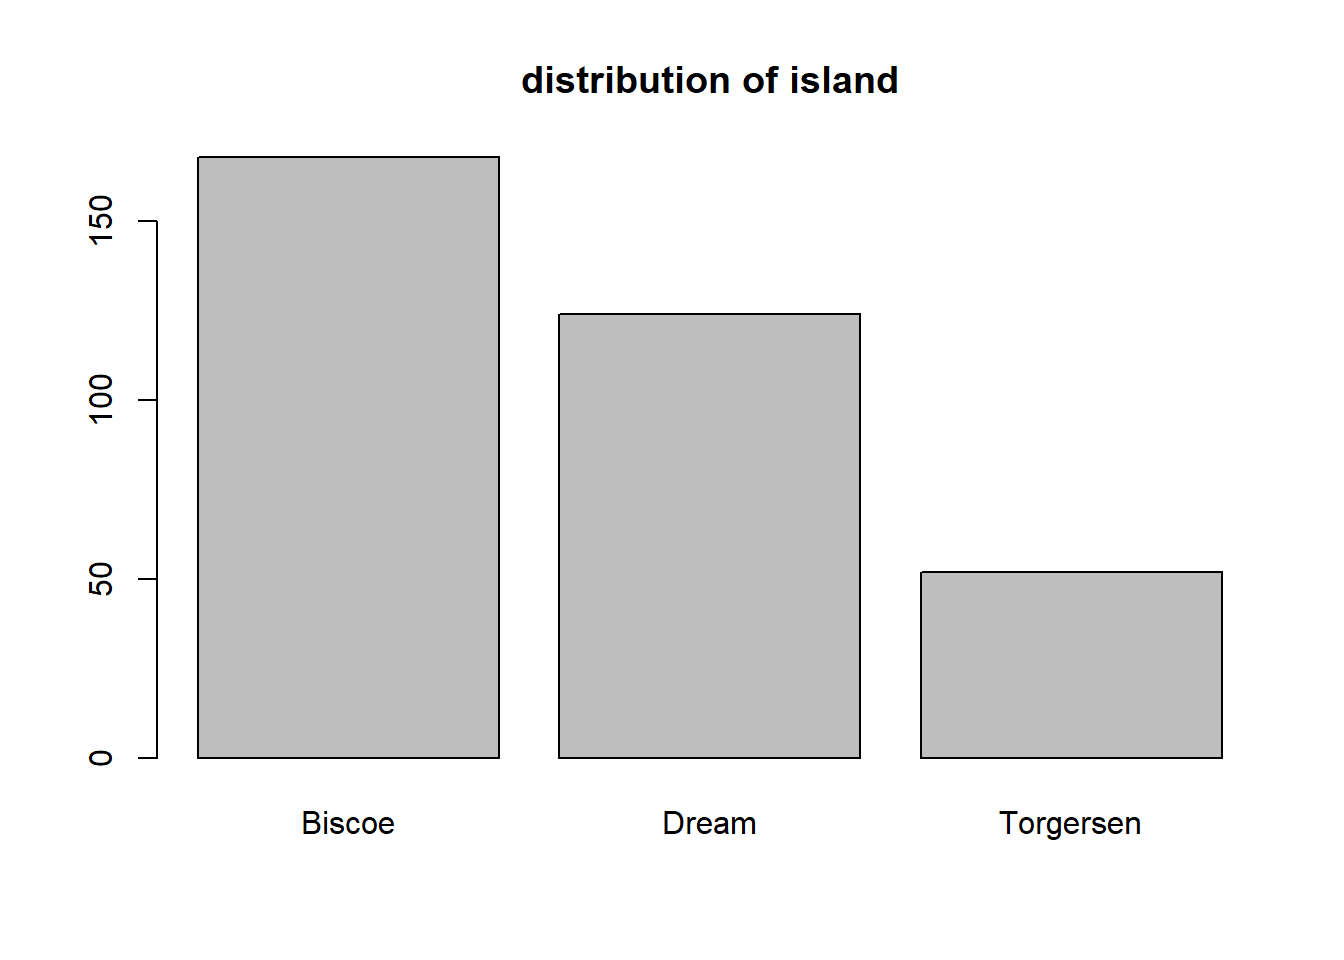
\includegraphics{A-Progessive-Introduction-to-Linear-Models_files/figure-latex/unnamed-chunk-64-1.pdf}

We see that the largest number of penguins were obserevd on Biscoe allowed, followed by Dream and Torgersen islands, respectively.

Alternatively, we can combine \texttt{barplot} with the \texttt{table} function. We do so below for the \texttt{sex} variable. To account for \texttt{NA}s in the \texttt{sex} variable, we specify \texttt{useNA\ =\ "ifany"} in the \texttt{table} function. Also, we specify \texttt{names.arg\ =\ ...} to specify the bar names, otherwise the bar for \texttt{NA} will be blank.

\begin{Shaded}
\begin{Highlighting}[]
\FunctionTok{barplot}\NormalTok{(}\FunctionTok{table}\NormalTok{(penguins\_clean}\SpecialCharTok{$}\NormalTok{sex, }\AttributeTok{useNA =} \StringTok{"ifany"}\NormalTok{),}
        \AttributeTok{names.arg =} \FunctionTok{c}\NormalTok{(}\StringTok{"female"}\NormalTok{, }\StringTok{"male"}\NormalTok{, }\StringTok{"NA"}\NormalTok{))}
\end{Highlighting}
\end{Shaded}

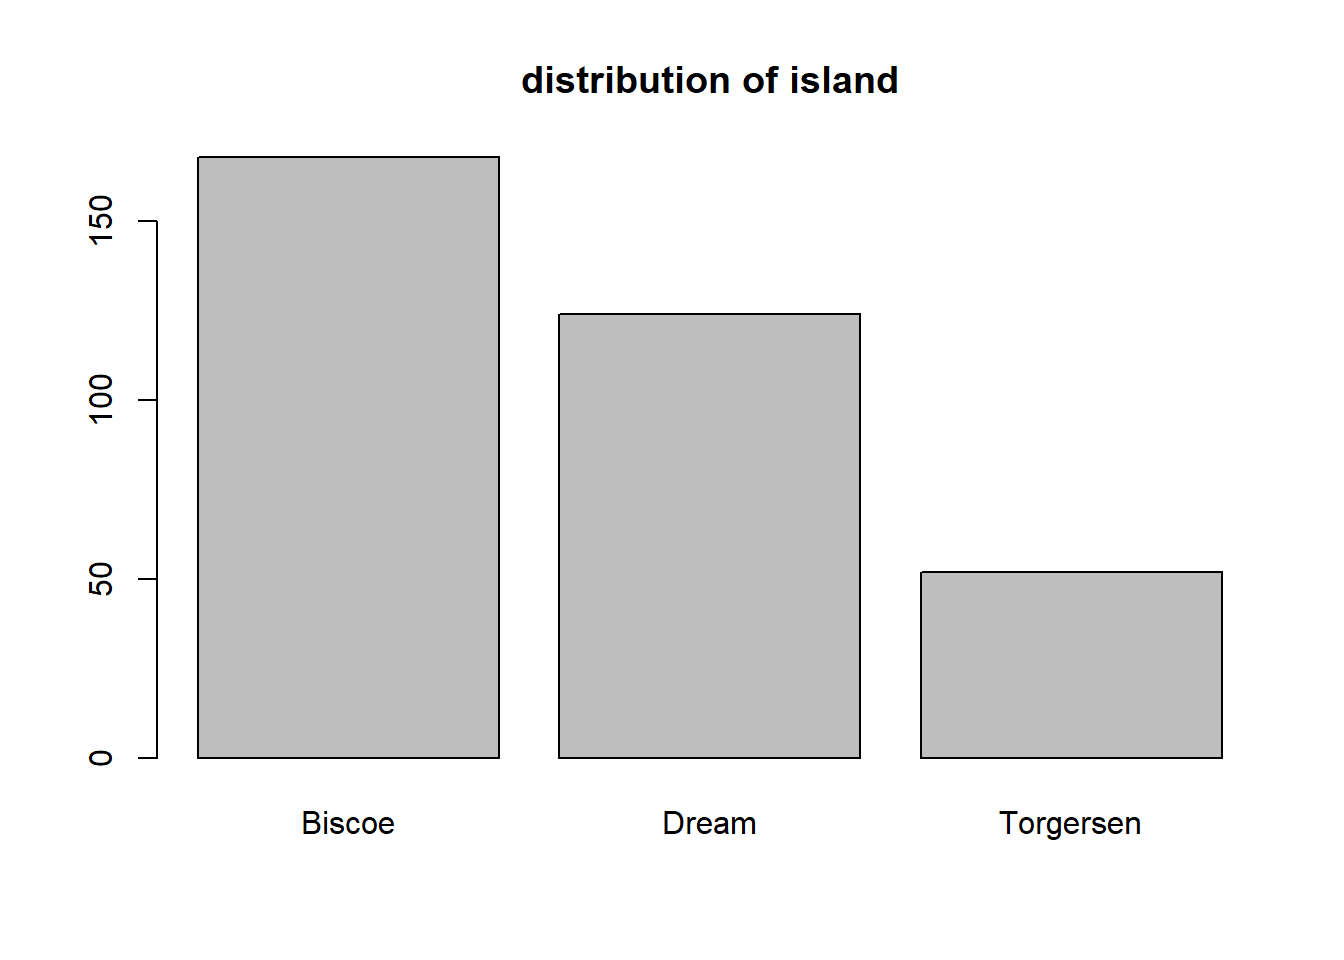
\includegraphics{A-Progessive-Introduction-to-Linear-Models_files/figure-latex/unnamed-chunk-65-1.pdf}

We see that that there are slightly more male than female penguins, with a handful of observations missing this characteristic.

To create a relatively frequency bar plot, we should divide the results of \texttt{table} by the number of relevant observations. For this particular example, we could use the code below. We use the \texttt{length} function to determine the number of observations to divide the counts with.

\begin{Shaded}
\begin{Highlighting}[]
\FunctionTok{barplot}\NormalTok{(}\FunctionTok{table}\NormalTok{(penguins\_clean}\SpecialCharTok{$}\NormalTok{sex, }\AttributeTok{useNA =} \StringTok{"ifany"}\NormalTok{) }\SpecialCharTok{/}
          \FunctionTok{length}\NormalTok{(penguins\_clean}\SpecialCharTok{$}\NormalTok{sex),}
        \AttributeTok{names.arg =} \FunctionTok{c}\NormalTok{(}\StringTok{"female"}\NormalTok{, }\StringTok{"male"}\NormalTok{, }\StringTok{"NA"}\NormalTok{))}
\end{Highlighting}
\end{Shaded}

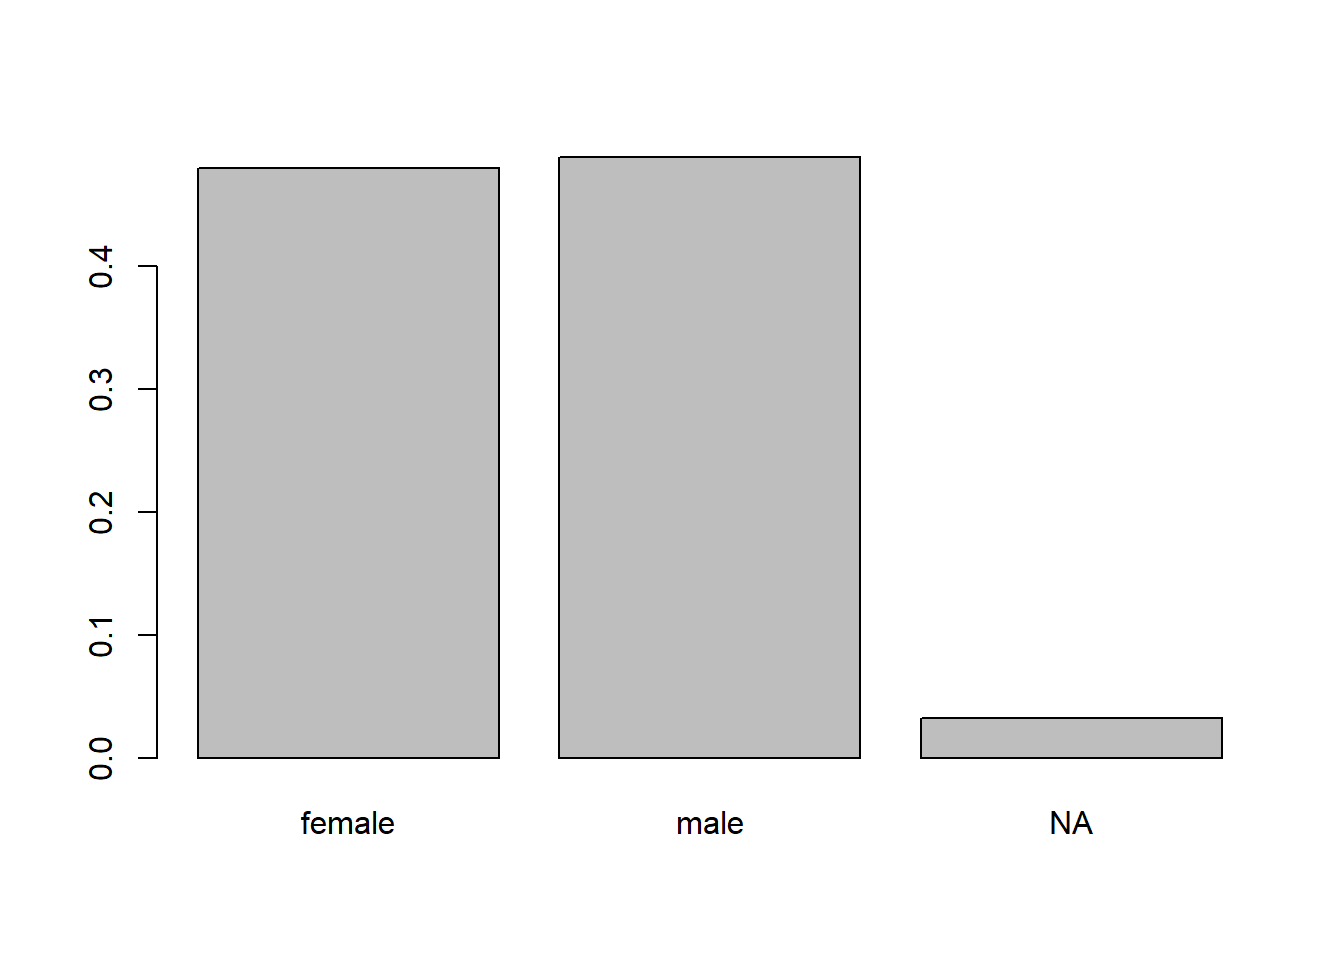
\includegraphics{A-Progessive-Introduction-to-Linear-Models_files/figure-latex/unnamed-chunk-66-1.pdf}

To create a bar plot with \textbf{ggplot2}, we first create a basic \texttt{ggplot} object containing our data. Make sure to load the \textbf{ggplot2} package prior to creating the plot, otherwise you'll get errors!

\begin{Shaded}
\begin{Highlighting}[]
\CommentTok{\# load ggplot2 package}
\FunctionTok{library}\NormalTok{(ggplot2)}
\CommentTok{\# create generic ggplot object with our data}
\NormalTok{gg\_penguin }\OtherTok{\textless{}{-}} \FunctionTok{ggplot}\NormalTok{(}\AttributeTok{data =}\NormalTok{ penguins\_clean)}
\end{Highlighting}
\end{Shaded}

\texttt{gg\_penguin} is a minimal \texttt{ggplot} object with the raw information needed to produce future graphics. To create a bar plot, we add the geom \texttt{geom\_bar} and map the \texttt{species} variable (in this example) to the \texttt{x} aesthetic using the \texttt{aes} function.

\begin{Shaded}
\begin{Highlighting}[]
\CommentTok{\# create bar plot for species variable}
\NormalTok{gg\_penguin }\SpecialCharTok{+} \FunctionTok{geom\_bar}\NormalTok{(}\FunctionTok{aes}\NormalTok{(}\AttributeTok{x =}\NormalTok{ species))}
\end{Highlighting}
\end{Shaded}

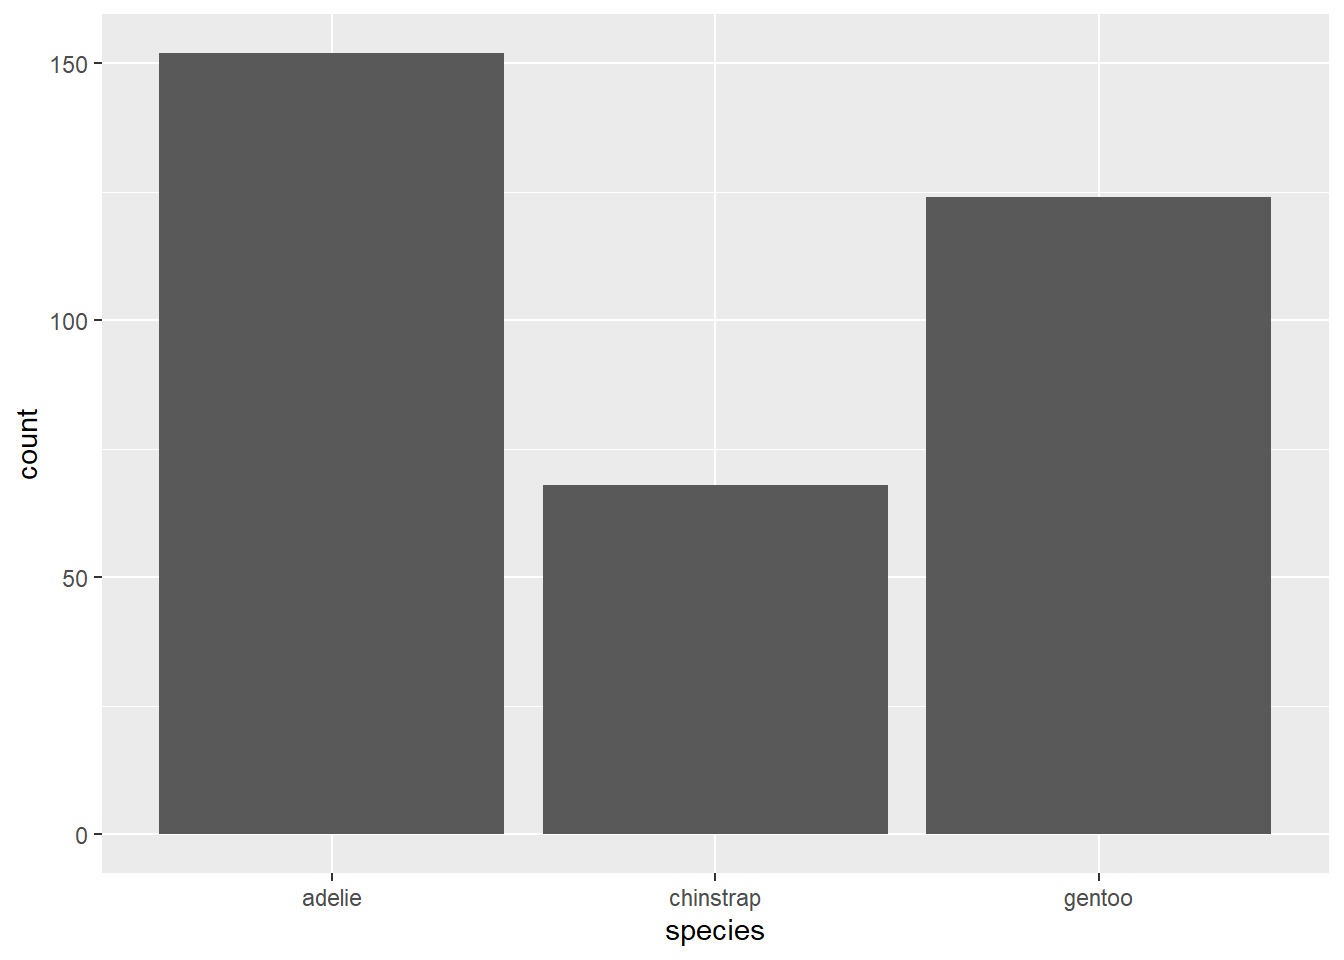
\includegraphics{A-Progessive-Introduction-to-Linear-Models_files/figure-latex/unnamed-chunk-68-1.pdf}

\hypertarget{box-plots}{%
\subsubsection{Box plots}\label{box-plots}}

A box plot is a simple graphic showing critical quantiles of a \texttt{numeric} variable, as well as outliers. A box plot indicates the median, 0.25 quantile (Q1), 0.75 quantile (Q3), and extend bars to the largest and smallest observations that are not outliers. Outliers are usually marked with starts or dots. The standard definition of an outlier in the context of box plots is an value that is more than Q3 + 1.5 (Q3 - Q1) and less than Q1 - 1.5 (Q3 - Q1). The box of a box plot extends from Q1 to Q3, with a line in the box indicating the median.

Box plots are useful for identifying outliers and skewness in the variable. However, box plot throw away a lot of information, so be cautious in making conclusions about skewness and modality without seeking a histogram or density plot of the data.

The \texttt{boxplot} function is the easiest approach for producing a box plot using base R. We do so for the \texttt{body\_mass} variable below.

\begin{Shaded}
\begin{Highlighting}[]
\FunctionTok{boxplot}\NormalTok{(penguins\_clean}\SpecialCharTok{$}\NormalTok{body\_mass,}
        \AttributeTok{main =} \StringTok{"distribution of body mass"}\NormalTok{)}
\end{Highlighting}
\end{Shaded}

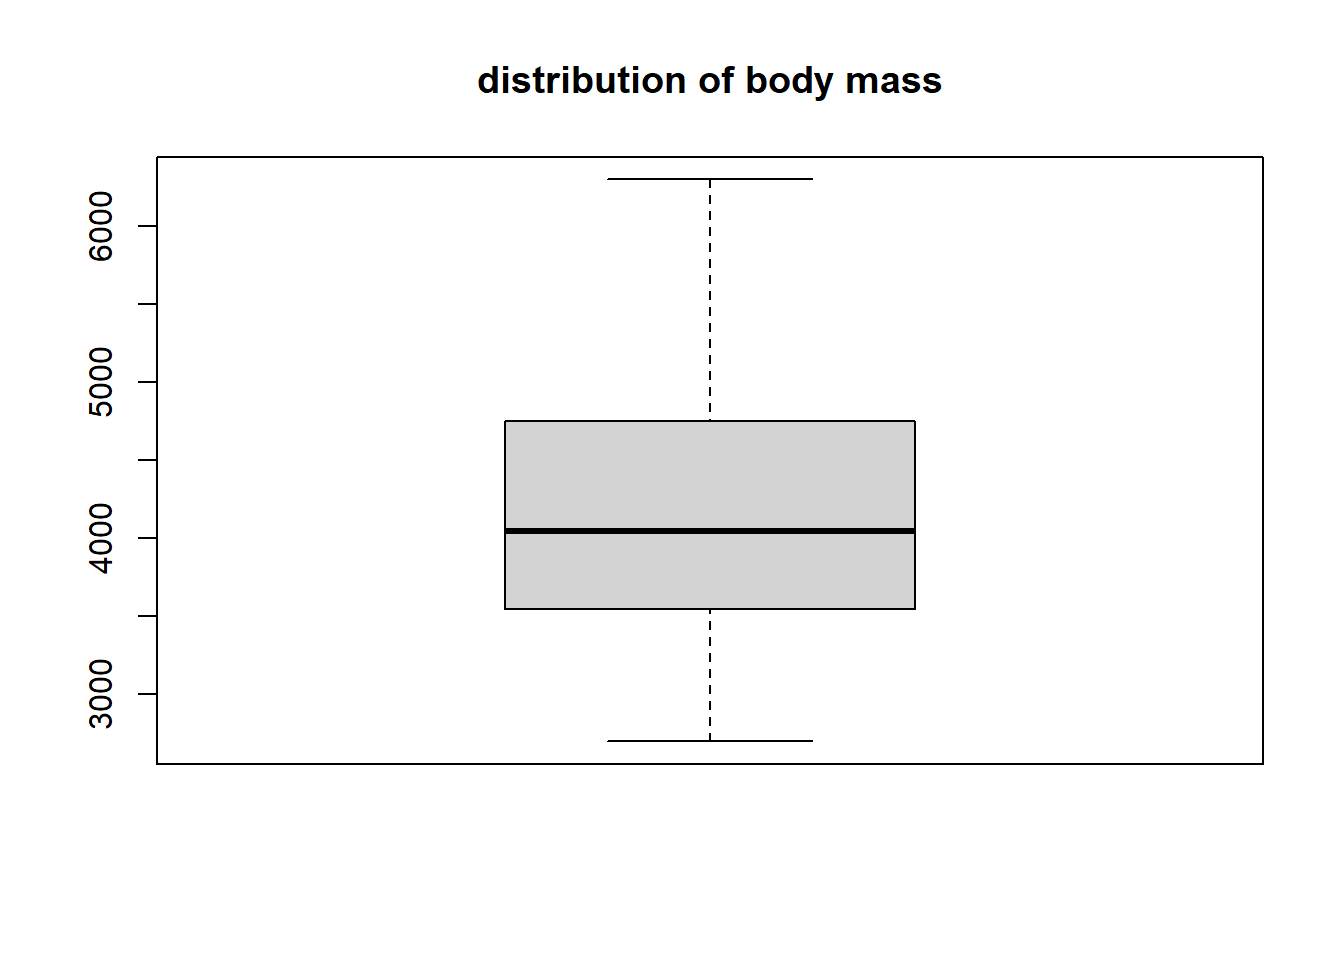
\includegraphics{A-Progessive-Introduction-to-Linear-Models_files/figure-latex/unnamed-chunk-69-1.pdf}

The \texttt{body\_mass} variable doesn't have any outliers. It's has perhaps a slight positive skew since the upper tail and upper part of the box are longer than the lower tail and lower part of the box. The median value is a bit larger than 4000 grams, while 50\% of the data being between approximatly 3500 and 4750 grams (i.e., between Q1 and Q3).

To create a box plot using \textbf{ggplot2}, we use \texttt{geom\_boxplot}. We create a box plot for the \texttt{bill\_length} variable below. We map \texttt{bill\_length} to the \texttt{y} aesthetic so that we get a vertically-oriented box plot (mapping it to \texttt{x} will produce a horizontal box plot).

\begin{Shaded}
\begin{Highlighting}[]
\NormalTok{gg\_penguin }\SpecialCharTok{+} \FunctionTok{geom\_boxplot}\NormalTok{(}\FunctionTok{aes}\NormalTok{(}\AttributeTok{y =}\NormalTok{ bill\_length))}
\DocumentationTok{\#\# Warning: Removed 2 rows containing non{-}finite values}
\DocumentationTok{\#\# (\textasciigrave{}stat\_boxplot()\textasciigrave{}).}
\end{Highlighting}
\end{Shaded}

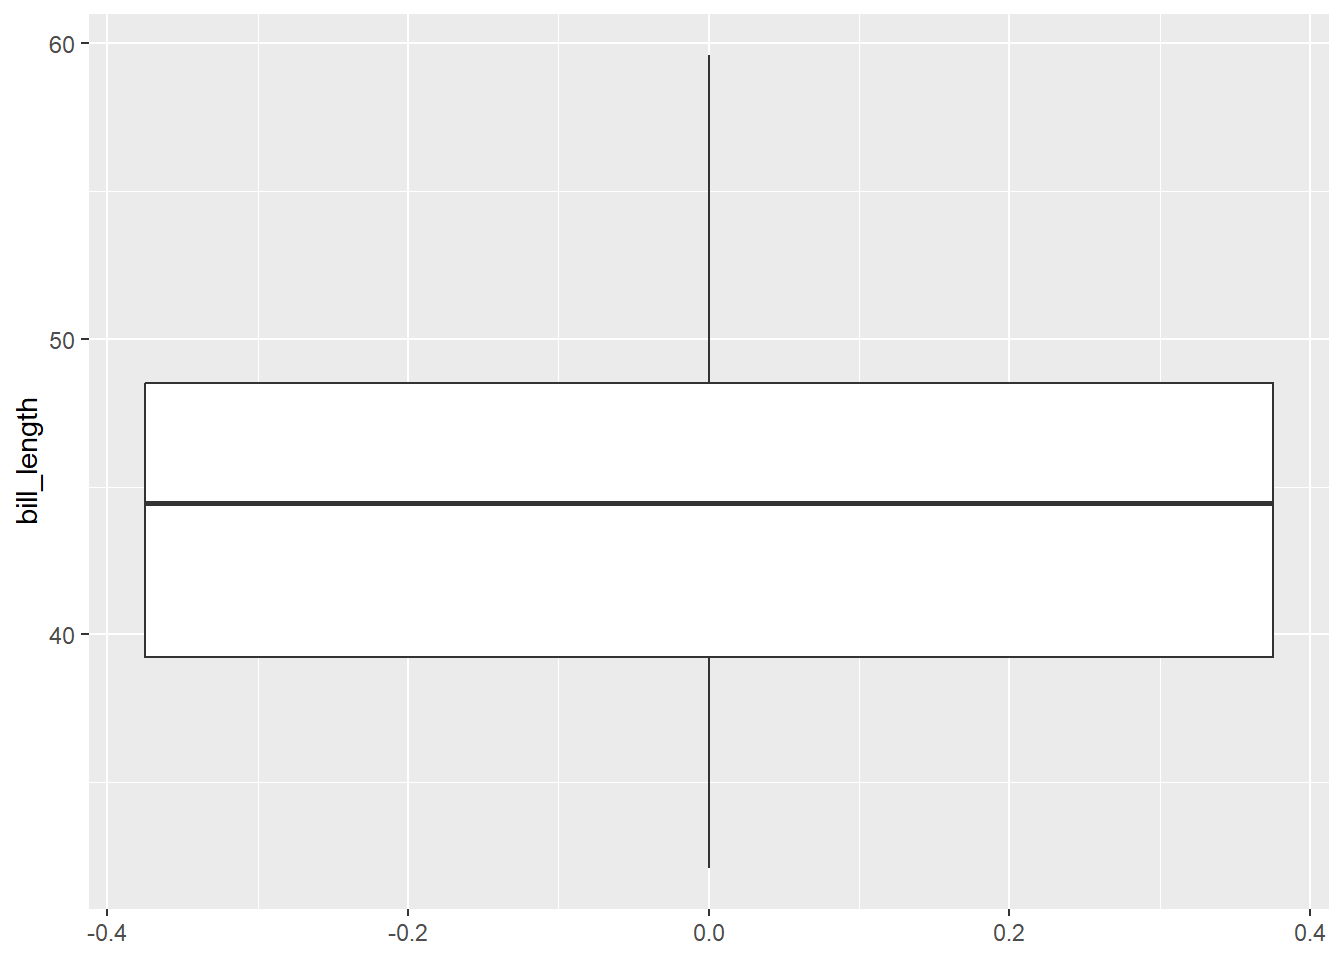
\includegraphics{A-Progessive-Introduction-to-Linear-Models_files/figure-latex/unnamed-chunk-70-1.pdf}

There are not \texttt{bill\_length} outliers. The minimum value is approximately 32 mm and the maximum is almost 60 mm. Q1 is approximately 39 mm, the median is approximately 44 mm, and Q3 is approximately 48 mm. It is difficult to assess the skewness of this data. The upper tail is longer than the shorter tail, but the upper box is shorter than the lower box, so the evidence is inconsistent.

\hypertarget{histograms}{%
\subsubsection{Histograms}\label{histograms}}

A histogram displays the distribution of a \texttt{numeric} variable. A histogram counts the number of values falling into (usually) equal-sized ``bins'' running from the smallest value to the largest value. The number of bins and width of the bins affect the shape of the histogram.

Histograms are used to assess skewness, modality (the number of clear ``peaks'' in the plot), and to some extent, outliers.

The \texttt{hist} function is used create a histogram of a \texttt{numeric} variable. We augment the information already learned about \texttt{bill\_length} with a histogram in the code below.

\begin{Shaded}
\begin{Highlighting}[]
\FunctionTok{hist}\NormalTok{(penguins\_clean}\SpecialCharTok{$}\NormalTok{bill\_length)}
\end{Highlighting}
\end{Shaded}

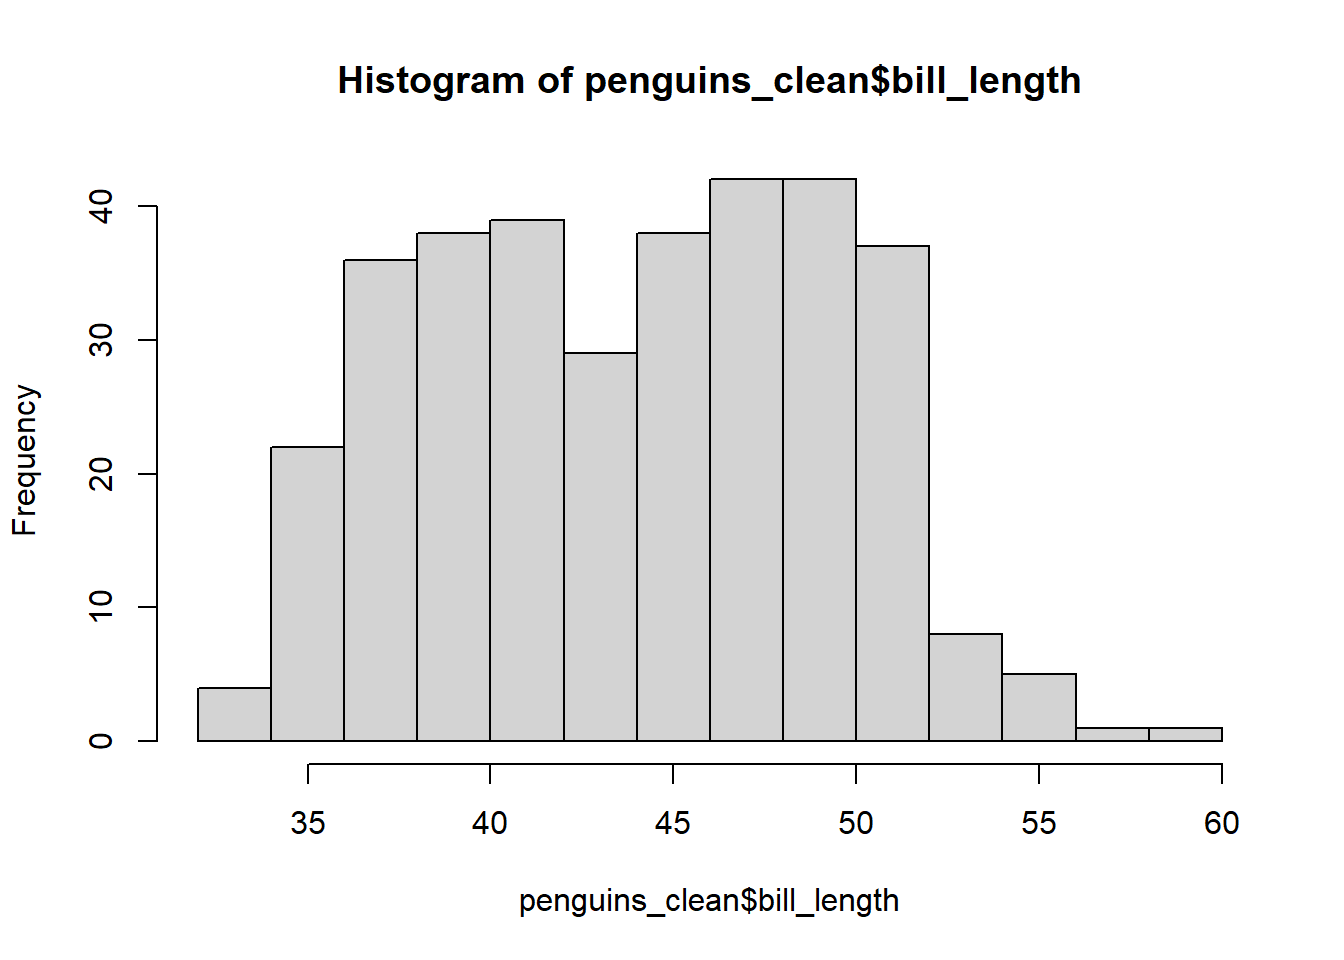
\includegraphics{A-Progessive-Introduction-to-Linear-Models_files/figure-latex/unnamed-chunk-71-1.pdf}

The title and x-axis label are visually unappealling, so we use the \texttt{main} and \texttt{xlab} arguments to change them to nothing (i.e., no title) and \texttt{bill\ length\ (mm)}. We also increase the number of bins using the \texttt{breaks} argument.

\begin{Shaded}
\begin{Highlighting}[]
\FunctionTok{hist}\NormalTok{(penguins\_clean}\SpecialCharTok{$}\NormalTok{bill\_length, }\AttributeTok{main =} \StringTok{""}\NormalTok{,}
     \AttributeTok{xlab =} \StringTok{"bill length (mm)"}\NormalTok{, }\AttributeTok{breaks =} \DecValTok{20}\NormalTok{)}
\end{Highlighting}
\end{Shaded}

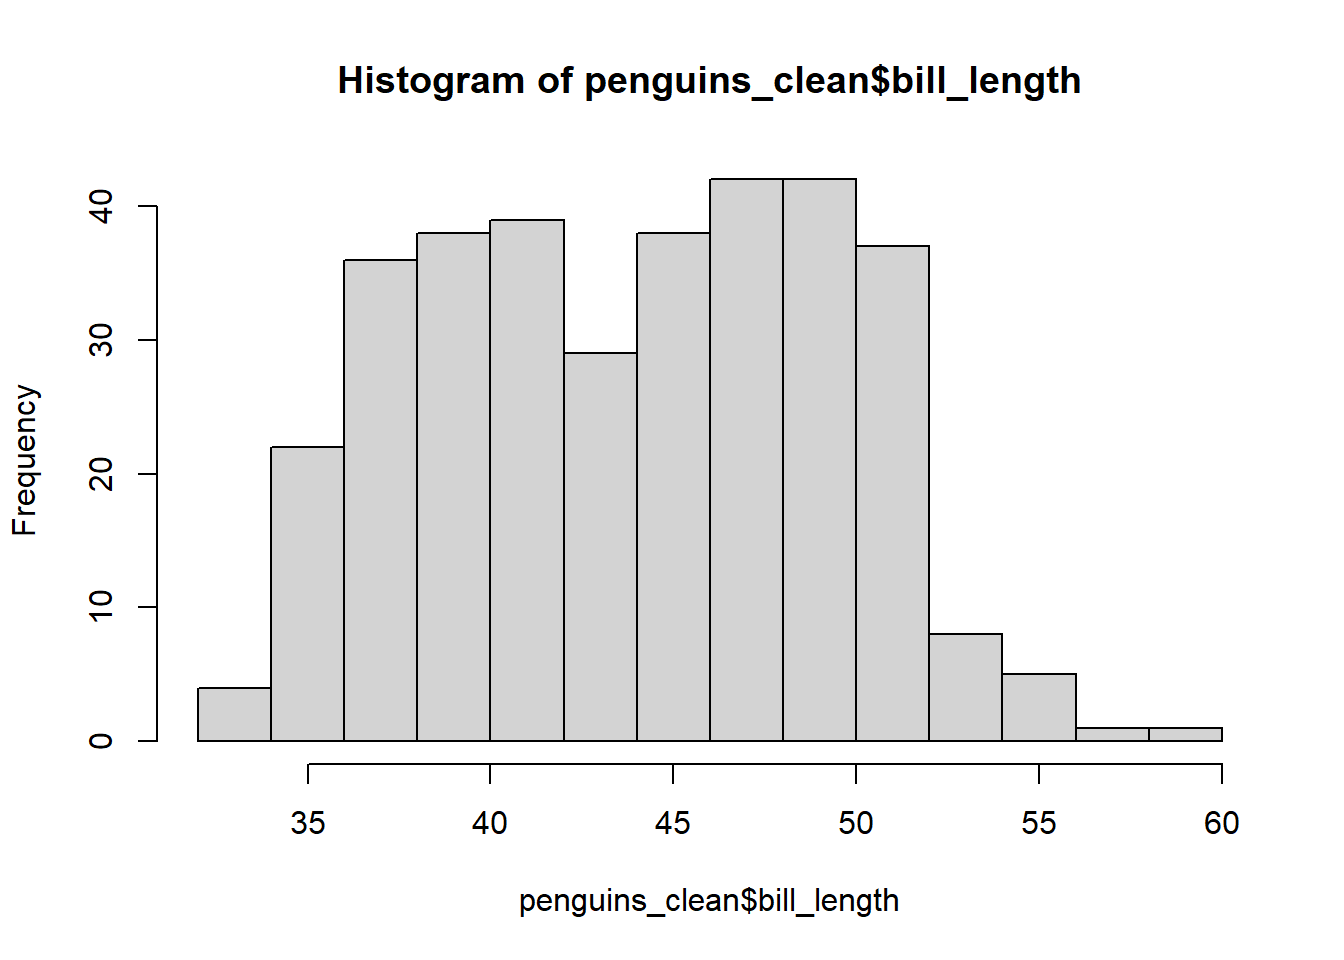
\includegraphics{A-Progessive-Introduction-to-Linear-Models_files/figure-latex/unnamed-chunk-72-1.pdf}

This distribution of \texttt{bill\_length} is bimodal (has two prominent peaks or modes). That is why the skewness information on the box plot of \texttt{bill\_length} was inconsistent. This also demonstrates why should should never draw conclusions like modality or skewness from numeric summaries alone.

We use \texttt{geom\_histogram} to create a histogram using \textbf{ggplot2}, mapping the variable to the \texttt{x} aesthetic. We do so for the \texttt{flipper\_length} variable below.

\begin{Shaded}
\begin{Highlighting}[]
\NormalTok{gg\_penguin }\SpecialCharTok{+} \FunctionTok{geom\_histogram}\NormalTok{(}\FunctionTok{aes}\NormalTok{(}\AttributeTok{x =}\NormalTok{ flipper\_length))}
\DocumentationTok{\#\# \textasciigrave{}stat\_bin()\textasciigrave{} using \textasciigrave{}bins = 30\textasciigrave{}. Pick better value with}
\DocumentationTok{\#\# \textasciigrave{}binwidth\textasciigrave{}.}
\DocumentationTok{\#\# Warning: Removed 2 rows containing non{-}finite values}
\DocumentationTok{\#\# (\textasciigrave{}stat\_bin()\textasciigrave{}).}
\end{Highlighting}
\end{Shaded}

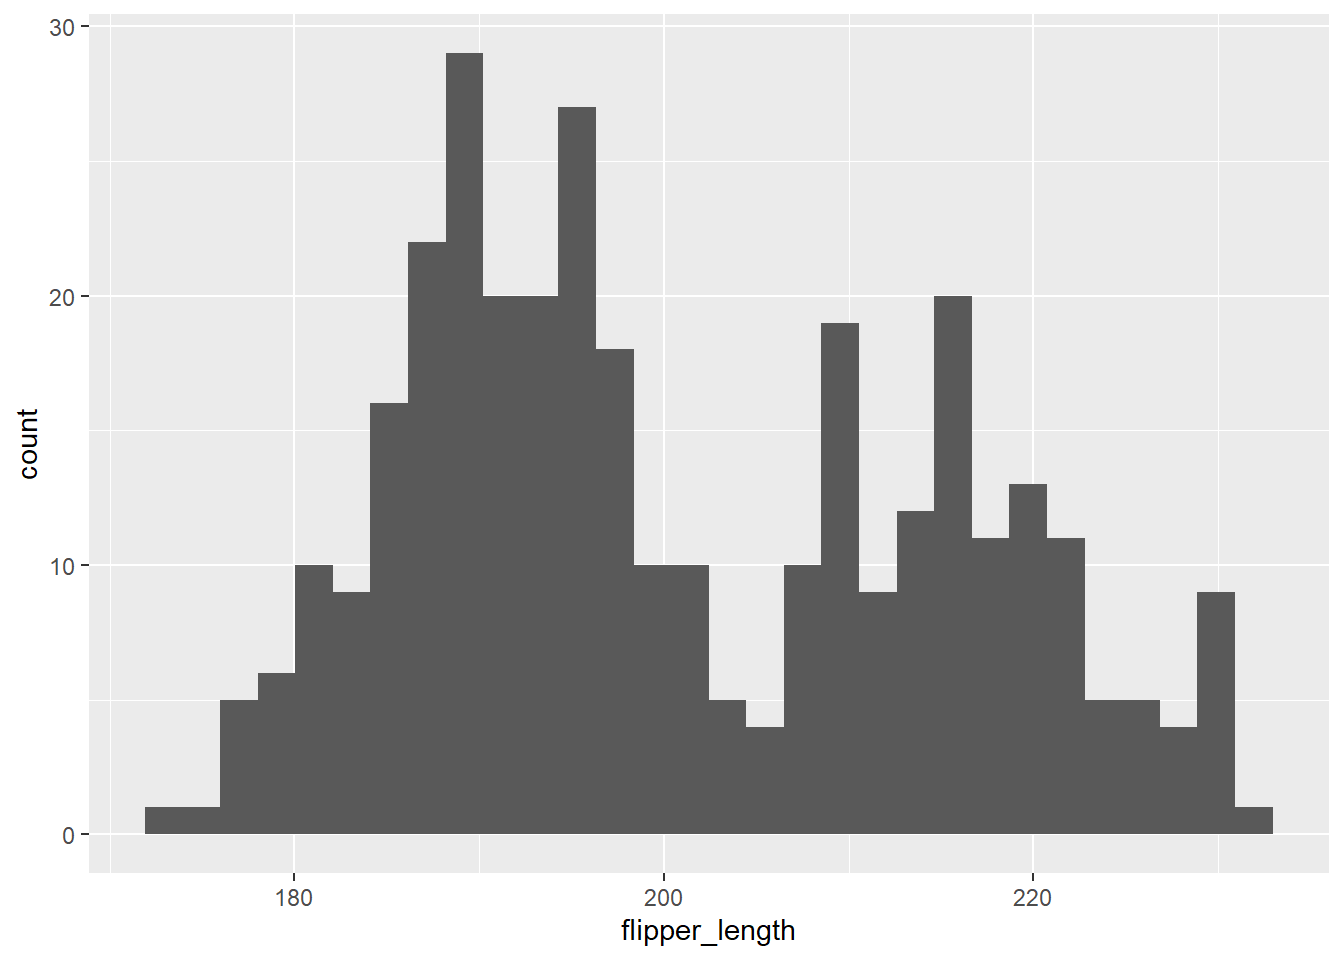
\includegraphics{A-Progessive-Introduction-to-Linear-Models_files/figure-latex/unnamed-chunk-73-1.pdf}

Flipper length is also bimodal, with prominent peaks approximately centered around 190 and 220 mm.

\hypertarget{density-plots}{%
\subsubsection{Density plots}\label{density-plots}}

A density plot is similar to a smoothed histogram and the area under the smoothed curve must equal 1. In general, density plots are more visually appealing than histograms, but both communicate similar information. However, density plots can sometimes have problems near the edges of a variable with a fixed upper or lower bound because it is difficult to know how to smooth the data in that case.

The \texttt{plot} and \texttt{density} function can be combined to construct a density plot using \textbf{base} R. We do that below for the \texttt{bill\_depth} variable below. Note the use of \texttt{na.rm} to remove \texttt{NA} that would otherwise poison the density calculation, and use \texttt{main} to have a blank title.

\begin{Shaded}
\begin{Highlighting}[]
\FunctionTok{plot}\NormalTok{(}\FunctionTok{density}\NormalTok{(penguins\_clean}\SpecialCharTok{$}\NormalTok{bill\_depth, }\AttributeTok{na.rm =} \ConstantTok{TRUE}\NormalTok{), }\AttributeTok{main =} \StringTok{""}\NormalTok{)}
\end{Highlighting}
\end{Shaded}

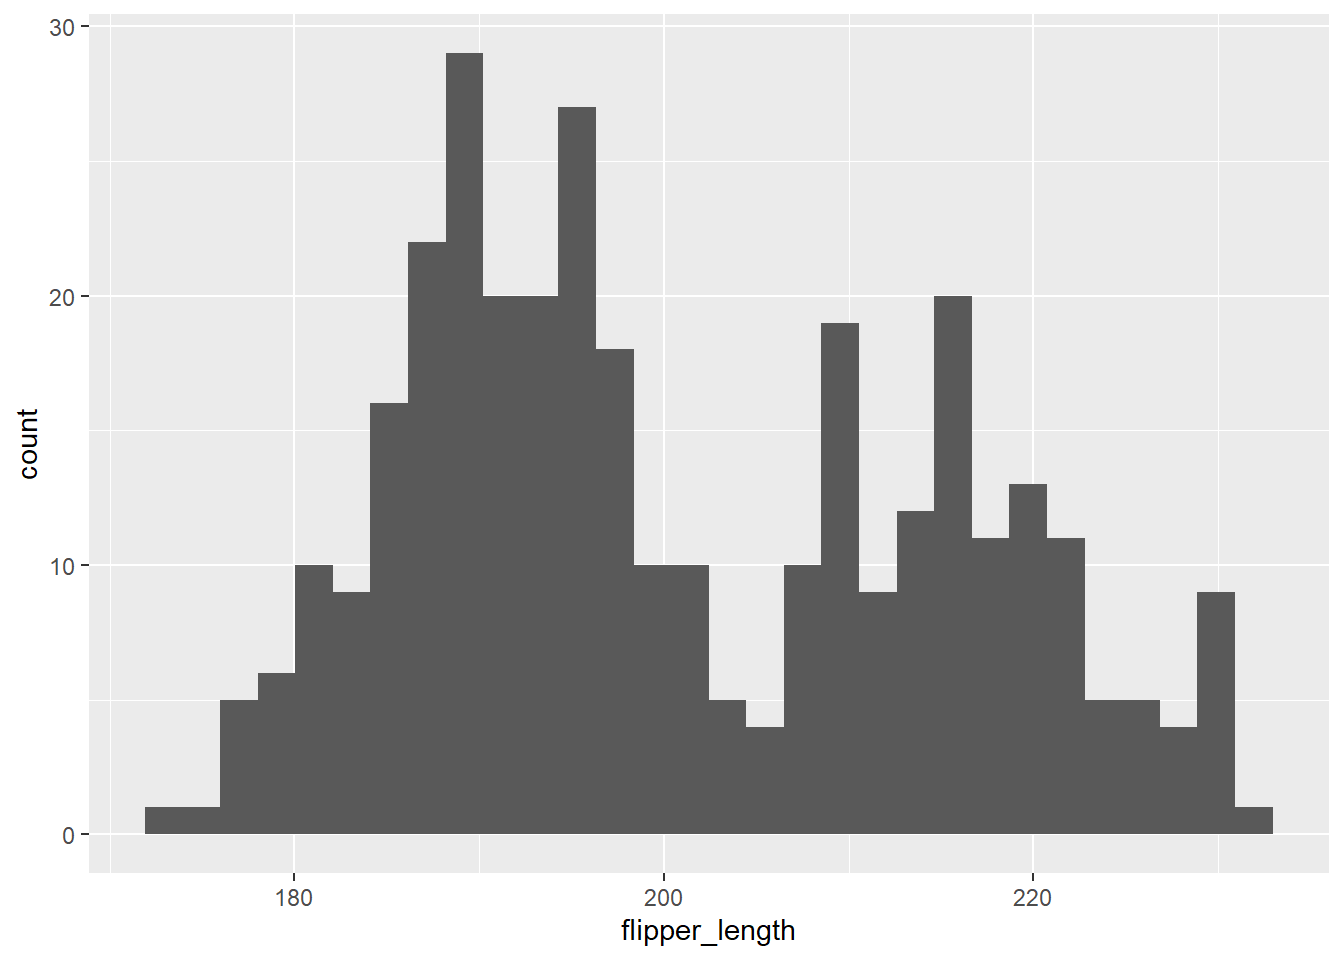
\includegraphics{A-Progessive-Introduction-to-Linear-Models_files/figure-latex/unnamed-chunk-74-1.pdf}
The \texttt{bill\_depth} variable is bimodal with peaks around 14 mm and 18 mm. The graphic also indicates that 342 observations were used to estimate the density and the bandwidth parameter was 0.5533. The bandwidth parameter controls the amount of smoothing and can be changed. Run \texttt{?stats::density} in the Console for more details.

We create a density plot with \textbf{ggplot2} using \texttt{geom\_density}. We do so for the \texttt{body\_mass} variable, mapping it to the \texttt{x} aesthetic.

\begin{Shaded}
\begin{Highlighting}[]
\NormalTok{gg\_penguin }\SpecialCharTok{+} \FunctionTok{geom\_density}\NormalTok{(}\FunctionTok{aes}\NormalTok{(}\AttributeTok{x =}\NormalTok{ body\_mass))}
\DocumentationTok{\#\# Warning: Removed 2 rows containing non{-}finite values}
\DocumentationTok{\#\# (\textasciigrave{}stat\_density()\textasciigrave{}).}
\end{Highlighting}
\end{Shaded}

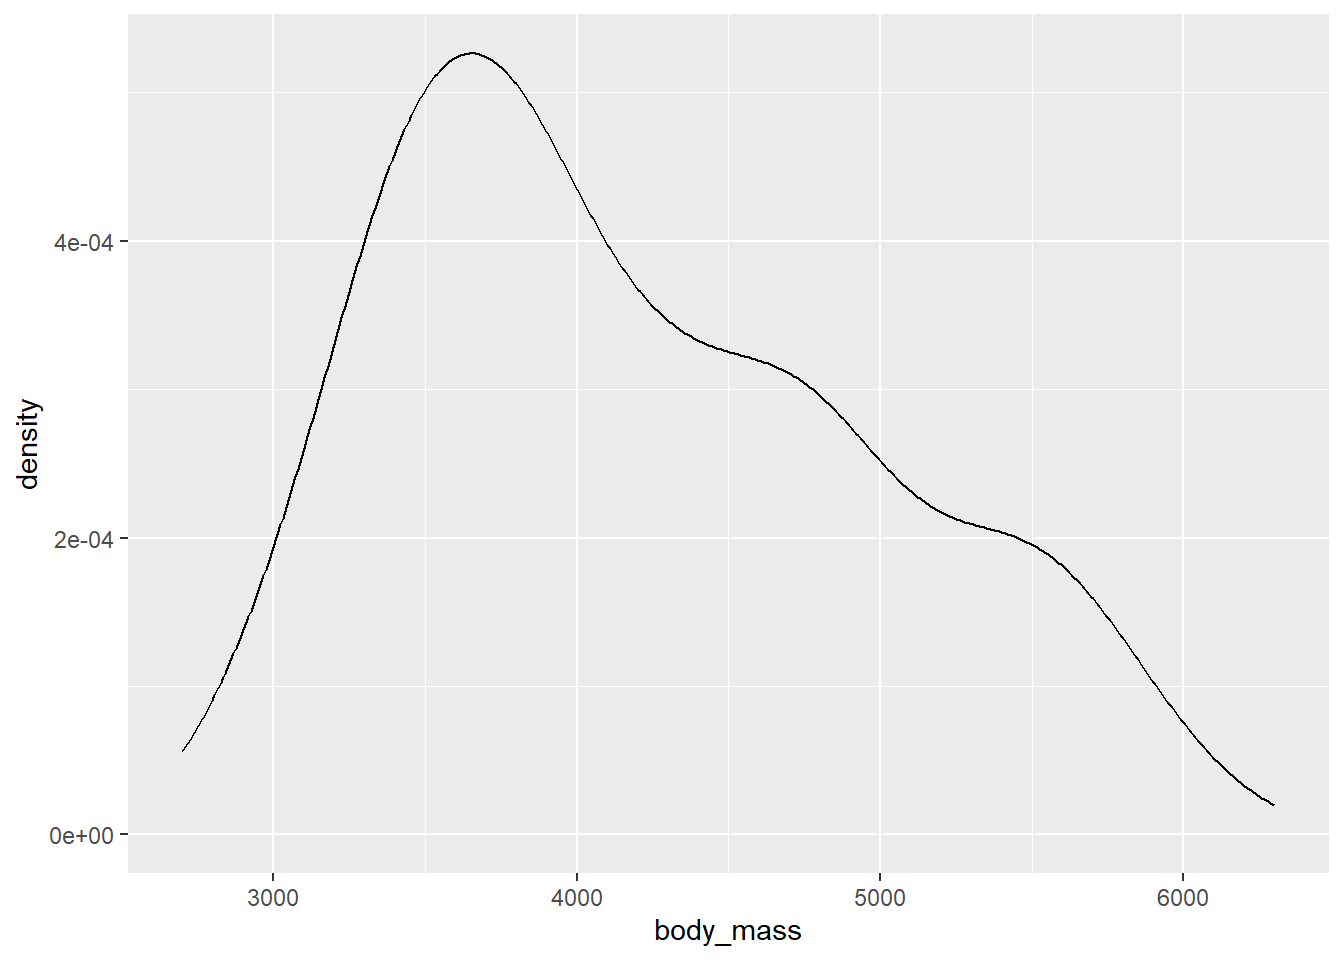
\includegraphics{A-Progessive-Introduction-to-Linear-Models_files/figure-latex/unnamed-chunk-75-1.pdf}

The \texttt{body\_mass} variable is unimodal, with a peak around 3700 grams. It is also positively skewed.

\hypertarget{bivariate-plots}{%
\subsection{Bivariate plots}\label{bivariate-plots}}

A \texttt{bivariate} plot is a plot involving two variables. A \texttt{bivariate} plot can involve more than one data type.

\hypertarget{scatter-plots}{%
\subsubsection{Scatter plots}\label{scatter-plots}}

Scatter plots can be used to identify the relationship between two \texttt{numeric} variables.

We use the \texttt{plot} function to create a scatter plot of \texttt{bill\_length} versus \texttt{body\_mass} (the \texttt{y} variable versus the \texttt{x} variable) using \textbf{base} R below. The \texttt{plot} function is very flexible and can be used multiple ways to produce a scatter plot, but we will use the \texttt{formula} method that takes a formula describing the variables (\texttt{y\ \textasciitilde{}\ x}) and the data frame from which the variables come.

\begin{Shaded}
\begin{Highlighting}[]
\CommentTok{\# xlab and ylab are used to customize the x{-}axis and y{-}axis labels}
\FunctionTok{plot}\NormalTok{(bill\_length }\SpecialCharTok{\textasciitilde{}}\NormalTok{ body\_mass, }\AttributeTok{data =}\NormalTok{ penguins\_clean,}
     \AttributeTok{xlab =} \StringTok{"body mass (g)"}\NormalTok{, }\AttributeTok{ylab =} \StringTok{"bill length (mm)"}\NormalTok{)}
\end{Highlighting}
\end{Shaded}

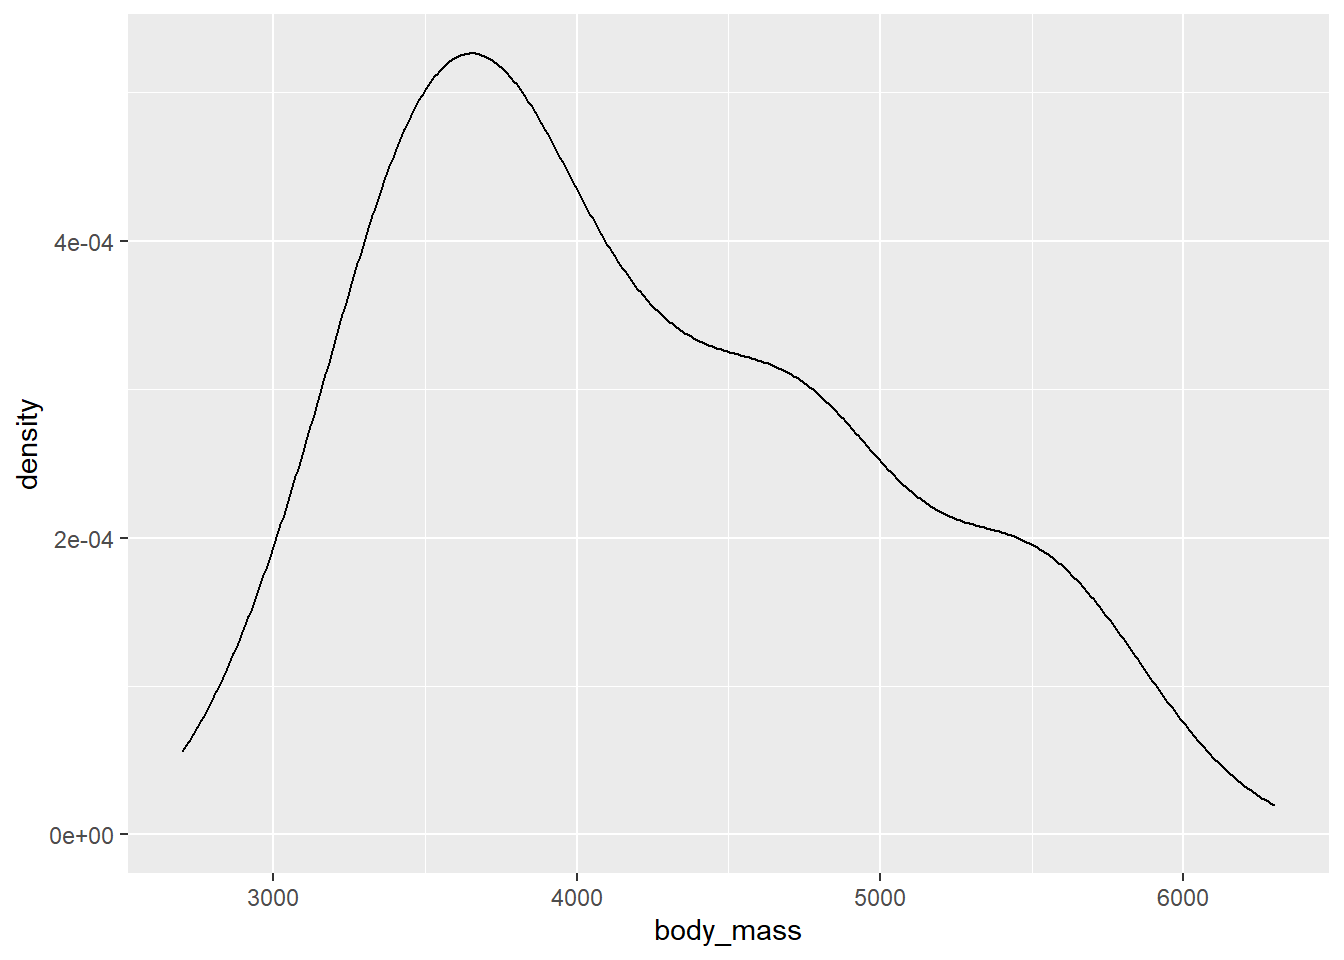
\includegraphics{A-Progessive-Introduction-to-Linear-Models_files/figure-latex/unnamed-chunk-76-1.pdf}

There is a positive linear relationship between \texttt{body\_mass} and \texttt{bill\_length}. As \texttt{body\_mass} increases, \texttt{bill\_length} tends to increase.

The \texttt{geom\_point} function can be used to create a scatter plot with \textbf{ggplot2}. we make the variables to be plotted to the \texttt{x} and \texttt{y} aesthetics. We create a scatter plot of \texttt{bill\_length} versus \texttt{bill\_depth}.

\begin{Shaded}
\begin{Highlighting}[]
\NormalTok{gg\_penguin }\SpecialCharTok{+} \FunctionTok{geom\_point}\NormalTok{(}\FunctionTok{aes}\NormalTok{(}\AttributeTok{x =}\NormalTok{ bill\_depth, }\AttributeTok{y =}\NormalTok{ bill\_length))}
\DocumentationTok{\#\# Warning: Removed 2 rows containing missing values}
\DocumentationTok{\#\# (\textasciigrave{}geom\_point()\textasciigrave{}).}
\end{Highlighting}
\end{Shaded}

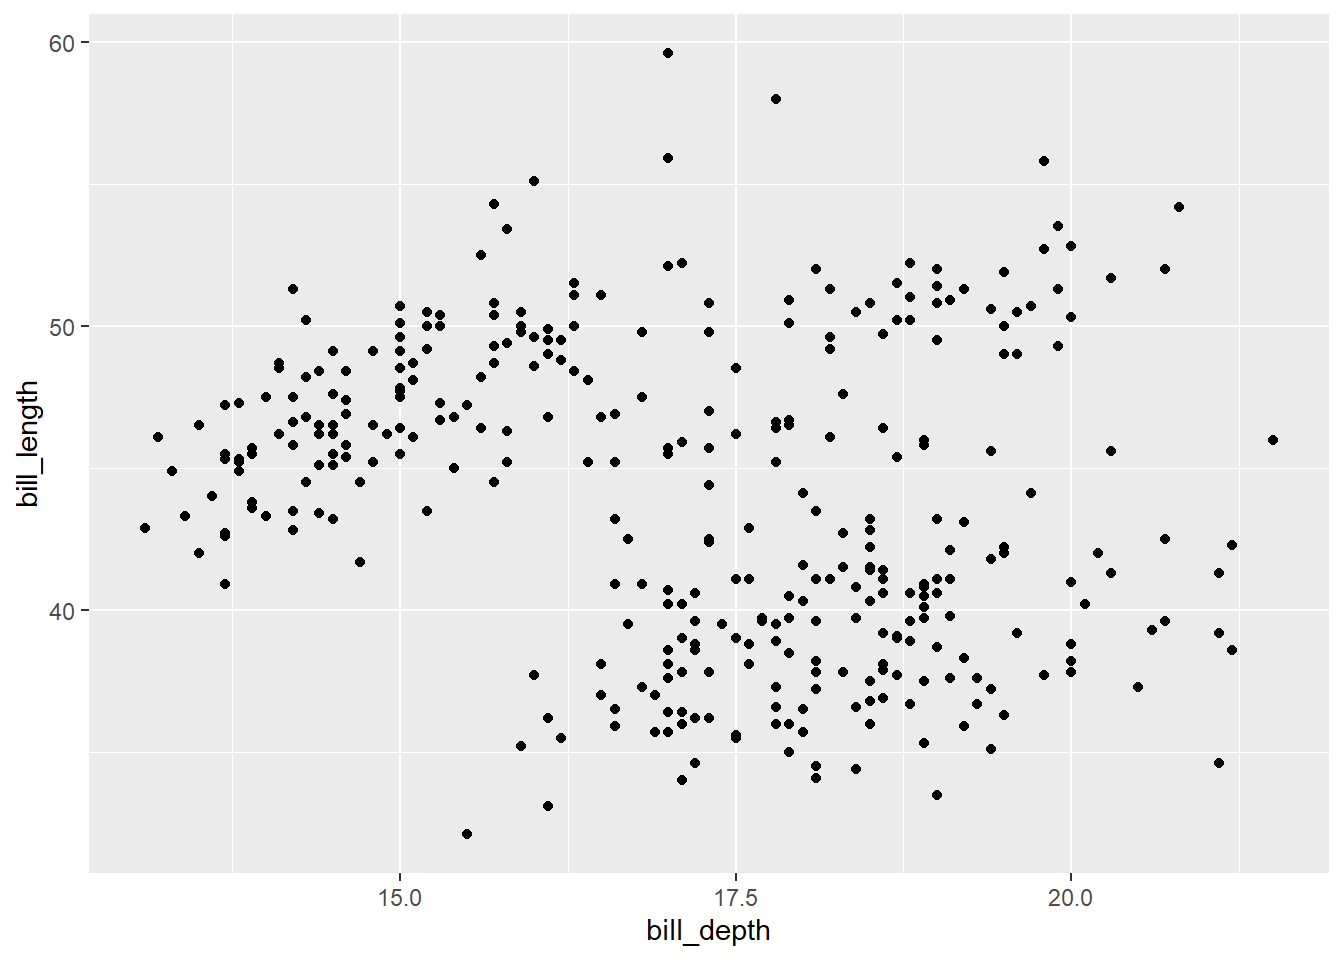
\includegraphics{A-Progessive-Introduction-to-Linear-Models_files/figure-latex/unnamed-chunk-77-1.pdf}

It's difficult to make any definitive conclusion about the relationship of these two variables from this plot, as the plot is basically a blob of points.

\hypertarget{parallel-box-plots}{%
\subsubsection{Parallel box plots}\label{parallel-box-plots}}

A parallel box plot is used to display the distribution of a \texttt{numeric} variable whose values are grouped based on each \texttt{level} of a \texttt{factor} variable. Specifically, a box plot of the \texttt{numeric} variable is is constructed for all the values associated with the levels of the \texttt{factor}. Parallel box plot are useful for determining if the distribution of a \texttt{numeric} variable substantially changes based on whether an observation has a certain \texttt{level} of a \texttt{factor}.

Once again use the \texttt{plot} function with a \texttt{formula}, we can create a parallel box plot easily, with the syntax of the formula being \texttt{numeric\ variable\ \textasciitilde{}\ factor\ variable} (you can reverse these to change the box plot orientation). We parallel box plots of \texttt{body\_mass} versus \texttt{sex} below.

\begin{Shaded}
\begin{Highlighting}[]
\FunctionTok{plot}\NormalTok{(body\_mass }\SpecialCharTok{\textasciitilde{}}\NormalTok{ sex, }\AttributeTok{data =}\NormalTok{ penguins\_clean)}
\end{Highlighting}
\end{Shaded}

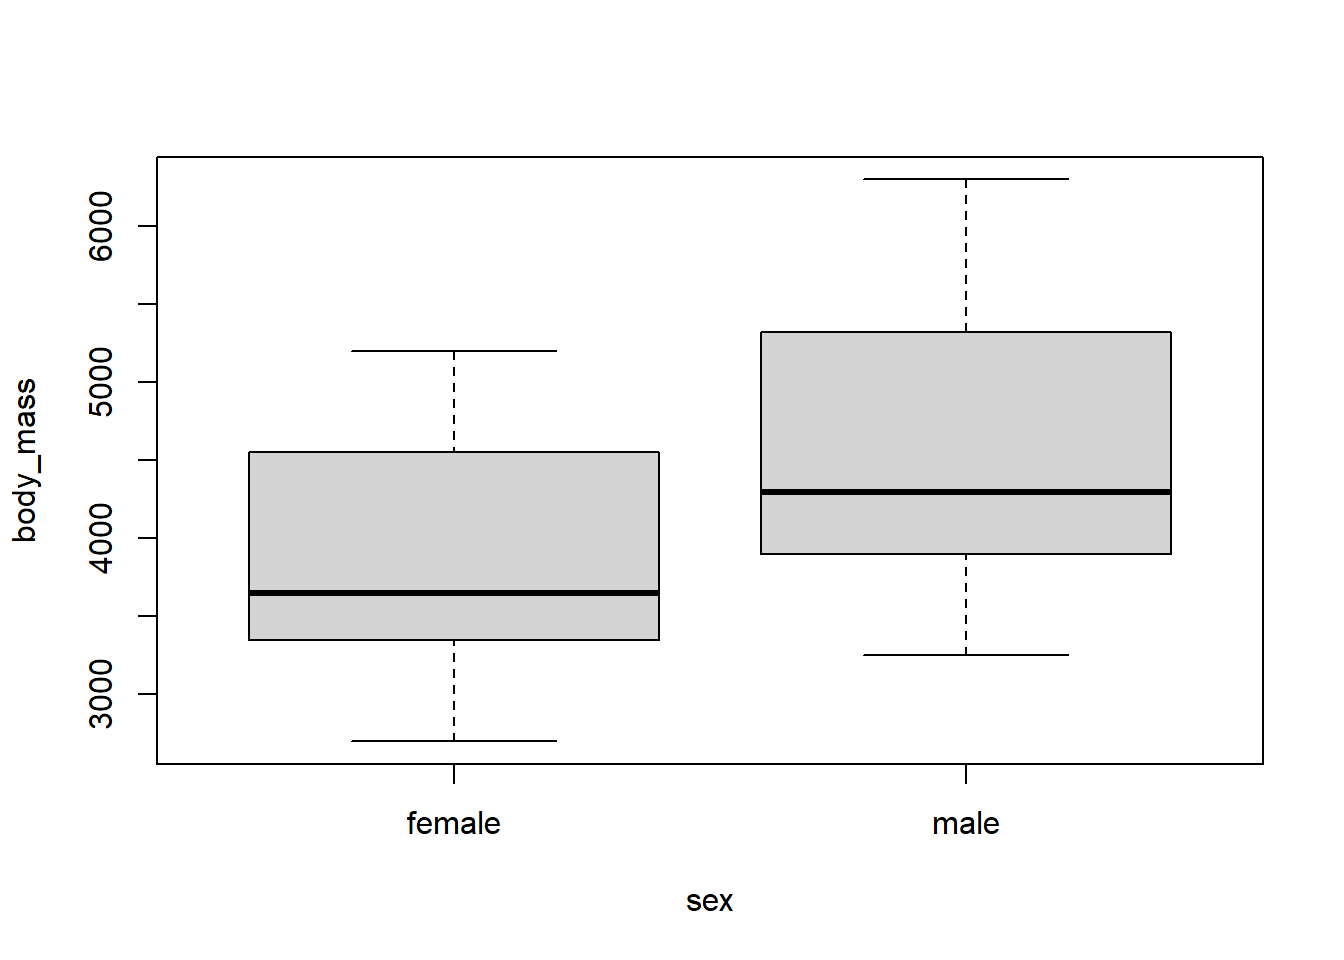
\includegraphics{A-Progessive-Introduction-to-Linear-Models_files/figure-latex/unnamed-chunk-78-1.pdf}

We can see that the \texttt{body\_mass} values tend to be larger for the male penguins compared to the female penguins.

We can produce something similar with \textbf{ggplot2} by specifying both the \texttt{y} and \texttt{x} aesthetics of for \texttt{geom\_boxplot}. We do so below to compare \texttt{bill\_length} for the different penguin \texttt{species}.

\begin{Shaded}
\begin{Highlighting}[]
\NormalTok{gg\_penguin }\SpecialCharTok{+} \FunctionTok{geom\_boxplot}\NormalTok{(}\FunctionTok{aes}\NormalTok{(}\AttributeTok{x =}\NormalTok{ species, }\AttributeTok{y =}\NormalTok{ bill\_length))}
\DocumentationTok{\#\# Warning: Removed 2 rows containing non{-}finite values}
\DocumentationTok{\#\# (\textasciigrave{}stat\_boxplot()\textasciigrave{}).}
\end{Highlighting}
\end{Shaded}

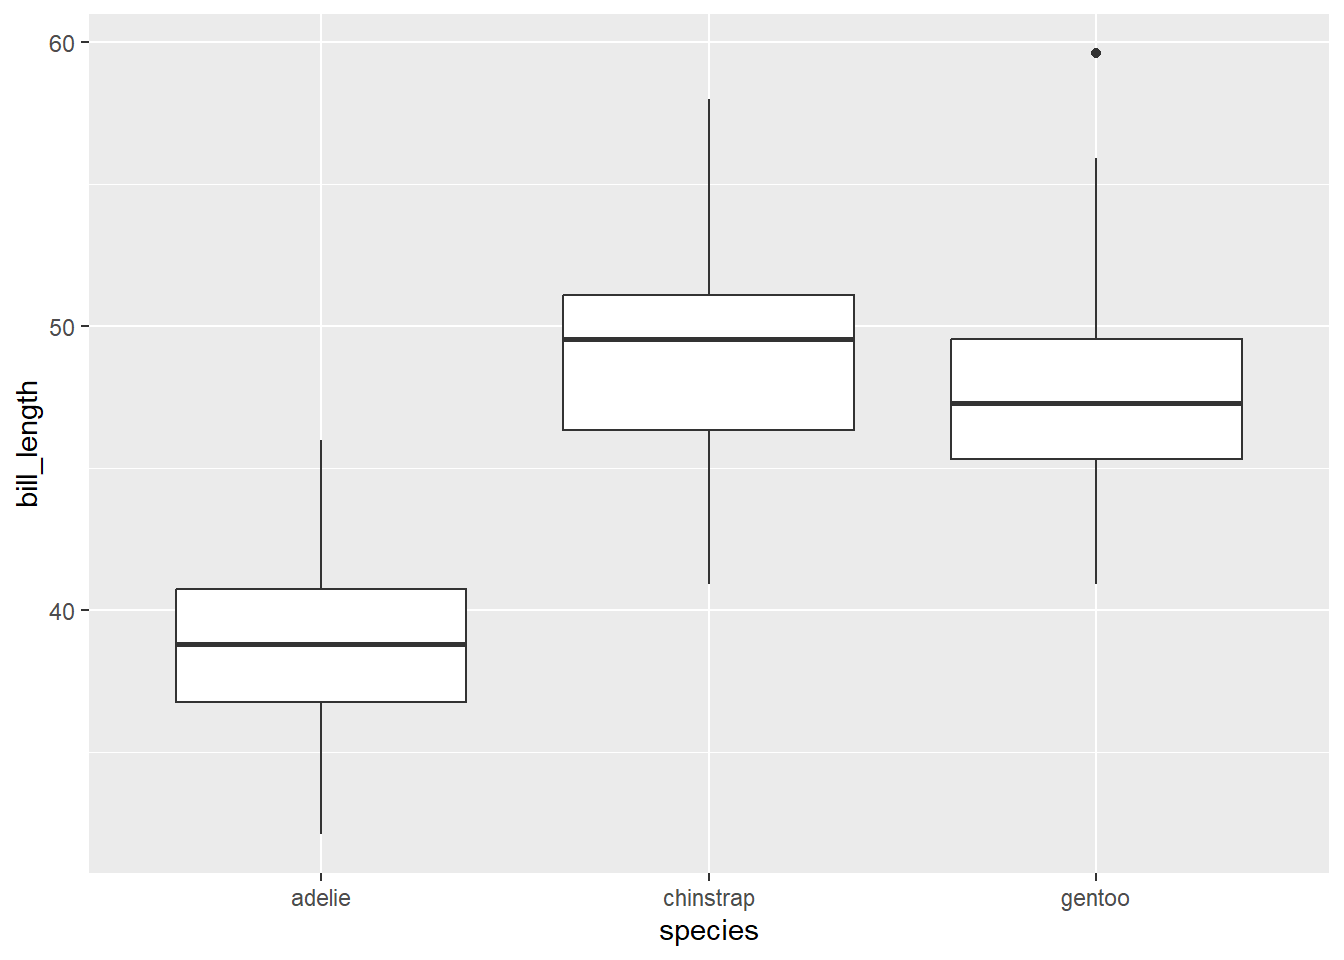
\includegraphics{A-Progessive-Introduction-to-Linear-Models_files/figure-latex/unnamed-chunk-79-1.pdf}

From a quick glance, we are able to see from the graphic above that the chinstrap penguins tend to have slightly larger bill lengths compared to the gentoo penguins, which typically have larger bill lengths than the adelie penguins.

\hypertarget{multivariate-plots}{%
\subsection{Multivariate plots}\label{multivariate-plots}}

A multivariate plot displays relationships between 2 or more variables (so bivariate plots are technically multivariate plots). We focus on multivariate plots using \textbf{ggplot2}. While the same graphics can be created with \textbf{base} R, it is substantially quicker to create an initial version of multivariate graphics with \textbf{ggplot2}.

\hypertarget{grouped-scatter-plot}{%
\subsubsection{Grouped scatter plot}\label{grouped-scatter-plot}}

A grouped scatter plot is a scatter plot that uses colors or symbols (or both) to indicate the \texttt{level} of a \texttt{factor} variable that each point corresponds to. You can actually use more than one \texttt{factor} variable, but interpretation often becomes much more difficult. The most common way to create a grouped scatter plot with \textbf{ggplot2} is to map a \texttt{factor} variable to the \texttt{color} or \texttt{shape} aesthetic of \texttt{geom\_point}. \textbf{ggplot2} will automatically map the \texttt{factor} variable to unique colors or shapes and then indicates the mapping in a legend (this process is known as ``scaling''.

In the example below, we create a scatter plot of \texttt{flipper\_length} versus \texttt{body\_mass} that distinguishes the different \texttt{species} using \texttt{color}.

\begin{Shaded}
\begin{Highlighting}[]
\NormalTok{gg\_penguin }\SpecialCharTok{+} \FunctionTok{geom\_point}\NormalTok{(}\FunctionTok{aes}\NormalTok{(}\AttributeTok{x =}\NormalTok{ body\_mass, }\AttributeTok{y =}\NormalTok{ flipper\_length,}
                            \AttributeTok{color =}\NormalTok{ species))}
\DocumentationTok{\#\# Warning: Removed 2 rows containing missing values}
\DocumentationTok{\#\# (\textasciigrave{}geom\_point()\textasciigrave{}).}
\end{Highlighting}
\end{Shaded}

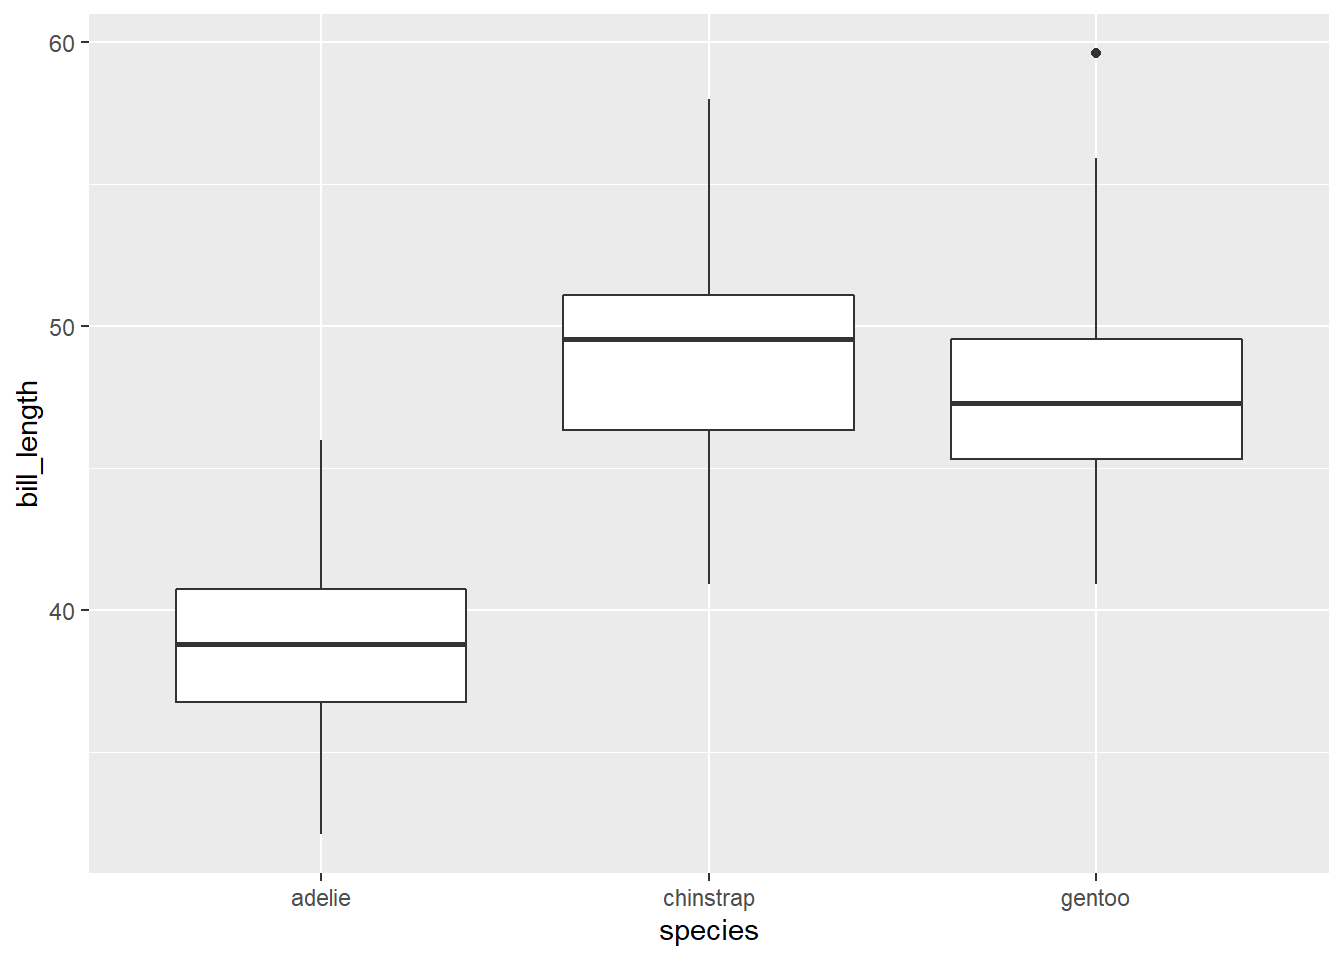
\includegraphics{A-Progessive-Introduction-to-Linear-Models_files/figure-latex/unnamed-chunk-80-1.pdf}

The flipper length and body mass of gentoo penguins tend to be noticeably larger than the other two species, and there is the cluster of gentoo penguis is noticeably different in the plot. Chinstrap and adelie penguins tend to have similar flipper length and body mass, with chinstrap penguins tending to have slightly longer flipper length.

The graphic above can be made better in two ways. 1. Using better colors, and 2. Using more than one visual approach to distinguishing the levels of a \texttt{factor} variable.

Color blindness is a common visual impairment. The colors used above use both red and green, which may be difficult to distinguish. We should use a more friendly color palette. An excellent resource for choosing a color palette is \url{https://colorbrewer2.org} (Brewer (\protect\hyperlink{ref-brewer}{2022})). The webpage allows you to choose a color palette based on certain desired characteristics such as whether the palette is colorblind-friendly, printer friendly, etc. The recommend palettes can be accessed using the \texttt{scale\_color\_brewer} function. We use colorblind-friendly palette below. We also added a few additional customizations below.

\begin{Shaded}
\begin{Highlighting}[]
\NormalTok{gg\_penguin }\SpecialCharTok{+}
  \FunctionTok{geom\_point}\NormalTok{(}\FunctionTok{aes}\NormalTok{(}\AttributeTok{x =}\NormalTok{ body\_mass, }\AttributeTok{y =}\NormalTok{ flipper\_length,}
                 \AttributeTok{color =}\NormalTok{ species, }\AttributeTok{shape =}\NormalTok{ species)) }\SpecialCharTok{+}
  \FunctionTok{scale\_color\_brewer}\NormalTok{(}\AttributeTok{type =} \StringTok{"qual"}\NormalTok{, }\AttributeTok{palette =} \StringTok{"Dark2"}\NormalTok{) }\SpecialCharTok{+}
  \FunctionTok{xlab}\NormalTok{(}\StringTok{"body mass (g)"}\NormalTok{) }\SpecialCharTok{+} \FunctionTok{ylab}\NormalTok{(}\StringTok{"flipper length (mm)"}\NormalTok{) }\SpecialCharTok{+}
  \FunctionTok{ggtitle}\NormalTok{(}\StringTok{"body mass versus flipper length by species"}\NormalTok{)}
\DocumentationTok{\#\# Warning: Removed 2 rows containing missing values}
\DocumentationTok{\#\# (\textasciigrave{}geom\_point()\textasciigrave{}).}
\end{Highlighting}
\end{Shaded}

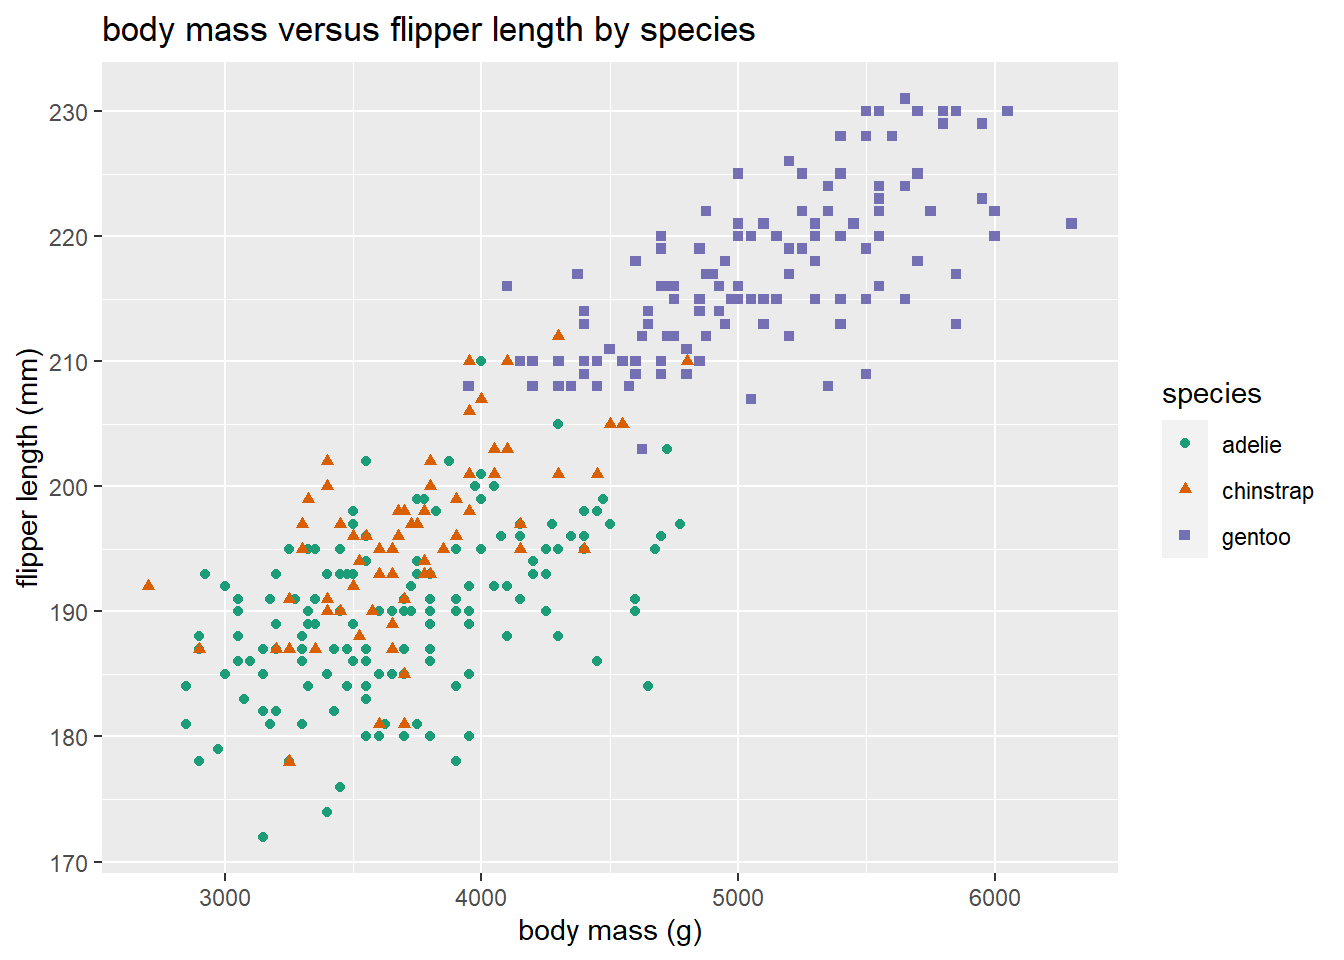
\includegraphics{A-Progessive-Introduction-to-Linear-Models_files/figure-latex/unnamed-chunk-81-1.pdf}

\hypertarget{facetted-plots-and-alternatives}{%
\subsubsection{Facetted plots (and alternatives)}\label{facetted-plots-and-alternatives}}

Facetting creates separate panels (facets) of plots based on one or more facetting variables. The key functions to do this with \textbf{ggplot2} are the \texttt{facet\_grid} and \texttt{facet\_wrap} functions. \texttt{facet\_grid} is used to create a grid of plots based on one or two \texttt{factor} variables, while \texttt{facet\_wrap} wraps facets of panels around the plot. We

Below, we facet scatter plots of \texttt{bill\_length} versus \texttt{bill\_depth} by \texttt{species}.

\begin{Shaded}
\begin{Highlighting}[]
\NormalTok{gg\_penguin }\SpecialCharTok{+}
  \FunctionTok{geom\_point}\NormalTok{(}\FunctionTok{aes}\NormalTok{(}\AttributeTok{x =}\NormalTok{ bill\_depth, }\AttributeTok{y =}\NormalTok{ bill\_length)) }\SpecialCharTok{+}
  \FunctionTok{facet\_grid}\NormalTok{(}\SpecialCharTok{\textasciitilde{}}\NormalTok{ species)}
\DocumentationTok{\#\# Warning: Removed 2 rows containing missing values}
\DocumentationTok{\#\# (\textasciigrave{}geom\_point()\textasciigrave{}).}
\end{Highlighting}
\end{Shaded}

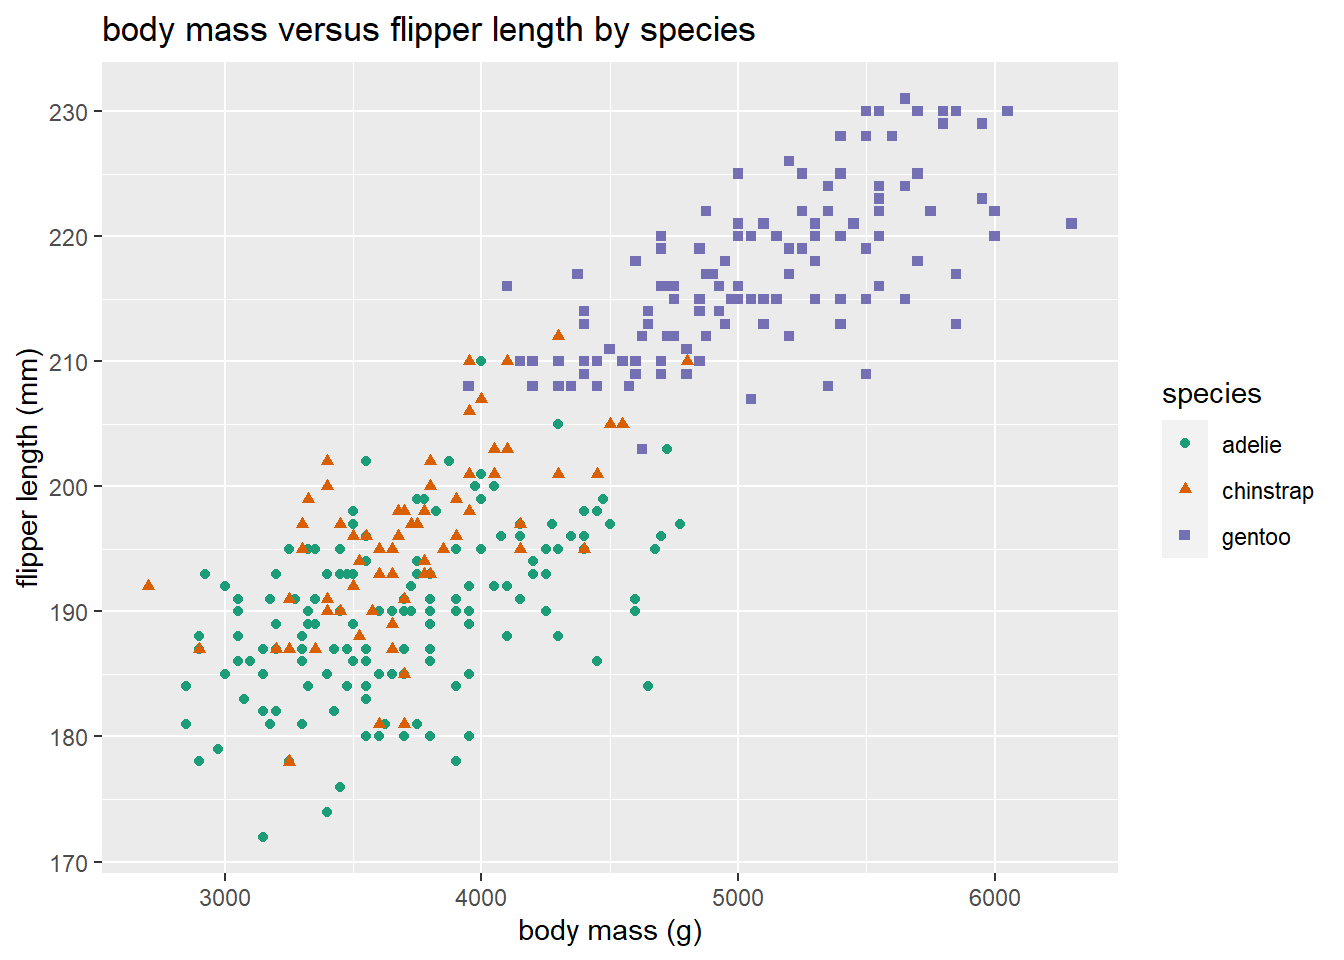
\includegraphics{A-Progessive-Introduction-to-Linear-Models_files/figure-latex/unnamed-chunk-82-1.pdf}

Whereas we previously couldn't discern a relationship between bill length and depth based on a single scatter plot, facetting by \texttt{species} makes it clear there is a positive relationship between \texttt{bill\_length} and \texttt{bill\_depth}. We could have used a group scatter plot for the same thing.

A simpler facetting example would be to facet density plots of \texttt{body\_mass} by \texttt{sex} as shown below.

\begin{Shaded}
\begin{Highlighting}[]
\NormalTok{gg\_penguin }\SpecialCharTok{+} \FunctionTok{geom\_density}\NormalTok{(}\FunctionTok{aes}\NormalTok{(}\AttributeTok{x =}\NormalTok{ body\_mass)) }\SpecialCharTok{+} \FunctionTok{facet\_grid}\NormalTok{(}\SpecialCharTok{\textasciitilde{}}\NormalTok{sex)}
\DocumentationTok{\#\# Warning: Removed 2 rows containing non{-}finite values}
\DocumentationTok{\#\# (\textasciigrave{}stat\_density()\textasciigrave{}).}
\end{Highlighting}
\end{Shaded}

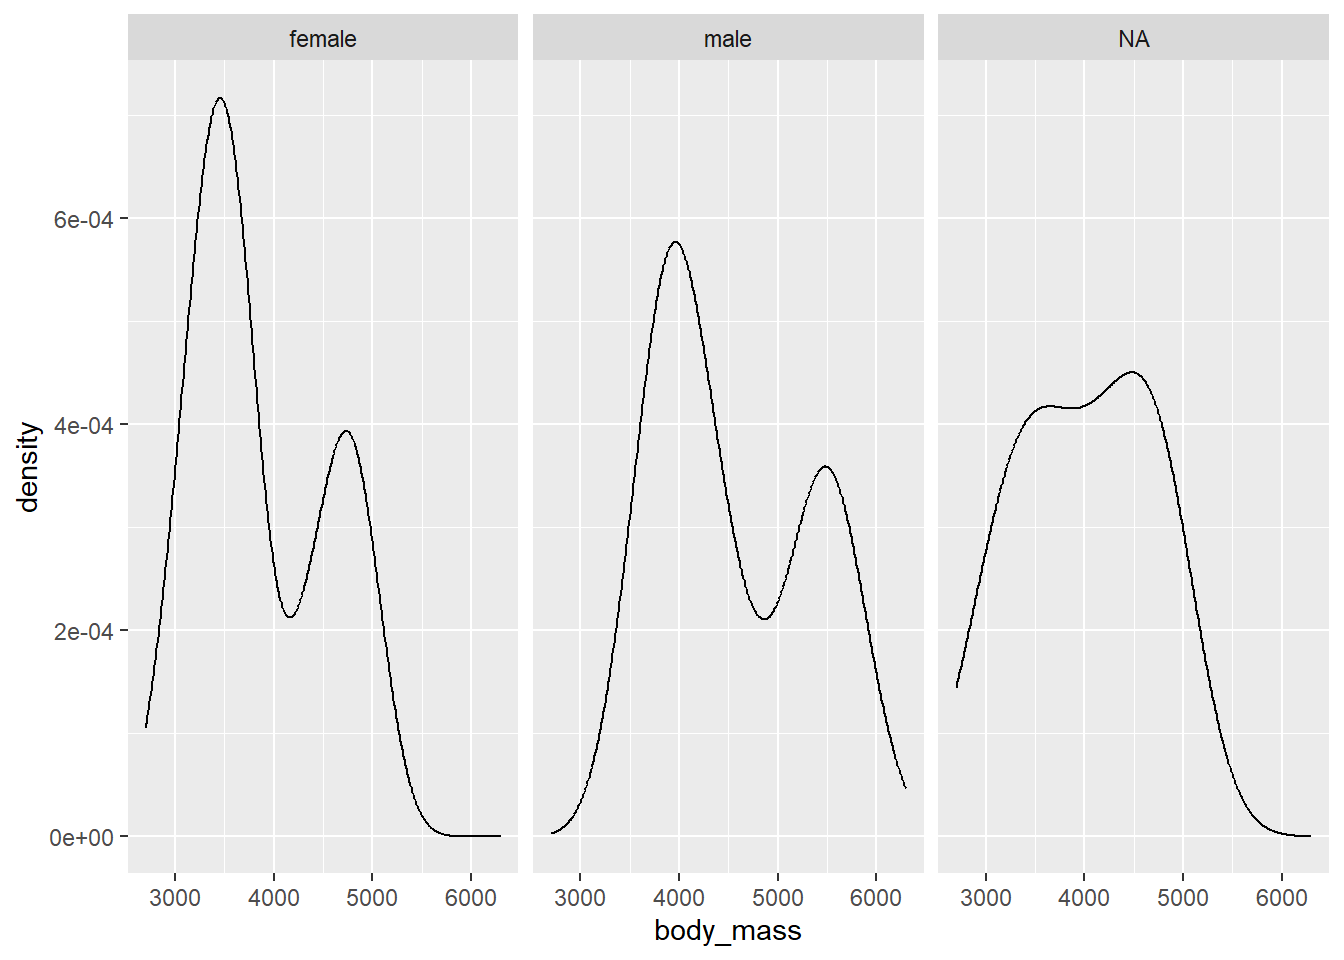
\includegraphics{A-Progessive-Introduction-to-Linear-Models_files/figure-latex/unnamed-chunk-83-1.pdf}

This plot is a bit difficult to interpret. We see that body mass is bimodal for the males and females. Perhaps this is related to \texttt{species}. Since the density plots are in different panels, its a bit tricky to see how they relate to each other. Also, the \texttt{NA} panel is probably not needed.

To get rid of the \texttt{NA} panel, we need to remove all of the observations with \texttt{NA} values. We do this below, using \texttt{subset} to select the desired columns and then using \texttt{na.omit} to remove any rows that have \texttt{NA} values for \texttt{body\_mass}, \texttt{sex}, or \texttt{species}. Note that order matters here because \texttt{na.omit} removes any observation of the data frame that has an \texttt{NA} row. We save the filtered object as \texttt{penguins\_temp}.

\begin{Shaded}
\begin{Highlighting}[]
\NormalTok{penguins\_temp }\OtherTok{\textless{}{-}}
\NormalTok{  penguins\_clean }\SpecialCharTok{|\textgreater{}}
  \FunctionTok{subset}\NormalTok{(}\AttributeTok{select =} \FunctionTok{c}\NormalTok{(body\_mass, sex, species)) }\SpecialCharTok{|\textgreater{}}
  \FunctionTok{na.omit}\NormalTok{()}
\end{Highlighting}
\end{Shaded}

In the next plot, we create density plots of the \texttt{body\_mass} variable. However, we use the \texttt{fill} aesthetic to scale the \texttt{sex} variable so that the we distinguish the densities of male and female penguins with different colors. We set the \texttt{alpha} argument to 0.5 OUTSIDE the \texttt{aes} function (because it is being manually specified) so that the colors are translucent and blend. We also facet by species to see what the patterns look like for the different species.

\begin{Shaded}
\begin{Highlighting}[]
\FunctionTok{ggplot}\NormalTok{(}\AttributeTok{data =}\NormalTok{ penguins\_temp) }\SpecialCharTok{+}
  \FunctionTok{geom\_density}\NormalTok{(}\FunctionTok{aes}\NormalTok{(}\AttributeTok{x =}\NormalTok{ body\_mass, }\AttributeTok{fill =}\NormalTok{ sex), }\AttributeTok{alpha =} \FloatTok{0.5}\NormalTok{) }\SpecialCharTok{+}
  \FunctionTok{facet\_grid}\NormalTok{(}\SpecialCharTok{\textasciitilde{}}\NormalTok{ species)}
\end{Highlighting}
\end{Shaded}

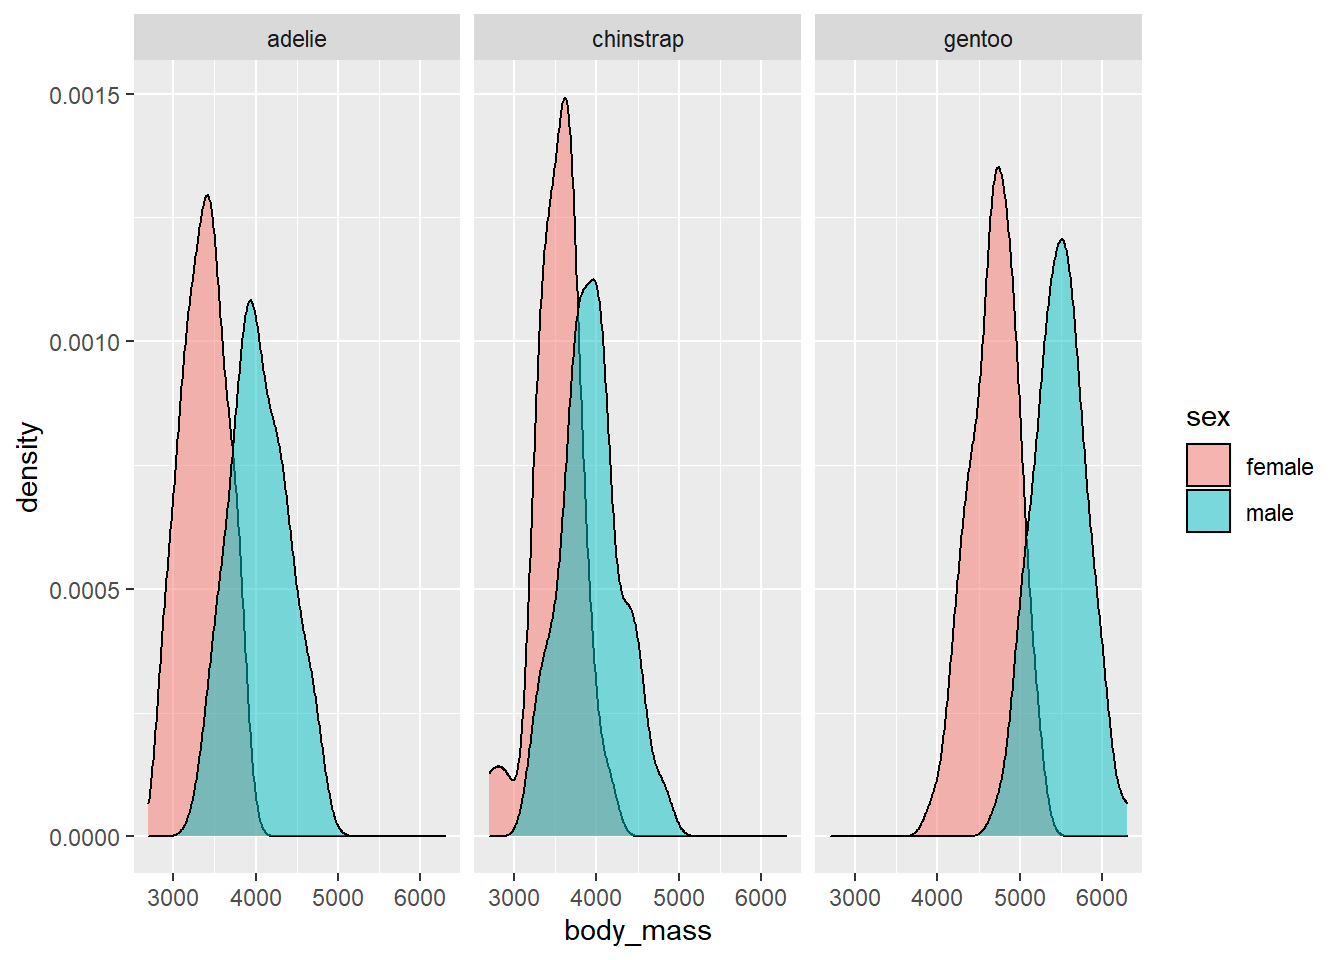
\includegraphics{A-Progessive-Introduction-to-Linear-Models_files/figure-latex/unnamed-chunk-85-1.pdf}

We see that for all species, the body mass of the males tends to be larger than the females.

The examples above provide a small taste of the complicated graphics you can create with \textbf{ggplot2} using only a few lines of code.

\hypertarget{interactive-graphics}{%
\subsubsection{Interactive graphics}\label{interactive-graphics}}

There are many tools for creating interactive graphics in R. We have found the \textbf{\texttt{ggiraph}} package (\protect\hyperlink{ref-R-ggiraph}{Gohel and Skintzos 2023}) useful for creating interactive graphics based on \textbf{ggplot2}. However, it is a bit too complex to discuss here.

The \textbf{\texttt{plotly}} package (\protect\hyperlink{ref-R-plotly}{Sievert et al. 2022}) is an R package to provide the capabilities of plotly \url{https://plotly.com/}, a well-known tool for creating interactive scientific plots. The \texttt{ggplotly} function will instantly make a \texttt{ggplot} interactive (though you may need to customize it for your needs). We provide two examples below.

First, we load the \textbf{\texttt{plotly}} package to have access to the \texttt{ggplotly} function. We then take our previous grouped scatter plot that plotted \texttt{flipper\_length} versus \texttt{body\_mass} distinguishing by \texttt{species} and assign it the name \texttt{ggi}. We then use the \texttt{ggplotly} function in make the graphic interactive. When you hover over a point, the plot interactively provides the exact \texttt{body\_mass} value, \texttt{flipper\_length} value, and \texttt{species} of the observation.

\begin{Shaded}
\begin{Highlighting}[]
\CommentTok{\# load plotly package}
\FunctionTok{library}\NormalTok{(plotly)}
\DocumentationTok{\#\# }
\DocumentationTok{\#\# Attaching package: \textquotesingle{}plotly\textquotesingle{}}
\DocumentationTok{\#\# The following object is masked from \textquotesingle{}package:ggplot2\textquotesingle{}:}
\DocumentationTok{\#\# }
\DocumentationTok{\#\#     last\_plot}
\DocumentationTok{\#\# The following object is masked from \textquotesingle{}package:stats\textquotesingle{}:}
\DocumentationTok{\#\# }
\DocumentationTok{\#\#     filter}
\DocumentationTok{\#\# The following object is masked from \textquotesingle{}package:graphics\textquotesingle{}:}
\DocumentationTok{\#\# }
\DocumentationTok{\#\#     layout}
\CommentTok{\# assign grouped scatter plot name}
\NormalTok{ggi }\OtherTok{\textless{}{-}}
\NormalTok{  gg\_penguin }\SpecialCharTok{+}
  \FunctionTok{geom\_point}\NormalTok{(}\FunctionTok{aes}\NormalTok{(}\AttributeTok{x =}\NormalTok{ body\_mass, }\AttributeTok{y =}\NormalTok{ flipper\_length,}
                 \AttributeTok{color =}\NormalTok{ species, }\AttributeTok{shape =}\NormalTok{ species)) }\SpecialCharTok{+}
  \FunctionTok{scale\_color\_brewer}\NormalTok{(}\AttributeTok{type =} \StringTok{"qual"}\NormalTok{, }\AttributeTok{palette =} \StringTok{"Dark2"}\NormalTok{) }\SpecialCharTok{+}
  \FunctionTok{xlab}\NormalTok{(}\StringTok{"body mass (g)"}\NormalTok{) }\SpecialCharTok{+} \FunctionTok{ylab}\NormalTok{(}\StringTok{"flipper length (mm)"}\NormalTok{) }\SpecialCharTok{+}
  \FunctionTok{ggtitle}\NormalTok{(}\StringTok{"body mass versus flipper length by species"}\NormalTok{)}
\CommentTok{\# make plot interactive}
\FunctionTok{ggplotly}\NormalTok{(ggi)}
\DocumentationTok{\#\# PhantomJS not found. You can install it with webshot::install\_phantomjs(). If it is installed, please make sure the phantomjs executable can be found via the PATH variable.}
\end{Highlighting}
\end{Shaded}

In the next example, we make parallel box plots of \texttt{bill\_length} that distinguish between \texttt{species}.

\begin{Shaded}
\begin{Highlighting}[]
\CommentTok{\# assign parallel box plot name}
\NormalTok{ggi2 }\OtherTok{\textless{}{-}}
\NormalTok{  gg\_penguin }\SpecialCharTok{+}
  \FunctionTok{geom\_boxplot}\NormalTok{(}\FunctionTok{aes}\NormalTok{(}\AttributeTok{x =}\NormalTok{ species, }\AttributeTok{y =}\NormalTok{ bill\_length))}
\CommentTok{\# make plot interactive}
\FunctionTok{ggplotly}\NormalTok{(ggi2)}
\DocumentationTok{\#\# Warning: Removed 2 rows containing non{-}finite values}
\DocumentationTok{\#\# (\textasciigrave{}stat\_boxplot()\textasciigrave{}).}
\end{Highlighting}
\end{Shaded}

The interactive parallel box plot provides information about the box plot of each species (such as the minimum \texttt{bill\_length}, Q1, median, Q3, etc.)

\hypertarget{a-plan-for-data-cleaning-and-exploration}{%
\section{A plan for data cleaning and exploration}\label{a-plan-for-data-cleaning-and-exploration}}

We have provides many examples of data cleaning and exploration using the \texttt{penguins\_raw} data. The analysis above is NOT exhaustive, and there are many additional numeric and visual summaries we could consider. We summarize a basic plan below for initial data cleaning and exploration that we have found useful. You will likely augment this process based on your own preferences and things you learn from the data. We assume you are working with a data frame, which is the most common data structure used for data analysis in R.

\begin{enumerate}
\def\labelenumi{\arabic{enumi}.}
\tightlist
\item
  Import or create the data set.
\item
  Use the \texttt{str} function to get an idea of the initial structure. This can help to identify clear issues you may have had in importing the data, problems with variable names and types, etc.
\item
  Clean the variable names based on your preferences.
\item
  Convert the variables to the appropriate type (e.g., categorical variables to \texttt{factor}).
\item
  Run the \texttt{summary} function on your data frame. Take note of \texttt{NAs}, impossible values that are data entry errors, etc. Perhaps perform some additional cleaning based on this information.
\item
  Compute any additional numeric summaries of the different variables, as desired.
\item
  Create univariate plots of all variables you are considering. Use histograms for discrete \texttt{numeric} variables, density plots for continuous \texttt{numeric} variables, and bar plots for \texttt{factor} variables. Take note of any interesting patterns such as modality, skewness, overall shape, outliers, etc.
\item
  Create bivariate plots of any pairs of variables. Use scatter plots for two \texttt{numeric} variables. Use parallel box plots for \texttt{numeric} and \texttt{factor} variables or perhaps create histogram plots of the \texttt{numeric} variable facetted by the \texttt{factor} variable, or density plots of the \texttt{numeric} variables filled with different colors by the \texttt{factor} variable. Once again, notice any patterns.
\item
  Create multivariate and interactive graphics based on what you learned in the previous steps.
\end{enumerate}

\hypertarget{final-notes-on-missing-or-erroneous-data}{%
\section{Final notes on missing or erroneous data}\label{final-notes-on-missing-or-erroneous-data}}

What should you do with your data when observations are missing information or the information is clearly erroneous?

If the data are clearly erroneous, attempt to get the correct value. If the values cannot be corrected, replace them with \texttt{NA} since you don't have that information.

What should you do about \texttt{NA}s? There are many approaches for dealing with \texttt{NA}s. The proper approach depends a lot on WHY the data are missing. Speaking informally, if there is no systematic reason why the data are missing, then ignoring the observations with missing data isn't a terrible approach. However, if there is a systematic reason why the data are missing (such as individuals not wanting to answer a sensitive question, subjects dying for a specific reason) then ignoring that data can lead to erroneous conclusions.

In what follows, we will generally ignore missing data, assuming the problem is not systematic.

\hypertarget{linear-model-estimation}{%
\chapter{Linear model estimation}\label{linear-model-estimation}}

\hypertarget{a-simple-motivating-example}{%
\section{A simple motivating example}\label{a-simple-motivating-example}}

Suppose we observe data related to the heights of 5 mothers and their adult daughters. The observed heights (measured in inches) are provided in Table \ref{tab:mdheights}. Figure \ref{fig:mdheights-plot} displays a scatter plot of the height data provided in Table \ref{tab:mdheights}. Would it be reasonable to use a mother's height to predict the height of her adult daughter?

\begin{table}

\caption{\label{tab:mdheights}Heights of mothers and their adult daughters (in).}
\centering
\begin{tabular}[t]{rrr}
\toprule
observation & mother's height (in) & daughter's height (in)\\
\midrule
1 & 57.5 & 61.5\\
2 & 60.5 & 63.5\\
3 & 63.5 & 63.5\\
4 & 66.5 & 66.5\\
5 & 69.5 & 66.5\\
\bottomrule
\end{tabular}
\end{table}

\begin{figure}
\centering
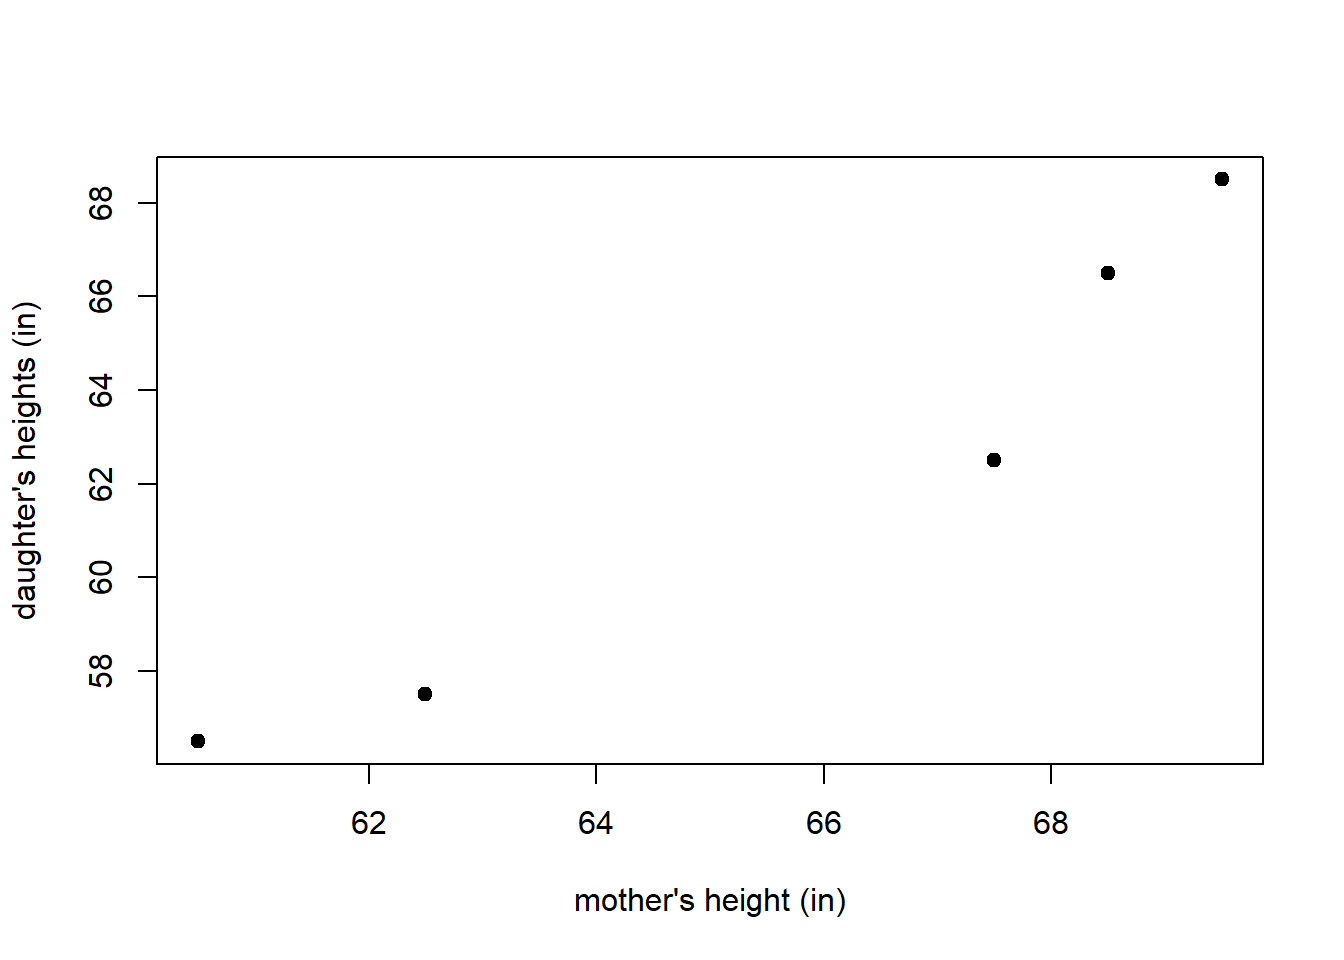
\includegraphics{A-Progessive-Introduction-to-Linear-Models_files/figure-latex/mdheights-plot-1.pdf}
\caption{\label{fig:mdheights-plot}A scatter plot displaying pairs of heights for a mother and her adult daughter.}
\end{figure}

A \textbf{regression analysis} is the process of building a model describing the typical relationship between a set of observed variables. A regression analysis builds the model using observed values of the variables for \(n\) subjects sampled from a population. In the present context, we want to model the height of adult daughters using their height of their mothers. The model we build is known as a \textbf{regression model}.

The variables in a regression analysis may be divided into two types: the response variable and the predictor variables.

The outcome variable we are trying to predict is known as the \textbf{response variable}. Response variables are also known as \textbf{outcome}, \textbf{output}, or \textbf{dependent} variables. The response variable is denoted by \(Y\). The observed value of \(Y\) for observation \(i\) is denoted \(Y_i\).

The variables available to model the response variable are known as \textbf{predictors variables}. Predictor variables are also known as \textbf{explanatory}, \textbf{regressor}, \textbf{input}, \textbf{independent} variables, or simply as \textbf{features}. Following the convention of Weisberg (\protect\hyperlink{ref-alr4}{2014}), we use the term \textbf{regressor} to refer to the variables used in our regression model, whether that is the original predictor variable, some transformation of a predictor, some combination of predictors, etc. Thus, every predictor can be a regressor but not all regressors are a predictor. The regressor variables are denoted as \(X_1, X_2, \ldots, X_{p-1}\). The value of \(X_j\) for observation \(i\) is denoted by \(x_{i,j}\). If there is only a single regressor in the model, we can denote the single regressor as \(X\) and the observed values of \(X\) as \(x_1, x_2, \ldots, x_n\).

For the height data, the 5 pairs of observed data are denoted
\[(x_1, Y_1), (x_2, Y_2), \ldots, (x_5, Y_5),\]
with \((x_i, Y_i)\) denoting the data for observation \(i\). \(x_i\) denotes the mother's height for observation \(i\) and \(Y_i\) denotes the daughter's height for
observation \(i\). Referring to Table \ref{tab:mdheights}, we see that, e.g., \(x_3 = 63.5\) and \(Y_5= 66.5\).

Suppose we want to find the straight line that best fits the plot of mother and daughter heights in Figure \ref{fig:mdheights-plot}. How do we determine the ``best fitting'' model? Consider Figure \ref{fig:two-fitted-lines}, in which 2 potential ``best fitting'' lines are drawn on the scatter plot of the height data. Which one is best?

The rest of this chapter focuses on defining and estimating the parameters of a \emph{linear} regression model. We will start with the simplest type of linear regression, called simple linear regression, which only uses a single regressor variable to model the response. We will then start looking at more complicated linear regression models. After that, we discuss how to evaluate how well an estimated regression model fits the data. We conclude with a summary of some important concepts from the chapter.

\begin{figure}
\centering
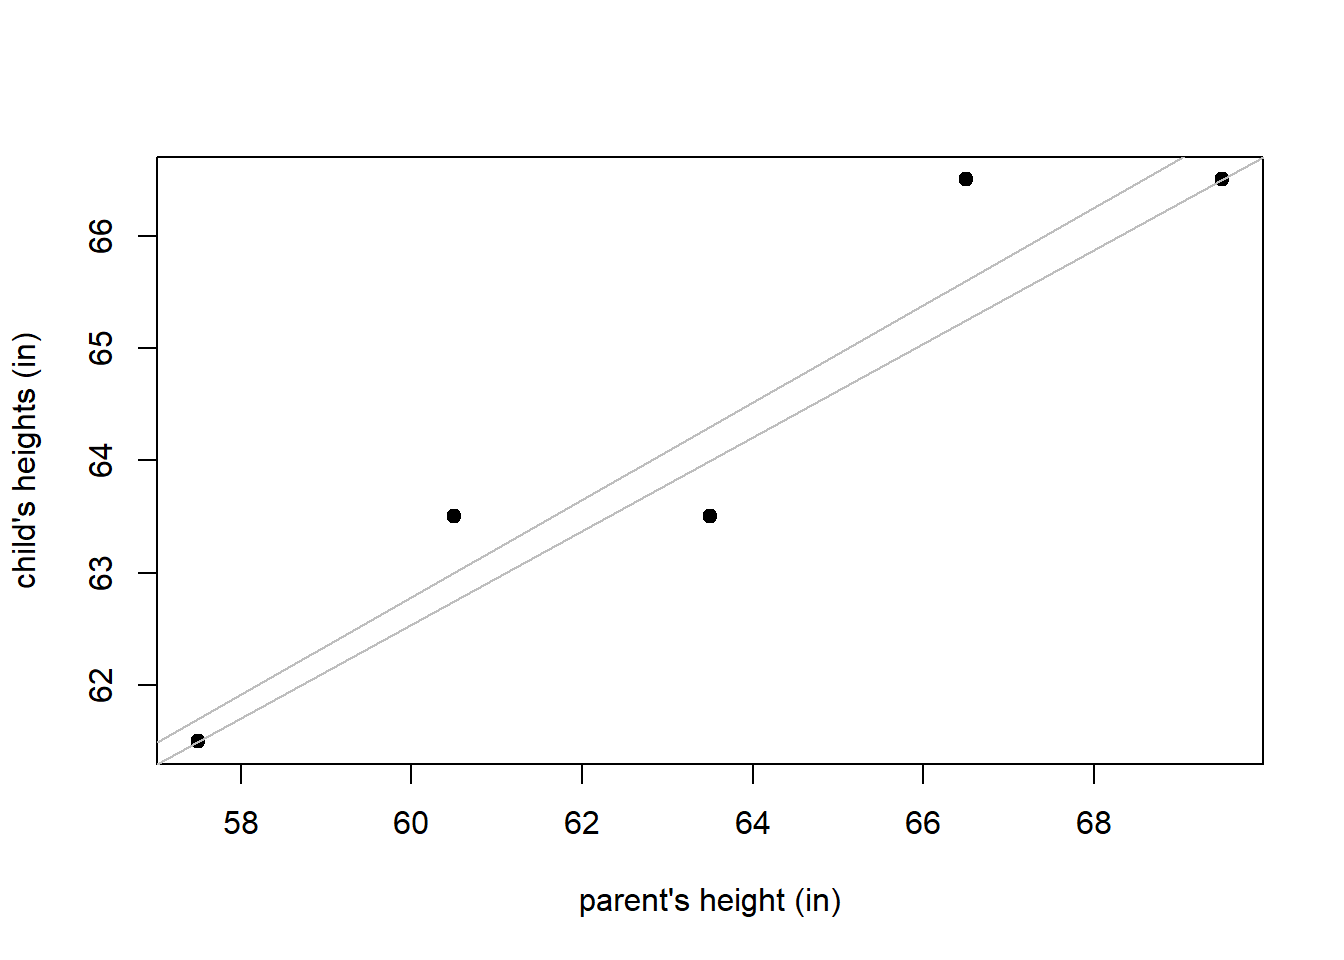
\includegraphics{A-Progessive-Introduction-to-Linear-Models_files/figure-latex/two-fitted-lines-1.pdf}
\caption{\label{fig:two-fitted-lines}Comparison of two potential fitted models to some observed data. The fitted models are shown in grey.}
\end{figure}

\hypertarget{s-slr-estimation}{%
\section{Estimation of the simple linear regression model}\label{s-slr-estimation}}

\textbf{Parameter estimation} is the process of using observed data to estimate parameters of a model. There are many different methods of parameter estimation in statistics: method-of-moments, maximum likelihood, Bayesian, etc. The most common parameter estimation method for linear models is the \textbf{least squares method}, which is commonly called \textbf{Ordinary Least Squares (OLS)} estimation. OLS estimation estimates the regression coefficients with the values that minimize the residual sum of squares (RSS), which we will define shortly.

\hypertarget{ss:fv-resid-rss}{%
\subsection{Model definition, fitted values, residuals, and RSS}\label{ss:fv-resid-rss}}

The regression model for \(Y\) as a function of \(X\), denoted \(E(Y \mid X)\), is the expected value of \(Y\) conditional on the regressor \(X\). Thus, a regression model specifically refers to the expected relationship between the response and regressors.

The \textbf{simple linear regression model} for a response variable assumes the mean of \(Y\) conditional on a single regressor \(X\) is
\[
E(Y\mid X) = \beta_0 + \beta_1 X.
\]

The response variable \(Y\) is modeled as
\[
\begin{aligned}
Y &= E(Y \mid X) + \epsilon \\
&= \beta_0 + \beta_1 X + \epsilon,
\end{aligned}
\label{eq:slr-model-Y}
\]
where \(\epsilon\) is known as the model error.

The error term \(\epsilon\) is literally the deviation of the response variable from its mean.
It is standard to assume that conditional on the regressor variable, the error term has mean 0 and variance \(\sigma^2\), which can be written as
\[
E(\epsilon \mid X) = 0 \label{eq:error-mean}
\]
and
\[
\mathrm{var}(\epsilon \mid X) = \sigma^2.\label{eq:error-var}
\]

Using the response values \(Y_1, \ldots, Y_n\) and their associated regressor values \(x_1, \ldots, x_n\), the observed data are modeled as
\[
\begin{aligned}
Y_i &= \beta_0 + \beta_1 x_i + \epsilon_i \\
&= E(Y\mid X = x_i) + \epsilon_i,
\end{aligned}
\]
for \(i=1\), \(2\),\(\ldots\),\(n\), where \(\epsilon_i\) denotes the error for observation \(i\).

The \textbf{estimated regression model} is defined as
\[\hat{E}(Y|X) = \hat{\beta}_0 + \hat{\beta}_1 X,\]
where \(\hat{\beta}_j\) denotes the estimated value of \(\beta_j\) for \(j=0,1\).

The \(i\)th \textbf{fitted value} is defined as
\[
\hat{Y}_i = \hat{E}(Y|X = x_i) = \hat{\beta}_0 + \hat{\beta}_1 x_i. \label{eq:def-fitted-value-slr}
\]
Thus, the \(i\)th fitted value is the estimated mean of \(Y\) when the regressor \(X=x_i\). More specifically, the \(i\)th fitted value is the estimated mean response based on the regressor value observed for the \(i\)th observation.

The \(i\)th \textbf{residual} is defined as
\[
\hat{\epsilon}_i = Y_i - \hat{Y}_i. \label{eq:def-residual-slr}
\]
The \(i\)th residual is the difference between the response and estimated
mean response of observation \(i\).

The \textbf{residual sum of squares (RSS)} of a regression model is the sum of its squared residuals. The RSS for a simple linear regression model, as a function of the estimated regression coefficients \(\hat{\beta}_0\) and \(\hat{\beta}_1\), is defined as
\[
RSS(\hat{\beta}_0, \hat{\beta}_1) = \sum_{i=1}^n \hat{\epsilon}_i^2. \label{eq:def-rss-slr}
\]

Using the various objects defined above, there are many equivalent expressions for the RSS. Notably, Equation \eqref{eq:def-rss-slr} can be rewritten using Equations \eqref{eq:def-fitted-value-slr} and \eqref{eq:def-residual-slr} as
\[
\begin{aligned}
RSS(\hat{\beta}_0, \hat{\beta}_1) &= \sum_{i=1}^n \hat{\epsilon}_i^2 \\
&= \sum_{i=1}^n (Y_i - \hat{Y}_i)^2 & \\
&= \sum_{i=1}^n (Y_i - \hat{E}(Y|X=x_i))^2 \\
&= \sum_{i=1}^n (Y_i - (\hat{\beta}_0 + \hat{\beta}_1 x_i))^2.
\end{aligned}
\label{eq:equiv-def-rss-slr}
\]

The \textbf{fitted model} is the estimated model that minimizes the RSS and is written as
\[
\hat{Y}=\hat{E}(Y|X) = \hat{\beta}_0 + \hat{\beta}_1 X. \label{eq:def-fitted-model-slr}
\]
Both \(\hat{Y}\) and \(\hat{E}(Y|X)\) are used to denote a fitted model. \(\hat{Y}\) is used for brevity while \(\hat{E}(Y|X)\) is used for clarity. In a simple linear regression context, the fitted model is known as the \textbf{line of best fit}.

In Figure \ref{fig:rss-viz2}, we visualize the response values, fitted values, residuals, and fitted model in a simple linear regression context. Note that:

\begin{itemize}
\tightlist
\item
  The fitted model is shown as the dashed grey line and minimizes the RSS.
\item
  The response values, shown as black dots, are the observed values of \(Y\).
\item
  The fitted values, shown as blue x's, are the values returned by evaluating the fitted
  model at the observed regressor values.
\item
  The residuals, shown as solid orange lines, indicate the distance and direction between the observed responses and their corresponding fitted value. If the response is larger than the fitted value then the residual is positive, otherwise it is negative.
\item
  The RSS is the sum of the squared vertical distances between the response and fitted values.
\end{itemize}

\begin{figure}
\centering
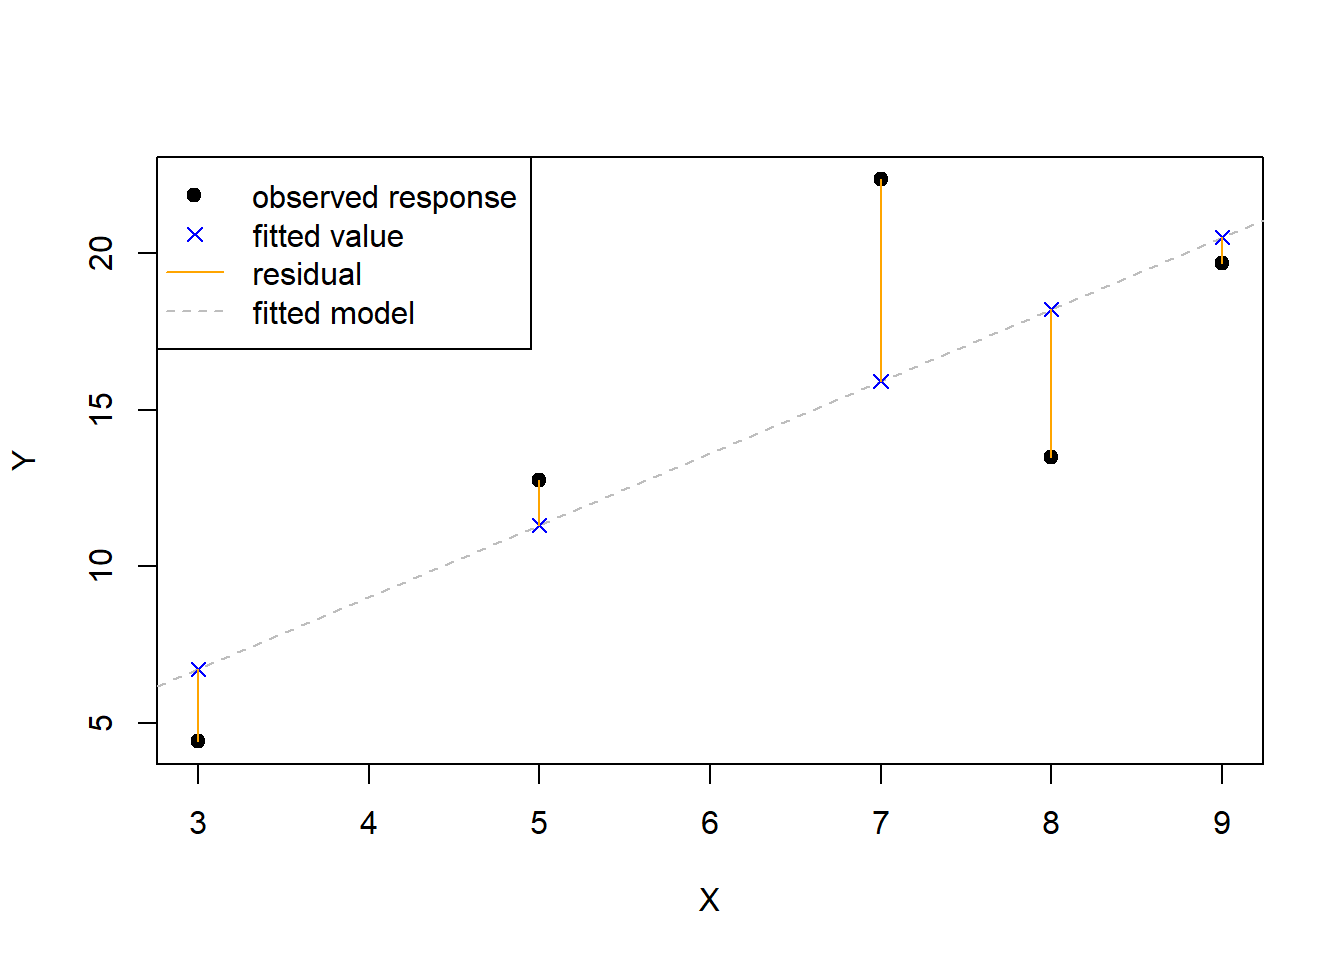
\includegraphics{A-Progessive-Introduction-to-Linear-Models_files/figure-latex/rss-viz2-1.pdf}
\caption{\label{fig:rss-viz2}Visualization of the fitted model, response values, fitted values, and residuals.}
\end{figure}

\hypertarget{ols-estimators-of-the-simple-linear-regression-parameters}{%
\subsection{OLS estimators of the simple linear regression parameters}\label{ols-estimators-of-the-simple-linear-regression-parameters}}

The estimators of \(\beta_0\) and \(\beta_1\) that minimize the RSS for a simple linear regression model can be obtained analytically using basic calculus under minimal assumptions. Specifically, the optimal analytical solutions for \(\hat{\beta}_0\) and \(\hat{\beta}_1\) are valid as long as the regressor values are not a constant value, i.e, \(x_i \neq x_j\) for at least some \(i,j\in \{1,2,\ldots,n\}\).

Define \(\bar{x}=\frac{1}{n}\sum_{i=1}^n x_i\) and
\(\bar{Y} = \frac{1}{n}\sum_{i=1}^n Y_i\). The expression \(\bar{x}\) is read ``x bar'', and it is the sample mean of the observed \(x_i\) values. The OLS estimators of the simple linear regression coefficients that minimize the RSS are
\[
\begin{aligned}
\hat{\beta}_1 &= \frac{\sum_{i=1}^n x_i Y_i - \frac{1}{n} \biggl(\sum_{i=1}^n x_i\biggr)\biggl(\sum_{i=1}^n Y_i\biggr)}{\sum_{i=1}^n x_i^2 - \frac{1}{n} \biggl(\sum_{i=1}^n x_i\biggr)^2} \notag \\
&= \frac{\sum_{i=1}^n (x_i - \bar{x})(Y_i - \bar{Y})}{\sum_{i=1}^n (x_i - \bar{x})^2} \notag \\
&= \frac{\sum_{i=1}^n (x_i - \bar{x})Y_i}{\sum_{i=1}^n (x_i - \bar{x})x_i}
\end{aligned}
\label{eq:slr-beta1hat}
\]
and
\[
\hat{\beta}_0 = \bar{Y} - \hat{\beta}_1 \bar{x}. \label{eq:slr-beta0hat}
\]
The various expressions given in Equation \eqref{eq:slr-beta1hat} are equivalent. In fact, in Equation \eqref{eq:slr-beta1hat}, all of the numerators are equivalent, and all of the denominators are equivalent. We provide derivations of the estimators for \(\hat{\beta}_0\) and \(\hat{\beta}_1\) in Section \ref{slr-derivation}.

In addition to the regression coefficients, the other parameter we mentioned in Section \ref{ss:fv-resid-rss} is the error variance, \(\sigma^2\). The most common estimator of the error variance is
\[
\hat{\sigma}^2 = \frac{RSS}{\mathrm{df}_{RSS}}. \label{eq:sigmasq-hat}
\]
where \(\mathrm{df}_{RSS}\) is the \textbf{degrees of freedom} of the RSS. In a simple linear regression context, the denominator of Equation \eqref{eq:sigmasq-hat} is \(n-2\). See Section \ref{degrees-of-freedom} for more comments about degrees of freedom.

\hypertarget{s:penguins-slr}{%
\section{Penguins simple linear regression example}\label{s:penguins-slr}}

We will use the \texttt{penguins} data set in the \textbf{palmerpenguins} package (\protect\hyperlink{ref-R-palmerpenguins}{Horst, Hill, and Gorman 2022}) to illustrate a very basic simple linear regression analysis.

The \texttt{penguins} data set provides data related to various penguin species measured in the Palmer Archipelago (Antarctica), originally provided by Gorman, Williams, and Fraser (\protect\hyperlink{ref-GormanEtAl2014}{2014}). We start by loading the data into memory.

\begin{Shaded}
\begin{Highlighting}[]
\FunctionTok{data}\NormalTok{(penguins, }\AttributeTok{package =} \StringTok{"palmerpenguins"}\NormalTok{)}
\end{Highlighting}
\end{Shaded}

The data set includes 344 observations of
8 variables. The variables are:

\begin{itemize}
\tightlist
\item
  \texttt{species}: a \texttt{factor} indicating the penguin species.
\item
  \texttt{island}: a \texttt{factor} indicating the island the penguin was observed.
\item
  \texttt{bill\_length\_mm}: a \texttt{numeric} variable indicating the bill length in millimeters.
\item
  \texttt{bill\_depth\_mm}: a \texttt{numeric} variable indicating the bill depth in millimeters.
\item
  \texttt{flipper\_length\_mm}: an \texttt{integer} variable indicating the flipper
  length in millimeters
\item
  \texttt{body\_mass\_g}: an \texttt{integer} variable indicating the body mass in grams.
\item
  \texttt{sex}: a \texttt{factor} indicating the penguin sex (\texttt{female}, \texttt{male}).
\item
  \texttt{year}: an integer denoting the study year the penguin was observed (\texttt{2007}, \texttt{2008}, or \texttt{2009}).
\end{itemize}

We begin by creating a scatter plot of \texttt{bill\_length\_mm} versus \texttt{body\_mass\_g} (y-axis versus x-axis) in Figure \ref{fig:penguin-plot-2}.

\begin{Shaded}
\begin{Highlighting}[]
\FunctionTok{plot}\NormalTok{(bill\_length\_mm }\SpecialCharTok{\textasciitilde{}}\NormalTok{ body\_mass\_g, }\AttributeTok{data =}\NormalTok{ penguins,}
     \AttributeTok{ylab =} \StringTok{"bill length (mm)"}\NormalTok{, }\AttributeTok{xlab =} \StringTok{"body mass (g)"}\NormalTok{,}
     \AttributeTok{main =} \StringTok{"Penguin size measurements"}\NormalTok{)}
\end{Highlighting}
\end{Shaded}

\begin{figure}
\centering
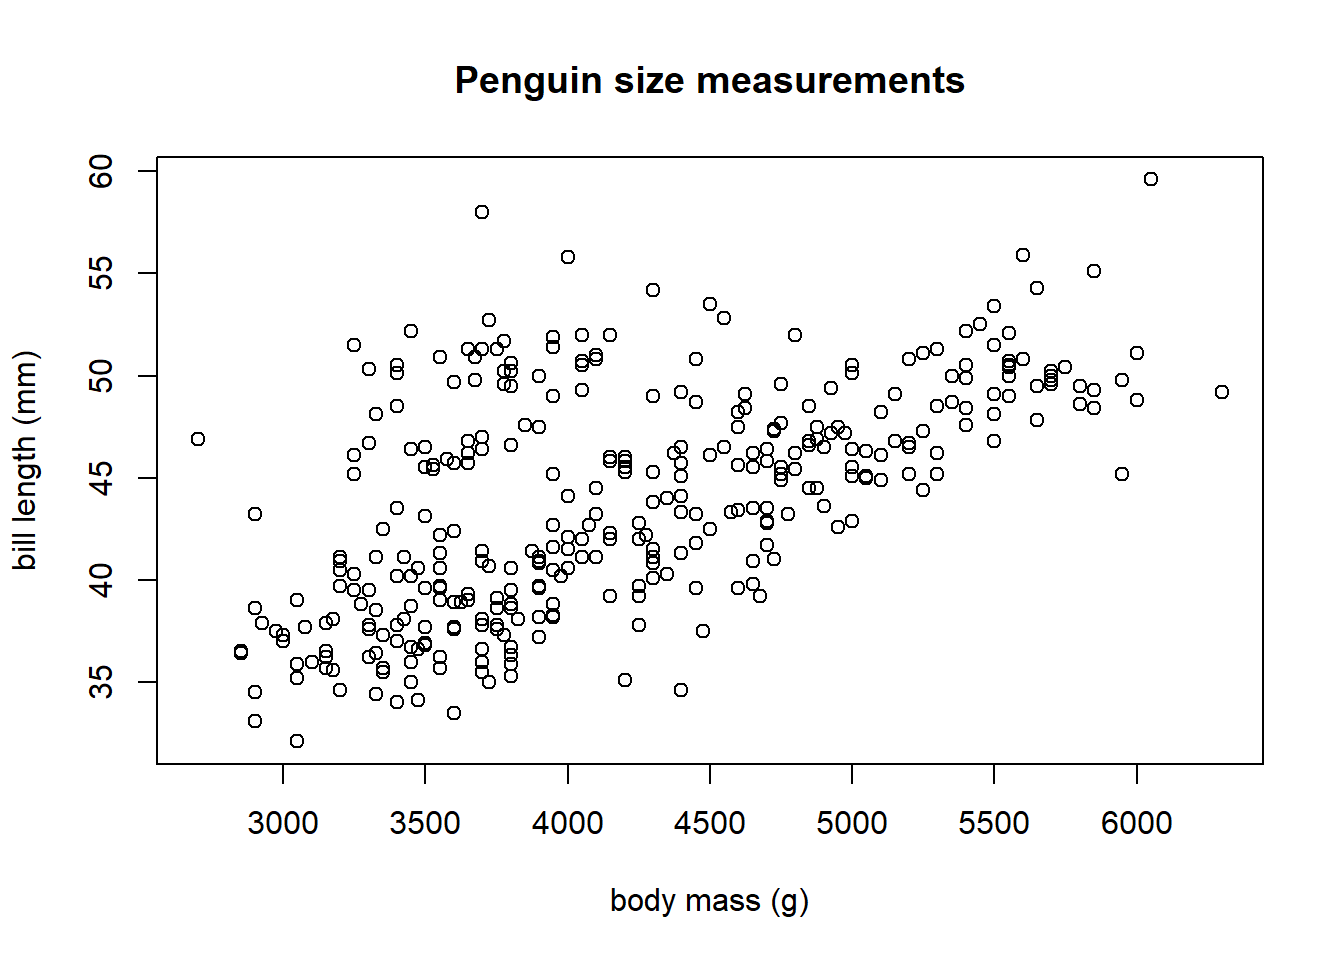
\includegraphics{A-Progessive-Introduction-to-Linear-Models_files/figure-latex/penguin-plot-2-1.pdf}
\caption{\label{fig:penguin-plot-2}A scatter plot of penguin bill length (mm) versus body mass (g)}
\end{figure}

We see a clear positive association between body mass and bill length: as the body mass increases, the bill length tends to increase. The pattern is linear, i.e., roughly a straight line.

We will build a simple linear regression model that regresses \texttt{bill\_length\_mm} on \texttt{body\_mass\_g}. More specifically, we want to estimate the parameters of the regression model \(E(Y\mid X)=\beta_0+\beta_1\,X\), with \(Y=\mathtt{bill\_length\_mm}\) and \(X=\mathtt{body\_mass\_g}\), i.e., we want to estimate the parameters of the model
\[
E(\mathtt{bill\_length\_mm}\mid \mathtt{body\_mass\_g})=\beta_0+\beta_1\,\mathtt{body\_mass\_g}.
\]

The \texttt{lm} function uses OLS estimation to fit a linear model to data. The function has two main arguments:

\begin{itemize}
\tightlist
\item
  \texttt{data}: the data frame in which the model variables are stored. This can be omitted if the variables are already stored in memory.
\item
  \texttt{formula}: a Wilkinson and Rogers (\protect\hyperlink{ref-wilkinsonrogers1973}{1973}) style formula describing the linear regression model. For complete details, run \texttt{?stats::formula} in the Console. If \texttt{y} is the response variable and \texttt{x} is an available numeric predictor, then \texttt{formula\ =\ y\ \textasciitilde{}\ x} tells \texttt{lm} to fit the simple linear regression model \(E(Y|X)=\beta_0+\beta_1 X\).
\end{itemize}

We use the code below to fit a linear model regressing \texttt{bill\_length\_mm} on \texttt{body\_mass\_g} using the \texttt{penguins} data frame and assign the result the name \texttt{lmod}. \texttt{lmod} is an object of class \texttt{lm}.

\begin{Shaded}
\begin{Highlighting}[]
\NormalTok{lmod }\OtherTok{\textless{}{-}} \FunctionTok{lm}\NormalTok{(bill\_length\_mm }\SpecialCharTok{\textasciitilde{}}\NormalTok{ body\_mass\_g, }\AttributeTok{data =}\NormalTok{ penguins) }\CommentTok{\# fit model}
\FunctionTok{class}\NormalTok{(lmod) }\CommentTok{\# class of lmod}
\DocumentationTok{\#\# [1] "lm"}
\end{Highlighting}
\end{Shaded}

The \texttt{summary} function is commonly used to summarize the results of our fitted model. When an \texttt{lm} object is supplied to the \texttt{summary} function, it returns:

\begin{itemize}
\tightlist
\item
  \texttt{Call}: the function call used to fit the model.
\item
  \texttt{Residuals}: A 5-number summary of the \(\hat{\epsilon}_1, \ldots, \hat{\epsilon}_n\).
\item
  \texttt{Coefficients}: A table that lists:

  \begin{itemize}
  \tightlist
  \item
    The regressors in the fitted model.
  \item
    \texttt{Estimate}: the estimated coefficient for each regressor.
  \item
    \texttt{Std.\ Error}: the \emph{estimated} standard error of the estimated coefficients.
  \item
    \texttt{t\ value}: the computed test statistic associated with testing \(H_0: \beta_j = 0\) versus \(H_a: \beta_j \neq 0\) for each regression coefficient in the model.
  \item
    \texttt{Pr(\textgreater{}\textbar{}t\textbar{})}: the associated p-value of each test.
  \end{itemize}
\item
  Various summary statistics:

  \begin{itemize}
  \tightlist
  \item
    \texttt{Residual\ standard\ error} is the value of \(\hat{\sigma}\), the estimate of the error standard deviation. The degrees of freedom is \(\mathrm{df}_{RSS}\), the number of observations minus the number of estimated coefficients in the model.
  \item
    \texttt{Multiple\ R-squared} is an estimate of model fit discussed in Section \ref{evaluating-model-fit}.
  \item
    \texttt{Adjusted\ R-squared} is a modified version of \texttt{Multiple\ R-squared}.
  \item
    \texttt{F-statistic} is the test statistic for the test that compares the model with an only an intercept to the fitted model. The \texttt{DF} (degrees of freedom) values relate to the statistic under the null hypothesis, and the \texttt{p-value} is the p-value for the test.
  \end{itemize}
\end{itemize}

We use the \texttt{summary} function on \texttt{lmod} to produce the output below.

\begin{Shaded}
\begin{Highlighting}[]
\CommentTok{\# summarize results stored in lmod}
\FunctionTok{summary}\NormalTok{(lmod)}
\DocumentationTok{\#\# }
\DocumentationTok{\#\# Call:}
\DocumentationTok{\#\# lm(formula = bill\_length\_mm \textasciitilde{} body\_mass\_g, data = penguins)}
\DocumentationTok{\#\# }
\DocumentationTok{\#\# Residuals:}
\DocumentationTok{\#\#      Min       1Q   Median       3Q      Max }
\DocumentationTok{\#\# {-}10.1251  {-}3.0434  {-}0.8089   2.0711  16.1109 }
\DocumentationTok{\#\# }
\DocumentationTok{\#\# Coefficients:}
\DocumentationTok{\#\#              Estimate Std. Error t value Pr(\textgreater{}|t|)    }
\DocumentationTok{\#\# (Intercept) 2.690e+01  1.269e+00   21.19   \textless{}2e{-}16 ***}
\DocumentationTok{\#\# body\_mass\_g 4.051e{-}03  2.967e{-}04   13.65   \textless{}2e{-}16 ***}
\DocumentationTok{\#\# {-}{-}{-}}
\DocumentationTok{\#\# Signif. codes:  }
\DocumentationTok{\#\# 0 \textquotesingle{}***\textquotesingle{} 0.001 \textquotesingle{}**\textquotesingle{} 0.01 \textquotesingle{}*\textquotesingle{} 0.05 \textquotesingle{}.\textquotesingle{} 0.1 \textquotesingle{} \textquotesingle{} 1}
\DocumentationTok{\#\# }
\DocumentationTok{\#\# Residual standard error: 4.394 on 340 degrees of freedom}
\DocumentationTok{\#\#   (2 observations deleted due to missingness)}
\DocumentationTok{\#\# Multiple R{-}squared:  0.3542, Adjusted R{-}squared:  0.3523 }
\DocumentationTok{\#\# F{-}statistic: 186.4 on 1 and 340 DF,  p{-}value: \textless{} 2.2e{-}16}
\end{Highlighting}
\end{Shaded}

Using the output above, we see that the estimated parameters are \(\hat{\beta}_0=26.9\) and \(\hat{\beta}_1=0.004\). Thus, our fitted model is
\[
\widehat{\mathtt{bill\_length\_mm}}=26.9+0.004 \,\mathtt{body\_mass\_g}.
\]

In the context of a simple linear regression model, the intercept term is the expected response when the value of the regressor is zero, while the slope is the expected change in the response when the regressor increases by 1 unit. Thus, based on the model we fit to the \texttt{penguins} data, we can make the following interpretations:

\begin{itemize}
\tightlist
\item
  \(\hat{\beta}_1\): If a penguin has a body mass 1 gram larger than another penguin, we expect the larger penguin's bill length to be 0.004 millimeters longer.
\item
  \(\hat{\beta}_0\): A penguin with a body mass of 0 grams is expected to have a bill length of 26.9 millimeters.
\end{itemize}

The latter interpretation is nonsensical. It doesn't make sense to discuss a penguin with a body mass of 0 grams unless we are talking about an embryo, in which case it doesn't even make sense to discuss bill length. This is caused by the fact that we are extrapolating far outside the observed body mass values. Our data only includes information for adult penguins, so we should be cautious about drawing conclusions for penguins at other life stages.

The \texttt{abline} function can be used to automatically overlay the fitted model on the observed data. We run the code below to produce Figure \ref{fig:slr-penguin-fit}. The fit of the model to our observed data seems reasonable.

\begin{Shaded}
\begin{Highlighting}[]
\FunctionTok{plot}\NormalTok{(bill\_length\_mm }\SpecialCharTok{\textasciitilde{}}\NormalTok{ body\_mass\_g, }\AttributeTok{data =}\NormalTok{ penguins, }\AttributeTok{main =} \StringTok{"Penguin size measurements"}\NormalTok{,}
     \AttributeTok{ylab =} \StringTok{"bill length (mm)"}\NormalTok{, }\AttributeTok{xlab =} \StringTok{"body mass (g)"}\NormalTok{)}
\CommentTok{\# draw fitted line of plot}
\FunctionTok{abline}\NormalTok{(lmod)}
\end{Highlighting}
\end{Shaded}

\begin{figure}
\centering
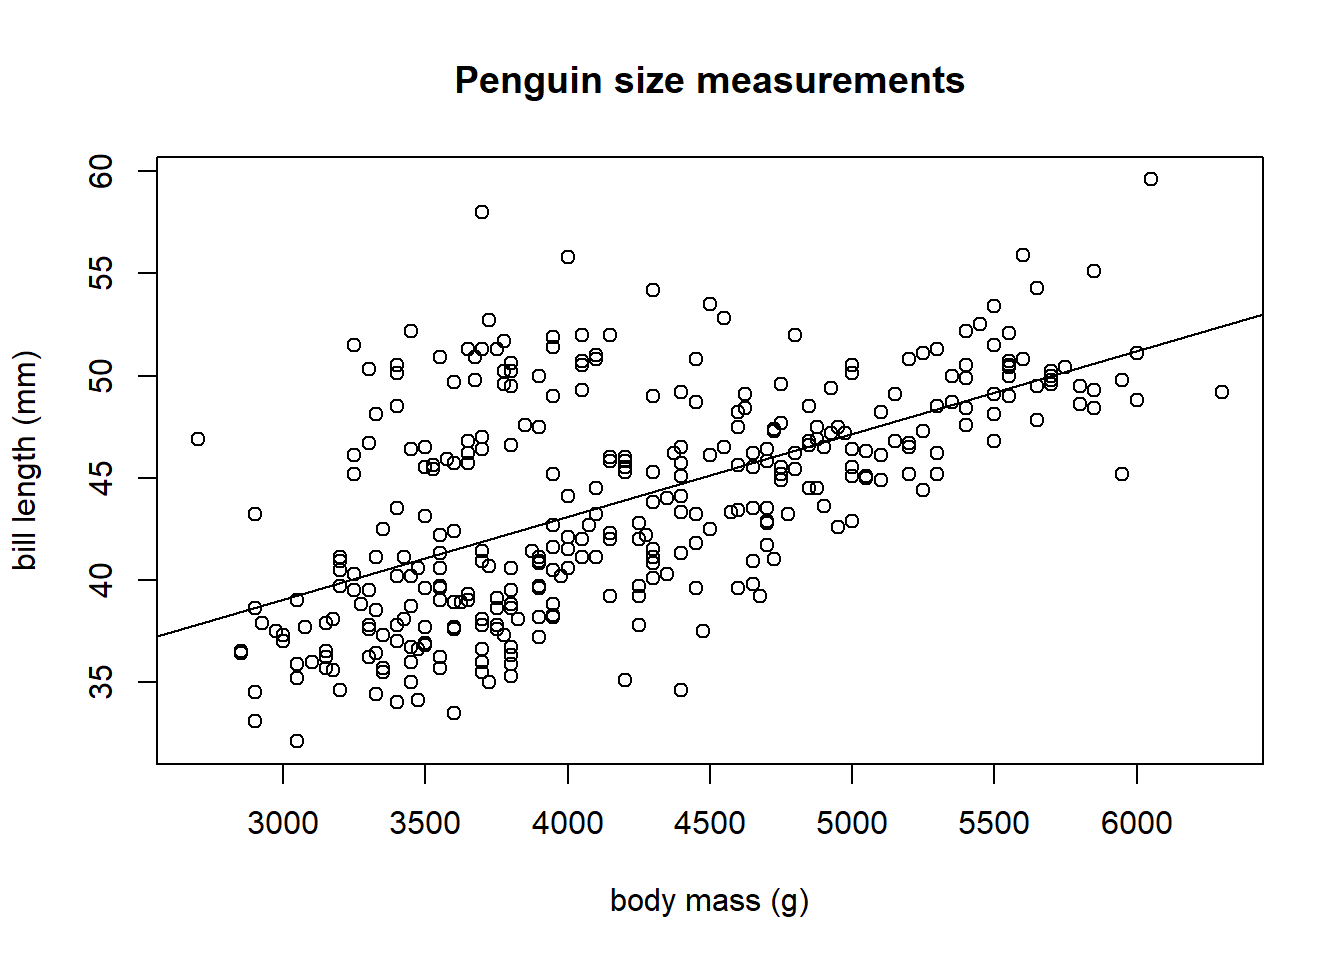
\includegraphics{A-Progessive-Introduction-to-Linear-Models_files/figure-latex/slr-penguin-fit-1.pdf}
\caption{\label{fig:slr-penguin-fit}The fitted model overlaid on the penguin data.}
\end{figure}

R provides many additional methods (generic functions that do something specific when applied to a certain type of object) for \texttt{lm} objects. Commonly used ones include:

\begin{itemize}
\tightlist
\item
  \texttt{residuals}: extracts the residuals, \(\hat{\epsilon}_1, \ldots, \hat{\epsilon}_n\) from an \texttt{lm} object.
\item
  \texttt{fitted}: extracts the fitted values, \(\hat{Y}_1, \ldots, \hat{Y}_n\) from an \texttt{lm} object.
\item
  \texttt{predict}: by default, computes \(\hat{Y}_1, \ldots, \hat{Y}_n\) for an \texttt{lm} object. It can also be used to make arbitrary predictions for the \texttt{lm} object.
\item
  \texttt{coef} or \texttt{coefficients}: extracts the estimated coefficients from an \texttt{lm} object.
\item
  \texttt{deviance}: extracts the RSS from an \texttt{lm} object.
\item
  \texttt{df.residual}: extracts \(\mathrm{df}_{RSS}\), the degrees of freedom for the RSS, from an \texttt{lm} object.
\item
  \texttt{sigma}: extracts \(\hat{\sigma}\) from an \texttt{lm} object.
\end{itemize}

We now use some of the methods to extract important characteristics of our fitted model.

We extract the estimated regression coefficients, \(\hat{\beta}_0\) and \(\hat{\beta}_1\), using the \texttt{coef} function.

\begin{Shaded}
\begin{Highlighting}[]
\NormalTok{(coeffs }\OtherTok{\textless{}{-}} \FunctionTok{coef}\NormalTok{(lmod)) }\CommentTok{\# extract, assign, and print coefficients}
\DocumentationTok{\#\#  (Intercept)  body\_mass\_g }
\DocumentationTok{\#\# 26.898872424  0.004051417}
\end{Highlighting}
\end{Shaded}

We extract the vector of residuals, \(\hat{\epsilon}_1,\ldots, \hat{\epsilon}_n\), using the \texttt{residuals} function.

\begin{Shaded}
\begin{Highlighting}[]
\NormalTok{ehat }\OtherTok{\textless{}{-}} \FunctionTok{residuals}\NormalTok{(lmod) }\CommentTok{\# extract and assign residuals}
\FunctionTok{head}\NormalTok{(ehat) }\CommentTok{\# first few residuals}
\DocumentationTok{\#\#          1          2          3          5          6 }
\DocumentationTok{\#\# {-}2.9916846 {-}2.7942554  0.2340237 {-}4.1762596 {-}2.3865430 }
\DocumentationTok{\#\#          7 }
\DocumentationTok{\#\# {-}2.6852575}
\end{Highlighting}
\end{Shaded}

We extract the vector of fitted values, \(\hat{Y}_1,\ldots, \hat{Y}_n\), using the \texttt{fitted} function.

\begin{Shaded}
\begin{Highlighting}[]
\NormalTok{yhat }\OtherTok{\textless{}{-}} \FunctionTok{fitted}\NormalTok{(lmod) }\CommentTok{\# extract and assign fitted values}
\FunctionTok{head}\NormalTok{(yhat) }\CommentTok{\# first few fitted values}
\DocumentationTok{\#\#        1        2        3        5        6        7 }
\DocumentationTok{\#\# 42.09168 42.29426 40.06598 40.87626 41.68654 41.58526}
\end{Highlighting}
\end{Shaded}

We can also extract the vector of fitted values using the \texttt{predict} function.

\begin{Shaded}
\begin{Highlighting}[]
\NormalTok{yhat2 }\OtherTok{\textless{}{-}} \FunctionTok{predict}\NormalTok{(lmod) }\CommentTok{\# compute and assign fitted values}
\FunctionTok{head}\NormalTok{(yhat2) }\CommentTok{\# first few fitted values}
\DocumentationTok{\#\#        1        2        3        5        6        7 }
\DocumentationTok{\#\# 42.09168 42.29426 40.06598 40.87626 41.68654 41.58526}
\end{Highlighting}
\end{Shaded}

We extract the RSS of the model using the \texttt{deviance} function.

\begin{Shaded}
\begin{Highlighting}[]
\NormalTok{(rss }\OtherTok{\textless{}{-}} \FunctionTok{deviance}\NormalTok{(lmod)) }\CommentTok{\# extract, assign, and print rss}
\DocumentationTok{\#\# [1] 6564.494}
\end{Highlighting}
\end{Shaded}

We extract the residual degrees of freedom using the \texttt{df.residual} function.

\begin{Shaded}
\begin{Highlighting}[]
\NormalTok{(dfr }\OtherTok{\textless{}{-}} \FunctionTok{df.residual}\NormalTok{(lmod)) }\CommentTok{\# extract n {-} p}
\DocumentationTok{\#\# [1] 340}
\end{Highlighting}
\end{Shaded}

We extract the estimated error standard deviation, \(\hat{\sigma}=\sqrt{\hat{\sigma}^2}\), using the \texttt{sigma} function. In the code below, we square \(\hat{\sigma}\) to estimate the error variance, \(\hat{\sigma}^2\).

\begin{Shaded}
\begin{Highlighting}[]
\NormalTok{(sigmasqhat }\OtherTok{\textless{}{-}} \FunctionTok{sigma}\NormalTok{(lmod)}\SpecialCharTok{\^{}}\DecValTok{2}\NormalTok{) }\CommentTok{\# estimated error variance}
\DocumentationTok{\#\# [1] 19.30734}
\end{Highlighting}
\end{Shaded}

From the output above, we that the the first 3 residuals are -2.99, -2.79, and 0.23. The first 3 fitted values are 42.09, 42.29, and 40.07. The RSS for the fitted model is 6564.49 with 340 degrees of freedom. The estimated error variance, \(\hat{\sigma}^2\), is 19.31.

We use the \texttt{methods} function to obtain a full list of methods available for \texttt{lm} objects using the code below.

\begin{Shaded}
\begin{Highlighting}[]
\FunctionTok{methods}\NormalTok{(}\AttributeTok{class =} \StringTok{"lm"}\NormalTok{)}
\DocumentationTok{\#\#  [1] add1           alias          anova         }
\DocumentationTok{\#\#  [4] case.names     coerce         confint       }
\DocumentationTok{\#\#  [7] cooks.distance deviance       dfbeta        }
\DocumentationTok{\#\# [10] dfbetas        drop1          dummy.coef    }
\DocumentationTok{\#\# [13] effects        extractAIC     family        }
\DocumentationTok{\#\# [16] formula        fortify        hatvalues     }
\DocumentationTok{\#\# [19] influence      initialize     kappa         }
\DocumentationTok{\#\# [22] labels         logLik         model.frame   }
\DocumentationTok{\#\# [25] model.matrix   nobs           plot          }
\DocumentationTok{\#\# [28] predict        print          proj          }
\DocumentationTok{\#\# [31] qr             residuals      rstandard     }
\DocumentationTok{\#\# [34] rstudent       show           simulate      }
\DocumentationTok{\#\# [37] slotsFromS3    summary        variable.names}
\DocumentationTok{\#\# [40] vcov          }
\DocumentationTok{\#\# see \textquotesingle{}?methods\textquotesingle{} for accessing help and source code}
\end{Highlighting}
\end{Shaded}

\hypertarget{defining-a-linear-model}{%
\section{Defining a linear model}\label{defining-a-linear-model}}

\hypertarget{ss-necessary-components}{%
\subsection{Necessary components and notation}\label{ss-necessary-components}}

We now wish to discuss linear models in a broader context. We begin by defining notation for the components of a linear model and provide some of their important properties. We repeat some of the previous discussion for clarity.

\begin{itemize}
\tightlist
\item
  \(Y\) denotes the response variable.

  \begin{itemize}
  \tightlist
  \item
    The response variable is treated as a random variable.
  \item
    We will observe realizations of this random variable for each observation in our data set.
  \end{itemize}
\item
  \(X\) denotes a single regressor variable. \(X_1, X_2, \ldots, X_{p-1}\) denote distinct regressor variables if we are performing regression with multiple regressor variables.

  \begin{itemize}
  \tightlist
  \item
    The regressor variables are treated as non-random variables.
  \item
    The observed values of the regressor variables are treated as fixed, known values.
  \end{itemize}
\item
  \(\mathbb{X}=\{X_0, X_1,\ldots,X_{p-1}\}\) denotes the collection of all regressors under consideration, though this notation is really only needed in the context of multiple regression. \(X_0\) is usually the constant regressor 1, which is needed to include an intercept in the regression model.
\item
  \(\beta_0\), \(\beta_1\), \(\ldots\), \(\beta_{p-1}\) denote \textbf{regression coefficients}.

  \begin{itemize}
  \tightlist
  \item
    Regression coefficients are statistical parameters that we will estimate from our data.
  \item
    The regression coefficients are treated as fixed, non-random but unknown values.
  \item
    Regression coefficients are not observable.
  \end{itemize}
\item
  \(\epsilon\) denotes model \textbf{error}.

  \begin{itemize}
  \tightlist
  \item
    The model error is more accurately described as random variation of each observation from the regression model.
  \item
    The error is treated as a random variable.
  \item
    The error is assumed to have mean 0 for all values of the regressors. We write this as \(E(\epsilon \mid \mathbb{X}) = 0\), which is read as, ``The expected value of \(\epsilon\) conditional on knowing all the regressor values equals 0''. The notation ``\(\mid \mathbb{X}\)'' extends the notation used in Equation \eqref{eq:slr-equation} to multiple regressors.
  \item
    The variance of the errors is assumed to be a constant value for all values of the regressors. We write this assumption as \(\mathrm{var}(\epsilon \mid \mathbb{X})=\sigma^2\).
  \item
    The error is never observable (except in the context of a simulation study where the experimenter literally defines the true model).
  \end{itemize}
\end{itemize}

\hypertarget{standard-definition-of-linear-model}{%
\subsection{Standard definition of linear model}\label{standard-definition-of-linear-model}}

In general, a linear regression model can have an arbitrary number of regressors. A \textbf{multiple linear regression} model has two or more regressors.

A \textbf{linear model} for \(Y\) is defined by the equation
\[
\begin{aligned}
Y &= \beta_0 + \beta_1 X_1 + \beta_2 X_2 + \cdots + \beta_{p-1}
X_{p-1} + \epsilon \\
&= E(Y \mid \mathbb{X}) + \epsilon.
\end{aligned}
\label{eq:lmdef}
\]

We write the linear model in this way to emphasize the fact \emph{the response value equals the expected response for that combination of regressor values plus some error}. It should be clear from comparing Equation \eqref{eq:lmdef} with the previous line that
\[
E(Y \mid \mathbb{X}) = \beta_0 + \beta_1 X_1 + \beta_2 X_2 + \cdots + \beta_{p-1} X_{p-1},
\]
which we prove in Chapter \ref{linear-model-theory}.

More generally, one can say that a regression model is linear if the mean function can be written as a linear combination of the regression coefficients and known values created from our regressor variables, i.e.,
\[
E(Y \mid \mathbb{X}) = \sum_{j=0}^{p-1} c_j \beta_j, \label{eq:lmdef-cj}
\]
where \(c_0, c_1, \ldots, c_{p-1}\) are known functions of
the regressor variables, e.g., \(c_1 = X_1 X_2 X_3\), \(c_3 = X_2^2\),
\(c_8 = \ln(X_1)/X_2^2\), etc. Thus, if \(g_0,\ldots,g_{p-1}\) are functions of \(\mathbb{X}\), then we can say that the regression model is linear if
it can be written as
\[
E(Y\mid \mathbb{X}) = \sum_{j=0}^{p-1} g_j(\mathbb{X})\beta_j.
\]

A model is linear because of its \emph{form}, not the shape it produces. Many of the linear model examples given below do not result in a straight line or surface, but are curved. Some examples of linear regression models are:

\begin{itemize}
\tightlist
\item
  \(E(Y|X) = \beta_0\).
\item
  \(E(Y|X) = \beta_0 + \beta_1 X + \beta_2 X^2\).
\item
  \(E(Y|X_1, X_2) = \beta_0 + \beta_1 X_1 + \beta_2 X_2\).
\item
  \(E(Y|X_1, X_2) = \beta_0 + \beta_1 X_1 + \beta_2 X_2 + \beta_3 X_1 X_2\).
\item
  \(E(Y|X_1, X_2) = \beta_0 + \beta_1 \ln(X_1) + \beta_2 X_2^{-1}\).
\item
  \(E(\ln(Y)|X_1, X_2) = \beta_0 + \beta_1 X_1 + \beta_2 X_2\).
\item
  \(E(Y^{-1}|X_1, X_2) = \beta_0 + \beta_1 X_1 + \beta_2 X_2\).
\end{itemize}

Some examples of non-linear regression models are:

\begin{itemize}
\tightlist
\item
  \(E(Y|X) = \beta_0 + e^{\beta_1 X}\).
\item
  \(E(Y|X) = \beta_0 + \beta_1 X/(\beta_2 + X)\).
\end{itemize}

The latter regression models are non-linear models because there is no way to express them using the expression in Equation \eqref{eq:lmdef-cj}.

\hypertarget{estimation-of-the-multiple-linear-regression-model}{%
\section{Estimation of the multiple linear regression model}\label{estimation-of-the-multiple-linear-regression-model}}

Suppose we want to estimate the parameters of a linear model with 1 or more regressors, i.e., when we use the model
\[
Y=\beta_0 + \beta_1 X_1 + \cdots + \beta_{p-1} X_{p-1} + \epsilon.
\]

The system of equations relating the responses, the regressors, and the errors for all \(n\) observations can be written as
\[
Y_i = \beta_0 + \beta_1 x_{i,1} + \beta_2 x_{i,2} + \cdots + \beta_{p-1} x_{i,p-1} + \epsilon_i,\quad i=1,2,\ldots,n.
\label{eq:lmSystem}
\]

\hypertarget{using-matrix-notation-to-represent-a-linear-model}{%
\subsection{Using matrix notation to represent a linear model}\label{using-matrix-notation-to-represent-a-linear-model}}

We can simplify the linear model described in Equation \eqref{eq:lmSystem} using matrix notation. It may be useful to refer to Appendix \ref{overview-of-matrix-facts} for a brief overview of matrix-related information.

We use the following notation:

\begin{itemize}
\tightlist
\item
  \(\mathbf{y} = [Y_1, Y_2, \ldots, Y_n]\) denotes the column vector containing the \(n\) observed response values.
\item
  \(\mathbf{X}\) denotes the matrix containing a column of 1s and the observed regressor values for \(X_1, X_2, \ldots, X_{p-1}\). This may be written as
  \[\mathbf{X} = \begin{bmatrix}
  1 & x_{1,1} & x_{1,2} & \cdots & x_{1,p-1} \\
  1 & x_{2,1} & x_{2,2} & \cdots & x_{2,p-1} \\
  \vdots & \vdots & \vdots & \vdots & \vdots \\
  1 & x_{n,1} & x_{n,2} & \cdots & x_{n,p-1}
  \end{bmatrix}.\]
\item
  \(\boldsymbol{\beta} = [\beta_0, \beta_1, \ldots, \beta_{p-1}]\) denotes the column vector containing the \(p\) regression coefficients.
\item
  \(\boldsymbol{\epsilon} = [\epsilon_1, \epsilon_2, \ldots, \epsilon_n]\) denotes the column vector contained the \(n\) errors.
\end{itemize}

The system of equations defining the linear model in Equation \eqref{eq:lmSystem} can be written as
\[
\mathbf{y} = \mathbf{X}\boldsymbol{\beta} + \boldsymbol{\epsilon}.
\]
Thus, matrix notation can be used to represent a system of linear equations. A model that cannot be represented as a system of linear equations using matrices is not a linear model.

\hypertarget{ss:fv-resid-rss-mlr}{%
\subsection{Residuals, fitted values, and RSS for multiple linear regression}\label{ss:fv-resid-rss-mlr}}

We now discuss of residuals, fitted values, and RSS for the multiple linear regression context using matrix notation.

The vector of estimated values for the coefficients contained in \(\boldsymbol{\beta}\) is denoted
\[
\hat{\boldsymbol{\beta}}=[\hat{\beta}_0,\hat{\beta}_1,\ldots,\hat{\beta}_{p-1}]. \label{eq:def-beta-matrix}
\]

The vector of regressor values for the \(i\)th observation is denoted
\[
\mathbf{x}_i=[1,x_{i,1},\ldots,x_{i,p-1}], \label{eq:def-ith-regressor-matrix}
\]
where the 1 is needed to account for the intercept in our model.

Extending the original definition of a fitted value in Equation \eqref{eq:def-fitted-value-slr}, the \(i\)th \textbf{fitted value} in the context of multiple linear regression is defined as
\[
\begin{aligned}
\hat{Y}_i &= \hat{E}(Y \mid \mathbb{X} = \mathbf{x}_i) \\
&= \hat{\beta}_0 + \hat{\beta}_1 x_{i,1} + \cdots + \hat{\beta}_{p-1} x_{i,p-1} \\
&= \mathbf{x}_i^T\hat{\boldsymbol{\beta}}.
\end{aligned}
\label{eq:def-fitted-value-matrix}
\]
The notation ``\(\mathbb{X} = \mathbf{x}_i\)'' is a concise way of saying ``\(X_0 = 1, X_1=x_{i,1}, \ldots, X_{p-1}=x_{i,p-1}\)''.

The column vector of fitted values is defined as
\[
\hat{\mathbf{y}} = [\hat{Y}_1,\ldots,\hat{Y}_n], \label{eq:def-fitted-values-matrix}
\]
and can be computed as
\[
\hat{\mathbf{y}} = \mathbf{X}\hat{\boldsymbol{\beta}}. \label{eq:compute-yhat}
\]

Extending the original definition of a residual in Equation \eqref{eq:def-residual-slr},
the \(i\)th \textbf{residual} in the context of multiple linear regression can be written as
\[
\begin{aligned}
\hat{\epsilon}_i = Y_i - \hat{Y}_i=Y_i-\mathbf{x}_i^T\hat{\boldsymbol{\beta}},
\end{aligned}
\]
using Equation \eqref{eq:def-fitted-value-matrix}.

The column vector of residuals is defined as
\[
\hat{\boldsymbol{\epsilon}} = [\hat{\epsilon}_1,\ldots,\hat{\epsilon}_n]. \label{eq:def-residuals-matrix}
\]
Using Equations \eqref{eq:def-fitted-values-matrix} and \eqref{eq:compute-yhat}, equivalent expressions for the residual vector are
\[
\hat{\boldsymbol{\epsilon}}=\mathbf{y}-\hat{\mathbf{y}}=\mathbf{y}-\mathbf{X}\hat{\boldsymbol{\beta}}.\label{eq:epsilonhat-expressions}
\]

The RSS for a multiple linear regression model, as a function of the estimated regression coefficients, is
\[
\begin{aligned}
RSS(\hat{\boldsymbol{\beta}}) &= \sum_{i=1}^n \hat{\epsilon}_i^2 \\
&= \hat{\boldsymbol{\epsilon}}^T \hat{\boldsymbol{\epsilon}} \\
&= (\mathbf{y} - \hat{\mathbf{y}})^T (\mathbf{y} - \hat{\mathbf{y}}) \\
& = (\mathbf{y} - \mathbf{X}\hat{\boldsymbol{\beta}})^T (\mathbf{y} - \mathbf{X} \hat{\boldsymbol{\beta}}).
\end{aligned} \label{eq:def-rss-matrix}
\]
The various expressions in Equation \eqref{eq:def-rss-matrix} are equivalent (cf.~Equation \eqref{eq:epsilonhat-expressions}).

\hypertarget{ols-estimator-of-the-regression-coefficients}{%
\subsection{OLS estimator of the regression coefficients}\label{ols-estimator-of-the-regression-coefficients}}

The OLS estimator of the regression coefficient vector, \(\boldsymbol{\beta}\), is
\[
\hat{\boldsymbol{\beta}} = (\mathbf{X}^T\mathbf{X})^{-1}\mathbf{X}^T\mathbf{y}. \label{eq:betahat}
\]
Equation \eqref{eq:betahat} assumes that \(\mathbf{X}\) has full-rank (\(n>p\) and none of the columns of \(\mathbf{X}\) are linear combinations of other columns in \(\mathbf{X}\)), which is a very mild assumption. We provide a derivation of the estimator for \(\beta\) in Section \ref{mlr-derivation}.

The general estimator of the \(\sigma^2\) in the context of multiple linear regression is
\[
\hat{\sigma}^2 = \frac{RSS}{n-p},
\]
which is consistent with the previous definition given in Equation \eqref{eq:sigmasq-hat}.

\hypertarget{s:penguins-mlr}{%
\section{Penguins multiple linear regression example}\label{s:penguins-mlr}}

We continue our analysis of the \texttt{penguins} data introduced in Section \ref{s:penguins-slr}. We will fit a multiple linear regression model regressing \texttt{bill\_length\_mm} on \texttt{body\_mass\_g} and \texttt{flipper\_length\_mm}, and will once again do so using the \texttt{lm} function.

Before we do that, we provide some additional discussion of the of the \texttt{formula} argument of the \texttt{lm} function. This will be very important as we discuss more complicated models. Assume \texttt{y} is the response variable and \texttt{x}, \texttt{x1}, \texttt{x2}, \texttt{x3} are available numeric predictors. Then:

\begin{itemize}
\tightlist
\item
  \texttt{y\ \textasciitilde{}\ x} describes the simple linear regression model \(E(Y|X)=\beta_0+\beta_1 X\).
\item
  \texttt{y\ \textasciitilde{}\ x1\ +\ x2} describes the multiple linear regression model \(E(Y|X_1, X_2)=\beta_0+\beta_1 X_1 + \beta_2 X_2\).
\item
  \texttt{y\ \textasciitilde{}\ x1\ +\ x2\ +\ x1:x2} and \texttt{y\ \textasciitilde{}\ x1\ *\ x2} describe the multiple linear regression model
  \(E(Y|X_1, X_2)=\beta_0+\beta_1 X_1 + \beta_2 X_2 + \beta_3 X_1 X_2\).
\item
  \texttt{y\ \textasciitilde{}\ -1\ +\ x1\ +\ x2} describe a multiple linear regression model without an intercept, in this case,
  \(E(Y|X_1, X_2)=\beta_1 X_1 + \beta_2 X_2\). The \texttt{-1} tells R not to include an intercept in the fitted model.
\item
  \texttt{y\ \textasciitilde{}\ x\ +\ I(x\^{}2)} describe the multiple linear regression model \(E(Y|X)=\beta_0+\beta_1 X + \beta_2 X^2\). The \texttt{I()} function is a special function that tells R to create a regressor based on the syntax inside the \texttt{()} and include that regressor in the model.
\end{itemize}

In the code below, we fit the linear model regressing \texttt{bill\_length\_mm} on \texttt{body\_mass\_g} and \texttt{flipper\_length\_mm} and then use the \texttt{coef} and \texttt{deviance} functions to extract the estimated coefficients and RSS of the fitted model, respectively.

\begin{Shaded}
\begin{Highlighting}[]
\CommentTok{\# fit model}
\NormalTok{mlmod }\OtherTok{\textless{}{-}} \FunctionTok{lm}\NormalTok{(bill\_length\_mm }\SpecialCharTok{\textasciitilde{}}\NormalTok{ body\_mass\_g }\SpecialCharTok{+}\NormalTok{ flipper\_length\_mm, }\AttributeTok{data =}\NormalTok{ penguins)}
\CommentTok{\# extract estimated coefficients}
\FunctionTok{coef}\NormalTok{(mlmod)}
\DocumentationTok{\#\#       (Intercept)       body\_mass\_g flipper\_length\_mm }
\DocumentationTok{\#\#     {-}3.4366939266      0.0006622186      0.2218654584}
\CommentTok{\# extract RSS}
\FunctionTok{deviance}\NormalTok{(mlmod)}
\DocumentationTok{\#\# [1] 5764.585}
\end{Highlighting}
\end{Shaded}

The fitted model is
\[
\widehat{\mathtt{bill\_length\_mm}}=-3.44+0.0007 \,\mathtt{body\_mass\_g}+0.22\,\mathtt{flipper\_length\_mm}.
\]
We discuss how to interpret the coefficients of a multiple linear regression model in Chapter \ref{interp-chapter}.

The RSS for the fitted model is 5764.59, which is substantially less than the RSS of the fitted simple linear regression model in Section \ref{s:penguins-slr}.

\hypertarget{model-types}{%
\section{Types of linear models}\label{model-types}}

We provide a brief overview of different types of linear regression models. Our discussion is not exhaustive, nor are the types exclusive (a model can sometimes be described using more than one of these labels). We have previously discussed some of the terms, but include them for completeness.

\begin{itemize}
\tightlist
\item
  \textbf{Simple}: a model with an intercept and a single regressor.
\item
  \textbf{Multiple}: a model with 2 or more regressors.
\item
  \textbf{Polynomial}: a model with squared, cubic, quartic predictors, etc. E.g, \(E(Y\mid X) = \beta_0 + \beta_1 X + \beta_2 X^2 + \beta_3 X^3\) is a 4th-degree polynomial.
\item
  \textbf{First-order}: a model in which each predictor is used to create no more than one regressor.
\item
  \textbf{Main effect}: a model in which none of the regressors are functions of more than one predictor. A predictor can be used more than once, but each regressor is only a function of one predictor. E.g., if \(X_1\) and \(X_2\) are different predictors, then the regression model \(E(Y\mid X_1, X_2) = \beta_0 + \beta_1 X_1 + \beta_2 X_1^2 + \beta_3 X_2\) would be a main effect model, but not a first-order model since \(X_1\) was used to create two regressors.
\item
  \textbf{Interaction}: a model in which some of the regressors are functions of more than 1 predictor. E.g., if \(X_1\) and \(X_2\) are different predictors, then the regression model \(E(Y\mid X_1, X_2) = \beta_0 + \beta_1 X_1 + \beta_2 X_2 + \beta_3 X_1X_2\) is a very simple interaction model since the third regressor is the product of \(X_1\) and \(X_2\).
\item
  \textbf{Analysis of variance (ANOVA)}: a model for which all predictors used in the model are categorical.
\item
  \textbf{Analysis of covariance (ANCOVA)}: a model that uses at least one numeric predictor and at least one categorical predictor.
\item
  \textbf{Generalized (GLM)}: a ``generalized'' linear regression model in which the responses do not come from a normal distribution.
\end{itemize}

\hypertarget{categorical-predictors}{%
\section{Categorical predictors}\label{categorical-predictors}}

Categorical predictors can greatly improve the explanatory power or predictive capability of a fitted model when different patterns exist for different levels of the variables. We discuss two basic uses of categorical predictors in linear regression models. We will briefly introduce the:

\begin{itemize}
\tightlist
\item
  \textbf{parallel lines regression model}, which is a main effect regression model that has a single numeric regressor and a single categorical predictor. The model produces parallel lines for each level of the categorical variable.
\item
  \textbf{separate lines regression model}, which adds an interaction term between the numeric regressor and categorical predictor of the parallel lines regression model. The model produces separate lines for each level of the categorical variable.
\end{itemize}

\hypertarget{indicator-variables}{%
\subsection{Indicator variables}\label{indicator-variables}}

In order to compute \(\hat{\boldsymbol{\beta}}\) using Equation \eqref{eq:betahat}, both \(\mathbf{X}\) and \(\mathbf{y}\) must contain numeric values. How can we use a categorical predictor in our regression model when its values are not numeric? To do so, we must transform the categorical predictor into one or more \textbf{indicator} or \textbf{dummy variables}, which we explain in more detail below.

An \textbf{indicator function} is a function that takes the value 1 if a certain property is true and 0 otherwise. An \textbf{indicator variable} is the variable that results from applying an indicator function to each observation of a variable. Many notations exist for indicator functions. We use the notation,
\[
I_S(x) =
\begin{cases}
1 & \textrm{if}\;x \in S\\
0 & \textrm{if}\;x \notin S
\end{cases},
\]
which is shorthand for a function that returns 1 if \(x\) is in the set \(S\) and 0 otherwise. Some examples are:

\begin{itemize}
\tightlist
\item
  \(I_{\{2,3\}}(2) = 1\).
\item
  \(I_{\{2,3\}}(2.5) = 1\).
\item
  \(I_{[2,3]}(2.5) = 1\), where \([2,3]\) is the interval from 2 to 3 and not the set containing only the numbers 2 and 3.
\item
  \(I_{\{\text{red},\text{green}\}}(\text{green}) = 1\).
\end{itemize}

Let \(C\) denote a categorical predictor with levels \(L_1\) and \(L_2\). The \(C\) stands for ``categorical'', while the \(L\) stands for ``level''. Let \(c_i\) denote the value of \(C\) for observation \(i\).

Let \(D_j\) denote the indicator (dummy) variable for factor level \(L_j\) of \(C\). The value of \(D_j\) for observation \(i\) is denoted \(d_{i,j}\), with
\[
d_{i,j} = I_{\{L_j\}}(c_i),
\]
i.e., \(d_{i,j}\) is 1 if \(c_i\) has factor level \(L_j\) and 0 otherwise.

\hypertarget{parallel-and-separate-lines-models}{%
\subsection{Parallel and separate lines models}\label{parallel-and-separate-lines-models}}

Assume we want to build a linear regression model using a single numeric regressor \(X\) and a two-level categorical predictor \(C\).

The standard simple linear regression model is
\[E(Y\mid X)=\beta_0 + \beta_1 X.\]

To create a parallel lines regression model, we add regressor \(D_2\) to the simple linear regression model. Thus, the parallel lines regression model is
\[
E(Y\mid X,C)=\beta_{0}+\beta_1 X+\beta_2 D_2. \label{eq:parallel-lines-model}
\]
Since \(D_2=0\) when \(C=L_1\) and \(D_2=1\) when \(C=L_2\), we see that the model in Equation \eqref{eq:parallel-lines-model} simplifies to
\[
E(Y\mid X, C) =
\begin{cases}
  \beta_0+\beta_1 X & \mathrm{if}\;C = L_1 \\
  (\beta_0 + \beta_2) +\beta_1 X & \mathrm{if}\;C = L_2
\end{cases}.
\]
The parallel lines will be separated vertically by the distance \(\beta_2\).

To create a separate lines regression model, we add regressor \(D_2\) and the interaction regressor \(X D_2\) to our simple linear regression model. Thus, the separate lines regression model is
\[
E(Y\mid X,C)=\beta_0+\beta_1 X+\beta_2 D_2 + \beta_{3} XD_2,
\]
which, similar to the previous model, simplifies to
\[
E(Y\mid X, C) =
\begin{cases}
  \beta_{0}+\beta_1 X & \mathrm{if}\;C = L_1 \\
  (\beta_{0} + \beta_{2}) +(\beta_1 + \beta_{3}) X & \mathrm{if}\;C = L_2
\end{cases}.
\]

\hypertarget{extensions}{%
\subsection{Extensions}\label{extensions}}

We have presented the most basic regression models that include a categorical predictor. If we have a categorical predictor \(C\) with \(K\) levels \(L_1, L_2, \ldots, L_K\), then we can add indicator variables \(D_2, D_3, \ldots, D_K\) to a simple linear regression model to create a parallel lines model for each level of \(C\). Similarly, we can add regressors \(D_2, D_3, \ldots, D_K, X D_2, X D_3, \ldots, X D_K\) to a simple linear regression model to create a separate lines model for each level of \(C\).

It is easy to imagine using multiple categorical predictors in a model, interacting one or more categorical predictors with one or more numeric regressors in model, etc. These models can be fit easily using R (as we'll see below), though interpretation becomes more challenging.

\hypertarget{avoiding-an-easy-mistake}{%
\subsection{Avoiding an easy mistake}\label{avoiding-an-easy-mistake}}

Consider the setting where \(C\) has only 2 levels. Why don't we add \(D_1\) to the parallel lines model that already has \(D_2\)? Or \(D_1\) and \(D_1 X\) to the separate lines model that already has \(D_2\) and \(D_2 X\)? First, we notice that we don't \emph{need} to add them. E.g., if an observation doesn't have level \(L_2\) (\(D_2=0\)), then it must have level \(L_1\). More importantly, we didn't do this because it will create linear dependencies in the columns of the regressor matrix \(\mathbf{X}\).

Let \(\mathbf{d}_1=[d_{1,1}, d_{2,1}, \ldots, d_{n,1}]\) be the column vector of observed values for indicator variable \(D_1\) and \(\mathbf{d}_2\) be the column vector for \(D_2\). Then for a two-level categorical variable, \(\mathbf{d}_1 + \mathbf{d}_2\) is an \(n\times 1\) vector of 1s, meaning that \(D_1\) and \(D_2\) will be linearly dependent with the intercept column of our \(\mathbf{X}\) matrix. Thus, adding \(D_1\) to the parallel lines model would result in \(\mathbf{X}\) having linearly dependent columns, which creates estimation problems.

For a categorical predictor with \(K\) levels, we only need indicator variables for \(K-1\) levels of the categorical predictor. The level without an indicator variable in the regression model is known as the \textbf{reference level}, which is explained in Chapter \ref{interp-chapter}. Technically, we can choose any level to be our reference level, but R automatically chooses the first level of a categorical (\texttt{factor}) variable to be the reference level, so we adopt that convention.

\hypertarget{s:penguins-mlr2}{%
\section{Penguins example with categorical predictor}\label{s:penguins-mlr2}}

We return once again to the \texttt{penguins} data previously introduced. We use the code below to produce Figure \ref{fig:penguins-grouped-scatter}, which displays the grouped scatter plot of \texttt{bill\_length\_mm} versus \texttt{body\_mass\_g} that distinguishes the \texttt{species} of each observation. It is very clear that the relationship between bill length and body mass changes depending on the species of penguin.

\begin{Shaded}
\begin{Highlighting}[]
\FunctionTok{library}\NormalTok{(ggplot2) }\CommentTok{\# load package}
\CommentTok{\# create grouped scatterplot}
\FunctionTok{ggplot}\NormalTok{(}\AttributeTok{data =}\NormalTok{ penguins) }\SpecialCharTok{+}
  \FunctionTok{geom\_point}\NormalTok{(}\FunctionTok{aes}\NormalTok{(}\AttributeTok{x =}\NormalTok{ body\_mass\_g, }\AttributeTok{y =}\NormalTok{ bill\_length\_mm, }\AttributeTok{shape =}\NormalTok{ species, }\AttributeTok{color =}\NormalTok{ species)) }\SpecialCharTok{+}
  \FunctionTok{xlab}\NormalTok{(}\StringTok{"body mass (g)"}\NormalTok{) }\SpecialCharTok{+} \FunctionTok{ylab}\NormalTok{(}\StringTok{"bill length (mm)"}\NormalTok{)}
\end{Highlighting}
\end{Shaded}

\begin{figure}
\centering
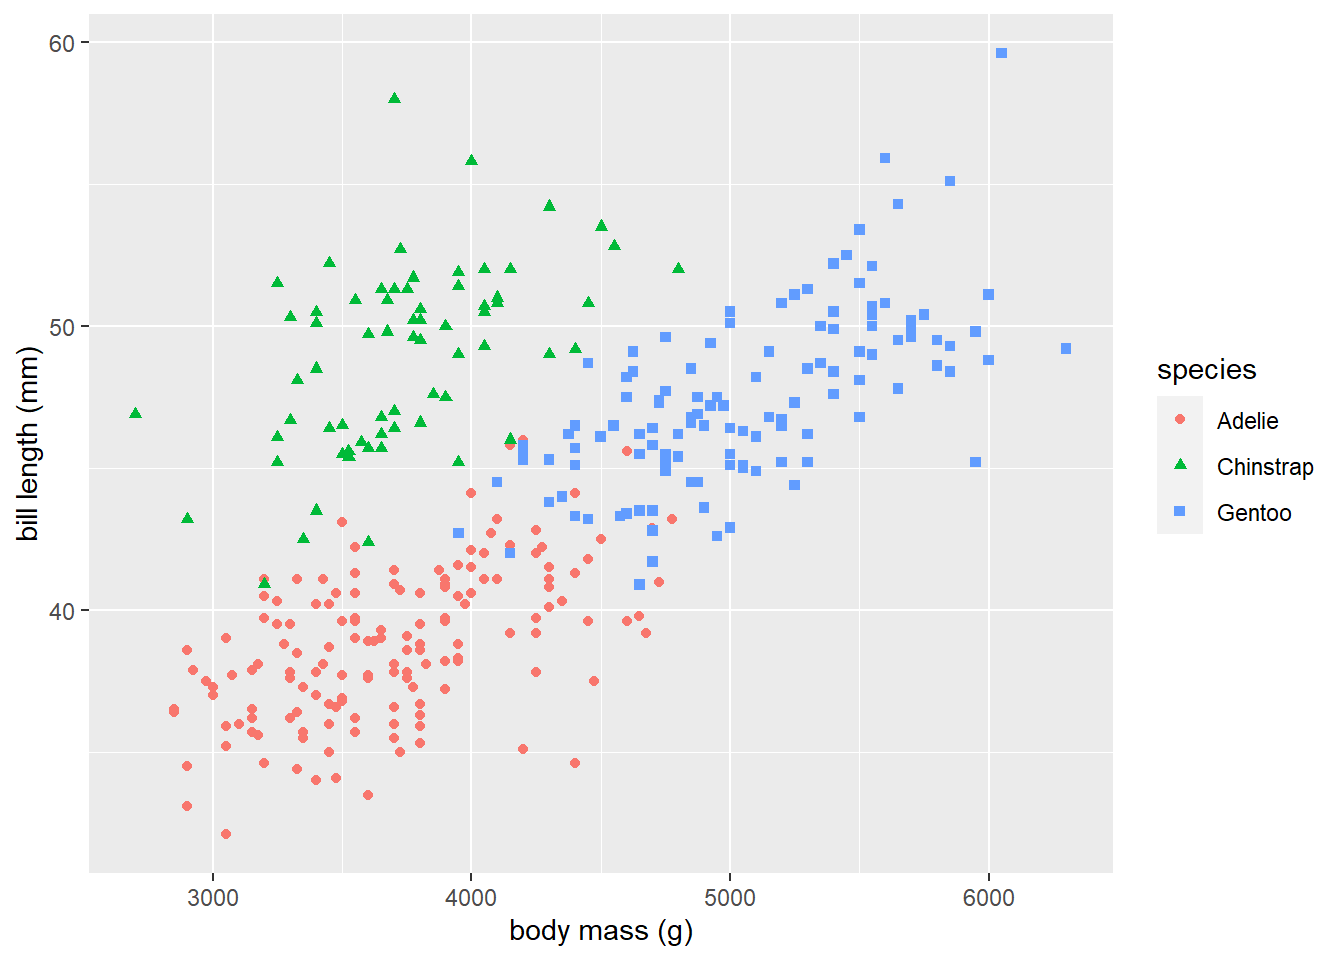
\includegraphics{A-Progessive-Introduction-to-Linear-Models_files/figure-latex/penguins-grouped-scatter-1.pdf}
\caption{\label{fig:penguins-grouped-scatter}A grouped scatter plot of body mass versus bill length that distinguishes penguin species.}
\end{figure}

How do we use a categorical variable in R's \texttt{lm} function? Recall that we should represent our categorical variables as a \texttt{factor} in R. The \texttt{lm} function will automatically convert a \texttt{factor} variable to the correct number of indicator variables when we include the \texttt{factor} variable in our \texttt{formula} argument. R will automatically choose the reference level to be the first level of the \texttt{factor} variable. To add a main effect term for a categorical predictor, we simply add the term to our \texttt{lm} formula. To create an interaction term, we use \texttt{:} between the interacting variables. E.g., if \texttt{c} is a \texttt{factor} variable and \texttt{x} is a \texttt{numeric} variable, we can use the notation \texttt{c:x} in our \texttt{formula} to get all the interactions between \texttt{c} and \texttt{x}.

In our present context, the categorical predictor of interest is \texttt{species}, which has the levels \texttt{Adelie}, \texttt{Chinstrap}, and \texttt{Gentoo}. The \texttt{species} variable is already a \texttt{factor}. Since the variable has 3 levels, it will be transformed into 2 indicator variables by R. The first level of species is \texttt{Adelie}, so R will treat that level as the reference level, and automatically create indicator variables for the levels \texttt{Chinstrap} and \texttt{Gentoo}. (Reminder: to determine the level order of a \texttt{factor} variable \texttt{c}, run the commend \texttt{levels(c)}, or in this case \texttt{levels(penguins\$species)}.)

Let \(D_C\) denote the indicator variable for the \texttt{Chinstrap} level and \(D_G\) denote the indicator variable for the \texttt{Gentoo} level. To fit the parallel lines regression model
\[E(\mathtt{bill\_length\_mm} \mid \mathtt{body\_mass\_g}, \mathtt{species}) = \beta_{0} + \beta_1 \mathtt{body\_mass\_g} + \beta_2 D_C + \beta_3 D_G,\]
we run the code below. The \texttt{coef} function is used to extract the estimated coefficients from our fitted model in \texttt{lmodp}.

\begin{Shaded}
\begin{Highlighting}[]
\CommentTok{\# fit parallel lines model}
\NormalTok{lmodp }\OtherTok{\textless{}{-}} \FunctionTok{lm}\NormalTok{(bill\_length\_mm }\SpecialCharTok{\textasciitilde{}}\NormalTok{ body\_mass\_g }\SpecialCharTok{+}\NormalTok{ species, }\AttributeTok{data =}\NormalTok{ penguins)}
\CommentTok{\# extract coefficients}
\FunctionTok{coef}\NormalTok{(lmodp)}
\DocumentationTok{\#\#      (Intercept)      body\_mass\_g speciesChinstrap }
\DocumentationTok{\#\#     24.919470977      0.003748497      9.920884113 }
\DocumentationTok{\#\#    speciesGentoo }
\DocumentationTok{\#\#      3.557977539}
\end{Highlighting}
\end{Shaded}

Thus, the fitted parallel lines model is
\[
\begin{aligned}
&\hat{E}(\mathtt{bill\_length\_mm} \mid \mathtt{body\_mass\_g}, \mathtt{species}) \\
&= 24.92 + 0.004 \mathtt{body\_mass\_g} + 9.92 D_C + 3.56 D_G.
\end{aligned}
\label{eq:pl-model-penguins}
\]
Note that \texttt{speciesChinstrap} and \texttt{speciesGentoo} are the indicator variables related to the \texttt{Chinstrap} and \texttt{Gentoo} levels of \texttt{species}, respectively, i.e., they represent \(D_C\) and \(D_G\). When an observation has \texttt{species} level \texttt{Adelie}, then Equation \eqref{eq:pl-model-penguins} simplifies to
\[
\begin{aligned}
&\hat{E}(\mathtt{bill\_length\_mm} \mid \mathtt{body\_mass\_g}, \mathtt{species}=\mathtt{Adelie}) \\
&=24.92 + 0.004 \mathtt{body\_mass\_g} + 9.92 \cdot 0 + 3.56 \cdot 0 \\
&= 24.92 + 0.004 \mathtt{body\_mass\_g}.
\end{aligned}
\]
When an observation has \texttt{species} level \texttt{Chinstrap}, then Equation \eqref{eq:pl-model-penguins} simplifies to
\[
\begin{aligned}
&\hat{E}(\mathtt{bill\_length\_mm} \mid \mathtt{body\_mass\_g}, \mathtt{species}=\mathtt{Chinstrap}) \\
&=24.92 + 0.004 \mathtt{body\_mass\_g} + 9.92 \cdot 1 + 3.56 \cdot 0 \\
&= 34.84 + 0.004 \mathtt{body\_mass\_g}.
\end{aligned}
\]
Lastly, when an observation has \texttt{species} level \texttt{Gentoo}, then Equation \eqref{eq:pl-model-penguins} simplifies to
\[
\begin{aligned}
&\hat{E}(\mathtt{bill\_length\_mm} \mid \mathtt{body\_mass\_g}, \mathtt{species}=\mathtt{Gentoo}) \\
&=24.92 + 0.004 \mathtt{body\_mass\_g} + 9.92 \cdot 0 + 3.56 \cdot 1 \\
&= 28.48 + 0.004 \mathtt{body\_mass\_g}.
\end{aligned}
\]
Adding fitted lines for each \texttt{species} level to the scatter plot in Figure \ref{fig:penguins-grouped-scatter} is a bit more difficult than before. One technique is to use \texttt{predict} to get the fitted values of each observation, use the \texttt{transform} function to add those values as a column to the original the data frame, then use \texttt{geom\_line} to connect the fitted values from each group.

We start by adding our fitted values to the \texttt{penguins} data frame. We use the \texttt{predict} function to obtained the fitted values of our fitted model and then use the \texttt{transform} function to add those values as the \texttt{pl\_fitted} variable in the \texttt{penguins} data frame.

\begin{Shaded}
\begin{Highlighting}[]
\NormalTok{penguins }\OtherTok{\textless{}{-}}
\NormalTok{  penguins }\SpecialCharTok{|\textgreater{}}
  \FunctionTok{transform}\NormalTok{(}\AttributeTok{pl\_fitted =} \FunctionTok{predict}\NormalTok{(lmodp))}
\DocumentationTok{\#\# Error in data.frame(structure(list(species = structure(c(1L, 1L, 1L, 1L, : arguments imply differing number of rows: 344, 342}
\end{Highlighting}
\end{Shaded}

We just received a nasty error. What is going on? The original \texttt{penguins} data frame has 344 rows. However, two rows had \texttt{NA} observations such that when we used the \texttt{lm} function to fit our parallel lines model, those observations were removed prior to fitting. The \texttt{predict} function produces fitted values for the observations used in the fitting process, so there are only 342 predicted values. There is a mismatch between the number of rows in \texttt{penguins} and the number of values we attempt to add in the new column \texttt{pl\_fitted}, so we get an error.

To handle this error, we refit our model while setting the \texttt{na.action} argument to \texttt{na.exclude}. As stated Details section of the documentation for the \texttt{lm} function (run \texttt{?lm} in the Console):

\begin{quote}
\(\ldots\) when \texttt{na.exclude} is used the residuals and predictions are padded to the correct length by inserting \texttt{NA}s for cases omitted by \texttt{na.exclude}.
\end{quote}

We refit the parallel lines model below with \texttt{na.action\ =\ na.exclude}, then use the \texttt{predict} function to add the fitted values to the \texttt{penguins} data frame via the \texttt{transform} function.

\begin{Shaded}
\begin{Highlighting}[]
\CommentTok{\# refit parallel lines model with new na.action behavior}
\NormalTok{lmodp }\OtherTok{\textless{}{-}} \FunctionTok{lm}\NormalTok{(bill\_length\_mm }\SpecialCharTok{\textasciitilde{}}\NormalTok{ body\_mass\_g }\SpecialCharTok{+}\NormalTok{ species, }\AttributeTok{data =}\NormalTok{ penguins, }\AttributeTok{na.action =}\NormalTok{ na.exclude)}
\CommentTok{\# add fitted values to penguins data frame}
\NormalTok{penguins }\OtherTok{\textless{}{-}}
\NormalTok{  penguins }\SpecialCharTok{|\textgreater{}}
  \FunctionTok{transform}\NormalTok{(}\AttributeTok{pl\_fitted =} \FunctionTok{predict}\NormalTok{(lmodp))}
\end{Highlighting}
\end{Shaded}

We now use the \texttt{geom\_line} function to add the fitted lines for each \texttt{species} level to our scatter plot. Figure \ref{fig:pl-penguin-fit} displays the results from running the code below. The parallel lines model shown in Figure \ref{fig:pl-penguin-fit} fits the \texttt{penguins} data better than the simple linear regression model shown in Figure \ref{fig:slr-penguin-fit}.

\begin{Shaded}
\begin{Highlighting}[]
\CommentTok{\# create plot}
\CommentTok{\# create scatterplot}
\CommentTok{\# customize labels}
\CommentTok{\# add lines for each level of species}
\FunctionTok{ggplot}\NormalTok{(}\AttributeTok{data =}\NormalTok{ penguins) }\SpecialCharTok{+}
  \FunctionTok{geom\_point}\NormalTok{(}\FunctionTok{aes}\NormalTok{(}\AttributeTok{x =}\NormalTok{ body\_mass\_g, }\AttributeTok{y =}\NormalTok{ bill\_length\_mm,}
                 \AttributeTok{shape =}\NormalTok{ species, }\AttributeTok{color =}\NormalTok{ species)) }\SpecialCharTok{+}
  \FunctionTok{xlab}\NormalTok{(}\StringTok{"body mass (g)"}\NormalTok{) }\SpecialCharTok{+} \FunctionTok{ylab}\NormalTok{(}\StringTok{"bill length (mm)"}\NormalTok{) }\SpecialCharTok{+}
  \FunctionTok{geom\_line}\NormalTok{(}\FunctionTok{aes}\NormalTok{(}\AttributeTok{x =}\NormalTok{ body\_mass\_g, }\AttributeTok{y =}\NormalTok{ pl\_fitted, }\AttributeTok{color =}\NormalTok{ species))}
\end{Highlighting}
\end{Shaded}

\begin{figure}
\centering
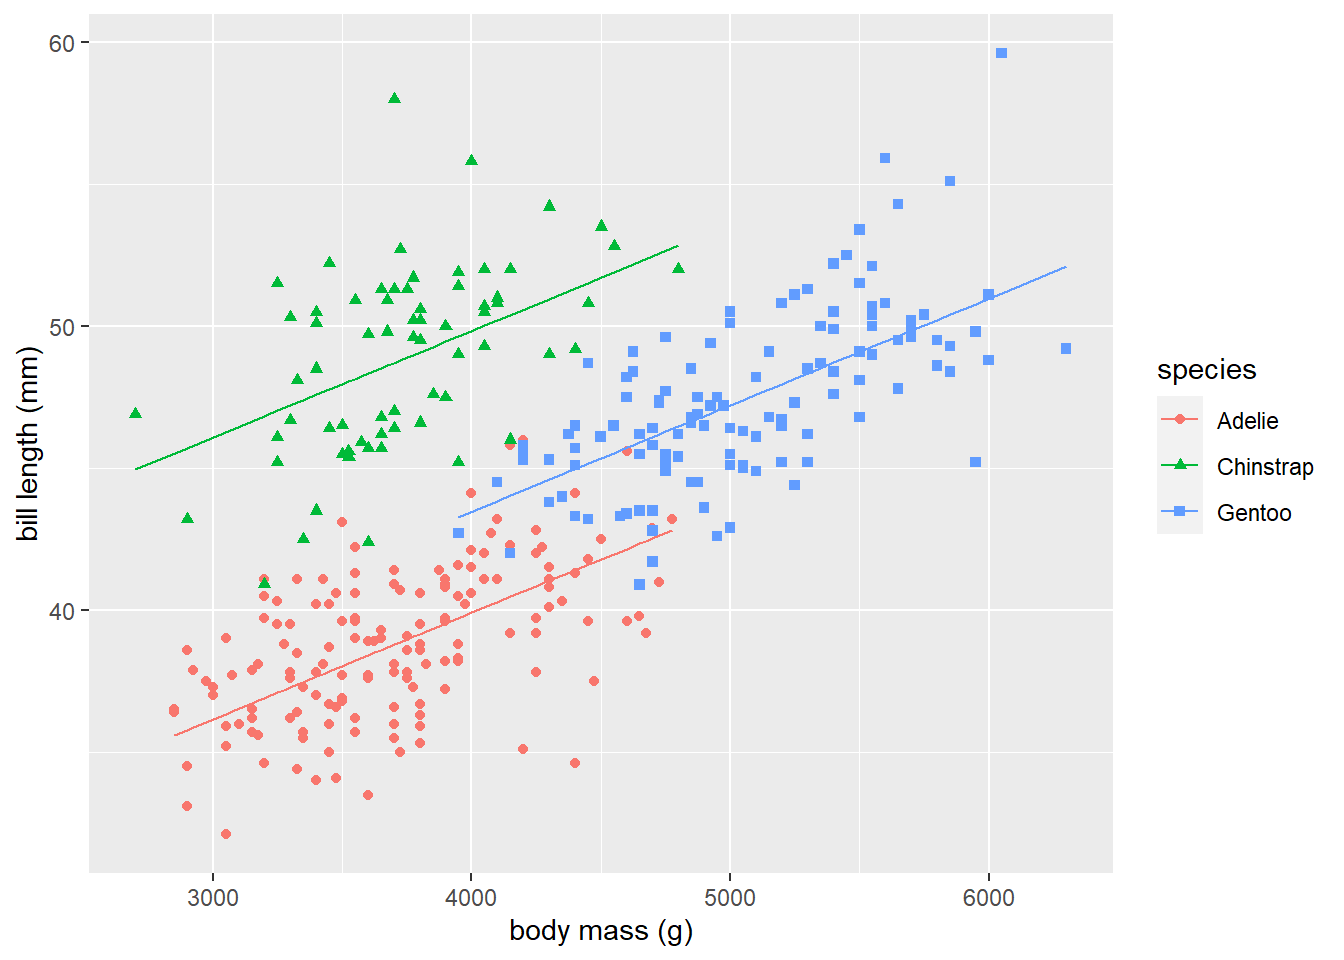
\includegraphics{A-Progessive-Introduction-to-Linear-Models_files/figure-latex/pl-penguin-fit-1.pdf}
\caption{\label{fig:pl-penguin-fit}The fitted lines from the separate lines model for each level of \texttt{species} is added to the grouped scatter plot of \texttt{bill\_length\_mm} versus \texttt{body\_mass\_g}.}
\end{figure}

We now fit a separate lines regression model to the \texttt{penguins} data. Specifically, we fit the model
\[
\begin{aligned}
&E(\mathtt{bill\_length\_mm} \mid \mathtt{body\_mass\_g}, \mathtt{species}) \\
&= \beta_{0} + \beta_1 \mathtt{body\_mass\_g} + \beta_2 D_C + \beta_3 D_G + \beta_4 \mathtt{body\_mass\_g} D_C + \beta_5 \mathtt{body\_mass\_g} D_G ,
\end{aligned}
\]
using the code below, using the \texttt{coef} function to extract the estimated coefficients. The terms with \texttt{:} are interaction variables, e.g., \texttt{body\_mass\_g:speciesChinstrap} is \(\hat{\beta}_4\), the coefficient for the interaction between regressor \(\mathtt{body\_mass\_g} D_C\).

\begin{Shaded}
\begin{Highlighting}[]
\CommentTok{\# fit separate lines model}
\CommentTok{\# na.omit = na.exclude used to change predict behavior}
\NormalTok{lmods }\OtherTok{\textless{}{-}} \FunctionTok{lm}\NormalTok{(bill\_length\_mm }\SpecialCharTok{\textasciitilde{}}\NormalTok{ body\_mass\_g }\SpecialCharTok{+}\NormalTok{ species }\SpecialCharTok{+}\NormalTok{ body\_mass\_g}\SpecialCharTok{:}\NormalTok{species,}
            \AttributeTok{data =}\NormalTok{ penguins, }\AttributeTok{na.action =}\NormalTok{ na.exclude)}
\CommentTok{\# extract estimated coefficients}
\FunctionTok{coef}\NormalTok{(lmods)}
\DocumentationTok{\#\#                  (Intercept)                  body\_mass\_g }
\DocumentationTok{\#\#                26.9941391367                 0.0031878758 }
\DocumentationTok{\#\#             speciesChinstrap                speciesGentoo }
\DocumentationTok{\#\#                 5.1800537287                {-}0.2545906615 }
\DocumentationTok{\#\# body\_mass\_g:speciesChinstrap    body\_mass\_g:speciesGentoo }
\DocumentationTok{\#\#                 0.0012748183                 0.0009029956}
\end{Highlighting}
\end{Shaded}

Thus, the fitted separate lines model is

\[
\begin{aligned}
&\hat{E}(\mathtt{bill\_length\_mm} \mid \mathtt{body\_mass\_g}, \mathtt{species}) \\
&= 26.99 + 0.003 \mathtt{body\_mass\_g} + 5.18 D_C - 0.25 D_G \\
& \quad + 0.001 \mathtt{body\_mass\_g} D_C + 0.0009 \mathtt{body\_mass\_g} D_G. \end{aligned}
\label{eq:sl-model-penguins}
\]

When an observation has \texttt{species} level \texttt{Adelie}, then Equation \eqref{eq:sl-model-penguins} simplifies to

\[
\begin{aligned}
&\hat{E}(\mathtt{bill\_length\_mm} \mid \mathtt{body\_mass\_g}, \mathtt{species}=\mathtt{Adelie}) \\
&=26.99 + 0.003 \mathtt{body\_mass\_g} + 5.18 \cdot 0 - 0.25 \cdot 0\\
&\quad + 0.001 \cdot \mathtt{body\_mass\_g} \cdot 0 + 0.0009 \cdot \mathtt{body\_mass\_g} \cdot 0\\
&= 26.99 + 0.003 \mathtt{body\_mass\_g}.
\end{aligned}
\]

When an observation has \texttt{species} level \texttt{Chinstrap}, then Equation \eqref{eq:sl-model-penguins} simplifies to
\[
\begin{aligned}
&\hat{E}(\mathtt{bill\_length\_mm} \mid \mathtt{body\_mass\_g}, \mathtt{species}=\mathtt{Chinstrap}) \\
&=26.99 + 0.003 \mathtt{body\_mass\_g} + 5.18 \cdot 1 - 0.25 \cdot 0 \\
&\quad + 0.001 \cdot \mathtt{body\_mass\_g} \cdot 1 + 0.0009 \cdot \mathtt{body\_mass\_g} \cdot 0 \\
&= 31.17 + 0.004 \mathtt{body\_mass\_g}.
\end{aligned}
\]
When an observation has \texttt{species} level \texttt{Gentoo}, then Equation \eqref{eq:sl-model-penguins} simplifies to
\[
\begin{aligned}
&\hat{E}(\mathtt{bill\_length\_mm} \mid \mathtt{body\_mass\_g}, \mathtt{species}=\mathtt{Chinstrap}) \\
&=26.99 + 0.003 \mathtt{body\_mass\_g} + 5.18 \cdot 0 - 0.25 \cdot 1 \\
&\quad + 0.001 \cdot \mathtt{body\_mass\_g} \cdot 0 + 0.0009 \cdot \mathtt{body\_mass\_g} \cdot 1 \\
&= 26.74 + 0.004 \mathtt{body\_mass\_g}.
\end{aligned}
\]

We use the code below to display the fitted lines for the separate lines model on the \texttt{penguins} data. Figure \ref{fig:sl-penguin-fit} shows the results. The fitted lines match the observed data behavior reasonably well.

\begin{Shaded}
\begin{Highlighting}[]
\CommentTok{\# add separate lines fitted values to penguins data frame}
\NormalTok{penguins }\OtherTok{\textless{}{-}}
\NormalTok{  penguins }\SpecialCharTok{|\textgreater{}}
  \FunctionTok{transform}\NormalTok{(}\AttributeTok{sl\_fitted =} \FunctionTok{predict}\NormalTok{(lmods))}
\CommentTok{\# use geom\_line to add fitted lines to plot}
\FunctionTok{ggplot}\NormalTok{(}\AttributeTok{data =}\NormalTok{ penguins) }\SpecialCharTok{+}
  \FunctionTok{geom\_point}\NormalTok{(}\FunctionTok{aes}\NormalTok{(}\AttributeTok{x =}\NormalTok{ body\_mass\_g, }\AttributeTok{y =}\NormalTok{ bill\_length\_mm, }\AttributeTok{shape =}\NormalTok{ species, }\AttributeTok{color =}\NormalTok{ species)) }\SpecialCharTok{+}
  \FunctionTok{xlab}\NormalTok{(}\StringTok{"body mass (g)"}\NormalTok{) }\SpecialCharTok{+} \FunctionTok{ylab}\NormalTok{(}\StringTok{"bill length (mm)"}\NormalTok{) }\SpecialCharTok{+}
  \FunctionTok{geom\_line}\NormalTok{(}\FunctionTok{aes}\NormalTok{(}\AttributeTok{x =}\NormalTok{ body\_mass\_g, }\AttributeTok{y =}\NormalTok{ sl\_fitted, }\AttributeTok{col =}\NormalTok{ species))}
\end{Highlighting}
\end{Shaded}

\begin{figure}
\centering
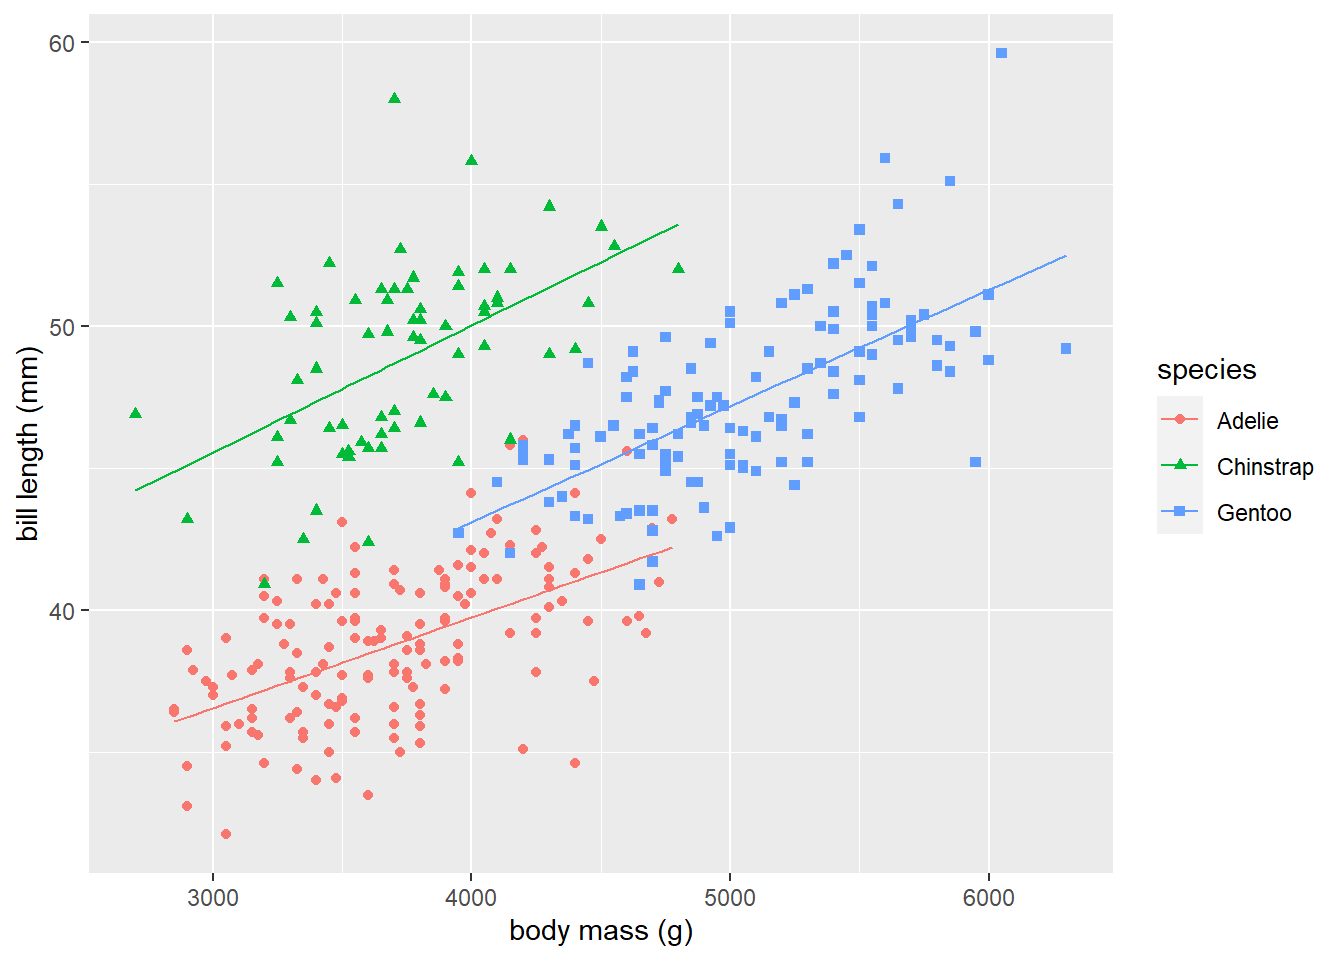
\includegraphics{A-Progessive-Introduction-to-Linear-Models_files/figure-latex/sl-penguin-fit-1.pdf}
\caption{\label{fig:sl-penguin-fit}The fitted model for each level of \texttt{species} is added to the grouped scatter plot of \texttt{bill\_length\_mm} versus \texttt{body\_mass\_g}.}
\end{figure}

Having fit several models for the \texttt{penguins} data, we may be wondering how to evaluate how well the models fit the data. We discuss that in the next section.

\hypertarget{evaluating-model-fit}{%
\section{Evaluating model fit}\label{evaluating-model-fit}}

The most basic statistic measuring the fit of a regression model is the \textbf{coefficient of determination}, which is defined as
\[
R^2 = 1 - \frac{\sum_{i=1}^n (Y_i-\hat{Y}_i)^2}{\sum_{i=1}^n (Y_i-\bar{Y})^2},\label{eq:rsquared}
\]
where \(\bar{Y}\) is the sample mean of the observed response values.

To interpret this statistic, we need to introduce some new ``sum-of-squares'' statistics similar to the RSS.

The \textbf{total sum of squares} (corrected for the mean) is computed as
\[
TSS = \sum_{i=1}^n(Y_i-\bar{Y})^2. \label{eq:tss}
\]
The TSS is the sum of the squared deviations of the response values from the sample mean. However, it has a more insightful interpretation. Consider the \textbf{constant mean model}, which is the model
\[
E(Y)=\beta_0. \label{eq:constant-mean-model}
\]
Using basic calculus, we can show that the OLS estimator of \(\beta_0\) for the model in Equation \eqref{eq:constant-mean-model} is \(\hat{\beta}_0=\bar{Y}\). For the constant mean model, the fitted value of every observation is \(\hat{\beta}_0\), i.e., \(\hat{Y}_i=\hat{\beta}_0\) for \(i=1,2,\ldots,n\). Thus, the RSS of the constant mean model is \(\sum_{i=1}^n(Y_i-\hat{Y}_i)^2=\sum_{i=1}^n(Y_i-\bar{Y})^2\). Thus, \emph{the TSS is the RSS for the constant mean model}.

The \textbf{regression sum-of-squares} or \textbf{model sum-of-squares} is defined as
\[
SS_{reg} = \sum_{i=1}^n(\hat{Y}_i-\bar{Y})^2. \label{eq:ssreg}
\]
Thus, SS\textsubscript{reg} is the sum of the squared deviations between the fitted values of a model and the fitted values of the constant mean model. More helpfully, we have the following equation relating TSS, RSS, and SS\textsubscript{reg}:
\[
TSS = RSS + SS_{reg}.\label{eq:ss-equality}
\]
Thus, \(SS_{reg}=TSS-RSS\). This means that \emph{SS\textsubscript{reg} measures the reduction in RSS when comparing the fitted model to the constant mean model}.

Comparing Equations \eqref{eq:def-rss-slr}, \eqref{eq:rsquared}, \eqref{eq:tss}, and \eqref{eq:ssreg}, we can express \(R^2\) as:
\[
\begin{aligned}
R^2 &= 1-\frac{\sum_{i=1}^n (Y_i-\hat{Y}_i)^2}{\sum_{i=1}^n (Y_i-\bar{Y})^2} \\
&= 1 - \frac{RSS}{TSS} \\
&= \frac{TSS - RSS}{TSS} \\
&= \frac{SS_{reg}}{TSS} \\
&= [\mathrm{cor}(\mathbf{y}, \hat{\mathbf{y}})]^2.
\end{aligned}
\label{eq:rsquared2}
\]
The last expression is the squared sample correlation between the observed and fitted values, and is a helpful way to express the coefficient of determination because it extends to regression models that are not linear.

Looking at Equation \eqref{eq:rsquared2} in particular, we can say that \emph{the coefficient of determination is the proportional reduction in RSS when comparing the fitted model to the constant mean model}.

Some comments about the coefficient of determination:

\begin{itemize}
\tightlist
\item
  \(0\leq R^2 \leq 1\).
\item
  \(R^2=0\) for the constant mean model.
\item
  \(R^2=1\) for a fitted model that perfectly fits the data (the fitted values match the observed response values).
\item
  Generally, larger values of \(R^2\) suggest that the model explains a lot of the variation in the response variable. Smaller \(R^2\) values suggest the fitted model does not explain a lot of the response variation.
\item
  The \texttt{Multiple\ R-squared} value printed by the \texttt{summary} of an \texttt{lm} object is \(R^2\).
\item
  To extract \(R^2\) from a fitted model, we can use the syntax \texttt{summary(lmod)\$r.squared}, where \texttt{lmod} is our fitted model.
\end{itemize}

Figure \ref{fig:rsquared-examples} provides examples of the \(R^2\) value for various fitted simple linear regression models. The closer the points fall to a straight line, the larger \(R^2\) tends to be. However, as shown in the bottom right panel of Figure \ref{fig:rsquared-examples}, a poorly fit model can result in a lower \(R^2\) model even if there is a clear relationship between the points (the points have a perfect quadratic relationship).

\begin{figure}
\centering
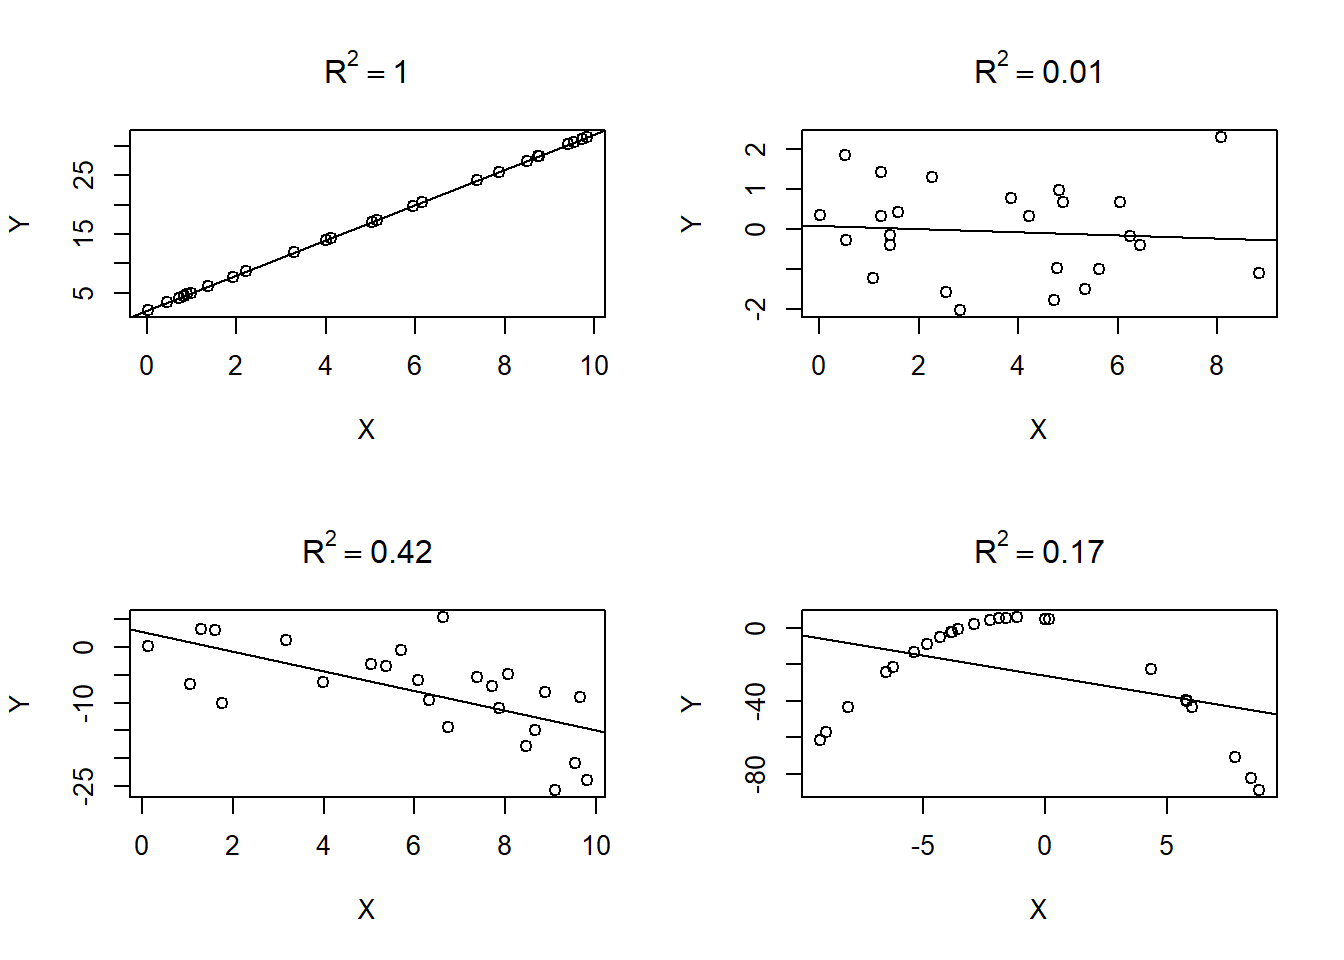
\includegraphics{A-Progessive-Introduction-to-Linear-Models_files/figure-latex/rsquared-examples-1.pdf}
\caption{\label{fig:rsquared-examples}The coefficient of determination values for 4 different data sets.}
\end{figure}

The coefficient of determination for the parallel lines model fit to the \texttt{penguins} data in Section \ref{s:penguins-mlr2} is 0.81, as shown in the R output below. By adding the \texttt{body\_mass\_g} regressor and \texttt{species} predictor to the constant mean model of \texttt{bill\_length\_mm}, we reduced the RSS by 81\%.

\begin{Shaded}
\begin{Highlighting}[]
\FunctionTok{summary}\NormalTok{(lmodp)}\SpecialCharTok{$}\NormalTok{r.squared}
\DocumentationTok{\#\# [1] 0.8079566}
\end{Highlighting}
\end{Shaded}

It may seem sensible to choose between models based on the value of \(R^2\). This is unwise for two reasons:

\begin{enumerate}
\def\labelenumi{\arabic{enumi}.}
\tightlist
\item
  \(R^2\) never decreases as regressors are added to an existing model. Basically, we can increase \(R^2\) by simply adding regressors to our existing model, even if they are non-sensical.
\item
  \(R^2\) doesn't tell us whether a model adequately describes the pattern of the observed data. \(R^2\) is a useful statistic for measuring model fit when there is approximately a linear relationship between the response values and fitted values.
\end{enumerate}

Regarding point 1, consider what happens when we add a regressor of random values to the parallel lines model fit to the \texttt{penguins} data. The code below sets a random number seed so that we can get the same results each time we run the code, creates the regressor \texttt{noisyx} by sampling 344 values randomly drawn from a \(\mathcal{N}(0,1)\) distribution, adds \texttt{noisyx} as a regressor to the parallel lines regression model stored in \texttt{lmodp}, and then extracts the \(R^2\) value. We use the \texttt{update} method to update our existing model. The \texttt{update} function takes an existing model as its first argument and then the \texttt{formula} for the updated model. The syntax \texttt{.\ \textasciitilde{}\ .} means ``keep the same response (on the left) and the same regressors (on the right)''. We can then add or subtract regressors using the typical \texttt{formula} syntax. We use this approach to add the \texttt{noisyx} regressor to the regressors already in \texttt{lmodp}.

\begin{Shaded}
\begin{Highlighting}[]
\FunctionTok{set.seed}\NormalTok{(}\DecValTok{28}\NormalTok{) }\CommentTok{\# for reproducibility}
\CommentTok{\# create regressor of random noise}
\NormalTok{noisyx }\OtherTok{\textless{}{-}} \FunctionTok{rnorm}\NormalTok{(}\DecValTok{344}\NormalTok{)}
\CommentTok{\# add noisyx as regressor to lmodp}
\NormalTok{lmod\_silly }\OtherTok{\textless{}{-}} \FunctionTok{update}\NormalTok{(lmodp, . }\SpecialCharTok{\textasciitilde{}}\NormalTok{ . }\SpecialCharTok{+}\NormalTok{ noisyx)}
\CommentTok{\# extract R\^{}2 from fitted model}
\FunctionTok{summary}\NormalTok{(lmod\_silly)}\SpecialCharTok{$}\NormalTok{r.squared}
\DocumentationTok{\#\# [1] 0.8087789}
\end{Highlighting}
\end{Shaded}

The \(R^2\) value increased from 0.8080 to 0.8088! So clearly, choosing the model with the largest \(R^2\) can be a mistake, as it will tend to favor models with more regressors.

Regarding point 2, \(R^2\) can mislead us into thinking an inappropriate model fits better than it actually does. Anscombe (\protect\hyperlink{ref-anscombe1973graphs}{1973}) provided a canonical data set known as ``Anscombe's quartet'' that illustrates this point. The data set is comprised of 4 different data sets. When a simple linear regression model is fit to each data set, we find that \(\hat{\beta}_0=3\), \(\hat{\beta}_1=0.5\), and that \(R^2=0.67\). However, as we will see, not all models describe the data particularly well!

Anscombe's quartet is available as the \texttt{anscombe} data set in the \textbf{datasets} package. The data set includes 11 observations of
8 variables. The variables are:

\begin{itemize}
\tightlist
\item
  \texttt{x1}, \texttt{x2}, \texttt{x3}, \texttt{x4}: the regressor variable for each individual data set.
\item
  \texttt{y1}, \texttt{y2}, \texttt{y3}, \texttt{y4}: the response variable for each individual data set.
\end{itemize}

We fit the simple linear regression model to the four data sets in the code below, then extract the coefficients and \(R^2\) to verify the information provided above.

\begin{Shaded}
\begin{Highlighting}[]
\CommentTok{\# fit model to first data set}
\NormalTok{lmod\_a1 }\OtherTok{\textless{}{-}} \FunctionTok{lm}\NormalTok{(y1 }\SpecialCharTok{\textasciitilde{}}\NormalTok{ x1, }\AttributeTok{data =}\NormalTok{ anscombe)}
\CommentTok{\# extract coefficients from fitted model}
\FunctionTok{coef}\NormalTok{(lmod\_a1)}
\DocumentationTok{\#\# (Intercept)          x1 }
\DocumentationTok{\#\#   3.0000909   0.5000909}
\CommentTok{\# extract R\^{}2 from fitted model}
\FunctionTok{summary}\NormalTok{(lmod\_a1)}\SpecialCharTok{$}\NormalTok{r.squared}
\DocumentationTok{\#\# [1] 0.6665425}
\CommentTok{\# fit model to second data set}
\NormalTok{lmod\_a2 }\OtherTok{\textless{}{-}} \FunctionTok{lm}\NormalTok{(y2 }\SpecialCharTok{\textasciitilde{}}\NormalTok{ x2, }\AttributeTok{data =}\NormalTok{ anscombe)}
\FunctionTok{coef}\NormalTok{(lmod\_a2)}
\DocumentationTok{\#\# (Intercept)          x2 }
\DocumentationTok{\#\#    3.000909    0.500000}
\FunctionTok{summary}\NormalTok{(lmod\_a2)}\SpecialCharTok{$}\NormalTok{r.squared}
\DocumentationTok{\#\# [1] 0.666242}
\CommentTok{\# fit model to third data set}
\NormalTok{lmod\_a3 }\OtherTok{\textless{}{-}} \FunctionTok{lm}\NormalTok{(y3 }\SpecialCharTok{\textasciitilde{}}\NormalTok{ x3, }\AttributeTok{data =}\NormalTok{ anscombe)}
\FunctionTok{coef}\NormalTok{(lmod\_a3)}
\DocumentationTok{\#\# (Intercept)          x3 }
\DocumentationTok{\#\#   3.0024545   0.4997273}
\FunctionTok{summary}\NormalTok{(lmod\_a3)}\SpecialCharTok{$}\NormalTok{r.squared}
\DocumentationTok{\#\# [1] 0.666324}
\CommentTok{\# fit model to fourth data set}
\NormalTok{lmod\_a4 }\OtherTok{\textless{}{-}} \FunctionTok{lm}\NormalTok{(y4 }\SpecialCharTok{\textasciitilde{}}\NormalTok{ x4, }\AttributeTok{data =}\NormalTok{ anscombe)}
\FunctionTok{coef}\NormalTok{(lmod\_a4)}
\DocumentationTok{\#\# (Intercept)          x4 }
\DocumentationTok{\#\#   3.0017273   0.4999091}
\FunctionTok{summary}\NormalTok{(lmod\_a4)}\SpecialCharTok{$}\NormalTok{r.squared}
\DocumentationTok{\#\# [1] 0.6667073}
\end{Highlighting}
\end{Shaded}

Figure \ref{fig:anscombe-plots} provides a scatter plot each data set and overlays their fitted models.

\begin{figure}
\centering
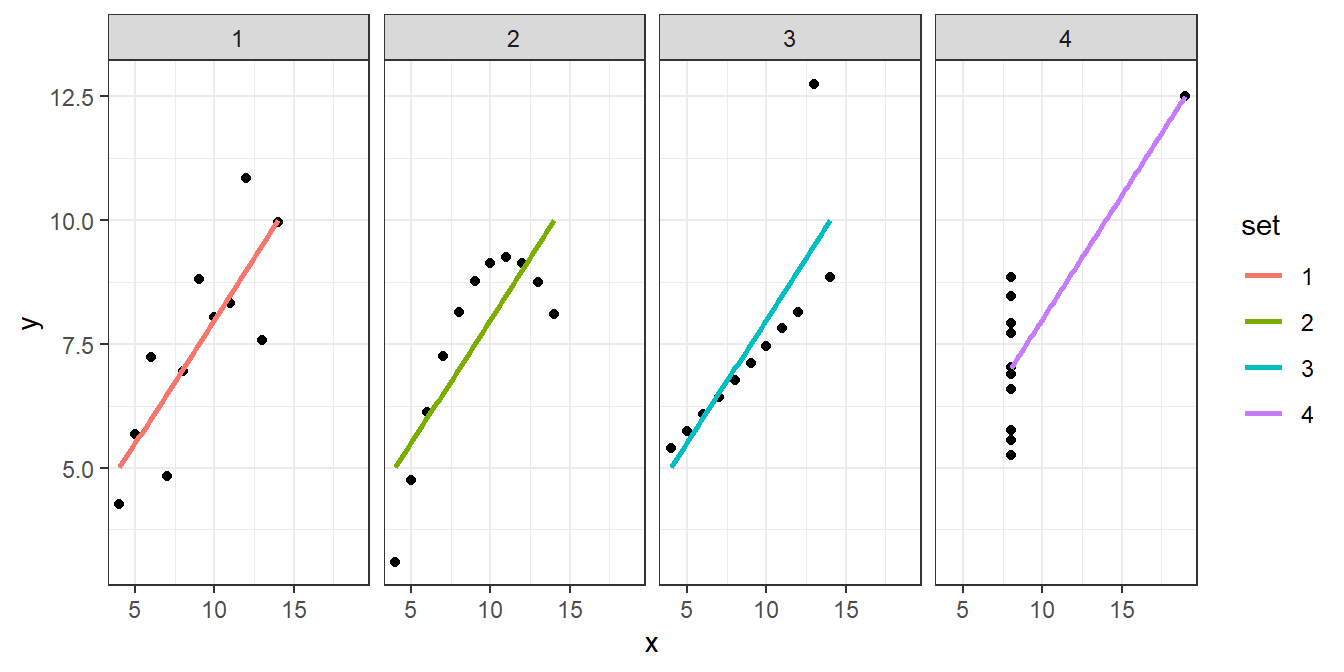
\includegraphics{A-Progessive-Introduction-to-Linear-Models_files/figure-latex/anscombe-plots-1.pdf}
\caption{\label{fig:anscombe-plots}Scatter plots of the four Anscombe data sets along with their line of best fit.}
\end{figure}

While the fitted model and \(R^2\) value is essentially the same for each model, the fitted model is only appropriate for data set 1. The fitted model for the second data set fails to model the curve of the data. The third fitted model doesn't handle the outlier in the data. Lastly, the fourth data set has a single point on the far right side driving the model fit, so the fitted model is highly questionable.

To address the problem with \(R^2\) that it cannot decrease as regressors are added to a model, Ezekiel (\protect\hyperlink{ref-ezekiel1930methods}{1930}) proposed the adjusted R-squared statistic for measuring model fit. The adjusted \(R^2\) statistic is defined as
\[
R^2_a=1-(1-R^2)\frac{n-1}{n-p}=1-\frac{RSS/(n-p)}{TSS/(n-1)}.
\]
Practically speaking, \(R^2_a\) will only increase when a regressors substantively improves the fit of the model to the observed data. We favor models with larger values of \(R^2_a\). To extract the adjusted R-squared from a fitted model, we can use the syntax \texttt{summary(lmod)\$adj.R.squared}, where \texttt{lmod} is the fitted model.

Using the code below, we extract the \(R^2_a\) for the 4 models we previously fit to the \texttt{penguins} data. Specifically, we extract \(R_a^2\) for the simple linear regression model fit in Section \ref{s:penguins-slr}, the multiple linear regression model in Section \ref{s:penguins-mlr}, and the parallel and separate lines models fit in Section \ref{s:penguins-mlr2}.

\begin{Shaded}
\begin{Highlighting}[]
\CommentTok{\# simple linear regression model}
\FunctionTok{summary}\NormalTok{(lmod)}\SpecialCharTok{$}\NormalTok{adj.r.squared}
\DocumentationTok{\#\# [1] 0.3522562}
\CommentTok{\# multiple linear regression model}
\FunctionTok{summary}\NormalTok{(mlmod)}\SpecialCharTok{$}\NormalTok{adj.r.squared}
\DocumentationTok{\#\# [1] 0.4295084}
\CommentTok{\# parallel lines model}
\FunctionTok{summary}\NormalTok{(lmodp)}\SpecialCharTok{$}\NormalTok{adj.r.squared}
\DocumentationTok{\#\# [1] 0.8062521}
\CommentTok{\# separate lines model}
\FunctionTok{summary}\NormalTok{(lmods)}\SpecialCharTok{$}\NormalTok{adj.r.squared}
\DocumentationTok{\#\# [1] 0.8069556}
\end{Highlighting}
\end{Shaded}

With an \(R_a^2\) of 0.8070, the separate lines regression model appears to be slightly favored over the other 3 models fit to the \texttt{penguins} data. To confirm that this statistic is meaningful (i.e., that the model provides a reasonable fit to the data), we use the code below to create a scatter plot of the response versus fitted values shown in Figure \ref{fig:y-vs-yhat-penguins}. The points in Figure \ref{fig:y-vs-yhat-penguins} follow a linear pattern, so the separate lines model seems to be a reasonable model for the \texttt{penguins} data.

\begin{Shaded}
\begin{Highlighting}[]
\FunctionTok{plot}\NormalTok{(penguins}\SpecialCharTok{$}\NormalTok{bill\_length\_mm }\SpecialCharTok{\textasciitilde{}} \FunctionTok{fitted}\NormalTok{(lmods),}
     \AttributeTok{xlab =} \StringTok{"fitted values"}\NormalTok{, }\AttributeTok{ylab =} \StringTok{"bill length (mm)"}\NormalTok{)}
\end{Highlighting}
\end{Shaded}

\begin{figure}
\centering
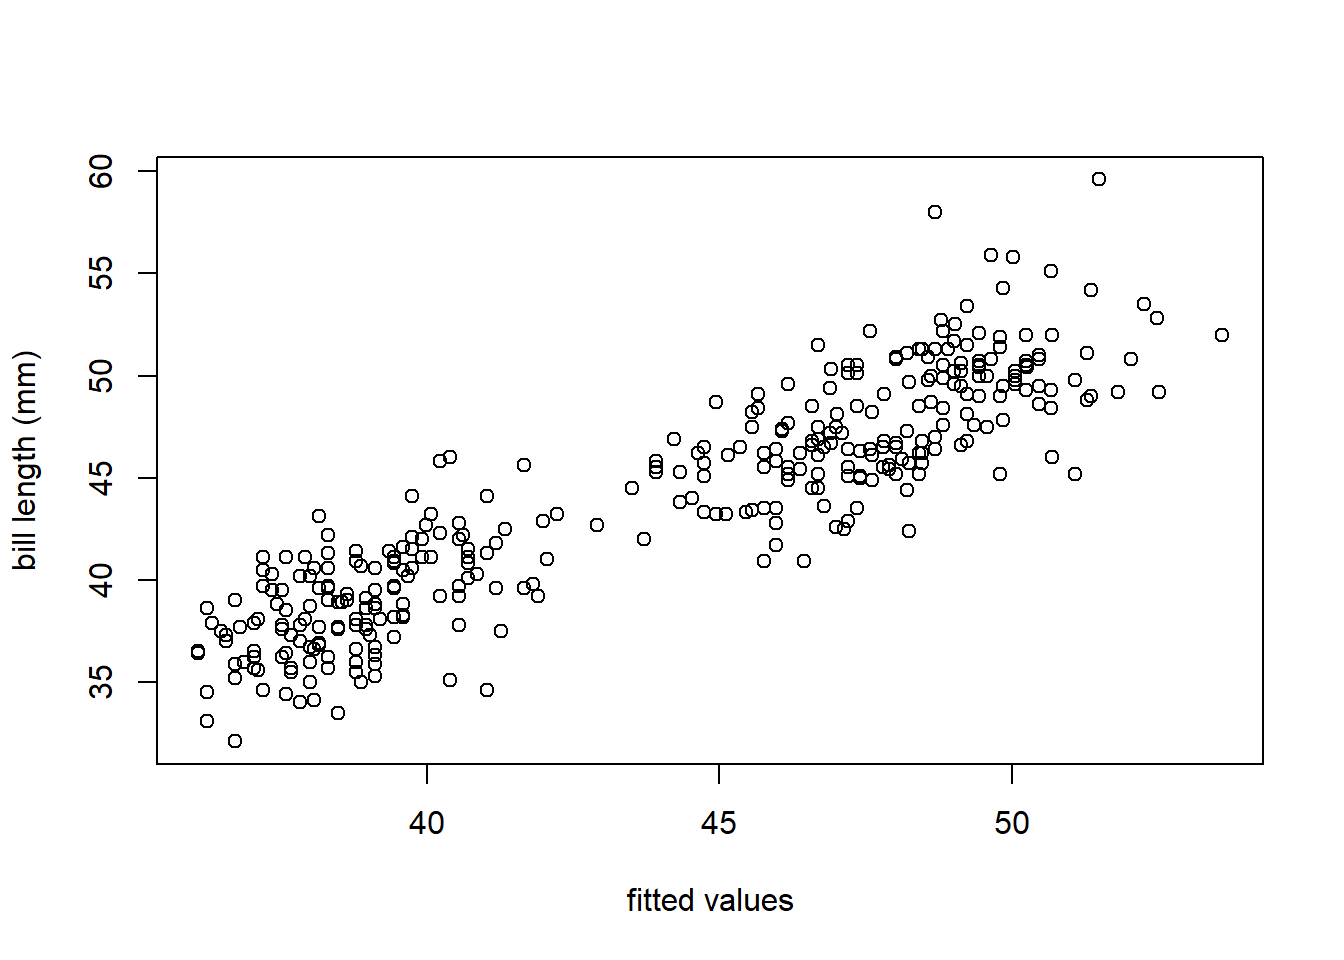
\includegraphics{A-Progessive-Introduction-to-Linear-Models_files/figure-latex/y-vs-yhat-penguins-1.pdf}
\caption{\label{fig:y-vs-yhat-penguins}A scatter plot of the observed bill length versus the fitted values of the separate lines model for the \texttt{penguins} data.}
\end{figure}

\hypertarget{summary}{%
\section{Summary}\label{summary}}

In this chapter, we learned:

\begin{itemize}
\tightlist
\item
  What a linear model is.
\item
  What various objects are, such as coefficients, residuals, fitted values, etc.
\item
  How to estimate the coefficients of a linear model using ordinary least squares estimation.
\item
  How to fit a linear model using R.
\item
  How to include a categorical predictor in a linear model.
\item
  How to evaluate the fit of a model.
\end{itemize}

\hypertarget{ss:term-summary}{%
\subsection{Summary of terms}\label{ss:term-summary}}

We have introduced many terms to define a linear model. It can be difficult to keep track of their notation, their purpose, whether they are observable, and whether they are treated as random variables or vectors. We discuss various terms below, and then summarize the discussion in Table \ref{tab:term-df}.

We've already talked about observing the response variable and the predictor/regressor variables. So these objects are observable. However, we have no way to measure the regression coefficients or the error. These are not observable. One way to distinguish observable versus non-observable variables is that observable variables are denoted using Phoenician letters (e.g., \(X\) and \(Y\)) while non-observable variables are denoted using Greek letters (e.g., \(\beta_j\), \(\epsilon\), \(\sigma^2\)).

We treat the response variable as a random variable. Perhaps surprisingly, we treat the predictor and regressor variables as fixed, non-random variables. The regression coefficients are treated as fixed, non-random but unknown values. This is standard for parameters in a statistical model. The errors are also treated as random variables. In fact, since both the regressor variables and the regression coefficients are non-random, the only way for the responses in Equation \eqref{eq:lmSystem} to be random variables is for the errors to be random.

\begin{table}

\caption{\label{tab:term-df}An overview of terms used to define a linear model.}
\centering
\begin{tabular}[t]{l>{\raggedright\arraybackslash}p{2in}ll}
\toprule
Term & Description & Observable? & Random?\\
\midrule
$Y$ & response variable & Yes & Yes\\
$Y_i$ & response value for the $i$th observation & Yes & Yes\\
$\mathbf{y}$ & the $n\times 1$ column vector of response values & Yes & Yes\\
$X$ & regressor variable & Yes & No\\
$X_j$ & the $j$th regressor variable & Yes & No\\
\addlinespace
$x_{i,j}$ & the value of the $j$th regressor variable for the $i$th observation & Yes & No\\
$\mathbf{X}$ & the $n\times p$ matrix of regressor values & Yes & No\\
$\mathbf{x}_i$ & the $p\times 1$ vector of regressor values for the $i$th observation & Yes & No\\
$\beta_j$ & the coefficient associated with the $j$th regressor variable & No & No\\
$\boldsymbol{\beta}$ & the $p\times 1$ column vector of regression coefficients & No & No\\
\addlinespace
$\epsilon$ & the model error & No & Yes\\
$\epsilon_i$ & the error for the $i$th observation & No & Yes\\
$\boldsymbol{\epsilon}$ & the $n\times 1$ column vector of errors & No & Yes\\
\bottomrule
\end{tabular}
\end{table}

\hypertarget{summary-of-functions}{%
\subsection{Summary of functions}\label{summary-of-functions}}

We have used many functions in this Chapter. We summarize some of the most important ones in Table \ref{tab:function-df}.

\begin{table}

\caption{\label{tab:function-df}An overview of important functions discussed in this chapter.}
\centering
\begin{tabular}[t]{l>{\raggedright\arraybackslash}p{3in}}
\toprule
Function & Purpose\\
\midrule
`lm` & Fits a linear model based on a provided `formula`\\
`summary` & Provides summary information about the fitted model\\
`coef` & Extracts the vector of estimated regression coefficients from the fitted model\\
`residuals` & Extracts the vector of residuals from the fitted model\\
`fitted` & Extracts the vector of fitted values from the fitted model\\
\addlinespace
`predict` & Computes the fitted values (or arbitrary predictions) based on a fitted model\\
`deviance` & Extracts the RSS of a fitted model\\
`sigma` & Extracts $\hat{\sigma}$ from the fitted model\\
`update` & Updates a fitted model to remove or add regressors\\
\bottomrule
\end{tabular}
\end{table}

\hypertarget{going-deeper}{%
\section{Going Deeper}\label{going-deeper}}

\hypertarget{degrees-of-freedom}{%
\subsection{Degrees of freedom}\label{degrees-of-freedom}}

The degrees of freedom of a statistics refers to the number of independent pieces of information that go into its calculation.

Consider the sample mean
\[\bar{x}=\sum_{i=1}^n x_i.\]

The calculation uses \(n\) pieces of information to compute, but the statistic only has \(n-1\) degrees of freedom. Once we know the sample mean, only \(n-1\) values are independent, while the last is constrained to be a certain value.

Let's say \(n=3\) and \(\bar{x} = 10\). Then \(x_1\) and \(x_2\) can be any numbers, but the last value MUST equal \(30 - x_1 - x_2\) so that \(x_1 + x_2 + x_3 = 30\) (otherwise the sample mean won't equal 10). To be more specific, if \(x_1 = 5\) and \(x_2 = 25\), then \(x_3\) must be 0, otherwise the sample mean won't be 10.

\hypertarget{slr-derivation}{%
\subsection{Derivation of the OLS estimators of the simple linear regression model coefficients}\label{slr-derivation}}

Assume a simple linear regression model with \(n\) observations. The residual sum of squares for the simple linear regression model is
\[
RSS(\hat\beta_0, \hat\beta_1) = \sum_{i=1}^n(Y_i - \hat\beta_0 - \hat\beta_1x_i)^2.
\]

\textbf{OLS estimator of \(\beta_0\)}

First, we take the partial derivative of the RSS with respect to \(\hat\beta_0\) and simplify:
\[
\begin{aligned}
\frac{\partial RSS(\hat\beta_0, \hat\beta_1)}{\partial \hat\beta_0} &= \frac{\partial}{\partial \hat\beta_0}\sum_{i=1}^n(Y_i - \hat\beta_0 - \hat\beta_1x_i)^2 & \tiny\text{ (substituting the formula for the RSS)} \\
&= \sum_{i=1}^n \frac{\partial}{\partial \hat\beta_0}(Y_i - \hat\beta_0 - \hat\beta_1x_i)^2  & \tiny\text{ (by the linearity property of derivatives)} \\
&= -2\sum_{i=1}^n(Y_i - \hat\beta_0 - \hat\beta_1x_i). & \tiny\text{ (chain rule, factoring out -2)}
\end{aligned}
\]

Next, we set the partial derivative equal to zero and rearrange the terms to solve for \(\hat{\beta}_0\):
\[
\begin{aligned}
0 &= \frac{\partial RSS(\hat\beta_0, \hat\beta_1)}{\partial \hat\beta_0}  &  \\
0 &= -2\sum_{i=1}^n(Y_i - \hat\beta_0 - \hat\beta_1x_i) & \tiny\text{ (substitute partial deriviative)}\\
0 &= \sum_{i=1}^n(Y_i - \hat\beta_0 - \hat\beta_1x_i) & \tiny\text{ (divide both sides by -2)} \\
0 &= \sum_{i=1}^n Y_i - \sum_{i=1}^n\hat\beta_0 - \sum_{i=1}^n\hat\beta_1x_i &\tiny\text{ (by linearity of sum)} \\
0 &= \sum_{i=1}^n Y_i - n\hat\beta_0 - \sum_{i=1}^n\hat\beta_1x_i & \tiny(\text{sum }\hat\beta_0\ n\text{ times equals }n\hat\beta_0) \\
n\hat\beta_0 &= \sum_{i=1}^n Y_i-\hat{\beta}_1\sum_{i=1}^nx_i. &\tiny\text{ (algebra rearrange, factor }\hat{\beta}_1\text{)} \\
\end{aligned}
\]

Finally, we divide both sides by \(n\) to get the OLS estimator for \(\hat\beta_0\) in terms of \(\hat\beta_1\):
\[
\hat\beta_0 = \bar Y-\hat\beta_1\bar x
\]

\textbf{OLS Estimator of \(\beta_1\)}

Similar to the previous derivation, we differentiate the RSS with respect to the parameter estimate of interest, set the derivative equal to zero, and solve for the parameter.

We start by taking the partial derivative of the RSS with respect to \(\hat{\beta}_1\) and simplify.
\[
\begin{aligned}
\frac{\partial RSS(\hat\beta_0, \hat\beta_1)}{\partial \hat\beta_1} &= \frac{\partial}{\partial \hat\beta_1}\sum_{i=1}^n (Y_i - \hat\beta_0 - \hat\beta_1x_i)^2 & \tiny\text{ (substitute formula for RSS)} \\
&= \sum_{i=1}^n \frac{\partial}{\partial \hat\beta_1}(Y_i - \hat\beta_0 - \hat\beta_1x_i)^2 & \tiny\text{ (linearity property of derivatives)} \\
&= -2\sum_{i=1}^n(Y_i-\hat\beta_0-\hat\beta_1x_i)x_i & \tiny\text{ (chain rule, factor out -2)}
\end{aligned}
\]

We now set this derivative equal to 0 and rearrange the terms to solve for \(\hat{\beta}_1\):
\[
\begin{aligned}
0 &= \frac{\partial RSS(\hat\beta_0, \hat\beta_1)}{\partial \hat\beta_1} & \\
0 &= -2\sum_{i=1}^n(Y_i-\hat\beta_0-\hat\beta_1x_i)x_i &\tiny\text{(substitute partial derivative})\\
0 &= \sum_{i=1}^n(Y_i-(\bar Y -\hat \beta_1\bar x)-\hat\beta_1x_i)x_i &\tiny\text{(substitute OLS estimator of }\hat\beta_0, \text{ divide both sides by -2}) \\
0 &= \sum_{i=1}^n x_iY_i -\sum_{i=1}^n x_i\bar Y+\hat\beta_1\bar x\sum_{i=1}^n x_i-\hat\beta_1\sum_{i=1}^n x_i^2. &\tiny\text{(expand sum, use linearity of sum)} \\
\end{aligned}
\]

Continuing from the previous line, we move the terms involving \(\hat{\beta}_1\) to the other side of the equality to get
\[
\begin{aligned}
\hat\beta_1\sum_{i=1}^n x_i^2-\hat\beta_1\bar x\sum_{i=1}^n x_i &=\sum_{i=1}^n x_iY_i -\sum_{i=1}^n x_i\bar Y & \tiny\text{(move estimator to other side)}\\
\hat\beta_1\sum_{i=1}^n x_i^2-\hat\beta_1\frac{1}{n}\sum_{i=1}^n  x_i\sum_{i=1}^n x_i&=\sum_{i=1}^n x_iY_i -\sum_{i=1}^n x_i\frac{1}{n}\sum_{i=1}^n  Y_i  &\tiny\text{(rewrite using definition of sample means)} \\
\hat\beta_1\sum_{i=1}^n x_i^2-\hat\beta_1\frac{1}{n}\left(\sum_{i=1}^n  x_i\right)^2 &=\sum_{i=1}^n x_iY_i -\frac{1}{n}\sum_{i=1}^n x_i\sum_{i=1}^n  Y_i  & \tiny\text{(reorder and simplify)} \\
\hat\beta_1\left(\sum_{i=1}^n x_i^2-\frac{1}{n}\left(\sum_{i=1}^n  x_i\right)^2\right)&=\sum_{i=1}^n x_iY_i -\frac{1}{n}\sum_{i=1}^n x_i\sum_{i=1}^n  Y_i, & \tiny\text{(factoring)}\\
\end{aligned}
\]
which allows us to obtain
\[
\hat\beta_1=\frac{\sum_{i=1}^n x_iY_i -\frac{1}{n}\sum_{i=1}^n x_i\sum_{i=1}^n  Y_i}{\sum_{i=1}^n x_i^2-\frac{1}{n}\left(\sum_{i=1}^n  x_i\right)^2}.
\]

Thus, we have the OLS estimators of the simple linear regression coefficients are
\[
\begin{aligned}
\hat\beta_0 &= \bar Y-\hat\beta_1\bar x, \\
\hat\beta_1 & =\frac{\sum_{i=1}^n x_iY_i -\frac{1}{n}\sum_{i=1}^n x_i\sum_{i=1}^n Y_i}{\sum_{i=1}^n x_i^2-\frac{1}{n}\left(\sum_{i=1}^n x_i\right)^2}.
\end{aligned}
\]

\hypertarget{unbiasedness-of-ols-estimators}{%
\subsection{Unbiasedness of OLS estimators}\label{unbiasedness-of-ols-estimators}}

We now show that the OLS estimators we derived in Section \ref{slr-derivation} are unbiased. An estimator is unbiased if the expected value is equal to the parameter it is estimating.

The OLS estimator assumes we know the value of the regressor variables for all observations. Thus, we must condition our expectation on knowing the regressor matrix \(\mathbf{X}\). Thus, we want to show that
\[
E(\hat{\beta}_0\mid \mathbf{X})=\beta_0,
\]
where ``\(\mid \mathbf{X}\)'' is convenient notation to indicate that we are conditioning our expectation on knowing the regressor values for every observation.

In Section \ref{s-slr-estimation}, we noted that we assume \(E(\epsilon \mid X)=0\), which is true for every error in our model, i.e.~\(E(\epsilon_i \mid X = x_i) = 0\) for \(i=1,2,\ldots,n\). Thus,

\[
\begin{aligned}
E(Y_i\mid X=x_i) &= E(\beta_0 + \beta_1 x_i +\epsilon_i\mid X = x_i) & \tiny\text{(substiute definition of $Y_i$)} \\
&= E(\beta_0\mid X=x_i) + E(\beta_1 x_i \mid X = X_i) +E(\epsilon_i | X=x_i) & \tiny\text{(linearity property of expectation)} \\
&= \beta_0+\beta_1x_i +E(\epsilon_i | X=x_i) & \tiny\text{(the $\beta$s and $x_i$ are non-random values)} \\
&= \beta_0+\beta_1x_i + 0 & \tiny\text{(assumption about errors)} \\
&= \beta_0+\beta_1x_i. &
\end{aligned}
\]

In the derivations below, every sum is over all values of \(i\), i.e., \(\sum \equiv \sum_{i=1}^n\). We drop the index for simplicity.

Next, we note:
\[
\begin{aligned}
E\left(\sum x_iY_i \biggm| \mathbf{X} \right) &= \sum E(x_iY_i \mid \mathbf{X}) &\tiny\text{ (by the linearity of the expectation operator)}\\
&=\sum x_iE(Y_i\mid \mathbf{X})&\tiny(x_i\text{ is a fixed value, so it can be brought out})\\
&=\sum x_i(\beta_0+\beta_1 x_i)&\tiny\text{(substitute expected value of }Y_i)\\
&=\sum x_i\beta_0+\sum x_i\beta_1 x_i&\tiny\text{(distribute sum)}\\
&=\beta_0\sum x_i+\beta_1\sum x_i^2.&\tiny\text{(factor out constants)}
\end{aligned}
\]

Also,
\[
\begin{aligned}
E(\bar Y\mid \mathbf{X})
&= E\left(\frac{1}{n}\sum Y_i\Biggm|\mathbf{X} \right)&\tiny\text{(definition of sample mean)}\\
&= \frac{1}{n}E\left(\sum Y_i \Bigm| \mathbf{X}\right)&\tiny\text{(factor out constant)}\\
&= \frac{1}{n}\sum E\left(Y_i \mid \mathbf{X}\right)&\tiny\text{(linearity of expectation)}\\
&= \frac{1}{n}\sum(\beta_0+\beta_1 x_i)&\tiny\text{(substitute expected value of }Y_i)\\
&= \frac{1}{n}\left(\sum\beta_0+\sum\beta_1 x_i\right)&\tiny\text{(distribute sum)}\\
&= \frac{1}{n}\left(n\beta_0+\beta_1\sum x_i\right)&\tiny\text{(simplify, factor out constant)}\\
&= \beta_0+\beta_1\bar x. &\tiny\text{(simplify)}
\end{aligned}
\]

To simplify our derivation below, define
\[
SSX = \sum x_i^2-\frac{1}{n}\left(\sum  x_i\right)^2.
\]
Thus,

\[
\begin{aligned}
&E(\hat\beta_1 \mid \mathbf{X}) &\\
&= E\left(\frac{\sum x_iY_i -\frac{1}{n}\sum x_i\sum Y_i}{\sum x_i^2-\frac{1}{n}\left(\sum  x_i\right)^2} \Biggm| \mathbf{X} \right) &\tiny\text{(substitute OLS estimator)} \\
&= \frac{1}{SSX}E\left(\sum x_iY_i-\frac{1}{n}\sum x_i\sum Y_i \biggm| \mathbf{X}\right)&\tiny\text{(factor out constant denominator, substitute }SSX\text{)} \\
&= \frac{1}{SSX}\left[E\left(\sum x_iY_i\Bigm|\mathbf{X}\right)-E\left(\frac{1}{n}\sum x_i\sum Y_i\biggm|\mathbf{X}\right)\right]&\tiny\text{(linearity of expectation)}\\
&= \frac{1}{SSX}\left[E\left(\sum x_iY_i\Bigm|\mathbf{X}\right)-\left(\sum x_i\right)E\left(\bar Y\mid \mathbf{X}\right)\right]&\tiny\text{(factor out constant }\sum x_i\text{, use definition of}\bar{Y})\\
&= \frac{1}{SSX}\left[\left(\beta_0\sum x_i + \beta_1\sum x_i^2\right)-\left(\sum x_i\right)(\beta_0+\beta_1\bar x)\right]&\tiny\text{(substitute previous derivations
)}\\
&= \frac{1}{SSX}\left[\beta_0\sum x_i+\beta_1\sum x_i^2-\beta_0\sum x_i-\beta_1\bar x\sum x_i\right]&\tiny\text{(expand product and reorder)} \\
&= \frac{1}{SSX}\left[\beta_1\sum x_i^2-\beta_1\bar x\sum x_i\right]&\tiny\text{(cancel terms)}\\
&= \frac{1}{SSX}\left[\beta_1\sum x_i^2-\beta_1\frac{1}{n}\sum x_i\sum x_i\right]&\tiny\text{(using definition of sample mean)}\\
&= \frac{1}{SSX}\beta_1\left[\sum x_i^2-\frac{1}{n}\left(\sum x_i\right)^2\right]&\tiny\text{(factor out }\beta_1\text{, simplify})\\
&= \frac{1}{SSX}\beta_1[SSX]&\tiny\text{(substitute }SSX\text{)} \\
&=\beta_1. &\tiny\text{(simplify)}
\end{aligned}
\]

Therefore, \(\hat\beta_1\) is an unbiased estimator of \(\beta_1\).

Next, we show that \(\hat\beta_0\) is unbiased:
\[
\begin{aligned}
E(\hat\beta_0\mid \mathbf{X}) &= E(\bar Y - \hat{\beta}_1\bar x\mid \mathbf{X}) &\tiny\text{(OLS estimator of }\beta_0) \\
&= E(\bar{Y}\mid \mathbf{X}) - E(\hat\beta_1\bar{x}\mid \mathbf{X}) &\tiny\text{(linearity of expectation})\\
&= E(\bar{Y}\mid \mathbf{X}) - \bar{x}E(\hat\beta_1\mid \mathbf{X}) &\tiny\text{(factor out constant})\\
&= \beta_0 +\beta_1\bar x-\bar x\beta_1 &\tiny\text{(substitute previous derivations})\\
&= \beta_0. &\tiny\text{(cancel terms})\\
\end{aligned}
\]

Therefore, \(\hat\beta_0\) is an unbiased estimator of \(\beta_0\).

\hypertarget{manual-calculation-penguins-simple-linear-regression-example}{%
\subsection{Manual calculation Penguins simple linear regression example}\label{manual-calculation-penguins-simple-linear-regression-example}}

In this section, we manually produce (i.e., without the \texttt{lm} function) the \texttt{penguins} simple linear regression example in Section \ref{s:penguins-slr}.

First, we will manually fit a simple linear regression model that regresses \texttt{bill\_length\_mm} on \texttt{body\_mass\_g}.

Using the \texttt{summary} function on the \texttt{penguins} data frame, we see that both \texttt{bill\_length\_mm} and \texttt{body\_mass\_g} have \texttt{NA} values.

\begin{Shaded}
\begin{Highlighting}[]
\FunctionTok{summary}\NormalTok{(penguins)}
\DocumentationTok{\#\#       species          island    bill\_length\_mm }
\DocumentationTok{\#\#  Adelie   :152   Biscoe   :168   Min.   :32.10  }
\DocumentationTok{\#\#  Chinstrap: 68   Dream    :124   1st Qu.:39.23  }
\DocumentationTok{\#\#  Gentoo   :124   Torgersen: 52   Median :44.45  }
\DocumentationTok{\#\#                                  Mean   :43.92  }
\DocumentationTok{\#\#                                  3rd Qu.:48.50  }
\DocumentationTok{\#\#                                  Max.   :59.60  }
\DocumentationTok{\#\#                                  NA\textquotesingle{}s   :2      }
\DocumentationTok{\#\#  bill\_depth\_mm   flipper\_length\_mm  body\_mass\_g  }
\DocumentationTok{\#\#  Min.   :13.10   Min.   :172.0     Min.   :2700  }
\DocumentationTok{\#\#  1st Qu.:15.60   1st Qu.:190.0     1st Qu.:3550  }
\DocumentationTok{\#\#  Median :17.30   Median :197.0     Median :4050  }
\DocumentationTok{\#\#  Mean   :17.15   Mean   :200.9     Mean   :4202  }
\DocumentationTok{\#\#  3rd Qu.:18.70   3rd Qu.:213.0     3rd Qu.:4750  }
\DocumentationTok{\#\#  Max.   :21.50   Max.   :231.0     Max.   :6300  }
\DocumentationTok{\#\#  NA\textquotesingle{}s   :2       NA\textquotesingle{}s   :2         NA\textquotesingle{}s   :2     }
\DocumentationTok{\#\#      sex           year        pl\_fitted    }
\DocumentationTok{\#\#  female:165   Min.   :2007   Min.   :35.60  }
\DocumentationTok{\#\#  male  :168   1st Qu.:2007   1st Qu.:38.98  }
\DocumentationTok{\#\#  NA\textquotesingle{}s  : 11   Median :2008   Median :45.67  }
\DocumentationTok{\#\#               Mean   :2008   Mean   :43.92  }
\DocumentationTok{\#\#               3rd Qu.:2009   3rd Qu.:48.34  }
\DocumentationTok{\#\#               Max.   :2009   Max.   :52.83  }
\DocumentationTok{\#\#                              NA\textquotesingle{}s   :2      }
\DocumentationTok{\#\#    sl\_fitted    }
\DocumentationTok{\#\#  Min.   :36.08  }
\DocumentationTok{\#\#  1st Qu.:38.95  }
\DocumentationTok{\#\#  Median :45.40  }
\DocumentationTok{\#\#  Mean   :43.92  }
\DocumentationTok{\#\#  3rd Qu.:48.42  }
\DocumentationTok{\#\#  Max.   :53.60  }
\DocumentationTok{\#\#  NA\textquotesingle{}s   :2}
\end{Highlighting}
\end{Shaded}

This is important to note because the \texttt{lm} function automatically removes any observation with \texttt{NA} values for any of the variables specified in the \texttt{formula} argument. In order to replicate our results, we must remove the same observations.

We want to remove the rows of \texttt{penguins} where either \texttt{body\_mass\_g} or \texttt{bill\_length\_mm} have \texttt{NA} values. We do that below using the \texttt{na.omit} function (selecting only the relevant variables) and assign the cleaned
object the name \texttt{penguins\_clean}.

\begin{Shaded}
\begin{Highlighting}[]
\CommentTok{\# remove rows of penguins where bill\_length\_mm or body\_mass\_g have NA values}
\NormalTok{penguins\_clean }\OtherTok{\textless{}{-}}
\NormalTok{  penguins }\SpecialCharTok{|\textgreater{}}
  \FunctionTok{subset}\NormalTok{(}\AttributeTok{select =} \FunctionTok{c}\NormalTok{(}\StringTok{"bill\_length\_mm"}\NormalTok{, }\StringTok{"body\_mass\_g"}\NormalTok{)) }\SpecialCharTok{|\textgreater{}}
  \FunctionTok{na.omit}\NormalTok{()}
\end{Highlighting}
\end{Shaded}

We extract the \texttt{bill\_length\_mm} variable from the \texttt{penguins} data frame and assign it the name \texttt{y} since it will be the response variable. We extract the \texttt{body\_mass\_g} variable from the \texttt{penguins} data frame and
assign it the name \texttt{x} since it will be the regressor variable. We also determine the number of observations and assign that value the name \texttt{n}.

\begin{Shaded}
\begin{Highlighting}[]
\CommentTok{\# extract response and regressor from penguins\_clean}
\NormalTok{y }\OtherTok{\textless{}{-}}\NormalTok{ penguins\_clean}\SpecialCharTok{$}\NormalTok{bill\_length\_mm}
\NormalTok{x }\OtherTok{\textless{}{-}}\NormalTok{ penguins\_clean}\SpecialCharTok{$}\NormalTok{body\_mass\_g}
\CommentTok{\# determine number of observations}
\NormalTok{n }\OtherTok{\textless{}{-}} \FunctionTok{length}\NormalTok{(y)}
\end{Highlighting}
\end{Shaded}

We now compute \(\hat{\beta}_1\) and \(\hat{\beta}_0\) using Equations \eqref{eq:slr-beta1hat} and \eqref{eq:slr-beta0hat}. Note that placing \texttt{()} around the assignment operations will both perform the assignment and print the results.

\begin{Shaded}
\begin{Highlighting}[]
\CommentTok{\# compute OLS estimate of beta1}
\NormalTok{(b1 }\OtherTok{\textless{}{-}}\NormalTok{ (}\FunctionTok{sum}\NormalTok{(x }\SpecialCharTok{*}\NormalTok{ y) }\SpecialCharTok{{-}} \FunctionTok{sum}\NormalTok{(x) }\SpecialCharTok{*} \FunctionTok{sum}\NormalTok{(y) }\SpecialCharTok{/}\NormalTok{ n)}\SpecialCharTok{/}\NormalTok{(}\FunctionTok{sum}\NormalTok{(x}\SpecialCharTok{\^{}}\DecValTok{2}\NormalTok{) }\SpecialCharTok{{-}} \FunctionTok{sum}\NormalTok{(x)}\SpecialCharTok{\^{}}\DecValTok{2}\SpecialCharTok{/}\NormalTok{n))}
\DocumentationTok{\#\# [1] 0.004051417}
\CommentTok{\# compute OLS estimate of beta0}
\NormalTok{(b0 }\OtherTok{\textless{}{-}} \FunctionTok{mean}\NormalTok{(y) }\SpecialCharTok{{-}}\NormalTok{ b1 }\SpecialCharTok{*} \FunctionTok{mean}\NormalTok{(x))}
\DocumentationTok{\#\# [1] 26.89887}
\end{Highlighting}
\end{Shaded}

The estimated value of \(\beta_0\) is \(\hat{\beta}_0=26.90\) and the estimated value of \(\beta_1\) is \(\hat{\beta}_1=0.004\).

We can also compute the residuals, the fitted values, the RSS, and the estimated error variance. Using the code below, the RSS for our model is 6564.49 and the estimated error variance if \(\hat{\sigma}^2=19.31\).

\begin{Shaded}
\begin{Highlighting}[]
\NormalTok{yhat }\OtherTok{\textless{}{-}}\NormalTok{ b0 }\SpecialCharTok{+}\NormalTok{ b1 }\SpecialCharTok{*}\NormalTok{ x }\CommentTok{\# compute fitted values}
\NormalTok{ehat }\OtherTok{\textless{}{-}}\NormalTok{ y }\SpecialCharTok{{-}}\NormalTok{ yhat }\CommentTok{\# compute residuals}
\NormalTok{(rss }\OtherTok{\textless{}{-}} \FunctionTok{sum}\NormalTok{(ehat}\SpecialCharTok{\^{}}\DecValTok{2}\NormalTok{)) }\CommentTok{\# sum of the squared residuals}
\DocumentationTok{\#\# [1] 6564.494}
\NormalTok{(sigmasqhat }\OtherTok{\textless{}{-}}\NormalTok{ rss}\SpecialCharTok{/}\NormalTok{(n}\DecValTok{{-}2}\NormalTok{)) }\CommentTok{\# estimated error variance}
\DocumentationTok{\#\# [1] 19.30734}
\end{Highlighting}
\end{Shaded}

\hypertarget{mlr-derivation}{%
\subsection{Derivation of the OLS estimator for the multiple linear regression model coefficients}\label{mlr-derivation}}

We want to determine the value of \(\hat{\boldsymbol{\beta}}\) that will minimize
\[
\begin{aligned}
RSS(\hat{\boldsymbol{\beta}}) &=\sum_{i=1}^n \hat{\epsilon_i}^2 \\
&= \hat{\boldsymbol{\epsilon}}^T\hat{\boldsymbol{\epsilon}} \\
&= (\mathbf{y} - \mathbf{X}\hat{\boldsymbol{\beta}})^T(\mathbf{y} - \mathbf{X}\hat{\boldsymbol{\beta}}) \\
&= \mathbf{y}^T\mathbf{y}-2\hat{\boldsymbol{\beta}}^T\mathbf{X}^T\mathbf{y}+\hat{\boldsymbol{\beta}}^T\mathbf{X}^T\mathbf{X}\hat{\boldsymbol{\beta}},
\end{aligned}
\]
where the second term in the last line comes from the fact that \(\hat{\boldsymbol{\beta}}^T\mathbf{X}^T\mathbf{y}\) is a \(1\times 1\) matrix, and is thus symmetric. Consequently, \(\hat{\boldsymbol{\beta}}^T\mathbf{X}^T\mathbf{y}=(\hat{\boldsymbol{\beta}}^T\mathbf{X}^T\mathbf{y})^T=\mathbf{y}^T\mathbf{X}\hat{\boldsymbol{\beta}}\).

To find the local extrema of \(RSS(\hat{\boldsymbol{\beta}})\), we set its derivative with respect to \(\hat{\boldsymbol{\beta}}\) equal to 0, and solve for \(\hat{\boldsymbol{\beta}})\).

Using the results in Appendix \ref{matrix-derivatives},
we see that
\[
\frac{\partial RSS(\hat{\boldsymbol{\beta}})}{\partial\hat{\boldsymbol{\beta}}} = -2\mathbf{X}^T\mathbf{y} + 2\mathbf{X}^T\mathbf{X}\hat{\boldsymbol{\beta}}.
\]
Setting \(\partial RSS(\hat{\boldsymbol{\beta}})/\partial\hat{\boldsymbol{\beta}}=0\) and using some simple algebra, we derive the \textbf{normal equations}
\[\mathbf{X}^T\mathbf{X}\hat{\boldsymbol{\beta}}=\mathbf{X}^T\mathbf{y}.\]
Assuming the \(\mathbf{X}^T\mathbf{X}\) is invertible, which it will be when \(\mathbf{X}\) is full-rank, our solution is
\[\hat{\boldsymbol{\beta}}=(\mathbf{X}^T\mathbf{X})^{-1}\mathbf{X}^T\mathbf{y}.\]

To show that the OLS estimator of \(\boldsymbol{\beta}\) minimizes \(RSS(\hat{\boldsymbol{\beta}})\), we technically need to show that the Hessian matrix of \(RSS(\hat{\boldsymbol{\beta}})\), the matrix of second-order partial derivatives, is positive definite. In our context, the Hessian matrix is
\[
\begin{aligned}
\frac{\partial^2 RSS(\hat{\boldsymbol{\beta}})}{\partial \hat{\boldsymbol{\beta}}^2} &= \frac{\partial}{\partial \hat{\boldsymbol{\beta}}}(-2\mathbf{X}^T\mathbf{y} + 2\mathbf{X}^T\mathbf{X}\hat{\boldsymbol{\beta}}) \\
&= 2\mathbf{X}^T\mathbf{X}.
\end{aligned}
\]
The \(p\times p\) matrix \(2\mathbf{X}^T\mathbf{X}\) is positive definite, but it is beyond the scope of the course to prove this.

Therefore, the OLS estimator of \(\boldsymbol{\beta}\),
\[\hat{\boldsymbol{\beta}}=(\mathbf{X}^T\mathbf{X})^{-1}\mathbf{X}^T\mathbf{y}\]
minimizes the RSS.

\hypertarget{manual-calculation-of-penguins-multiple-linear-regression-example}{%
\subsection{Manual calculation of Penguins multiple linear regression example}\label{manual-calculation-of-penguins-multiple-linear-regression-example}}

We manually verify the calculations for the \texttt{penguins} example given in Section @ref\{s:penguins-mlr\}, where we fit the multiple linear regression model regressing \texttt{bill\_length\_mm} on \texttt{body\_mass\_g} and \texttt{flipper\_length\_mm}. We refit the model below, specifying the argument \texttt{y\ =\ TRUE} so we can get the response vector used in the model.

\begin{Shaded}
\begin{Highlighting}[]
\CommentTok{\# fit regression model, retaining the y vector}
\NormalTok{mlmod }\OtherTok{\textless{}{-}} \FunctionTok{lm}\NormalTok{(bill\_length\_mm }\SpecialCharTok{\textasciitilde{}}\NormalTok{ body\_mass\_g }\SpecialCharTok{+}\NormalTok{ flipper\_length\_mm,}
            \AttributeTok{data =}\NormalTok{ penguins, }\AttributeTok{y =} \ConstantTok{TRUE}\NormalTok{)}
\end{Highlighting}
\end{Shaded}

We can use \texttt{model.matrix} to extract the \(\mathbf{X}\) matrix from our fitted model. And because we specified \texttt{y\ =\ TRUE} in our call to \texttt{lm}, we can also extract \texttt{y} from the fitted model using the code below.

\begin{Shaded}
\begin{Highlighting}[]
\CommentTok{\# extract X matrix from fitted model}
\NormalTok{X }\OtherTok{\textless{}{-}} \FunctionTok{model.matrix}\NormalTok{(mlmod)}
\CommentTok{\# extract y vector from fitted model}
\NormalTok{y }\OtherTok{\textless{}{-}}\NormalTok{ mlmod}\SpecialCharTok{$}\NormalTok{y}
\end{Highlighting}
\end{Shaded}

We'll need to learn a few new commands in R to do the calculations:

\begin{itemize}
\tightlist
\item
  \texttt{t} is the transpose of a matrix.
\item
  \texttt{\%*\%} is the multiplication operator for two matrices.
\item
  \texttt{solve(A,\ b)} computes \(\mathbf{A}^{-1}\mathbf{b}\).
\end{itemize}

Thus, we compute \(\hat{\boldsymbol{\beta}}\) using the code below, which matches the estimate from the \texttt{lm} function.

\begin{Shaded}
\begin{Highlighting}[]
\CommentTok{\# manually calculate betahat}
\FunctionTok{solve}\NormalTok{(}\FunctionTok{t}\NormalTok{(X) }\SpecialCharTok{\%*\%}\NormalTok{ X, }\FunctionTok{t}\NormalTok{(X) }\SpecialCharTok{\%*\%}\NormalTok{ y)}
\DocumentationTok{\#\#                            [,1]}
\DocumentationTok{\#\# (Intercept)       {-}3.4366939266}
\DocumentationTok{\#\# body\_mass\_g        0.0006622186}
\DocumentationTok{\#\# flipper\_length\_mm  0.2218654584}
\CommentTok{\# betahat from lm function}
\FunctionTok{coef}\NormalTok{(mlmod)}
\DocumentationTok{\#\#       (Intercept)       body\_mass\_g flipper\_length\_mm }
\DocumentationTok{\#\#     {-}3.4366939266      0.0006622186      0.2218654584}
\end{Highlighting}
\end{Shaded}

\hypertarget{interp-chapter}{%
\chapter{Interpreting a fitted linear model}\label{interp-chapter}}

Interpreting a fitted model is a critical part of a regression analysis
and aids us in determining the role and impact that each variable plays
in describing the behavior of the response variable.

\hypertarget{interpretation-of-coefficients}{%
\section{Interpretation of coefficients}\label{interpretation-of-coefficients}}

The standard approach to interpreting the coefficients of a fitted
linear model is to consider the expected change in the response in
relation to changes in the regressors in the model.

Consider the typical multiple linear regression model of the response \[
Y=\beta_0+\beta_1 X_1 +\ldots + \beta_{p-1}X_{p-1}+\epsilon.\label{eq:mlr-equation-ch4}
\]

As discussed in Chapter \ref{linear-model-estimation}, we treat the
values of our regressor variables as being fixed, known values. The
error term is treated as a random variable, and consequently, the
response variable is also a random variable. Additionally, we assume
that the errors all have mean 0, conditional on the values of the
regressor variables. More formally, we write this assumption as

\[
E(\epsilon \mid X_1, X_2, \ldots, X_{p-1})=0.\label{eq:mean-error-assumption}
\]

Recall that we use the notation \(\mathbb{X} = \{X_1,\ldots,X_{p-1}\}\) to
denote the set of all regressors, which will help us simplify the
derivations below. Thus, the assumption in Equation
\eqref{eq:mean-error-assumption} can be expressed as
\(E(\epsilon \mid \mathbb{X})=0\). Using the assumption in Equation
\eqref{eq:mean-error-assumption} and applying it to the model in Equation
\eqref{eq:mlr-equation-ch4}, we see that

\[
\begin{aligned}
& E(Y\mid X_1, X_2, \ldots, X_{p-1}) \\
&= E(Y \mid \mathbb{X}) \\
&= E(\beta_0+\beta_1 X_1 +\ldots + \beta_{p-1}X_{p-1}+\epsilon \mid \mathbb{X}) \\
&= E(\beta_0+\beta_1 X_1 +\ldots + \beta_{p-1}X_{p-1}\mid \mathbb{X}) + E(\epsilon \mid \mathbb{X}) \\
&=\beta_0+\beta_1 X_1 +\ldots + \beta_{p-1}X_{p-1}
\end{aligned}
\]

since all terms in the first summand of line 4 are fixed, non-random
values conditional on \(\mathbb{X}\) and the second summand is 0 by
assumption. If you are rusty with properties of random variables,
consider reviewing the material in Appendix \ref{prob-review}.

Using the facts above, we discuss interpretation of simple linear
regression models, multiple linear regression models with basic numeric
predictors as regressors, and interpretation for parallel and separate
lines regression model.

\hypertarget{interpretation-for-simple-linear-regression}{%
\subsection{Interpretation for simple linear regression}\label{interpretation-for-simple-linear-regression}}

Suppose we have a simple linear regression model, so that \[
E(Y\mid X)=\beta_0 + \beta_1 X. \label{eq:slr-equation}
\] The interpretations of the coefficients are:

\begin{itemize}
\tightlist
\item
  \(\beta_0\) is the expected response when the regressor is 0, i.e.,
  \(\beta_0=E(Y\mid X=0)\).
\item
  \(\beta_1\) is the expected change in the response when the regressor
  increases 1 unit, i.e., \(\beta_1=E(Y\mid X=x^*+1)-E(Y\mid X=x^*)\),
  where \(x^*\) is a fixed, real number.
\end{itemize}

Regarding the interpretation of \(\beta_0\), from the regression model in
Equation \eqref{eq:slr-equation}, notice that \[
\begin{aligned}
E(Y\mid X = 0) &= \beta_0 + \beta_1 \cdot 0 \\
&= \beta_0.
\end{aligned}
\] This is why \(\beta_0\) is the expected value of the response variable
when the regressor is zero.

Similarly, for \(\beta_1\), we notice that \[
\begin{aligned}
E(Y\mid X=x^*+1)-E(Y\mid X=x^*) &= [\beta_0 + \beta_1 (x^* + 1)] - [\beta_0 + \beta_1 x^*] \\
&= \beta_1.
\end{aligned}
\] Thus, \(\beta_1\) literally equals the change in the expected response
when the regressor increases by 1 unit.

The regressors we use in our regression analysis are often observational
in nature, meaning that we do not control them. And even if we could
control them, they may be difficult to change. E.g., if one of our
regressors was the size of an island, how would we realistically go
about increasing the size of the island? thus, in the context of
observational data, it may not make sense to say ``we increase \(X\) by 1
unit'' or ``when \(X\) increases by 1 unit''. An alternative approach,
alluded to by Faraway (\protect\hyperlink{ref-lmwr2}{2014}), is to consider the expected response difference
between observations that are identical with respect to all regressors
we include in our model except the regressor under consideration, which
varies by only a single unit. While mathematically, the result is the
same, the interpretation is more philosophically palatable. Regardless,
interpretation is a bit of an art. There can be many correct ways to
interpret a coefficient or the impact of a variable. Always double-check
that the mathematics of our model supports our conclusions.

To illustrate the interpretations given above, we interpret the simple
linear regression model fit to the \texttt{penguins} data in Section
\ref{s:penguins-slr}. From Section \ref{s:penguins-slr}, the fitted
simple linear regression model of \texttt{body\_mass\_g} regressed on
\texttt{body\_mass\_g} is \[
\hat{E}(\mathtt{bill\_length\_mm}\mid \mathtt{body\_mass\_g})=26.9+0.004 \label{eq:slr-penguin-orig} \,\mathtt{body\_mass\_g}.
\] Some basic interpretations of the coefficients are:

\begin{itemize}
\tightlist
\item
  Intercept: The expected bill length of a penguin with a body mass of
  0 grams is 26.9 mm. We discussed the absurdity of this
  interpretation in Section \ref{s:penguins-slr}.
\item
  \texttt{body\_mass\_g}: A penguin 1 gram heavier than another penguin is
  expected to have a bill length 0.004 mm longer than the smaller
  penguin.
\end{itemize}

The scale of the latter interpretation is difficult to comprehend. A
weight difference of 1 gram is negligible in the context of penguin
weights, and a bill length change of 0.004 mm is unlikely to be noticed
by the naked eye. This suggests that rescaling our \texttt{body\_mass\_g}
predictor could result in a more natural interpretation of the
associated coefficient. In the code below, we divide the \texttt{body\_mass\_g}
variable by 1000 to convert the variable from grams to kilograms, and
consequently, save the rescaled variable as \texttt{body\_mass\_kg}. We then fit
the model regressing \texttt{bill\_length\_mm} on \texttt{body\_mass\_kg} and extract the
estimated coefficients.

\begin{Shaded}
\begin{Highlighting}[]
\CommentTok{\# load penguins data}
\FunctionTok{data}\NormalTok{(penguins, }\AttributeTok{package =} \StringTok{"palmerpenguins"}\NormalTok{)}
\CommentTok{\# transform body mass variable from g to kg}
\NormalTok{penguins }\OtherTok{\textless{}{-}}\NormalTok{ penguins }\SpecialCharTok{|\textgreater{}} \FunctionTok{transform}\NormalTok{(}\AttributeTok{body\_mass\_kg =}\NormalTok{ body\_mass\_g}\SpecialCharTok{/}\DecValTok{1000}\NormalTok{)}
\CommentTok{\# fit model with body\_mass\_kg}
\NormalTok{slmod\_scaled }\OtherTok{\textless{}{-}} \FunctionTok{lm}\NormalTok{(bill\_length\_mm }\SpecialCharTok{\textasciitilde{}}\NormalTok{ body\_mass\_kg, }\AttributeTok{data =}\NormalTok{ penguins)}
\CommentTok{\# extract coefficients}
\FunctionTok{coefficients}\NormalTok{(slmod\_scaled)}
\DocumentationTok{\#\#  (Intercept) body\_mass\_kg }
\DocumentationTok{\#\#    26.898872     4.051417}
\end{Highlighting}
\end{Shaded}

The fitted model from above is \[
\hat{E}(\mathtt{bill\_length\_mm}\mid \mathtt{body\_mass\_kg})=26.9+4.05 \,\mathtt{body\_mass\_kg}.\label{eq:slr-penguin-rescaled}
\] Thus, we can interpret the estimated coefficient for \texttt{body\_mass\_kg}
as something like, ``A penguin that is 1 kg larger than another penguin
is expected to have a bill length 4 mm longer than the smaller penguin''.

Comparing the estimated coefficients from Equations
\eqref{eq:slr-penguin-orig} and \eqref{eq:slr-penguin-rescaled}, we see
that dividing \texttt{body\_mass\_g} by 1000 resulted in the estimated
coefficient changing by a factor of 1000. More generally, if
\(\hat{\beta}_j\) is the estimated coefficient for \(X_j\), then the
regressor \((X_j + a)/c\) will have an estimated coefficient of
\(c\hat{\beta}_j\), where \(a\) and \(c\) are fixed, real numbers and assuming
nothing else in the fitted model changes.

\hypertarget{interp-1st-order-ml}{%
\subsection{Interpretation for first-order multiple linear regression models}\label{interp-1st-order-ml}}

Suppose we have a multiple linear regression model with \(p-1\) \emph{numeric}
regressors, so that \[
E(Y\mid X_1,\ldots,X_{p-1})=\beta_0 + \beta_1 X_1 + \cdots + \beta_{p-1} X_{p-1}.\label{eq:mlr-equation}
\] Relying on the definition of \(\mathbb{X}\), we denote the set of
regressors without \(X_j\) as
\(\mathbb{X}_{-j} = \mathbb{X}\setminus\{X_j\}\).

The interpretations of the coefficients from the model in Equation
\eqref{eq:mlr-equation} are:

\begin{itemize}
\tightlist
\item
  \(\beta_0\) is the expected response when all regressors are 0, i.e.,
  \(\beta_0=E(Y\mid X_1=0,\ldots,X_{p-1}=0)\).
\item
  \(\beta_j\), \(j = 1,\ldots,p-1\), represents the expected change in the
  response when regressor \(j\) increases 1 unit and the other
  regressors stay the same, i.e.,
  \(\beta_j=E(Y\mid \mathbb{X}_{-j} = \mathbf{x}^*_{-j}, X_{j+1} = x_{j}^*+1)-E(Y\mid \mathbb{X}_{-j} = \mathbf{x}^*_{-j}, X_{j+1} = x_{j}^*)\)
  where
  \(\mathbf{x}_{-j}^*=[x^*_1,\ldots,x_{j-1}^*,x_{j+1}^*,\ldots,x_{p-1}^*]\in \mathbb{R}^{p-2}\)
  is a vector with \(p-2\) fixed values (the number of regressors
  excluding \(X_j\)) and \(x_j^*\) is a fixed real number. The
  non-intercept coefficients of a multiple linear regression model are
  known as \textbf{partial slopes}.
\end{itemize}

Regarding the interpretation of \(\beta_0\), from the regression model in
Equation \eqref{eq:mlr-equation}, notice that \[
\begin{aligned}
E(Y\mid X_1=0,\ldots,X_{p-1}=0) &= \beta_0 + \beta_1 \cdot 0 + \cdots + \beta_{p-1} \cdot 0\\
&= \beta_0.
\end{aligned}
\]

It is quite common for the mathematical interpretation of the intercept
to be nonsensical because we are extrapolating outside the range of the
observed data.

For \(\beta_j\), \(j = 1,\ldots, p-1\), we notice that \[
\begin{aligned}
& E(Y\mid \mathbb{X}_{-j} = \mathbf{x}^*_{-j}, X_j = x_{j}^*+1)-E(Y\mid \mathbb{X}_{-j} = \mathbf{x}^*_{-j}, X_j = x_{j}^*)\\
&=  \biggl[\beta_0 + \sum_{k=1}^{j-1}\beta_kx^*_k + \beta_j(x^*_j+1) + \sum_{k=j+1}^{p-1}\beta_kx^*_k\biggl] \\
&\quad -\biggl[\beta_0 + \sum_{k=1}^{j-1}\beta_kx^*_k + \beta_jx^*_j + \sum_{k=j+1}^{p-1}\beta_kx^*_k\biggl]\\
&= \beta_j.
\end{aligned}
\]

A notable problem with the standard mathematical interpretation of
multiple regression models is that a single predictor can be used more
than once in the model. E.g., in the 2nd-degree polynomial regression
model \[E(Y\mid X) = \beta_0 + \beta_1 X + \beta_2 X^2,\] \(X\) is used in
both the second and third terms. So it is not possible to increase \(X\)
while keeping \(X^2\) fixed. The mathematical interpretation given in this
section is applicable to first-order linear regression models (cf.
Section \ref{model-types}), where a \emph{first-order linear regression
model} is a multiple linear regression model in which no regressor is a
function of any other regressor.

Additionally, the interpretation given above for the partial slope
coefficients applies to the coefficients of numeric predictors that can
increase by 1 unit; that interpretation doesn't apply to the
coefficients for categorical predictors, which are discussed in Section
\ref{interp-cat-predictor}.

To illustrate the interpretations given above, we interpret the
first-order multiple linear regression model fit to the \texttt{penguins} data
in Section \ref{s:penguins-mlr}. The fitted multiple linear regression
model is \[
\begin{aligned}
&\hat{E}(\mathtt{bill\_length\_mm}\mid \mathtt{body\_mass\_g}, \mathtt{flipper\_length\_mm})\\
&=-3.44+0.0007 \,\mathtt{body\_mass\_g}+0.22\,\mathtt{flipper\_length\_mm}.
\end{aligned}
\label{eq:mlr-penguins-interp}
\]

Some basic interpretations of the coefficients are:

\begin{itemize}
\tightlist
\item
  Intercept: We expect a penguin with a body mass of 0 grams and a
  flipper length of 0 mm to have a bill length of -3.44 mm.
\item
  \texttt{body\_mass\_g}: For two penguins that have the same flipper length but one penguin has a body mass 1 gram larger, we expect the heavier penguin to have a bill length 0.0007 mm longer than the other penguin.
\item
  \texttt{flipper\_length\_mm}: For two penguins with the same body mass but whose flipper lengths differ by 1 mm, we expect the penguin with longer flippers to have a bill length 0.22 mm longer than the other penguin.
\end{itemize}

\hypertarget{regressor-roles}{%
\subsection{Roles of regressor variables}\label{regressor-roles}}

Did you notice that the estimated coefficients for the intercept and the
\texttt{body\_mass\_g} regressor changed between the fitted simple linear model
and the fitted multiple linear regression model for the \texttt{penguins}
example in the sections above (cf.~Equations \eqref{eq:slr-penguin-orig}
and \eqref{eq:mlr-penguins-interp})? Why does this happen? What is going
on?

The role a regressor plays in a regression model depends on what other
regressors are in the model. Recall a team setting you've been in where
you had to work with others to accomplish something; it could be related
to school, work, sports, etc. Depending on the skills and knowledge your
team members have, you will try to find a role in which you can
effectively help the team. Something similar happens in regression
models. Generally, we can't provide a definitive interpretation of a
regressor's role in a fitted model without knowing what other regressors
are in the model. Thus, when interpreting a regressor, it is common to
include something like \emph{after accounting for the other variables in
the model}. We do this because we are giving the interpretation of that
regressor's role when the other variables are also in the model. If our
model had different variables, then our interpretation would be
different.

There is also a technical reason why the estimated coefficients change
as we add or remove regressors from a model. If a regressor is
correlated with other regressors in a model, then adding or removing
that regressor will impact the estimated coefficients in the new model.
The more correlated the regressors are, the more they tend to affect
each others' estimated coefficients. More formally, a regressor will
impact the estimated coefficients of the other regressors in a model
unless it is \textbf{orthogonal} to the other regressors. Orthogonality is
related to correlation, but there are important differences. See Section
\ref{orthogonality}), which provides an extensive discussion of
orthogonality and how it affects estimation.

\hypertarget{effect-plots}{%
\section{Effect plots}\label{effect-plots}}

An effect plot is a visual display that aids in helping us intuitively
interpret the impact of a \emph{predictor} in a model. As stated by
Fox and Weisberg (\protect\hyperlink{ref-fox2020predictor}{2020}):

\begin{quote}
Summarization of the effects of predictors using tables of coefficient
estimates is often incomplete. Effects, and particularly plots of
effects, can in many instances reveal the relationship of the response
to the predictors more clearly. This conclusion is especially true for
models with linear predictors that include interactions and
multiple-coefficient terms such as regression splines and polynomials
\ldots.
\end{quote}

More formally, an \textbf{effect plot} is a plot of the estimated mean
response as a function of a \emph{focal predictor} with the other
\emph{predictors} being held at ``typical values''. The distinction between
predictor and regressor is important when discussing effect plots,
because we can create effect plots for each predictor but not
necessarily each regressor. Recall from Section
\ref{a-simple-motivating-example} that a predictor variable is a
variable available to model the response variable, while a regressor
variable is a variable used in our regression model, whether that is an
unmodified predictor variable, some transformation of a predictor, some
combination of predictors, etc.

We first discuss how to create an effect plot for a first-order linear
regression models with numeric regressors since these are the simplest
to construct. In a first-order linear model, none of the regressors
interact, i.e., none of the regressors are functions of each other.
Fox and Weisberg (\protect\hyperlink{ref-fox2020predictor}{2020}) use the terminology \textbf{fixed group} to refer to the
group of predictors that do not interact with the focal predictor. For a
first-order regression model, all of the non-focal predictors are part
of the fixed group. To create our effect plot, we must first find the
equation for the estimated mean response as a function of a focal
predictor while holding the other predictors at their ``typical'' values.
We set numeric fixed group predictors equal to their sample means when
finding this function.

We now construct effect plots for the estimated regression model of the
\texttt{penguins} data that regressed \texttt{bill\_length\_mm} on \texttt{body\_mass\_g} and
\texttt{flipper\_length\_mm} (previously considered in Section
\ref{s:penguins-mlr}). We refit that model using the code below and
assign it the name \texttt{mlmod}. The fitted model is \[
\begin{aligned}
&\hat{E}(\mathtt{bill\_length\_mm}\mid \mathtt{body\_mass\_g}, \mathtt{flipper\_length\_mm})\\
&=-3.44+0.0007 \,\mathtt{body\_mass\_g}+0.22\,\mathtt{flipper\_length\_mm}.
\end{aligned}
\label{eq:mlr-effect-equation}
\]

\begin{Shaded}
\begin{Highlighting}[]
\CommentTok{\# load penguins data since it hasn\textquotesingle{}t been loaded in this chapter}
\FunctionTok{data}\NormalTok{(penguins, }\AttributeTok{package =} \StringTok{"palmerpenguins"}\NormalTok{)}
\CommentTok{\# refit multiple linear regression model}
\NormalTok{mlmod }\OtherTok{\textless{}{-}} \FunctionTok{lm}\NormalTok{(bill\_length\_mm }\SpecialCharTok{\textasciitilde{}}\NormalTok{ body\_mass\_g }\SpecialCharTok{+}\NormalTok{ flipper\_length\_mm, }\AttributeTok{data =}\NormalTok{ penguins)}
\CommentTok{\# extract estimated coefficients}
\FunctionTok{coef}\NormalTok{(mlmod)}
\DocumentationTok{\#\#       (Intercept)       body\_mass\_g flipper\_length\_mm }
\DocumentationTok{\#\#     {-}3.4366939266      0.0006622186      0.2218654584}
\end{Highlighting}
\end{Shaded}

There are two predictors in the model in Equation
\eqref{eq:mlr-effect-equation}, \texttt{body\_mass\_g} and \texttt{flipper\_length\_mm}, so
we can create effect plots for both variables. Since each predictor is
numeric and doesn't interact with other predictors, the ``typical'' value
used to determine the estimated mean response will be the sample mean of
the observed predictor values. When fitting a linear model in R, R will
automatically drop any observations that have \texttt{NA} values for any
variables used in our model. Thus, the sample means used in our effect
plot should correspond to the sample mean of the values actually used to
fit the model. If our fitted model was assigned the name \texttt{lmod}, the
response and predictor values used to fit the model may be extracted
using \texttt{lmod\$model}. Since the response variable and predictor variables
used to fit \texttt{mlmod} are all numeric, we can use the \texttt{colMeans} function
to get the sample mean of each variable. The sample means of the
\texttt{body\_mass\_g} and \texttt{flipper\_length\_mm} values used to fit \texttt{mlmod} are
\(\overline{\mathtt{body\_mass\_g}}=4201.75\) and
\(\overline{\mathtt{flipper\_length\_mm}}=200.92\), respectively, as shown
in the code below.

\begin{Shaded}
\begin{Highlighting}[]
\FunctionTok{colMeans}\NormalTok{(mlmod}\SpecialCharTok{$}\NormalTok{model)}
\DocumentationTok{\#\#    bill\_length\_mm       body\_mass\_g flipper\_length\_mm }
\DocumentationTok{\#\#          43.92193        4201.75439         200.91520}
\end{Highlighting}
\end{Shaded}

The effect plot for \(\mathtt{body\_mass\_g}\) (on the response
\(\mathtt{bill\_length\_mm}\)) is a plot of \[
\begin{aligned}
&\hat{E}(\mathtt{bill\_length\_mm}\mid \mathtt{body\_mass\_g}, \mathtt{flipper\_length\_mm} = 200.92)\\
&=-3.44+0.0007 \,\mathtt{body\_mass\_g}+0.22\cdot 200.92 \\
&=41.14+0.0007 \,\mathtt{body\_mass\_g}
\end{aligned}
\] as a function of \(\mathtt{body\_mass\_g}\). Note: we used exact values
in the calculation above. The intercept will be 40.76 instead of 41.14
if we use the rounded values. Similarly, the effect plot for
\(\mathtt{flipper\_length\_mm}\) is a plot of \[
\begin{aligned}
&\hat{E}(\mathtt{bill\_length\_mm}\mid \mathtt{body\_mass\_g} = 4201.75,\mathtt{flipper\_length\_mm}) \\
&=-3.44+0.0007 \cdot 4201.75+0.22\,\mathtt{flipper\_length\_mm} \\
&=-0.65 + 0.22\,\mathtt{flipper\_length\_mm}
\end{aligned}
\] as a function of \(\mathtt{flipper\_length\_mm}\).

The \textbf{\texttt{effects}} package (\protect\hyperlink{ref-R-effects}{Fox et al. 2022}) can be used to generate effect
plots for the predictors of a fitted linear model. We start by using the
\texttt{effects::predictorEffect} function to compute the information needed to
draw the plot, then the \texttt{plot} function to display the information.

The \texttt{predictorEffect} function computes the estimated mean response for
different values of the focal predictor while holding the other
predictors at their typical values. The main arguments of
\texttt{predictorEffect} are:

\begin{itemize}
\tightlist
\item
  \texttt{predictor}: the name of the predictor we want to plot. This is the
  ``focal predictor''.
\item
  \texttt{mod}: the fitted model. The function works with \texttt{lm} objects and many other types of fitted models.
\end{itemize}

The \texttt{plot} function will take the output of the \texttt{predictorEffect}
function and produce the desired effect plot.

In the code below, we load the \textbf{\texttt{effects}} package (so that we can use
the \texttt{predictorEffect} function) and then combine calls to the \texttt{plot} and
\texttt{predictorEffect} functions to create an effect plot for \texttt{body\_mass\_g},
which is shown in Figure \ref{fig:effect-plot-body-mass}.

\begin{Shaded}
\begin{Highlighting}[]
\CommentTok{\# load effects package}
\FunctionTok{library}\NormalTok{(effects)}
\DocumentationTok{\#\# Loading required package: carData}
\DocumentationTok{\#\# lattice theme set by effectsTheme()}
\DocumentationTok{\#\# See ?effectsTheme for details.}
\CommentTok{\# draw effect plot for body\_mass\_g}
\FunctionTok{plot}\NormalTok{(}\FunctionTok{predictorEffect}\NormalTok{(}\StringTok{"body\_mass\_g"}\NormalTok{, mlmod))}
\end{Highlighting}
\end{Shaded}

\begin{figure}
\centering
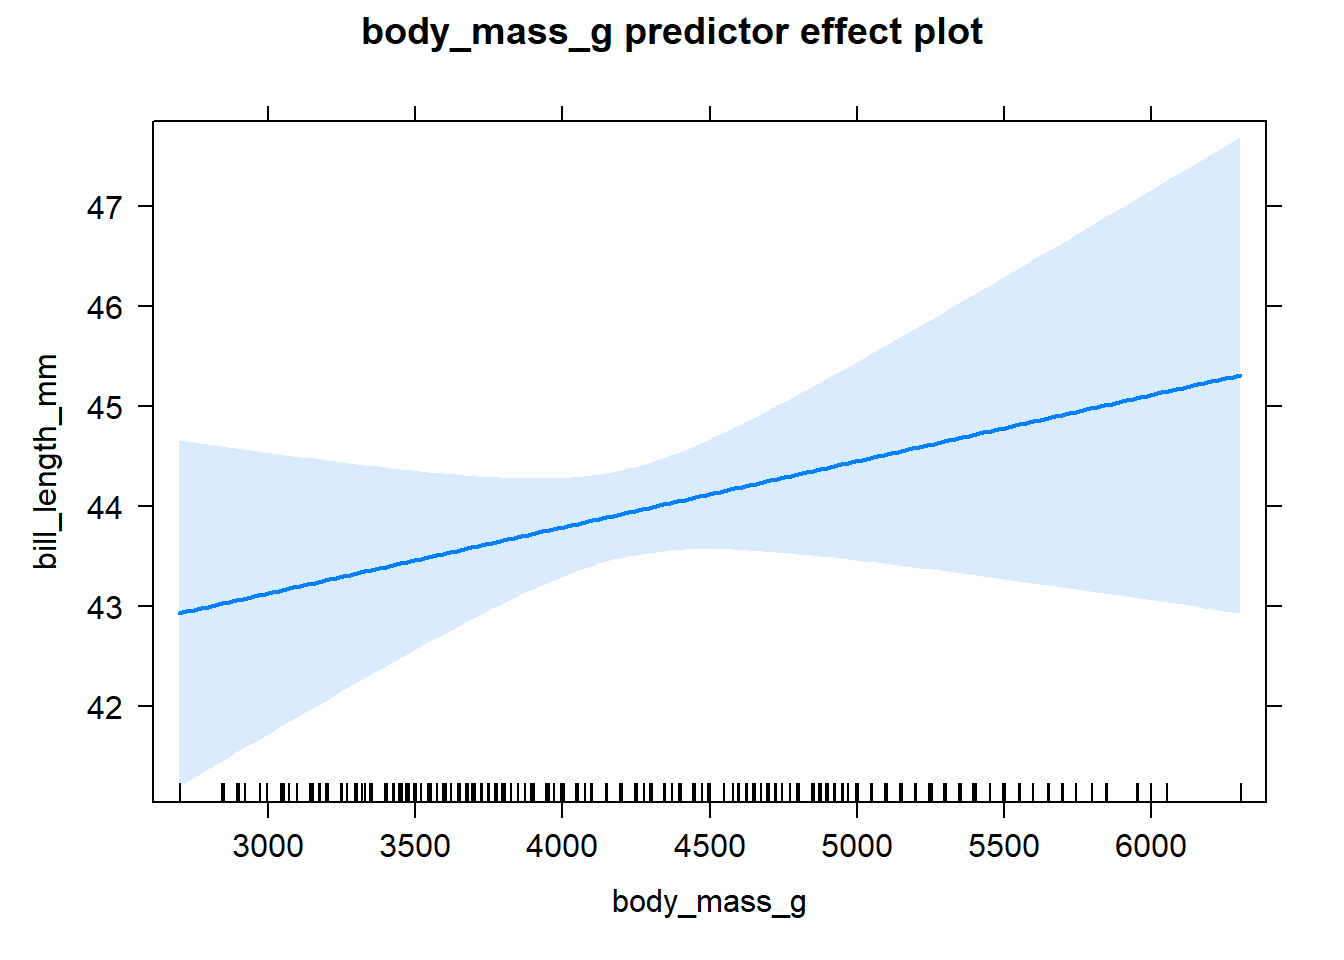
\includegraphics{A-Progessive-Introduction-to-Linear-Models_files/figure-latex/effect-plot-body-mass-1.pdf}
\caption{\label{fig:effect-plot-body-mass}Effect plot for body mass based on the fitted model in Equation \eqref{eq:mlr-effect-equation}.}
\end{figure}

We see from Figure \ref{fig:effect-plot-body-mass} that there is a
clear positive association between \texttt{body\_mass\_g} and \texttt{bill\_length\_mm}
after accounting for the \texttt{flipper\_length\_mm} variable. The shaded area
indicates the 95\% confidence interval bands for the estimated mean
response. We do not discuss confidence interval bands here, except to
say that they provide a visual picture of the uncertainty of our
estimated mean (wider bands indicate greater uncertainty). Chapter
\ref{inference} discusses confidence intervals for linear models in
some detail. The many tick marks along the the x-axis of the effect plot
indicate observed values of the x-axis variable.

We next create an effect plot for \texttt{flipper\_length\_mm}, which is shown in
Figure \ref{fig:effect-plot-flipper-length}, using the code below.
There is a clear positive association between \texttt{flipper\_length\_mm} and
\texttt{bill\_length\_mm} after accounting for \texttt{body\_mass\_g}.

\begin{Shaded}
\begin{Highlighting}[]
\CommentTok{\# draw effect plot for flipper\_length\_mm}
\FunctionTok{plot}\NormalTok{(}\FunctionTok{predictorEffect}\NormalTok{(}\StringTok{"flipper\_length\_mm"}\NormalTok{, mlmod))}
\end{Highlighting}
\end{Shaded}

\begin{figure}
\centering
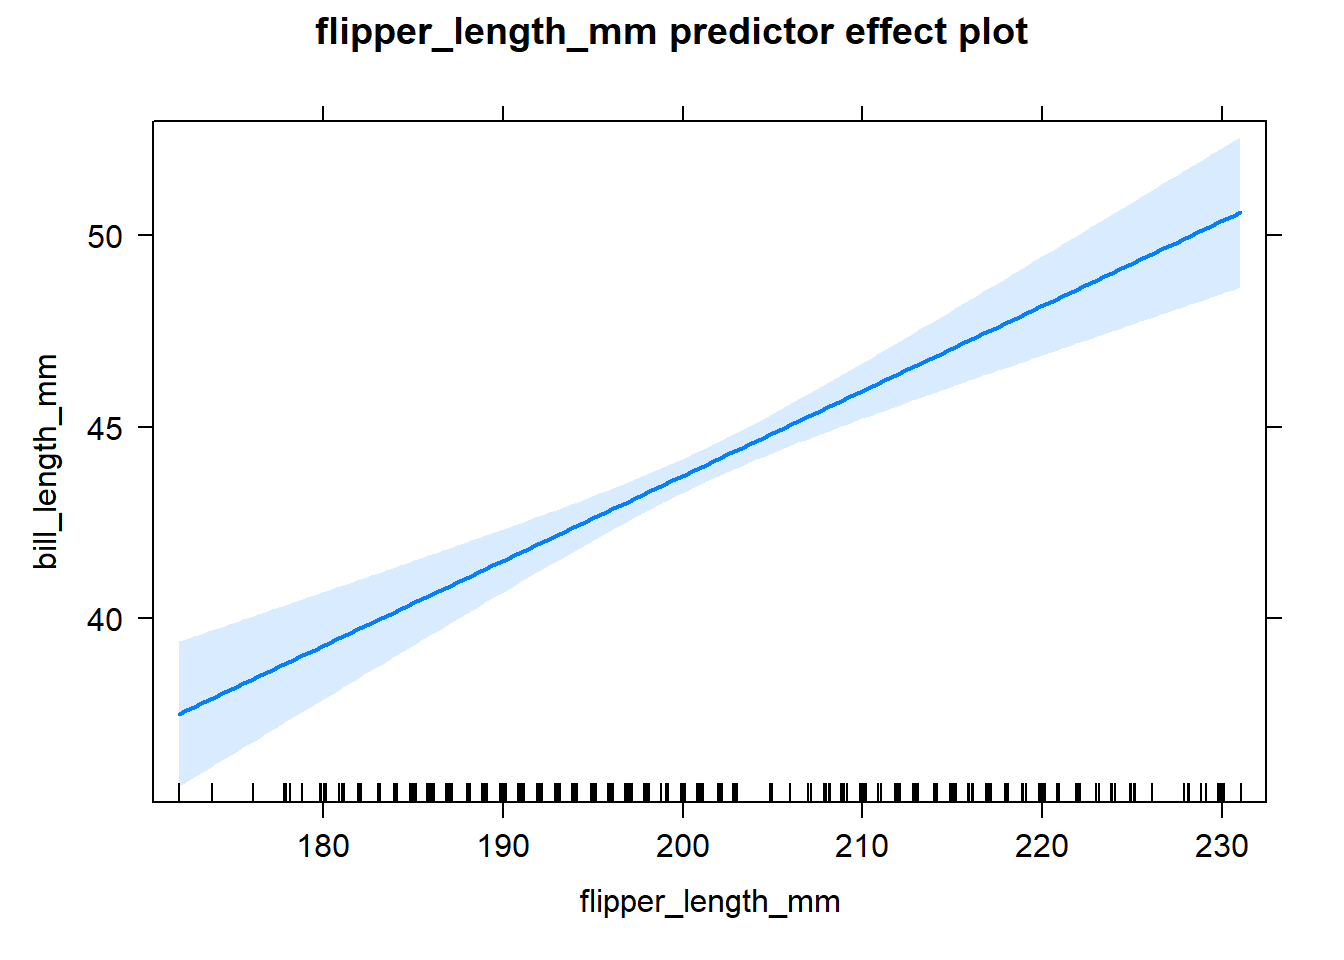
\includegraphics{A-Progessive-Introduction-to-Linear-Models_files/figure-latex/effect-plot-flipper-length-1.pdf}
\caption{\label{fig:effect-plot-flipper-length}Effect plot for flipper length based on the fitted model in Equation \eqref{eq:mlr-effect-equation}.}
\end{figure}

Alternatively, we could use \texttt{effects::allEffects} to compute the
necessary effect plot information for all predictors simultaneously,
then use \texttt{plot} to create a display of the effect plots for all
predictors in one graphic. This approach is quicker, but the individual
effect plots can sometimes be too small for practical use. We
demonstrate this faster approach in the code below, which produces
Figure \ref{fig:mlmod-effect-plots-all}.

\begin{Shaded}
\begin{Highlighting}[]
\FunctionTok{plot}\NormalTok{(}\FunctionTok{allEffects}\NormalTok{(mlmod))}
\end{Highlighting}
\end{Shaded}

\begin{figure}
\centering
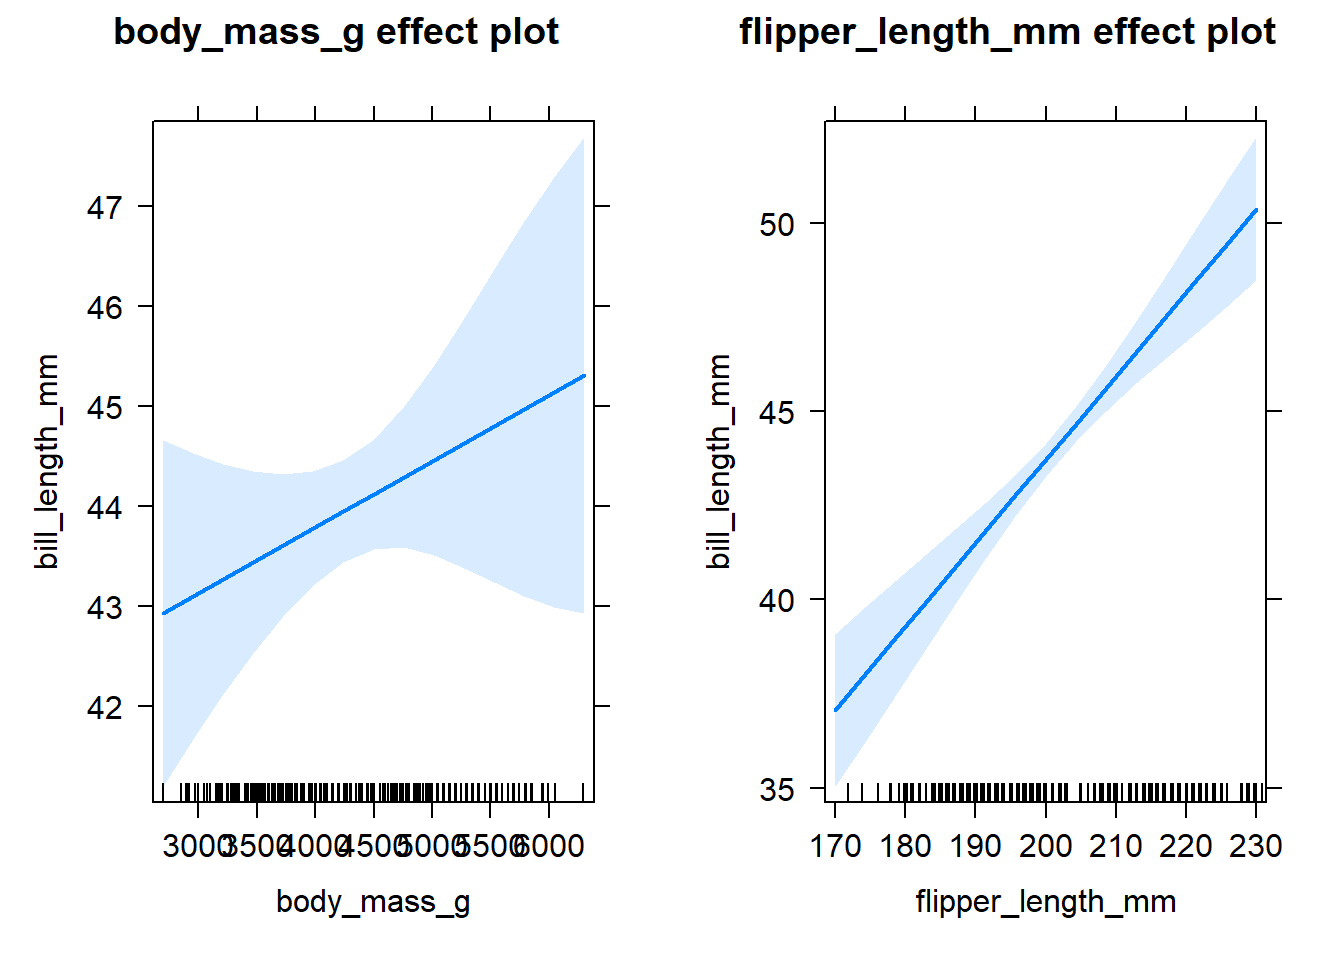
\includegraphics{A-Progessive-Introduction-to-Linear-Models_files/figure-latex/mlmod-effect-plots-all-1.pdf}
\caption{\label{fig:mlmod-effect-plots-all}All effect plots for predictors of the fitted model in Equation \eqref{eq:mlr-effect-equation}.}
\end{figure}

\hypertarget{interp-cat-predictor}{%
\section{Interpretation for categorical predictors}\label{interp-cat-predictor}}

We now discuss the interpretation of regression coefficients in the
context of a parallel lines and separate lines models.

\hypertarget{pl-interp}{%
\subsection{Coefficient interpretation for parallel lines models}\label{pl-interp}}

Consider a parallel lines model with numeric regressor \(X\) and
categorical predictor \(C\) with levels \(L_1\), \(L_2\), and \(L_3\). Following
the discussion in Section \ref{categorical-predictors}, predictor \(C\)
must be transformed into two indicator variables, \(D_2\) and \(D_3\), for
category levels \(L_2\) and \(L_3\), to be included in our linear model.
\(L_1\) is the reference level. The parallel lines model is formulated as
\[
E(Y \mid X, C) = \beta_{int} + \beta_{X} X + \beta_{L_2} D_2 +  \beta_{L_3} D_3, \label{eq:pl-def-interp}
\] where we replace the usual \(\beta_0\), \(\beta_1\), \(\beta_2\), and
\(\beta_3\) with notation the indicates the regressor each coefficient is
associated with.

When an observation has level \(L_1\) and \(X=0\), then the expected
response is \[
\begin{aligned}
E(Y|X = 0, C=L_1) &= \beta_{int} + \beta_X \cdot 0 + \beta_{L_2} \cdot 0 + \beta_{L_3} \cdot 0 \\
&= \beta_{int}.
\end{aligned}
\] Thus, \(\beta_{int}\) is the expected response for an observation with
level \(L_1\) when \(X=0\).

When an observation has a fixed level \(L_j\) (it doesn't matter which
level) and \(X\) increases from \(x^*\) to \(x^*+1\), then the change in the
expected response is \[
E(Y|X = x^* + 1, C=L_j) - E(Y|X = x^*, C=L_j)= \beta_X.
\] Thus, \(\beta_X\) is the expected change in the response for an
observation with fixed level \(L_j\) when \(X\) increases by 1 unit.

When an observation has level \(L_2\), the expected response is \[
\begin{aligned}
E(Y\mid X = x^*, C=L_2) &= \beta_{int} + \beta_X x^* + \beta_{L_2} \cdot 1 + \beta_{L_3} \cdot 0 \\
&= \beta_{int} + \beta_X x^* + \beta_{L_2}.
\end{aligned}
\] Thus, \[
\begin{aligned}
& E(Y\mid X=x^*, C=L_2) - E(Y\mid X=x^*, C=L_1) \\
&= (\beta_{int} + \beta_X x^* + \beta_{L_2}) - (\beta_{int} + \beta_X x^*) \\
&=  \beta_{L_2}.
\end{aligned}
\] Thus, \(\beta_{L_2}\) is the expected change in the response for a
fixed value of \(X\) when comparing on observation having level \(L_1\) to
level \(L_2\) of predictor \(C\). More specifically, \(\beta_{L_2}\) indicates
the distance between the estimated regression lines for observations
having levels \(L_1\) and \(L_2\). A similar interpretation holds for
\(\beta_{L_3}\) when comparing observations having level \(L_3\) to
observations having level \(L_1\). \(L_1\) is known as as the reference
level of \(C\) because we must refer to it to interpret our model with
respect to other levels of \(C\).

To summarize the interpretation of the coefficients in parallel lines
models like Equation \eqref{eq:pl-def-interp}, assuming categorical
predictor \(C\) has \(K\) levels instead of 3:

\begin{itemize}
\tightlist
\item
  \(\beta_{int}\) represents the expected response for observations
  having the reference level when the numeric regressor \(X = 0\).
\item
  \(\beta_X\) is the expected change in the response when \(X\) increases
  by 1 unit for a fixed level of \(C\).
\item
  \(\beta_{L_j}\), for \(j=2,\ldots,K\), represents the expected change in
  the response when comparing observations having level \(L_1\) and
  \(L_j\) with \(X\) fixed at the same value.
\end{itemize}

In Section \ref{s:penguins-mlr2}, we fit a parallel lines model to the
\texttt{penguins} data that used both \texttt{body\_mass\_g} and \texttt{species} to explain
the behavior of \texttt{bill\_length\_mm}. Letting \(D_C\) denote the indicator
variable for the \texttt{Chinstrap} level and \(D_G\) denote the indicator
variable for the \texttt{Gentoo} level, the fitted parallel lines model was \[
\begin{aligned}
&\hat{E}(\mathtt{bill\_length\_mm} \mid \mathtt{body\_mass\_g}, \mathtt{species})\\
&= 24.92 + 0.004 \mathtt{body\_mass\_g} + 9.92 D_C + 3.56 D_G.
\end{aligned}
\] In the context of this model:

\begin{itemize}
\tightlist
\item
  The expected bill length for an Adelie penguin with a body mass of 0
  grams is 24.92 mm.
\item
  If two penguins are of the same species, but one penguin has a body
  mass 1 gram larger, then the larger penguin is expected to have a
  bill length 0.004 mm longer than the smaller penguin.
\item
  A Chinstrap penguin is expected to have a bill length 9.92 mm longer
  than an Adelie penguin, assuming their body mass is the same.
\item
  A Gentoo penguin is expected to have a bill length 3.56 mm longer
  than an Adelie penguin, assuming their body mass is the same.
\end{itemize}

\hypertarget{effect-plots-for-fitted-models-with-non-interacting-categorical-predictors}{%
\subsection{Effect plots for fitted models with non-interacting categorical predictors}\label{effect-plots-for-fitted-models-with-non-interacting-categorical-predictors}}

How do we create an effect plot for a numeric focal predictor when a
non-interacting categorical predictor is in the model (such as for the
parallel lines model we have been discussing)? In short, we determine
the fitted model equation as a function of the focal predictor for each level of
the categorical predictor, and then compute the weighted average of the
equation with the weights being proportional to the number of
observations in each group.

Let's construct an effect plot for the \texttt{body\_mass\_g} predictor in the
context of the \texttt{penguins} parallel lines model discussed in the previous
section. In Section \ref{s:penguins-mlr2}, we determined that the
fitted parallel lines model simplified to the following equations
depending on the level of \texttt{species}: \[
\begin{aligned}
&\hat{E}(\mathtt{bill\_length\_mm} \mid \mathtt{body\_mass\_g}, \mathtt{species}=\mathtt{Adelie}) \\
&= 24.92 + 0.004 \mathtt{body\_mass\_g} \\
&\hat{E}(\mathtt{bill\_length\_mm} \mid \mathtt{body\_mass\_g}, \mathtt{species}=\mathtt{Chinstrap}) \\
&= 34.84 + 0.004 \mathtt{body\_mass\_g} \\
&\hat{E}(\mathtt{bill\_length\_mm} \mid \mathtt{body\_mass\_g}, \mathtt{species}=\mathtt{Gentoo}) \\
&= 28.48 + 0.004 \mathtt{body\_mass\_g}.
\end{aligned}
\label{eq:pl-equations}
\] We recreate the fitted model producing these equations in R using the
code below.

\begin{Shaded}
\begin{Highlighting}[]
\CommentTok{\# refit the parallel lines model}
\NormalTok{lmodp }\OtherTok{\textless{}{-}} \FunctionTok{lm}\NormalTok{(bill\_length\_mm }\SpecialCharTok{\textasciitilde{}}\NormalTok{ body\_mass\_g }\SpecialCharTok{+}\NormalTok{ species, }\AttributeTok{data =}\NormalTok{ penguins)}
\CommentTok{\# double{-}check coefficients}
\FunctionTok{coef}\NormalTok{(lmodp)}
\DocumentationTok{\#\#      (Intercept)      body\_mass\_g speciesChinstrap }
\DocumentationTok{\#\#     24.919470977      0.003748497      9.920884113 }
\DocumentationTok{\#\#    speciesGentoo }
\DocumentationTok{\#\#      3.557977539}
\end{Highlighting}
\end{Shaded}

The code below determines the number of observations with each level of
\texttt{species} for the data used in the fitted model \texttt{lmodp}. We see that 151
Adelie, 68 Chinstrap, and 123 Gentoo penguins (342 total penguins) were
used to fit the model stored in \texttt{lmodp}.

\begin{Shaded}
\begin{Highlighting}[]
\FunctionTok{table}\NormalTok{(lmodp}\SpecialCharTok{$}\NormalTok{model}\SpecialCharTok{$}\NormalTok{species)}
\DocumentationTok{\#\# }
\DocumentationTok{\#\#    Adelie Chinstrap    Gentoo }
\DocumentationTok{\#\#       151        68       123}
\end{Highlighting}
\end{Shaded}

The equation used to create the effect plot of \texttt{body\_mass\_g} is the
weighted average of the equations in Equation \eqref{eq:pl-equations},
with weights proportional to the number of observational having each
level of the categorical predictor. Specifically, \[
\begin{aligned}
& \hat{E}(\mathtt{bill\_length\_mm} \mid \mathtt{body\_mass\_g}, \mathtt{species}=\mathtt{typical}) \\
&= \frac{151}{342}(24.92 + 0.004 \mathtt{body\_mass\_g})\\
&\quad + \frac{68}{342}(34.84 + 0.004 \mathtt{body\_mass\_g})\\
&\quad + \frac{123}{342}(28.48 + 0.004 \mathtt{body\_mass\_g}) \\
&=28.17 + 0.004 \mathtt{body\_mass\_g}.
\end{aligned}
\] The effect plot for \texttt{body\_mass\_g} for the fitted parallel lines model
is shown in Figure \ref{fig:effect-plot-plmod-body-mass}. The
association between \texttt{bill\_length\_mm} and \texttt{body\_mass\_g} is positive after
accounting for \texttt{species}.

\begin{Shaded}
\begin{Highlighting}[]
\CommentTok{\# draw effect plot for body\_mass\_g}
\FunctionTok{plot}\NormalTok{(}\FunctionTok{predictorEffect}\NormalTok{(}\StringTok{"body\_mass\_g"}\NormalTok{, lmodp))}
\end{Highlighting}
\end{Shaded}

\begin{figure}
\centering
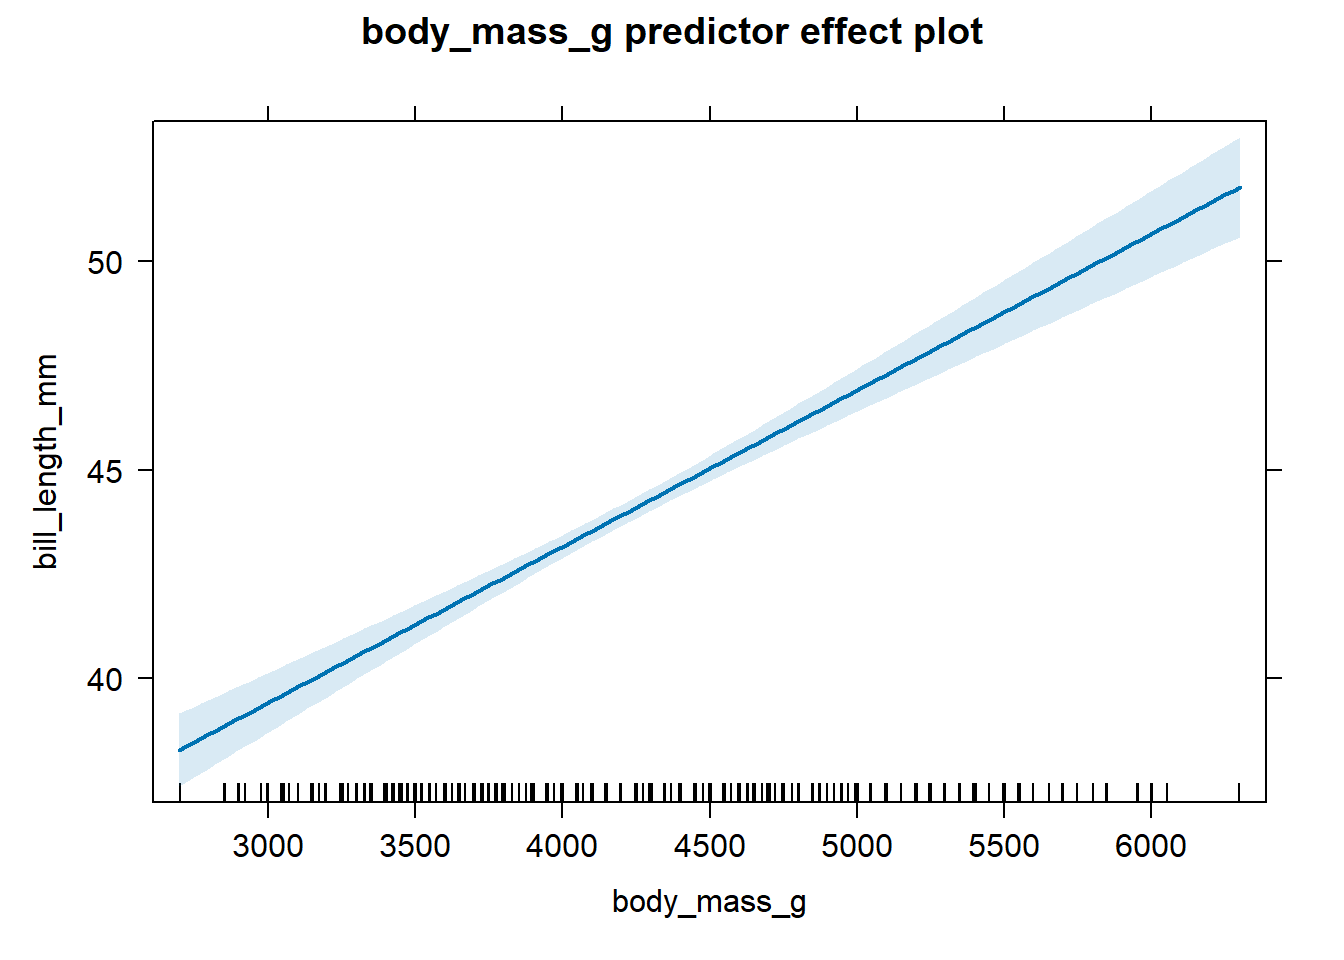
\includegraphics{A-Progessive-Introduction-to-Linear-Models_files/figure-latex/effect-plot-plmod-body-mass-1.pdf}
\caption{\label{fig:effect-plot-plmod-body-mass}The effect plot of \texttt{body\_mass\_g} for the fitted parallel lines model.}
\end{figure}

An effect plot for a categorical predictor, assuming all other
predictors in the model are non-interacting numerical predictors (i.e.,
fixed group predictors), is a plot of the estimated mean response for
each level of the categorical variable when the fixed group group
predictors are held at their sample mean. The sample mean of the
\texttt{body\_mass\_g} values used to fit \texttt{lmodp} is 4201.75, as shown in the
code below.

\begin{Shaded}
\begin{Highlighting}[]
\CommentTok{\# sample mean of body\_mass\_g variable used to fit lmodp}
\FunctionTok{mean}\NormalTok{(lmodp}\SpecialCharTok{$}\NormalTok{model}\SpecialCharTok{$}\NormalTok{body\_mass\_g)}
\DocumentationTok{\#\# [1] 4201.754}
\end{Highlighting}
\end{Shaded}

Using the first equation in Equation \eqref{eq:pl-equations}, the
estimated mean for the Adelie species when \texttt{body\_mass\_g} is fixed at
4201.75 is \[
\begin{aligned}
&\hat{E}(\mathtt{bill\_length\_mm} \mid \mathtt{body\_mass\_g} = 4201.75, \mathtt{species}=\mathtt{Adelie}) \\
&= 24.92 + 0.004 \cdot 4201.75 \\
&= 40.67.
\end{aligned}
\] Similarly,
\(\hat{E}(\mathtt{bill\_length\_mm} \mid \mathtt{body\_mass\_g} = 4201.75, \mathtt{species}=\mathtt{Chinstrap}) = 50.59\)
and
\(\hat{E}(\mathtt{bill\_length\_mm} \mid \mathtt{body\_mass\_g} = 4201.75, \mathtt{species}=\mathtt{Gentoo}) = 44.23\).

The code below produces the effect plot for \texttt{species}, which is shown in
Figure \ref{fig:eff-plot-species-plmod}. We see that after accounting
for \texttt{body\_mass\_g}, the \texttt{bill\_length\_mm} tends to be largest for
Chinstrap penguins, second largest for Gentoo penguins, and smallest for
Adelie penguins. The confidence bands for the estimated mean response
are shown by the vertical bars.

\begin{Shaded}
\begin{Highlighting}[]
\FunctionTok{plot}\NormalTok{(}\FunctionTok{predictorEffect}\NormalTok{(}\StringTok{"species"}\NormalTok{, lmodp))}
\end{Highlighting}
\end{Shaded}

\begin{figure}
\centering
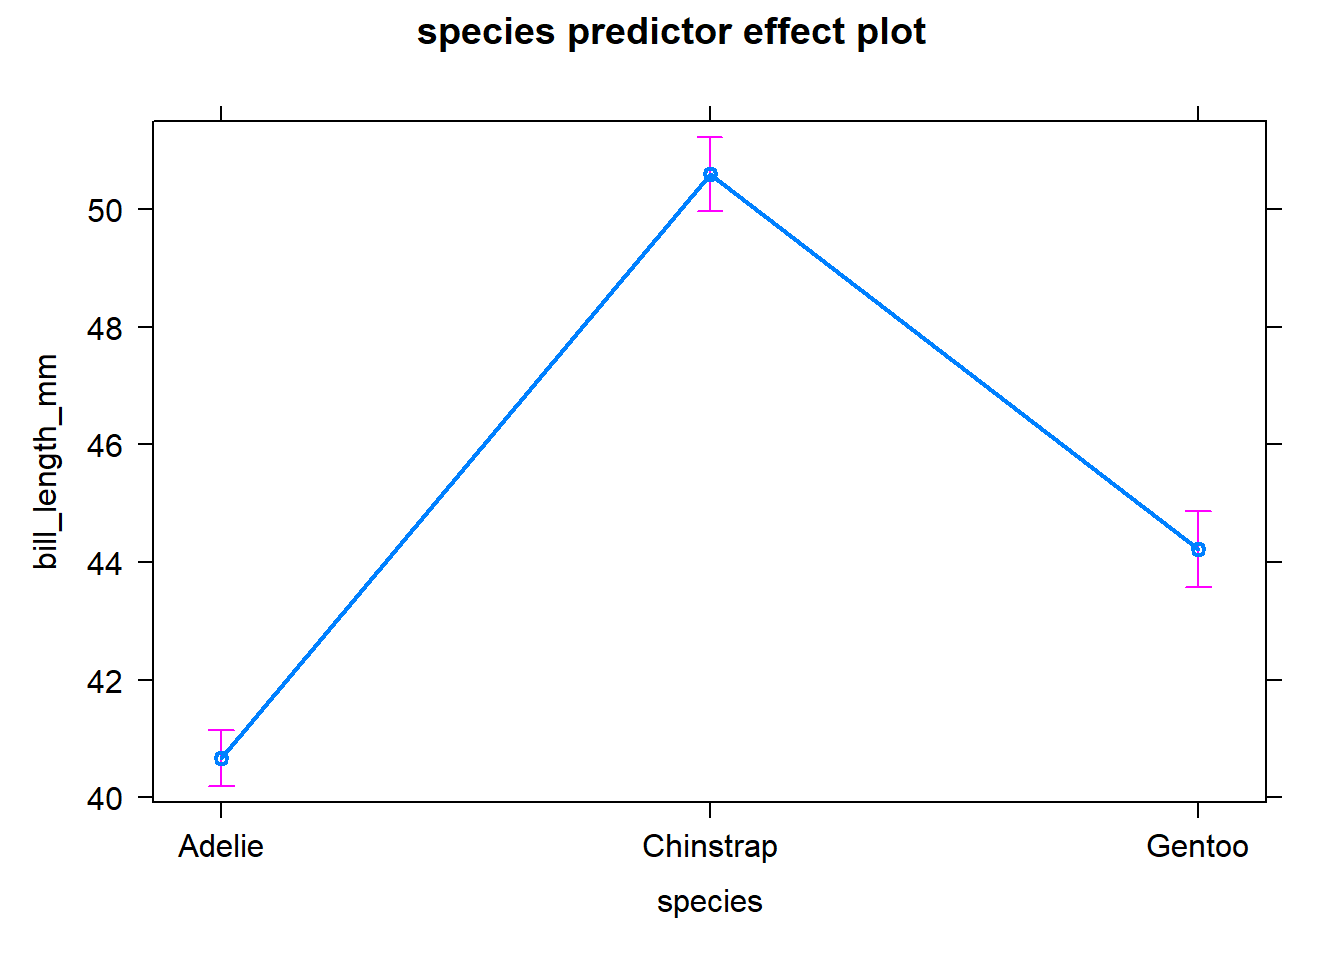
\includegraphics{A-Progessive-Introduction-to-Linear-Models_files/figure-latex/eff-plot-species-plmod-1.pdf}
\caption{\label{fig:eff-plot-species-plmod}An effect plot for \texttt{species} after accounting for \texttt{body\_mass\_g}.}
\end{figure}

\hypertarget{sl-interp}{%
\subsection{Coefficient interpretation for separate lines models}\label{sl-interp}}

Consider a separate lines model with numeric regressor \(X\) and
categorical predictor \(C\) with levels \(L_1\), \(L_2\), and \(L_3\). The
predictor \(C\) will be transformed into two indicator variables, \(D_2\)
and \(D_3\), for category levels \(L_2\) and \(L_3\), with \(L_1\) being the
reference level. The separate lines model is formulated as \[
E(Y \mid X, C) = \beta_{int} + \beta_{X} X + \beta_{L_2} D_2 +  \beta_{L_3} D_3 + \beta_{XL_2} XD_2+\beta_{XL_3}XD_3. \label{eq:sl-def-interp}
\]

When an observation has level \(L_1\) and \(X=x^*\), then the expected
response is \[
\begin{aligned}
&E(Y\mid X = x^*, C=L_1) \\
&= \beta_{int} + \beta_X \cdot x^* + \beta_{L_2} \cdot 0 + \beta_{L_3} \cdot 0  + \beta_{X L_2} \cdot x^* \cdot 0 + \beta_{X L_3}\cdot x^* \cdot 0 \\
&= \beta_{int} + \beta_X x^*.
\end{aligned}
\label{eq:slr-mean-L1}
\]

Using Equation \eqref{eq:slr-mean-L1}, we can verify that:

\begin{itemize}
\tightlist
\item
  \(\beta_{int} = E(Y\mid X = 0, C=L_1)\).
\item
  \(\beta_{X} = E(Y\mid X = x^* + 1, C=L_1) - E(Y\mid X = x^*, C=L_1)\).
\end{itemize}

Similarly, when \(C=L_2\), \[
\begin{aligned}
& E(Y|X = x^*, C=L_2) \\
&= \beta_{int} + \beta_X \cdot x^* + \beta_{L_2} \cdot 1 + \beta_{L_3} \cdot 0  + \beta_{X L_2} \cdot x^* \cdot 1 + \beta_{X L_3}\cdot x^* \cdot 0 \\
&= \beta_{int} + \beta_X x^* + \beta_{L_2} + \beta_{XL_2}x^*\\
&= (\beta_{int} + \beta_{L_2}) + (\beta_X + \beta_{XL_2})x^*.
\end{aligned}
\label{eq:slr-mean-L2}
\] Following this same pattern, when \(C=L_3\) we have \[
E(Y|X = x^*, C=L_3) = (\beta_{int} + \beta_{L_3}) + (\beta_X + \beta_{XL_3})x^*. \label{eq:slr-mean-L3}
\]

Using Equations \eqref{eq:slr-mean-L1}, \eqref{eq:slr-mean-L2}, and
\eqref{eq:slr-mean-L3}, we can verify that for \(j=2,3\),
\[\beta_{L_j}= E(Y\mid X = 0, C=L_j) - E(Y\mid X = 0, C=L_1),\] and \[
\begin{aligned}
& \beta_{XL_j} \\
&= [E(Y\mid X = x^*+1, C=L_j) - E(Y\mid X = x^*, C=L_j)]\\
&\quad-[E(Y\mid X = x^*+1, C=L_1) - E(Y\mid X = x^*, C=L_1)].
\end{aligned}
\]

To summarize the interpretation of the coefficients in separate lines
models like Equation \eqref{eq:sl-def-interp}, assuming categorical
predictor \(C\) has \(K\) levels instead of 3:

\begin{itemize}
\tightlist
\item
  \(\beta_{int}\) represents the expected response for observations
  having the reference level when the numeric regressor \(X = 0\).
\item
  \(\beta_{L_j}\), for \(j=2,\ldots,K\), represents the expected change in
  the response when comparing observations having level \(L_1\) and
  \(L_j\) with \(X=0\).
\item
  \(\beta_X\) represents the expected change in the response when \(X\)
  increases by 1 unit for observations having the reference level.
\item
  \(\beta_X L_j\), for \(j=2,\ldots,K\), represents the difference in the
  expected response between observations having the reference level in
  comparison to level \(L_j\) when \(X\) increases by 1 unit. More simply,
  these terms represent the difference in the rate of change for
  observations having level \(L_j\) compared to the reference level.
\end{itemize}

We illustrate these interpretation using the separate lines model to the
\texttt{penguins} data in Section \ref{s:penguins-mlr2}. The fitted
separate lines model was \[
\begin{aligned}
&\hat{E}(\mathtt{bill\_length\_mm} \mid \mathtt{body\_mass\_g}, \mathtt{species}) \\
&= 26.99 + 0.003 \mathtt{body\_mass\_g} + 5.18 D_C - 0.25 D_G \\
&\quad + 0.001 D_C \mathtt{body\_mass\_g} + 0.0009 D_G \mathtt{body\_mass\_g}.
\end{aligned}
\label{eq:sl-refit-interp}
\] In the context of this model:

\begin{itemize}
\tightlist
\item
  The expected bill length for an Adelie penguin with a body mass of 0
  grams is 26.99 mm.
\item
  If an Adelie penguin has a body mass 1 gram larger than another
  Adelie penguin, then the larger penguin is expected to have a bill
  length 0.003 mm longer than the smaller penguin.
\item
  A Chinstrap penguin is expected to have a bill length 5.18 mm longer
  than an Adelie penguin when both have a body mass of 0 grams.
\item
  A Gentoo penguin is expected to have a bill length 0.25 mm shorter
  than an Adelie penguin when both have a body mass of 0 grams.
\item
  For each 1 gram increase in body mass, we expect the change in bill
  length by Chinstrap penguins to be 0.001 mm larger than the
  corresponding change in bill length by Adelie penguins.
\item
  For each 1 gram increase in body mass, we expect the change in bill
  length by Gentoo penguins to be 0.0009 mm larger than the
  corresponding change in bill length by Adelie penguins.
\end{itemize}

\hypertarget{effect-plots-for-interacting-categorical-predictors}{%
\subsection{Effect plots for interacting categorical predictors}\label{effect-plots-for-interacting-categorical-predictors}}

We now discuss construction of effect plots for a separate lines model,
which has an interaction between a categorical and numeric predictor. In
additional to the focal and fixed group predictors we have previously
discussed, Fox and Weisberg (\protect\hyperlink{ref-fox2020predictor}{2020}) also discuss predictors in the
\textbf{conditioning group}, which is the set of predictors that interact
with the focal predictor.

When some predictors interact with the focal predictor, the effect plot
of the focal predictor is a plot of the estimated mean response when the
fixed group predictors are held at their typical values and the
conditioning group predictors vary over different combinations of
discrete values. The process of determining the estimated mean response
as function of the focal predictor is similar to before, but there are
more predictor values on which to condition. By default, to compute the
estimated mean response as a function of the focal predictor, we:

\begin{itemize}
\tightlist
\item
  Hold the numeric fixed group predictors at their sample means.
\item
  Average the estimated mean response equation across the different
  levels of a fixed group categorical predictor, with weights equal to
  the number of observations with each level.
\item
  Compute the estimated mean response function for 5 discrete
  values of numeric predictors in the conditioning group.
\item
  Compute the estimated mean response function for different levels
  of a categorical predictor in the conditioning group.
\end{itemize}

We provide examples of the effect plots for the \texttt{body\_mass\_g} and
\texttt{species} predictors for the separate lines model fit to the \texttt{penguins}
data and given in Equation \eqref{eq:sl-refit-interp}. We first run the
code below to fit the separate lines model previously fit in Section
\ref{s:penguins-mlr2}.

\begin{Shaded}
\begin{Highlighting}[]
\CommentTok{\# fit separate lines model}
\NormalTok{lmods }\OtherTok{\textless{}{-}} \FunctionTok{lm}\NormalTok{(bill\_length\_mm }\SpecialCharTok{\textasciitilde{}}\NormalTok{ body\_mass\_g }\SpecialCharTok{+}\NormalTok{ species }\SpecialCharTok{+}\NormalTok{ body\_mass\_g}\SpecialCharTok{:}\NormalTok{species,}
            \AttributeTok{data =}\NormalTok{ penguins)}
\CommentTok{\# extract estimated coefficients}
\FunctionTok{coef}\NormalTok{(lmods)}
\DocumentationTok{\#\#                  (Intercept)                  body\_mass\_g }
\DocumentationTok{\#\#                26.9941391367                 0.0031878758 }
\DocumentationTok{\#\#             speciesChinstrap                speciesGentoo }
\DocumentationTok{\#\#                 5.1800537287                {-}0.2545906615 }
\DocumentationTok{\#\# body\_mass\_g:speciesChinstrap    body\_mass\_g:speciesGentoo }
\DocumentationTok{\#\#                 0.0012748183                 0.0009029956}
\end{Highlighting}
\end{Shaded}

We previously determined in Section \ref{s:penguins-mlr2} that the
model simplifies depending on the level of species. Specifically, we
have that \[
\begin{aligned}
&\hat{E}(\mathtt{bill\_length\_mm} \mid \mathtt{body\_mass\_g}, \mathtt{species}=\mathtt{Adelie}) \\
&= 26.99 + 0.003 \mathtt{body\_mass\_g},\\
&\hat{E}(\mathtt{bill\_length\_mm} \mid \mathtt{body\_mass\_g}, \mathtt{species}=\mathtt{Chinstrap}) \\
&= 31.17 + 0.004 \mathtt{body\_mass\_g},\\
&\hat{E}(\mathtt{bill\_length\_mm} \mid \mathtt{body\_mass\_g}, \mathtt{species}=\mathtt{Chinstrap}) \\
&= 26.74 + 0.004 \mathtt{body\_mass\_g}.
\end{aligned}
\label{eq:separate-lines-equations-effects-plot}
\]

The effect plot of \texttt{body\_mass\_g} for the separate lines model will be a
plot of each equation given in Equation
\eqref{eq:separate-lines-equations-effects-plot}. Figure
\ref{fig:effect-plot-body-mass-lmods} displays this effect plot, which
was created using the code below. We use the \texttt{axes} argument to rotate
the x-axis labels (otherwise the text overlaps) and the \texttt{lines}
argument to display all three lines in one graphic instead of a
separate panel for each level of \texttt{species}. We notice Chinstrap penguins
tend to have the largest bill lengths for a given value of body mass and
the bill lengths increase more quickly as a function of body mass then
for the Adelie and Gentoo penguins. Similarly, the Adelie penguins tend
to have the smallest bill length for a fixed value of body mass and the
bill length tends to increase more slowly as body mass increases
compared to the other two types of penguins.

\begin{Shaded}
\begin{Highlighting}[]
\CommentTok{\# effect plot of body mass for separate lines model}
\CommentTok{\# axes ... rotates the x{-}axis labels 90 degrees}
\CommentTok{\# lines ... plots the effect of body mass in one graphic}
\FunctionTok{plot}\NormalTok{(}\FunctionTok{predictorEffect}\NormalTok{(}\StringTok{"body\_mass\_g"}\NormalTok{, lmods),}
     \AttributeTok{axes =} \FunctionTok{list}\NormalTok{(}\AttributeTok{x =} \FunctionTok{list}\NormalTok{(}\AttributeTok{rotate =} \DecValTok{90}\NormalTok{)),}
     \AttributeTok{lines =} \FunctionTok{list}\NormalTok{(}\AttributeTok{multiline =} \ConstantTok{TRUE}\NormalTok{))}
\end{Highlighting}
\end{Shaded}

\begin{figure}
\centering
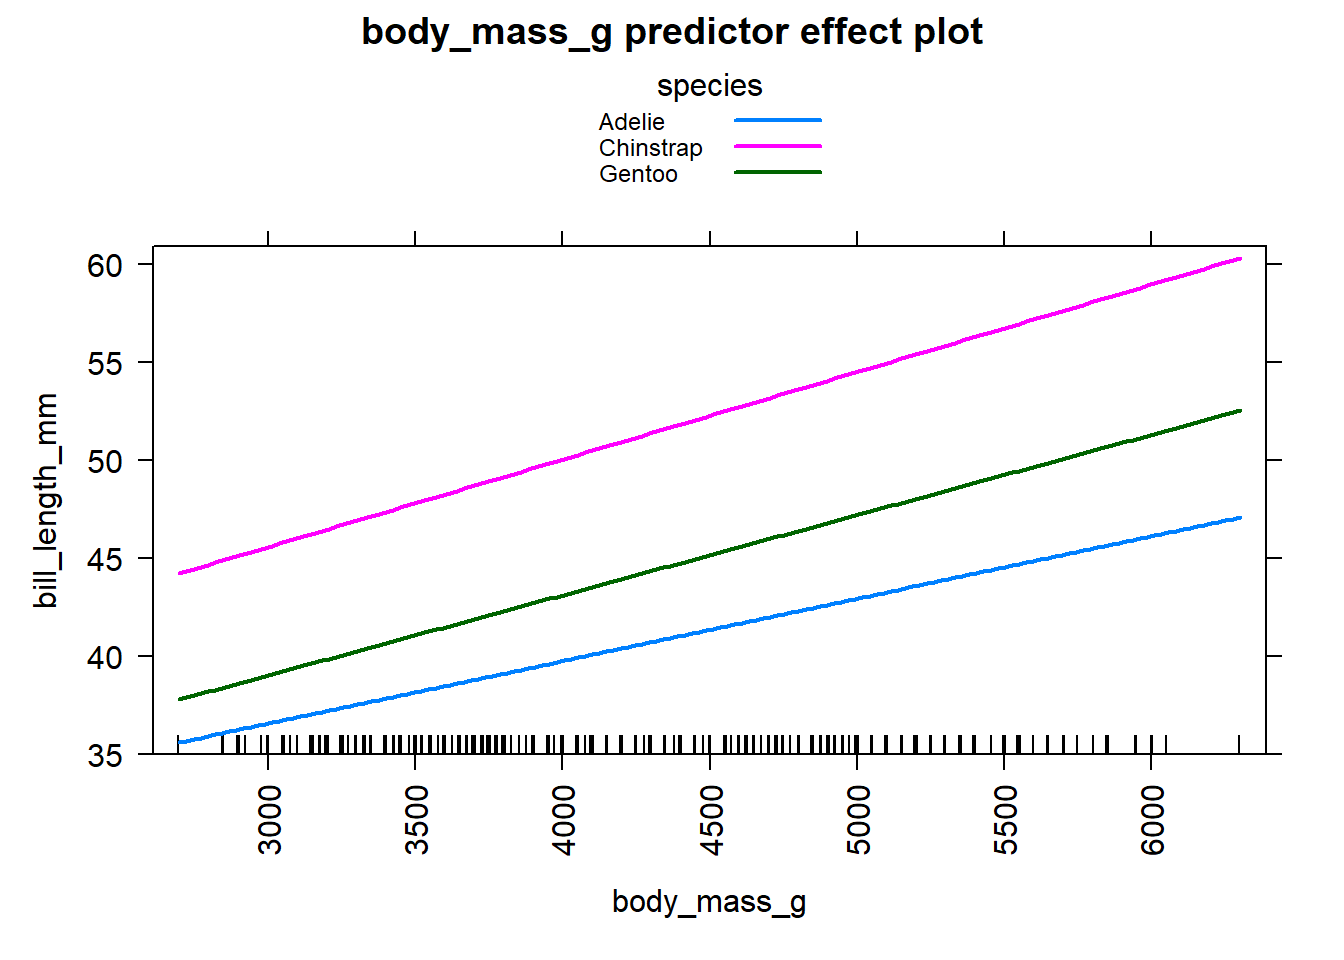
\includegraphics{A-Progessive-Introduction-to-Linear-Models_files/figure-latex/effect-plot-body-mass-lmods-1.pdf}
\caption{\label{fig:effect-plot-body-mass-lmods}Effect plot for body mass based on the equations in Equation \eqref{eq:separate-lines-equations-effects-plot}.}
\end{figure}

The effect plot of \texttt{species} for the separate lines model will be a plot
of the estimated mean response in Equation
\eqref{eq:separate-lines-equations-effects-plot} for each level of
\texttt{species} when varying \texttt{body\_mass\_g} over 5 discrete values. Figure
\ref{fig:effect-plot-species-lmods} displays this effect plot, which
was created using the code below. By specifying
\texttt{lines\ =\ list(multiline\ =\ TRUE)}, the estimated mean responses for each
level of \texttt{species} are connected for each discrete value of
\texttt{body\_mass\_g}. Figure \ref{fig:effect-plot-species-lmods} allows us to
determine the effect of \texttt{species} on \texttt{bill\_length\_mm} when we vary
\texttt{body\_mass\_g} over 5 discrete values. When varying \texttt{body\_mass\_g} across
the values 2700, 3600, 4500, 5300, and 6300 g, we see greater changes in
the estimated mean of \texttt{bill\_lengh\_mm} for Chinstrap penguins in
comparison to Adelie and Gentoo penguins.

\begin{Shaded}
\begin{Highlighting}[]
\CommentTok{\# effect plot of body mass for separate lines model}
\CommentTok{\# axes ... rotates the x{-}axis labels 90 degrees}
\CommentTok{\# lines ... plots the effect of species in one graphic}
\FunctionTok{plot}\NormalTok{(}\FunctionTok{predictorEffect}\NormalTok{(}\StringTok{"species"}\NormalTok{, lmods),}
     \AttributeTok{axes =} \FunctionTok{list}\NormalTok{(}\AttributeTok{x =} \FunctionTok{list}\NormalTok{(}\AttributeTok{rotate =} \DecValTok{90}\NormalTok{)),}
     \AttributeTok{lines=}\FunctionTok{list}\NormalTok{(}\AttributeTok{multiline =} \ConstantTok{FALSE}\NormalTok{))}
\end{Highlighting}
\end{Shaded}

\begin{figure}
\centering
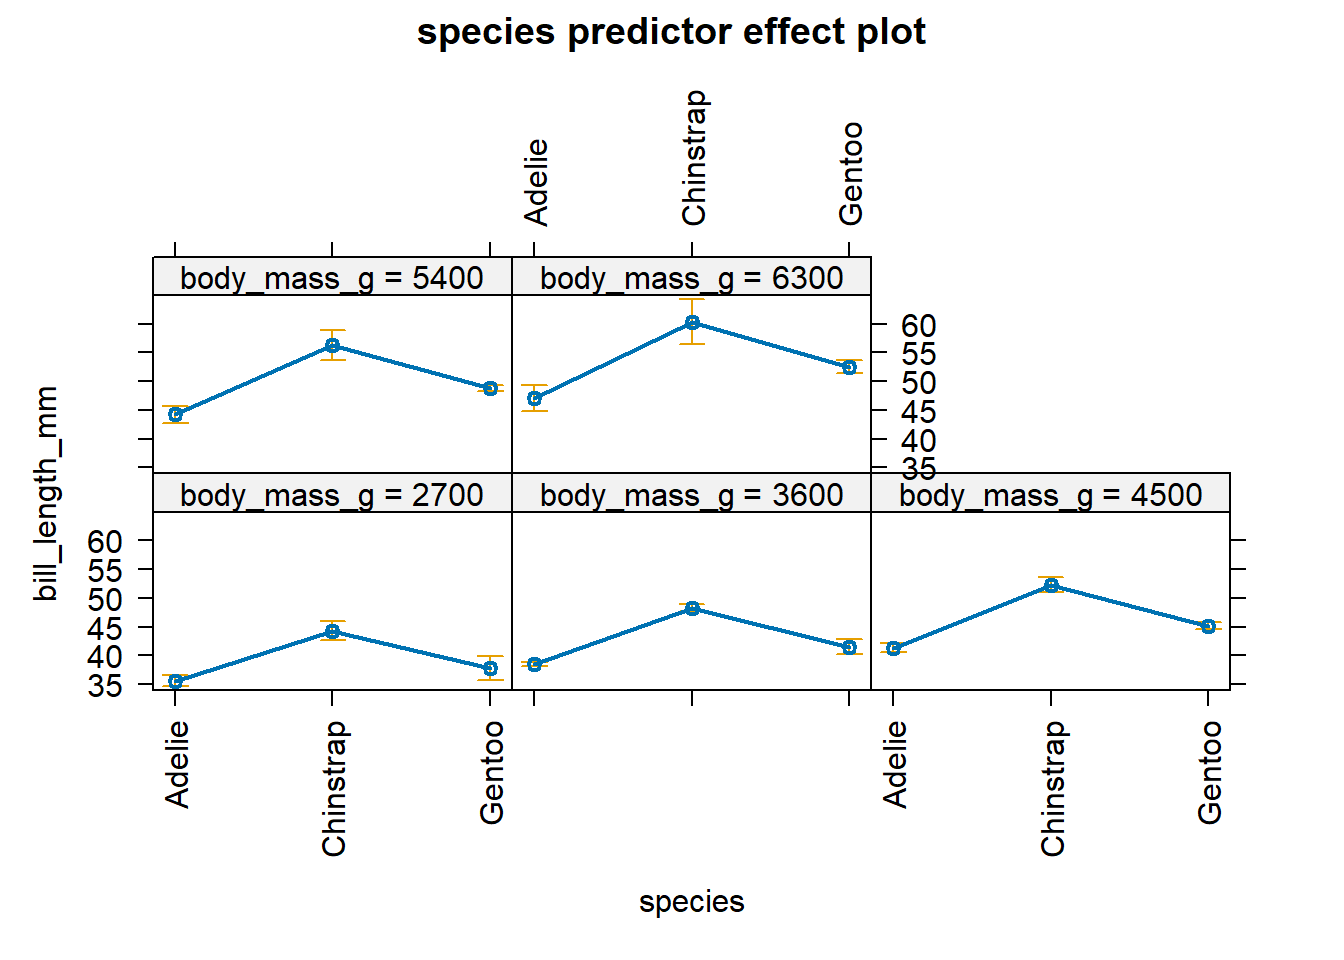
\includegraphics{A-Progessive-Introduction-to-Linear-Models_files/figure-latex/effect-plot-species-lmods-1.pdf}
\caption{\label{fig:effect-plot-species-lmods}Effect plot for species based on the equations in Equation \eqref{eq:separate-lines-equations-effects-plot}.}
\end{figure}

We refer the reader to the ``Predictor effects gallery'' vignette in the
\textbf{\texttt{effects}} package (run
\texttt{vignette("predictor-effects-gallery",\ package\ =\ "effects")} in the
Console) for more details about how to construct effect plots in
different settings.

\hypertarget{added-variable-and-leverage-plots}{%
\section{Added-variable and leverage plots}\label{added-variable-and-leverage-plots}}

An \textbf{added-variable plot} or \textbf{partial regression plot} displays the
marginal effect of a regressor on the response after accounting for the
other regressors in the model (\protect\hyperlink{ref-mt1977}{Mosteller and Tukey 1977}). While an effect plot is a plot
of the estimated mean relationship between the response and a focal
predictor while holding the model's predictors at typical values, the
added-variable plot is a plot of two sets of residuals against one
other.

We create an added-variable plot for regressor \(X_j\) in the following
way:

\begin{enumerate}
\def\labelenumi{\arabic{enumi}.}
\tightlist
\item
  Compute the residuals of the model regressing the response \(Y\) on
  all regressors except \(X_j\). We denote these residuals
  \(\hat{\boldsymbol{\epsilon}}(Y\mid \mathbb{X}_{-j})\). These
  residuals represent the part of the response variable not explained
  by the regressors in \(\mathbb{X}_{-j}\).
\item
  Compute the residuals of the model regressing the regressor \(X_j\) on
  all regressors except \(X_j\). We denote these residuals
  \(\hat{\boldsymbol{\epsilon}}(X_j \mid \mathbb{X}_{-j})\). These
  residuals represent the part of the \(X_j\) not explained by the
  regressors in \(\mathbb{X}_{-j}\). Alternatively, these residuals
  represent the amount of additional information \(X_j\) provides after
  accounting for the regressors in \(\mathbb{X}_{-j}\).
\item
  The added-variable plot for \(X_j\) is a plot of
  \(\hat{\boldsymbol{\epsilon}}(Y\mid \mathbb{X}_{-j})\) on the y-axis
  and \(\hat{\boldsymbol{\epsilon}}(X_j \mid \mathbb{X}_{-j})\) on the
  x-axis.
\end{enumerate}

Added-variable plots allow us to visualize the impact a regressor has
when added to an existing regression model. We can use the
added-variable plot for \(X_j\) to visually estimate the partial slope
\(\hat{\beta}_{j}\) (\protect\hyperlink{ref-sheather2009modern}{Sheather 2009}). In fact, the simple linear
regression line that minimizes the RSS for the added-variable plot of
\(X_j\) will have slope \(\hat{\beta}_j\).

We can use an added-variable plot in several ways:

\begin{enumerate}
\def\labelenumi{\arabic{enumi}.}
\tightlist
\item
  To assess the marginal relationship between \(X_j\) and \(Y\) after
  accounting for all of the other variables in the model.
\item
  To assess the strength of this marginal relationship.
\item
  To identify deficiencies in our fitted model.
\item
  To identify outliers and observations influential in determining the
  estimated partial slope.
\end{enumerate}

We focus on points 1 and 2 above, as they are directly related to
interpreting our fitted model. We discuss points 3 and 4 in the context
of diagnostics for assessing the appropriateness of our model.

In regards to point 1 and 2:

\begin{itemize}
\tightlist
\item
  If the added-variable plot for \(X_j\) is essentially a scatter of
  points with slope zero, then \(X_j\) can do little to explain \(Y\)
  after accounting for the other regressors. There is little to gain
  in adding \(X_j\) as an additional regressor to the model regressing
  \(Y\) on \(\mathbb{X}_{-j}\). Figure \ref{fig:avplot-examples} (a)
  provides an example of this situation.
\item
  If the points in an added-variable plot for \(X_j\) have a linear
  relationship, then adding \(X_j\) to the model regressing \(Y\) on
  \(\mathbb{X}_{-j}\) is expected to improve our model's ability to
  predict the behavior of \(Y\). The stronger the linear relationship of
  the points in the added-variable plot, the more important this
  variable tends to be in our model. Figure \ref{fig:avplot-examples}

  \begin{enumerate}
  \def\labelenumi{(\alph{enumi})}
  \setcounter{enumi}{1}
  \tightlist
  \item
    provides an example of this situation.
  \end{enumerate}
\item
  If the points in an added-variable plot for \(X_j\) are curved, it
  indicates that that there is a deficiency in the fitted model
  (likely because we need to include one or more additional regressors
  to the model). This is related to point 3 above, but we do not
  expand on this here. Figure \ref{fig:avplot-examples} (c) provides
  an example of this situation.
\end{itemize}

\begin{figure}
\centering
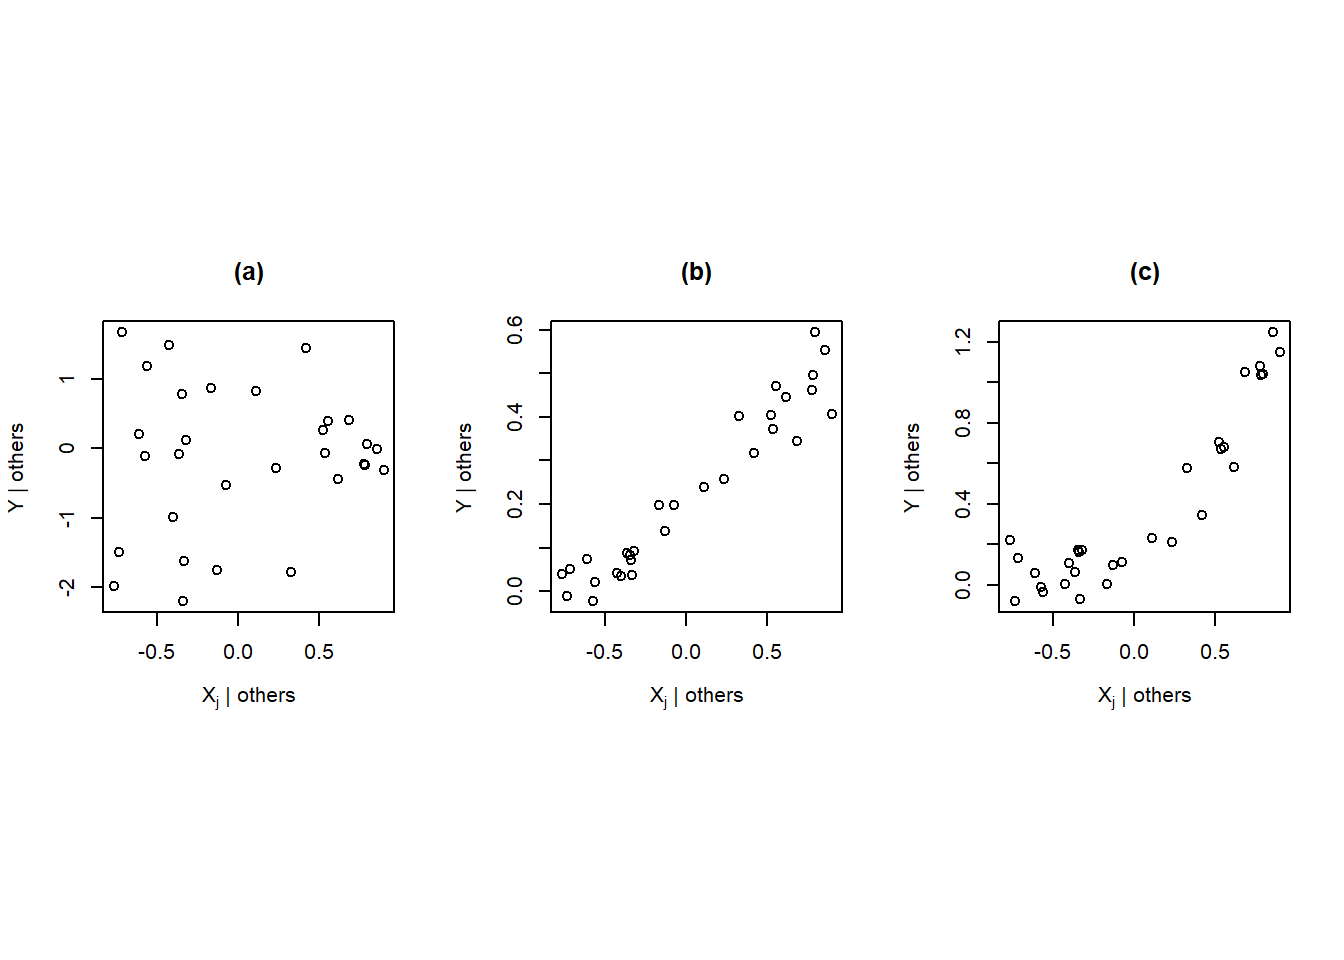
\includegraphics{A-Progessive-Introduction-to-Linear-Models_files/figure-latex/avplot-examples-1.pdf}
\caption{\label{fig:avplot-examples}Examples of added-variable plots}
\end{figure}

The \textbf{\texttt{car}} package (\protect\hyperlink{ref-R-car}{Fox, Weisberg, and Price 2022}) provides the \texttt{avPlot} and \texttt{avPlots}
functions for creating added-variable plots. The \texttt{avPlot} function will
produce an added-variable plot for a single regressor while the
\texttt{avPlots} function will produce added-variable plots for one or more
regressors.

The main arguments to the \texttt{avPlot} function are:

\begin{itemize}
\item
  \texttt{model}: the fitted \texttt{lm} (or \texttt{glm}) object.
\item
  \texttt{variable}: the regressor for which to create an added-variable
  plot.
\item
  \texttt{id}: a logical value indicating whether unusual observations should
  be identified. By default, the value is \texttt{TRUE}, which means the 2
  points with the largest residuals and the 2 points with the largest
  partial leverage are identified, though this can be customized.
\end{itemize}

The \texttt{avPlots} function replaces the \texttt{variable} argument with the \texttt{terms}
argument. The \texttt{terms} argument should be a one-sided formula to indicate
the regressors for which we want to construct added-variable plots (one
plot for each term). By default, an added-variable plot is created for
each regressor. Run \texttt{car::avPlot} in the Console for information about
about the arguments and details of the \texttt{avPlot} and \texttt{avPlots} functions.

We now create and interpret added-variable plots for the model
regressing \texttt{bill\_length\_mm} on \texttt{body\_mass\_g} and \texttt{flipper\_length\_mm},
which was previously assigned the name \texttt{mlmod}. We first load the
\textbf{\texttt{car}} package and then use the \texttt{avPlots} function to construct
added-variable plots for \texttt{body\_mass\_g} and \texttt{flipper\_length\_mm}. Figure
\ref{fig:avplots-mlmod} displays the added-variable plots for
\texttt{body\_mass\_g} and \texttt{flipper\_length\_mm}. The blue line is the simple
linear regression model that minimizes the RSS of the points. The
added-variable plot for \texttt{body\_mass\_g} exhibits a weak positive linear
relationship between the points. After using the \texttt{flipper\_length\_mm}
variable to explain the behavior of \texttt{bill\_length\_mm}, \texttt{body\_mass\_g}
likely has some additional explanatory power, but it doesn't explain a
lot of additional response variation. The added-variable plot for
\texttt{flipper\_length\_mm} exhibits a slightly stronger positive linear
relationship. The \texttt{flipper\_length\_mm} variable seems to have some
additional explanatory power when added to the model regressing
\texttt{bill\_length\_mm} on \texttt{body\_mass\_g}.

\begin{Shaded}
\begin{Highlighting}[]
\FunctionTok{library}\NormalTok{(car)}
\DocumentationTok{\#\# }
\DocumentationTok{\#\# Attaching package: \textquotesingle{}car\textquotesingle{}}
\DocumentationTok{\#\# The following object is masked from \textquotesingle{}package:dplyr\textquotesingle{}:}
\DocumentationTok{\#\# }
\DocumentationTok{\#\#     recode}
\DocumentationTok{\#\# The following object is masked from \textquotesingle{}package:purrr\textquotesingle{}:}
\DocumentationTok{\#\# }
\DocumentationTok{\#\#     some}
\CommentTok{\# create added{-}variable plots for all regressors in mlmod}
\FunctionTok{avPlots}\NormalTok{(mlmod)}
\end{Highlighting}
\end{Shaded}

\begin{figure}
\centering
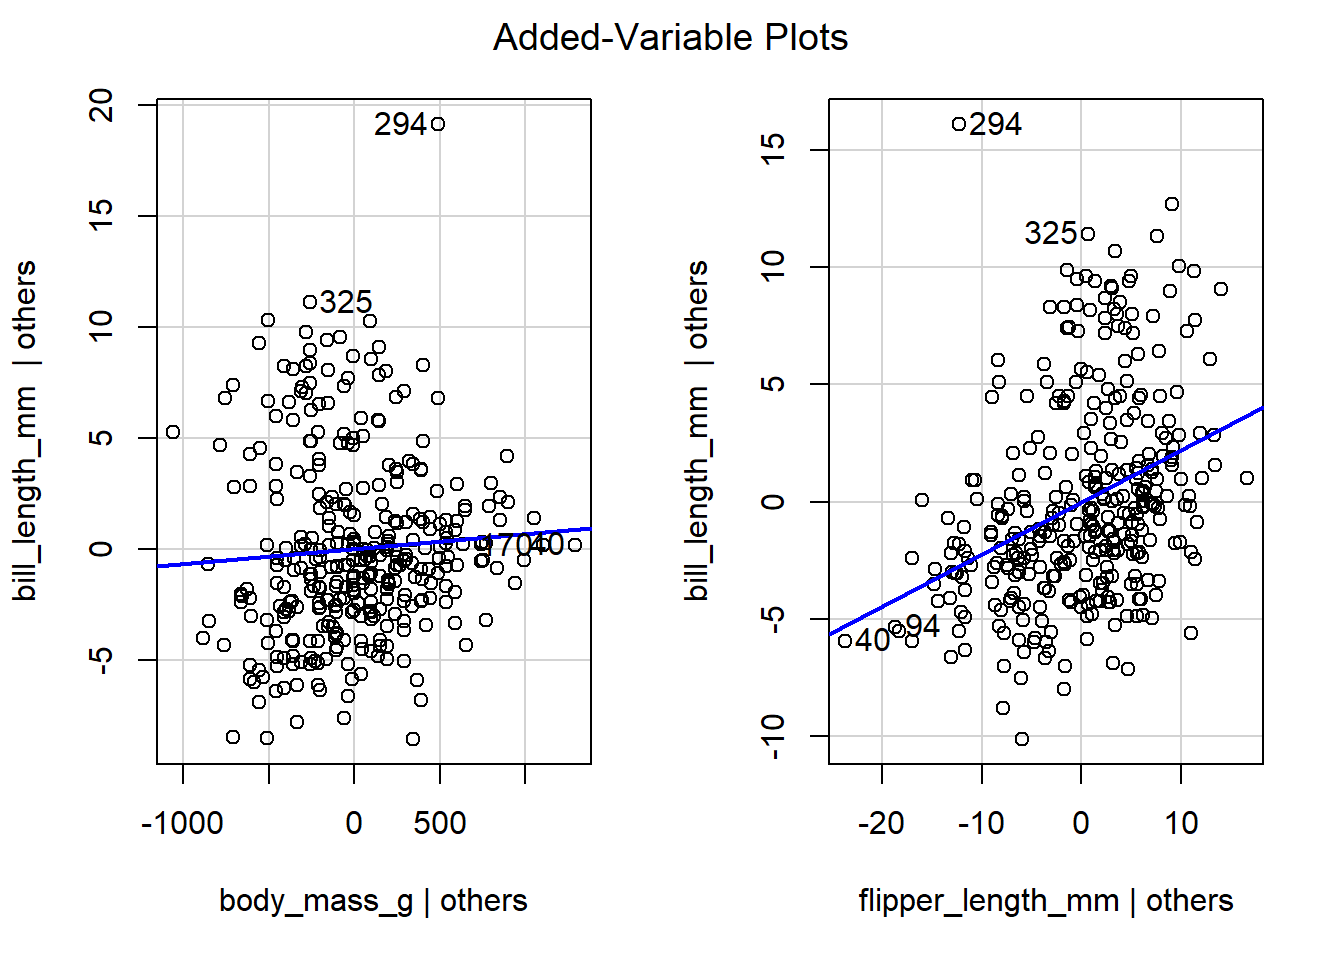
\includegraphics{A-Progessive-Introduction-to-Linear-Models_files/figure-latex/avplots-mlmod-1.pdf}
\caption{\label{fig:avplots-mlmod}The added-variable plots of all regressors for the model regressing \texttt{bill\_length\_mm} on \texttt{body\_mass\_g} and \texttt{flipper\_length\_mm}.}
\end{figure}

The added-variable plots of fitted models with categorical predictors
often show ``clusters'' of points related to the categorical predictors.
These clusters aren't anything to worry about unless the overall pattern
of the points is non-linear. We use the code below to create the
added-variable plots for all regressors in the parallel lines model
previously fit to the \texttt{penguins} data. The fitted model was \[
\begin{aligned}
&\hat{E}(\mathtt{bill\_length\_mm} \mid \mathtt{body\_mass\_g}, \mathtt{species})\\
&= 24.92 + 0.004 \mathtt{body\_mass\_g} + 9.92 D_C + 3.56 D_G,
\end{aligned}
\] where \(D_C\) and \(D_G\) are indicator variables for the Chinstrap and
Gentoo penguin species (Adelie penguins are the reference species).
Figure \ref{fig:avplots-lmodp} displays the added-variable plots for
the \texttt{body\_mass\_g} regressor and the indicator variables for Chinstrap
and Gentoo penguins. The added-variable plot for \texttt{body\_mass\_g} has a
moderately strong linear relationship, so adding \texttt{body\_mass\_g} to the
model regressing \texttt{bill\_length\_mm} on \texttt{species} seems to be beneficial.
The other two variable plots are show a linear relationship. Clustering
patterns are apparent in the added-variable plot for the Chinstrap
penguins indicator variable (\texttt{speciesChinstrap}) but not for the Gentoo
penguins indicator variable.

\begin{Shaded}
\begin{Highlighting}[]
\FunctionTok{avPlots}\NormalTok{(lmodp)}
\end{Highlighting}
\end{Shaded}

\begin{figure}
\centering
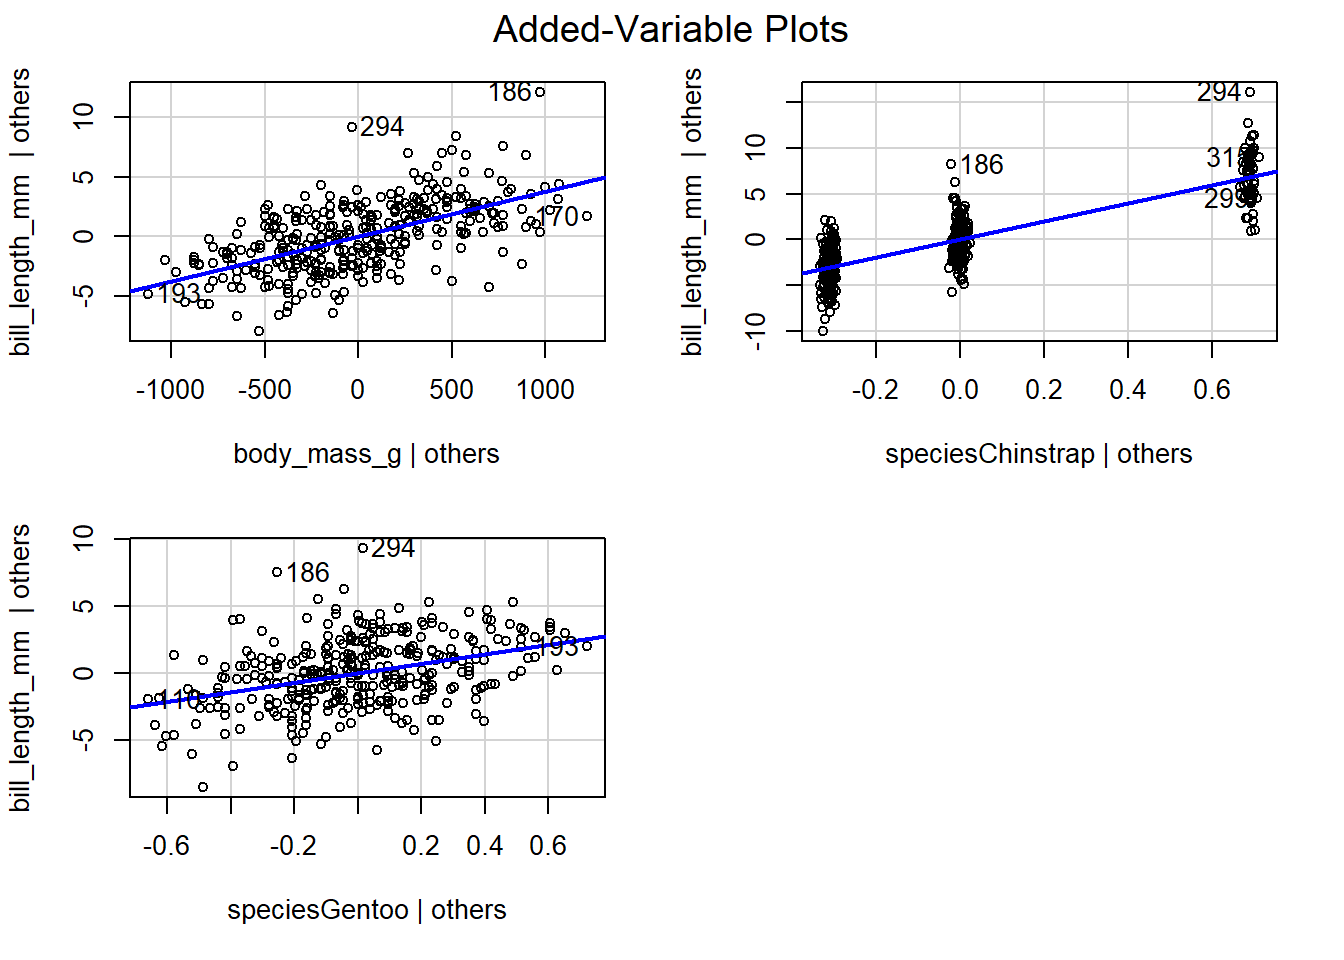
\includegraphics{A-Progessive-Introduction-to-Linear-Models_files/figure-latex/avplots-lmodp-1.pdf}
\caption{\label{fig:avplots-lmodp}The added-variable plots for all regressors in the parallel lines model fit to the \texttt{penguins} data.}
\end{figure}

A challenge in interpreting the added-variable plots of indicator
variable regressors is that it often doesn't make sense to talk about
the effect of adding a single regressor when all of the other
regressors are in the model. Specifically, we either add the categorical
\emph{predictor} to our regression model or we do not. When we add a
categorical predictor to our model, we simultaneously add \(K-1\)
indicator variables as regressors; we do not add the indicator variables
one-at-a-time. In general, we refer to regressors with this behavior as
``multiple degrees-of-freedom terms''. A categorical variable with 3 or
more levels is the most basic of multiple degrees-of-freedom term, but
we can also consider regressors related to the interaction between
two or more predictors, polynomial regressors, etc.

A \textbf{leverage plot} is an extension of the added-variable plot that
allows us to visualize the impact of multiple degrees-of-freedom terms.
Sall (\protect\hyperlink{ref-sall1990leverage}{1990}) originally proposed leverage plots to visualize
hypothesis tests of linear hypotheses. The interpretation of leverage
plots is similar to the interpretation of added-variable plots, though
we refer to ``predictors'' or ``terms'' instead regressors (which may be
combined into one plot). The \texttt{leveragePlot} and \texttt{leveragePlots}
functions in the \textbf{\texttt{car}} package produce single or multiple leverage
plots, respectively, with arguments similar to the \texttt{avPlot} and
\texttt{avPlots} functions.

We use the code below to create Figure \ref{fig:leverageplot-lmodp},
which displays leverage plots for the \texttt{body\_mass\_g} and \texttt{species}
predictors of the parallel lines model previously fit to the \texttt{penguins}
data. The leverage plot for \texttt{body\_mass\_g} has a moderate linear
relationship, so we expect \texttt{body\_mass\_g} to have moderate value in
explaining the behavior of \texttt{bill\_length\_mm} after accounting for
\texttt{species}. Similarly, the points in the leverage plot for \texttt{species} have
a moderately strong linear relationship, so we expect \texttt{species} to have
moderate value in explaining the behavior of \texttt{bill\_length\_mm} after
accounting for \texttt{body\_mass\_g}.

\begin{Shaded}
\begin{Highlighting}[]
\FunctionTok{leveragePlots}\NormalTok{(lmodp)}
\end{Highlighting}
\end{Shaded}

\begin{figure}
\centering
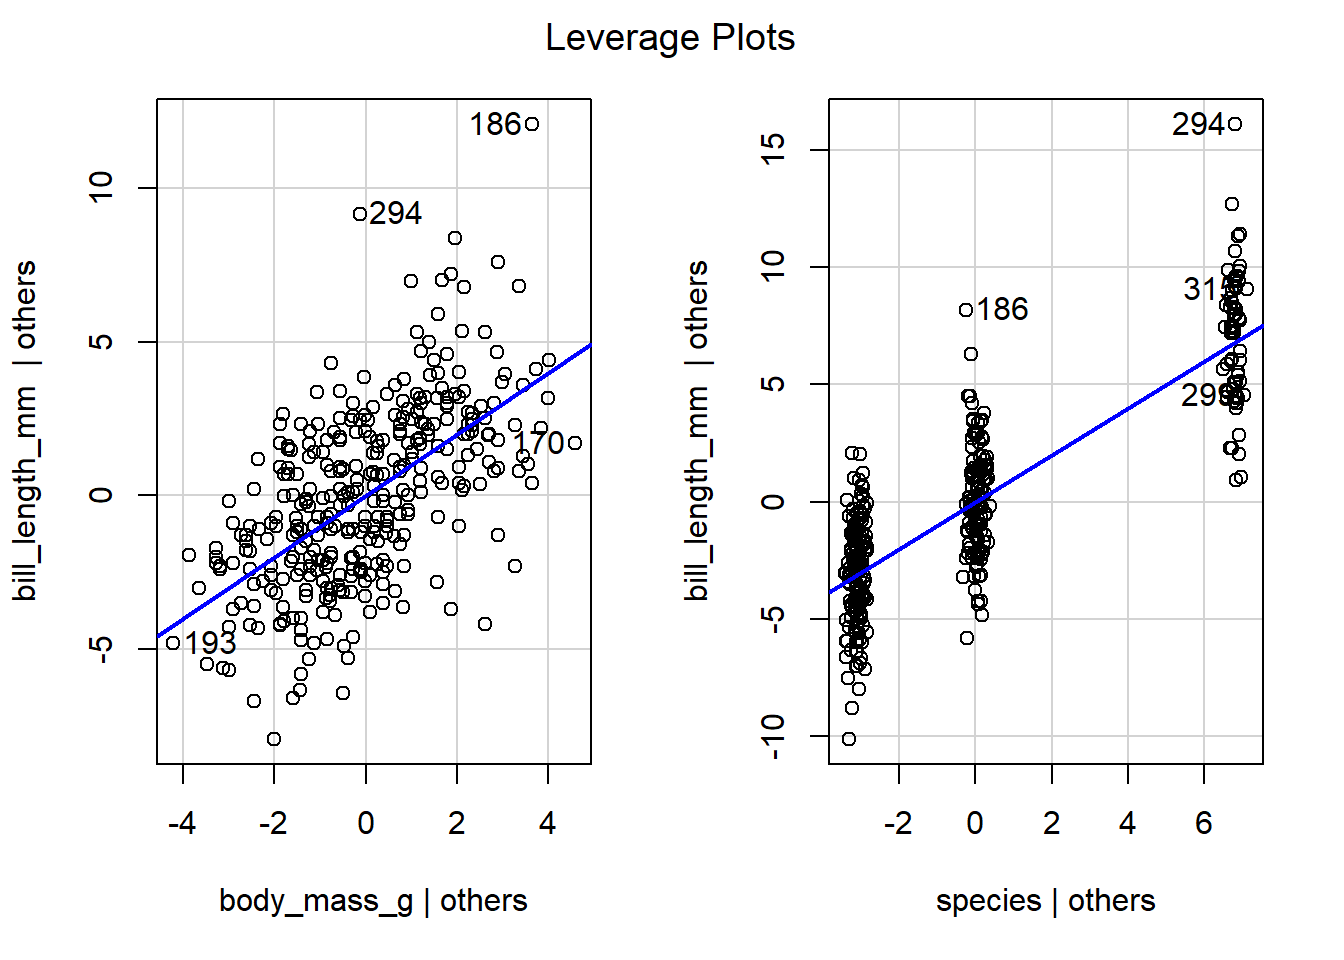
\includegraphics{A-Progessive-Introduction-to-Linear-Models_files/figure-latex/leverageplot-lmodp-1.pdf}
\caption{\label{fig:leverageplot-lmodp}Leverage plots for the predictors in the parallel lines model fit to the \texttt{penguins} data.}
\end{figure}

We next examine the leverage plot for the separate lines model fit to
the \texttt{penguins} data. The fitted separate lines model is\[
\begin{aligned}
&\hat{E}(\mathtt{bill\_length\_mm} \mid \mathtt{body\_mass\_g}, \mathtt{species}) \\
&= 26.99 + 0.003 \mathtt{body\_mass\_g} + 5.18 D_C - 0.25 D_G \\
&\quad + 0.001 D_C \mathtt{body\_mass\_g} + 0.0009 D_G \mathtt{body\_mass\_g},
\end{aligned}
\]which has 6 estimated coefficients. However, the fitted model has only
3 non-intercept terms. Recall the formula we fit for the separate lines
model:

\begin{Shaded}
\begin{Highlighting}[]
\CommentTok{\# function call for separate lines model}
\FunctionTok{lm}\NormalTok{(}\AttributeTok{formula =}\NormalTok{ bill\_length\_mm }\SpecialCharTok{\textasciitilde{}}\NormalTok{ body\_mass\_g }\SpecialCharTok{+}\NormalTok{ species }\SpecialCharTok{+}\NormalTok{ body\_mass\_g}\SpecialCharTok{:}\NormalTok{species,}
   \AttributeTok{data =}\NormalTok{ penguins)}
\end{Highlighting}
\end{Shaded}

Thus, we have terms for \texttt{body\_mass\_g}, \texttt{species}, and the interaction
term \texttt{body\_mass\_g:species}.

We use the code below to create the leverage plots shown in Figure
\ref{fig:leverageplot-lmods}. The leverage plot for \texttt{body\_mass\_g} has a
moderate linear relationship, so we expect \texttt{body\_mass\_g} to have
moderate additional value in explaining the behavior of \texttt{bill\_length\_mm}
after accounting for \texttt{species} and the interaction term
\texttt{body\_mass\_g:species}. It is unlikely we would include the
\texttt{body\_mass\_g:species} term in our model prior to including \texttt{body\_mass\_g}
, so philosophically, this plot provides little useful information.
Similarly, interpreting the leverage plot for \texttt{species} has limited
utility because the leverage plot includes the influence of the
interaction term \texttt{body\_mass\_g:species}. We are unlikely to fit a model
that includes the interaction term without also including the \texttt{species}
term directly. Instead it makes more sense to judge the utility of
adding \texttt{species} to the model regressing \texttt{bill\_length\_mm} on
\texttt{body\_mass\_g} alone, which we already considered in Figure
\ref{fig:leverageplot-lmodp}. Examining the leverage plot for the
interaction term \texttt{body\_mass\_g:species} , we see the points have only a
weak linear relationship. Thus, we expect limited utility in adding the
interaction term \texttt{body\_mass\_g:species} to the parallel lines regression
model that regresses \texttt{bill\_length\_mm} on \texttt{body\_mass\_g} and \texttt{species}.

\begin{Shaded}
\begin{Highlighting}[]
\FunctionTok{leveragePlots}\NormalTok{(lmods)}
\end{Highlighting}
\end{Shaded}

\begin{figure}
\centering
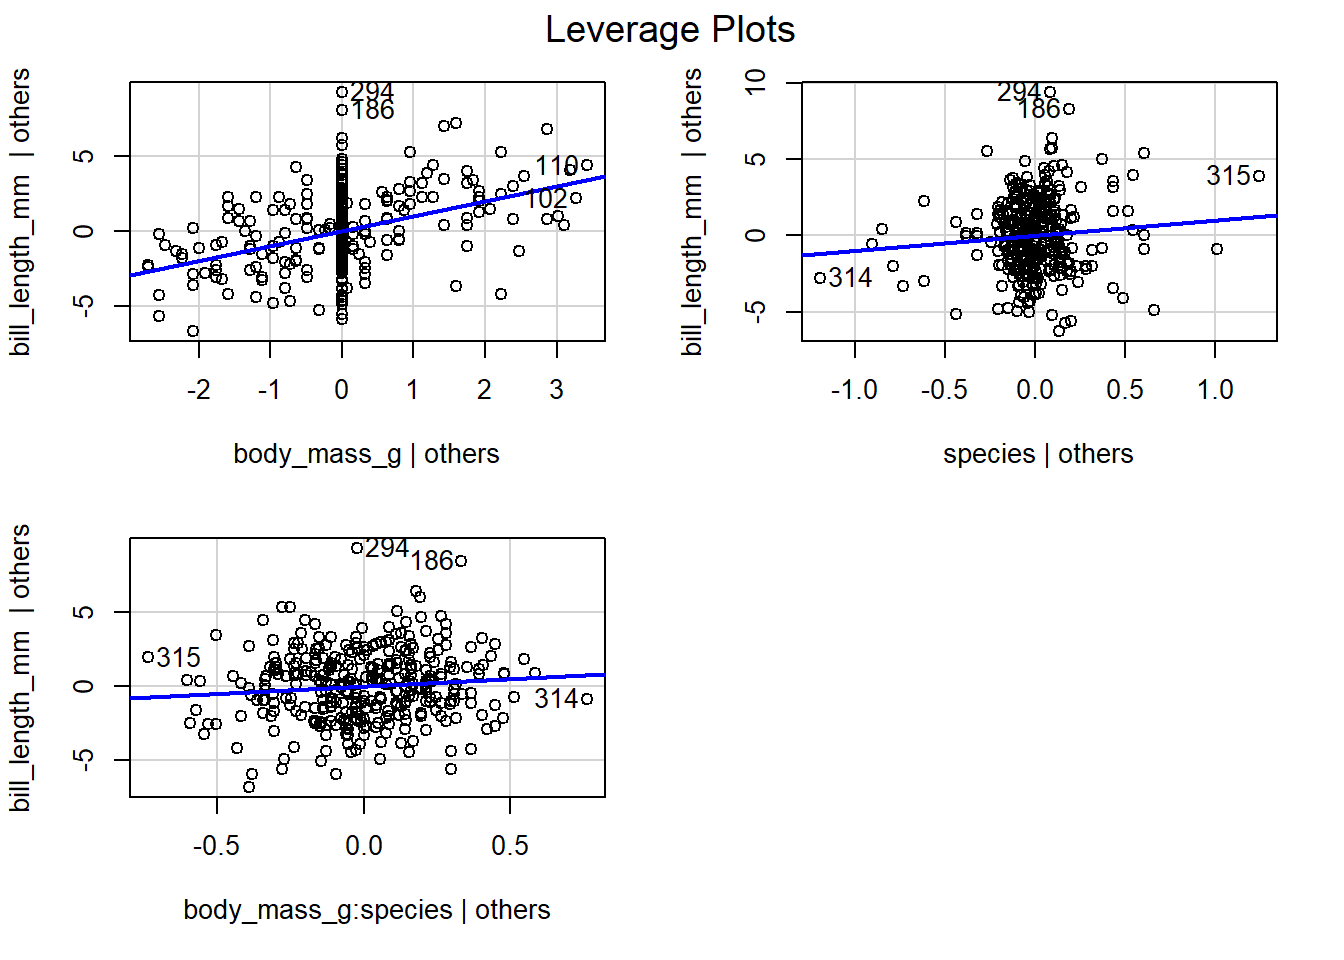
\includegraphics{A-Progessive-Introduction-to-Linear-Models_files/figure-latex/leverageplot-lmods-1.pdf}
\caption{\label{fig:leverageplot-lmods}Leverage plots for the terms in the separate lines model fit to the \texttt{penguins} data.}
\end{figure}

\hypertarget{going-deeper-1}{%
\section{Going deeper}\label{going-deeper-1}}

\hypertarget{orthogonality}{%
\subsection{Orthogonality}\label{orthogonality}}

Let \[\mathbf{X}_{[j]}=[x_{1,j},\ldots,x_{n,j}]\] denote the \(n\times 1\)
column vector of observed values for column \(j\) of \(\mathbf{X}\). (We can't use the
notation \(\mathbf{x}_j\) because that is the \(p\times 1\) vector of
regressor values for the \(j\)th observation).

Regressors
\(\mathbf{X}_{[j]}\) and \(\mathbf{X}_{[k]}\) are \textbf{orthogonal} if
\(\mathbf{X}_{[j]}^T \mathbf{X}_{[k]}=0\).

Let \(\boldsymbol{1}_{n\times1}\) denote an \(n\times 1\) column vector of
1s. The definition of orthogonal vectors above implies that
\(\mathbf{X}_{[j]}\) is orthogonal to \(\boldsymbol{1}_{n\times1}\) if \[
\mathbf{X}_{[j]}^T \boldsymbol{1}_{n\times1} = \sum_{i=1}^n x_{i,j} = 0,\]
i.e., if the values in \(\mathbf{X}_{[j]}\) sum to zero.

Let \(\bar{x}_j = \frac{1}{n}\sum_{i=1}^n x_{i,j}\) denote the sample mean
of \(\mathbf{X}_{[j]}\) and
\(\bar{\mathbf{x}}_j = \bar{x}_j \boldsymbol{1}_{n\times 1}\) denote the
column vector that repeats \(\bar{x}_j\) \(n\) times.

\textbf{Centering} \(\mathbf{X}_{[j]}\) involves subtracting the sample mean of
\(\mathbf{X}_{[j]}\) from \(\mathbf{X}_{[j]}\), i.e.,
\(\mathbf{X}_{[j]} - \bar{\mathbf{x}}_j\).

Regressors \(\mathbf{X}_{[j]}\) and \(\mathbf{X}_{[k]}\) are
\textbf{uncorrelated} if they are orthogonal after being centered, i.e., if
\[
(\mathbf{X}_{[j]} - \bar{\mathbf{x}}_j)^T (\mathbf{X}_{[k]} - \bar{\mathbf{x}}_k)=0.
\] Note that the sample covariance between vectors \(\mathbf{X}_{[j]}\)
and \(\mathbf{X}_{[k]}\) is \[
\begin{aligned}
\widehat{\mathrm{cov}}(\mathbf{X}_{[j]}, \mathbf{X}_{[k]}) &= \frac{1}{n-1}\sum_{i=1}^n (x_{i,j} - \bar{x}_j)(x_{i,k} - \bar{x}_k) \\
 &= \frac{1}{n-1}(\mathbf{X}_{[j]} - \bar{\mathbf{x}}_j)^T (\mathbf{X}_{[k]} - \bar{\mathbf{x}}_k).
\end{aligned}
\]Thus, two centered regressors are orthogonal if their covariance is
zero.

It is a desirable to have orthogonal regressors in our fitted model
because they simplify estimating the relationship between the regressors
and the response. Specifically:

\emph{If a regressor is orthogonal to all other regressors (and the column of
1s) in a model, adding or removing the orthogonal regressor from our
model will not impact the estimated regression coefficients of the other
regressors.}

Since most linear regression models include an intercept, we should
assess whether our regressors are orthogonal to other regressors and the
column of 1s.

We consider a simple example with \(n=5\) observations to demonstrate how orthogonality of regressors impacts the estimated regression coefficients.

In the code below:

\begin{itemize}
\tightlist
\item
  \texttt{y} is a vector of response values.
\item
  \texttt{X1} is a column vector of regressor values.
\item
  \texttt{X2} is a column vector of regressor values chosen to be orthogonal to \texttt{X1}.
\end{itemize}

\begin{Shaded}
\begin{Highlighting}[]
\NormalTok{y }\OtherTok{\textless{}{-}} \FunctionTok{c}\NormalTok{(}\DecValTok{1}\NormalTok{, }\DecValTok{4}\NormalTok{, }\DecValTok{6}\NormalTok{, }\DecValTok{8}\NormalTok{, }\DecValTok{9}\NormalTok{)       }\CommentTok{\# create an arbitrary response vector}
\NormalTok{X1 }\OtherTok{\textless{}{-}} \FunctionTok{c}\NormalTok{(}\DecValTok{7}\NormalTok{, }\DecValTok{5}\NormalTok{, }\DecValTok{5}\NormalTok{, }\DecValTok{7}\NormalTok{, }\DecValTok{7}\NormalTok{)      }\CommentTok{\# create regressor 1}
\NormalTok{X2 }\OtherTok{\textless{}{-}} \FunctionTok{c}\NormalTok{(}\SpecialCharTok{{-}}\DecValTok{1}\NormalTok{, }\DecValTok{2}\NormalTok{, }\SpecialCharTok{{-}}\DecValTok{3}\NormalTok{, }\DecValTok{1}\NormalTok{, }\DecValTok{5}\SpecialCharTok{/}\DecValTok{7}\NormalTok{)  }\CommentTok{\# create regressor 2 to be orthogonal to X1}
\end{Highlighting}
\end{Shaded}

Note that the \texttt{crossprod} function computes the cross product of two vectors or matrices, so that \texttt{crossprod(A,\ B)} computes \(\mathbf{A}^T B\), where the vectors or matrices must have the correct dimension for the multiplication to be performed.

The regressor vectors \texttt{X1} and \texttt{X2} are orthogonal since their cross product \(\mathbf{X}_{[1]}^T \mathbf{X}_{[2]}\) (in R, \texttt{crossprod(X1,\ X2)}) equals zero, as shown in the code below.

\begin{Shaded}
\begin{Highlighting}[]
\CommentTok{\# cross product is zero, so X1 and X2 are orthogonal}
\FunctionTok{crossprod}\NormalTok{(X1, X2)}
\DocumentationTok{\#\#      [,1]}
\DocumentationTok{\#\# [1,]    0}
\end{Highlighting}
\end{Shaded}

In the code below, we regress \texttt{y} on \texttt{X1} without an intercept (\texttt{lmod1}). The estimated coefficient for \texttt{X1} is \(\hat{\beta}_1=0.893\).

\begin{Shaded}
\begin{Highlighting}[]
\CommentTok{\# y regressed on X1 without an intercept}
\NormalTok{lmod1 }\OtherTok{\textless{}{-}} \FunctionTok{lm}\NormalTok{(y }\SpecialCharTok{\textasciitilde{}}\NormalTok{ X1 }\SpecialCharTok{{-}} \DecValTok{1}\NormalTok{)}
\FunctionTok{coef}\NormalTok{(lmod1)}
\DocumentationTok{\#\#       X1 }
\DocumentationTok{\#\# 0.893401}
\end{Highlighting}
\end{Shaded}

Next, we then regress \texttt{y} on \texttt{X1} and \texttt{X2} without an intercept (\texttt{lmod2}). The estimated coefficients for \texttt{X1} and \texttt{X2} are \(\hat{\beta}_1=0.893\) and \(\hat{\beta}_2=0.221\), respectively. Because \texttt{X1} and \texttt{X2} are orthogonal (and because there are no other regressors to consider in the model), the estimated coefficient for \texttt{X1} stays the
same in both models.

\begin{Shaded}
\begin{Highlighting}[]
\CommentTok{\# y regressed on X1 and X2 without an intercept}
\NormalTok{lmod2 }\OtherTok{\textless{}{-}} \FunctionTok{lm}\NormalTok{(y }\SpecialCharTok{\textasciitilde{}}\NormalTok{ X1 }\SpecialCharTok{+}\NormalTok{ X2 }\SpecialCharTok{{-}} \DecValTok{1}\NormalTok{)}
\FunctionTok{coef}\NormalTok{(lmod2)}
\DocumentationTok{\#\#        X1        X2 }
\DocumentationTok{\#\# 0.8934010 0.2210526}
\end{Highlighting}
\end{Shaded}

The previous models (\texttt{lmod1} and \texttt{lmod2}) neglect an important characteristic of a typical linear model: we usually include an intercept coefficient (a columns of 1s as a regressor) in our model. If the regressors are not orthogonal to the column of 1s in our \(\mathbf{X}\) matrix, then the coefficients for the other regressors in
the model will change when the regressors are added or removed from the model because they are not orthogonal to the column of 1s.

We create a vector \texttt{ones} that is simply a column of 1s.

\begin{Shaded}
\begin{Highlighting}[]
\NormalTok{ones }\OtherTok{\textless{}{-}} \FunctionTok{rep}\NormalTok{(}\DecValTok{1}\NormalTok{, }\DecValTok{5}\NormalTok{)   }\CommentTok{\# column of 1s}
\end{Highlighting}
\end{Shaded}

Neither \texttt{X1} nor \texttt{X2} is orthogonal with the column of ones. We compute the cross product between \texttt{ones} and the two regressors \texttt{X1} and \texttt{X2}. Since the cross products are not zero, \texttt{X1} and \texttt{X2} are not orthogonal to the
column of ones.

\begin{Shaded}
\begin{Highlighting}[]
\FunctionTok{crossprod}\NormalTok{(ones, X1) }\CommentTok{\# not zero, so not orthogonal}
\DocumentationTok{\#\#      [,1]}
\DocumentationTok{\#\# [1,]   31}
\FunctionTok{crossprod}\NormalTok{(ones, X2) }\CommentTok{\# not zero, so not orthogonal}
\DocumentationTok{\#\#            [,1]}
\DocumentationTok{\#\# [1,] {-}0.2857143}
\end{Highlighting}
\end{Shaded}

We create \texttt{lmod3} by adding adding a column of ones to \texttt{lmod2} (i.e.,
we include the intercept in the model). The the coefficients for both
\texttt{X1} and \texttt{X2} change when going from \texttt{lmod2} to \texttt{lmod3} because these
regressors are not orthogonal to the column of 1s. Comparing the
coefficients \texttt{lmod2} above and \texttt{lmod3}, \(\hat{\beta}_1\) changes from
\(0.893\) to \(0.397\) and \(\hat{\beta}_2\) changes from \(0.221\) to \(0.279\).

\begin{Shaded}
\begin{Highlighting}[]
\FunctionTok{coef}\NormalTok{(lmod2) }\CommentTok{\# coefficients for lmod2}
\DocumentationTok{\#\#        X1        X2 }
\DocumentationTok{\#\# 0.8934010 0.2210526}
\CommentTok{\# y regressed on X1 and X2 with an intercept}
\NormalTok{lmod3 }\OtherTok{\textless{}{-}} \FunctionTok{lm}\NormalTok{(y }\SpecialCharTok{\textasciitilde{}}\NormalTok{ X1 }\SpecialCharTok{+}\NormalTok{ X2)}
\FunctionTok{coef}\NormalTok{(lmod3) }\CommentTok{\# coefficients for lmod3}
\DocumentationTok{\#\# (Intercept)          X1          X2 }
\DocumentationTok{\#\#   3.1547101   0.3969746   0.2791657}
\end{Highlighting}
\end{Shaded}

For orthogonality of our regressors to be most impactful, the model's
regressors should be orthogonal to each other and the column of 1s. In
that context, adding or removing any of the regressors doesn't impact
the estimated coefficients of the other regressors. In the code below,
we define centered regressors \texttt{X3} and \texttt{X4} to be uncorrelated, i.e.,
\texttt{X3} and \texttt{X4} have sample mean zero and are orthogonal to each other.

\begin{Shaded}
\begin{Highlighting}[]
\NormalTok{X3 }\OtherTok{\textless{}{-}}  \FunctionTok{c}\NormalTok{(}\DecValTok{0}\NormalTok{, }\SpecialCharTok{{-}}\DecValTok{1}\NormalTok{, }\DecValTok{1}\NormalTok{, }\DecValTok{0}\NormalTok{, }\DecValTok{0}\NormalTok{) }\CommentTok{\# sample mean is zero}
\NormalTok{X4 }\OtherTok{\textless{}{-}} \FunctionTok{c}\NormalTok{(}\DecValTok{0}\NormalTok{, }\DecValTok{0}\NormalTok{, }\DecValTok{0}\NormalTok{, }\DecValTok{1}\NormalTok{, }\SpecialCharTok{{-}}\DecValTok{1}\NormalTok{)  }\CommentTok{\# sample mean is zero}
\FunctionTok{cov}\NormalTok{(X3, X4)              }\CommentTok{\# 0, so X3 and X4 are uncorrelated and orthogonal}
\DocumentationTok{\#\# [1] 0}
\end{Highlighting}
\end{Shaded}

If we fit linear regression models with any combination of \texttt{ones}, \texttt{X3},
or \texttt{X4} as regressors, the associated regression coefficients will not
change. To demonstrate this, we consider all possible combinations of
the three variables in the models below. We do not run the code to save
space, but we summarize the results below.

\begin{Shaded}
\begin{Highlighting}[]
\FunctionTok{coef}\NormalTok{(}\FunctionTok{lm}\NormalTok{(y }\SpecialCharTok{\textasciitilde{}} \DecValTok{1}\NormalTok{))           }\CommentTok{\# only column of 1s}
\FunctionTok{coef}\NormalTok{(}\FunctionTok{lm}\NormalTok{(y }\SpecialCharTok{\textasciitilde{}}\NormalTok{ X3 }\SpecialCharTok{{-}} \DecValTok{1}\NormalTok{))      }\CommentTok{\# only X3}
\FunctionTok{coef}\NormalTok{(}\FunctionTok{lm}\NormalTok{(y }\SpecialCharTok{\textasciitilde{}}\NormalTok{ X4 }\SpecialCharTok{{-}} \DecValTok{1}\NormalTok{))      }\CommentTok{\# only X4}
\FunctionTok{coef}\NormalTok{(}\FunctionTok{lm}\NormalTok{(y }\SpecialCharTok{\textasciitilde{}}\NormalTok{ X3))          }\CommentTok{\# 1s and X3}
\FunctionTok{coef}\NormalTok{(}\FunctionTok{lm}\NormalTok{(y }\SpecialCharTok{\textasciitilde{}}\NormalTok{ X4))          }\CommentTok{\# 1s and X4}
\FunctionTok{coef}\NormalTok{(}\FunctionTok{lm}\NormalTok{(y }\SpecialCharTok{\textasciitilde{}}\NormalTok{ X3 }\SpecialCharTok{+}\NormalTok{ X4 }\SpecialCharTok{{-}} \DecValTok{1}\NormalTok{)) }\CommentTok{\# X3 and X4}
\FunctionTok{coef}\NormalTok{(}\FunctionTok{lm}\NormalTok{(y }\SpecialCharTok{\textasciitilde{}}\NormalTok{ X3 }\SpecialCharTok{+}\NormalTok{ X4))     }\CommentTok{\# 1s, X3, and X4}
\end{Highlighting}
\end{Shaded}

We simply note that in each of the previous models, because all of the
regressors (and the column of 1s) are orthogonal to each other, adding
or removing any regressor doesn't impact the estimated coefficients for
the other regressors in the model. Thus, the estimated coefficients were
\(\hat{\beta}_{0}=5.6\), \(\hat{\beta}_{3}=1.0\), \(\hat{\beta}_{4}=-0.5\)
when the relevant regressor was included in the model.

The easiest way to determine which vectors are orthogonal to each other
and the intercept is to compute the cross product of the \(\mathbf{X}\)
matrix for the largest set of regressors we are considering. Consider
the matrix of cross products for the columns of 1s, \texttt{X1}, \texttt{X2}, \texttt{X3}, and
\texttt{X4}.

\begin{Shaded}
\begin{Highlighting}[]
\FunctionTok{crossprod}\NormalTok{(}\FunctionTok{model.matrix}\NormalTok{(}\SpecialCharTok{\textasciitilde{}}\NormalTok{ X1 }\SpecialCharTok{+}\NormalTok{ X2 }\SpecialCharTok{+}\NormalTok{ X3 }\SpecialCharTok{+}\NormalTok{ X4))}
\DocumentationTok{\#\#             (Intercept)  X1         X2 X3        X4}
\DocumentationTok{\#\# (Intercept)   5.0000000  31 {-}0.2857143  0 0.0000000}
\DocumentationTok{\#\# X1           31.0000000 197  0.0000000  0 0.0000000}
\DocumentationTok{\#\# X2           {-}0.2857143   0 15.5102041 {-}5 0.2857143}
\DocumentationTok{\#\# X3            0.0000000   0 {-}5.0000000  2 0.0000000}
\DocumentationTok{\#\# X4            0.0000000   0  0.2857143  0 2.0000000}
\end{Highlighting}
\end{Shaded}

Consider the sequence of models below.

\begin{Shaded}
\begin{Highlighting}[]
\FunctionTok{coef}\NormalTok{(}\FunctionTok{lm}\NormalTok{(y }\SpecialCharTok{\textasciitilde{}} \DecValTok{1}\NormalTok{))}
\DocumentationTok{\#\# (Intercept) }
\DocumentationTok{\#\#         5.6}
\end{Highlighting}
\end{Shaded}

The model with only an intercept has an estimated coefficient of
\(\hat{\beta}_{0}=5.6\). If we add the \texttt{X1} to the model with an
intercept, then the intercept coefficient changes because the column of 1s isn't orthogonal to \texttt{X1}.

\begin{Shaded}
\begin{Highlighting}[]
\NormalTok{lmod4 }\OtherTok{\textless{}{-}} \FunctionTok{lm}\NormalTok{(y }\SpecialCharTok{\textasciitilde{}}\NormalTok{ X1) }\CommentTok{\# model with 1s and X1}
\FunctionTok{coef}\NormalTok{(lmod4)}
\DocumentationTok{\#\# (Intercept)          X1 }
\DocumentationTok{\#\#         2.5         0.5}
\end{Highlighting}
\end{Shaded}

If we add \texttt{X2} to \texttt{lmod4}, we might think that only \(\hat{\beta}_{0}\)
will change because \texttt{X1} and \texttt{X2} are orthogonal to each other. However,
because \texttt{X2} is not orthogonal to all of the other regressors in the
model (\texttt{X1} and the column of 1s), both \(\hat{\beta}_{0}\) and
\(\hat{\beta}_1\) will change. The easiest way to realize this is to look
at \texttt{lmod2} above with only \texttt{X1} and \texttt{X2}. When we add the column of 1s
to \texttt{lmod2}, both \(\hat{\beta}_1\) and \(\hat{\beta}_2\) will change because
neither regressor is orthogonal to the column of 1s needed to include
the intercept term.

\begin{Shaded}
\begin{Highlighting}[]
\FunctionTok{coef}\NormalTok{(}\FunctionTok{lm}\NormalTok{(y }\SpecialCharTok{\textasciitilde{}}\NormalTok{ X1 }\SpecialCharTok{+}\NormalTok{ X2))}
\DocumentationTok{\#\# (Intercept)          X1          X2 }
\DocumentationTok{\#\#   3.1547101   0.3969746   0.2791657}
\end{Highlighting}
\end{Shaded}

However, note that \texttt{X3} is orthogonal to the column of 1s and \texttt{X1}.
Thus, if we add \texttt{X3} to \texttt{lmod4}, which includes both a column of 1s and
\texttt{X1}, \texttt{X3} will not change the estimated coefficients for the intercept
or \texttt{X1}.

\begin{Shaded}
\begin{Highlighting}[]
\FunctionTok{coef}\NormalTok{(}\FunctionTok{lm}\NormalTok{(y }\SpecialCharTok{\textasciitilde{}}\NormalTok{ X1 }\SpecialCharTok{+}\NormalTok{ X3))}
\DocumentationTok{\#\# (Intercept)          X1          X3 }
\DocumentationTok{\#\#         2.5         0.5         1.0}
\end{Highlighting}
\end{Shaded}

Additionally, since \texttt{X4} is orthogonal to the column of 1s, \texttt{X1}, and
\texttt{X3}, adding \texttt{X4} to the previous model will not change the estimated
coefficients for any of the other variables already in the model.

\begin{Shaded}
\begin{Highlighting}[]
\FunctionTok{coef}\NormalTok{(}\FunctionTok{lm}\NormalTok{(y }\SpecialCharTok{\textasciitilde{}}\NormalTok{ X1 }\SpecialCharTok{+}\NormalTok{ X3 }\SpecialCharTok{+}\NormalTok{ X4))}
\DocumentationTok{\#\# (Intercept)          X1          X3          X4 }
\DocumentationTok{\#\#         2.5         0.5         1.0        {-}0.5}
\end{Highlighting}
\end{Shaded}

Lastly, if we can partition our \(\mathbf{X}\) matrix such that
\(\mathbf{X}^T \mathbf{X}\) is a block diagonal matrix, then none of the
blocks of variables will affect the estimated coefficients of the other
variables.

Define a new regressor \texttt{X5} below.

\begin{Shaded}
\begin{Highlighting}[]
\NormalTok{X5 }\OtherTok{\textless{}{-}} \FunctionTok{c}\NormalTok{(}\DecValTok{1}\NormalTok{, }\DecValTok{0}\NormalTok{, }\DecValTok{0}\NormalTok{, }\SpecialCharTok{{-}}\DecValTok{1}\NormalTok{, }\DecValTok{0}\NormalTok{) }\CommentTok{\# orthogonal to ones, X1, not X4}
\end{Highlighting}
\end{Shaded}

\texttt{X5} is orthogonal to the column of
1s and \texttt{X1}, but not \texttt{X4}, as evidenced in the code below.

\begin{Shaded}
\begin{Highlighting}[]
\CommentTok{\# note block of 0s}
\FunctionTok{crossprod}\NormalTok{(}\FunctionTok{cbind}\NormalTok{(ones, X1, X4, X5))}
\DocumentationTok{\#\#      ones  X1 X4 X5}
\DocumentationTok{\#\# ones    5  31  0  0}
\DocumentationTok{\#\# X1     31 197  0  0}
\DocumentationTok{\#\# X4      0   0  2 {-}1}
\DocumentationTok{\#\# X5      0   0 {-}1  2}
\end{Highlighting}
\end{Shaded}

Note the block of zeros in the lower left and upper right corners of the
cross product matrix above. The block containing \texttt{ones} and \texttt{X1} is
orthogonal to the block containing \texttt{X4} and \texttt{X5}. This means that if we
fit the model with only the column of 1s and \texttt{X1}, the model only with
\texttt{X4} and \texttt{X5}, and then fit the model with the column of 1s, \texttt{X1}, \texttt{X4},
and \texttt{X5}, then the coefficients \(\hat{\beta}_{0}\) and \(\hat{\beta}_{1}\)
are not impacted when \texttt{X4} and \texttt{X5} are added to the model. Similarly,
\(\hat{\beta}_{4}\) and \(\hat{\beta}_{5}\) are not impacted when the column
of 1s and \texttt{X1} are added to the model with \texttt{X4} and \texttt{X5}. See the output below.

\begin{Shaded}
\begin{Highlighting}[]
\FunctionTok{lm}\NormalTok{(y }\SpecialCharTok{\textasciitilde{}}\NormalTok{ X1)           }\CommentTok{\# model with 1s and X1}
\DocumentationTok{\#\# }
\DocumentationTok{\#\# Call:}
\DocumentationTok{\#\# lm(formula = y \textasciitilde{} X1)}
\DocumentationTok{\#\# }
\DocumentationTok{\#\# Coefficients:}
\DocumentationTok{\#\# (Intercept)           X1  }
\DocumentationTok{\#\#         2.5          0.5}
\FunctionTok{lm}\NormalTok{(y }\SpecialCharTok{\textasciitilde{}}\NormalTok{ X4 }\SpecialCharTok{+}\NormalTok{ X5 }\SpecialCharTok{{-}} \DecValTok{1}\NormalTok{)  }\CommentTok{\# model with X4 and X5 only}
\DocumentationTok{\#\# }
\DocumentationTok{\#\# Call:}
\DocumentationTok{\#\# lm(formula = y \textasciitilde{} X4 + X5 {-} 1)}
\DocumentationTok{\#\# }
\DocumentationTok{\#\# Coefficients:}
\DocumentationTok{\#\# X4  X5  }
\DocumentationTok{\#\# {-}3  {-}5}
\FunctionTok{lm}\NormalTok{(y }\SpecialCharTok{\textasciitilde{}}\NormalTok{ X1 }\SpecialCharTok{+}\NormalTok{ X4 }\SpecialCharTok{+}\NormalTok{ X5) }\CommentTok{\# model with 1s, X1, X4, X5}
\DocumentationTok{\#\# }
\DocumentationTok{\#\# Call:}
\DocumentationTok{\#\# lm(formula = y \textasciitilde{} X1 + X4 + X5)}
\DocumentationTok{\#\# }
\DocumentationTok{\#\# Coefficients:}
\DocumentationTok{\#\# (Intercept)           X1           X4           X5  }
\DocumentationTok{\#\#         2.5          0.5         {-}3.0         {-}5.0}
\end{Highlighting}
\end{Shaded}

\hypertarget{linear-model-theory}{%
\chapter{Basic theoretical results for linear models}\label{linear-model-theory}}

In this chapter we discuss many basic theoretical results for linear models. The results are not interesting by themselves, but they are foundational for the inferential results discussed in Chapter \ref{inference}. Appendices \ref{overview-of-matrix-facts} and \ref{prob-review} provide an overview of properties related to matrices and random vectors that are needed for the derivations below.

We assume the responses can be modeled as
\[
Y_i=\beta_0+\beta_1 x_{i,1} +\ldots + \beta_{p-1}x_{i,-1}+\epsilon_i,\quad i=1,2,\ldots,n,
\]
or using matrix formulation, as
\[
\mathbf{y} = \mathbf{X}\boldsymbol{\beta}+\boldsymbol{\epsilon}.\label{eq:linear-model-def-matrix}
\]
using the notation defined in Chapter \ref{linear-model-estimation}.

\hypertarget{standard-assumptions}{%
\section{Standard assumptions}\label{standard-assumptions}}

We assume that the components of our linear model have the characteristics previously described in Section \ref{ss:term-summary}. For the results we will derive below, we also need to make several specific assumptions about the errors. We have mentioned some of them previously, but discuss them all for completeness.

The first error assumption is that conditional on the regressors, the mean of the errors is zero. This means that \(E(\epsilon_i \mid \mathbb{X} = \mathbf{x}_i)=0\) for \(i=1,2,\ldots,n\), or using matrix notation,
\[
E(\boldsymbol{\epsilon}\mid \mathbf{X}) = 0_{n\times 1},
\]
where ``\(\mid \mathbf{X}\)'' is notation meaning ``conditional on knowing the regressor values for all observations''.

We also assume that the errors have constant variances and are uncorrelated, conditional on knowing the regressors, i.e.,
\[\mathrm{var}(\epsilon_i\mid \mathbb{X}=\mathbf{x}_i) = \sigma^2, \quad i=1,2,\ldots,n,\]
and
\[
\mathrm{cov}(\epsilon_i, \epsilon_j\mid \mathbf{X}) = 0, \quad i,j=1,2,\ldots,n,\quad i\neq j.
\]
In matrix notation, this is stated as
\[
\mathrm{var}(\boldsymbol{\epsilon} \mid {\mathbf{X}})=\sigma^2\mathbf{I}_{n\times n}.
\]

Additionally, we assume that the errors are identically distributed. Formally, this may be written as
\[
\epsilon_i \sim F, i=1,2,\ldots,n,
\label{eq:errordist}
\]
where \(F\) is some arbitrary distribution. The \(\sim\) is read as ``distributed as''. In other words, Equation \eqref{eq:errordist} means, ``\(\epsilon_i\) is distributed as \(F\) for \(i\) equal to \(1,2,\ldots,n\)''. In practice, it is common to assume the errors have a normal (Gaussian) distribution. Two uncorrelated normal random variables are also independent (this is true for normal random variables, but is not generally true for other distributions). Thus, we may concisely state the typical error assumptions as
\[
\epsilon_1,\epsilon_2,\ldots,\epsilon_n \mid \mathbf{X}\stackrel{i.i.d.}{\sim} \mathsf{N}(0, \sigma^2),
\]
or using matrix notation as
\[
\boldsymbol{\epsilon}\mid \mathbf{X}\sim \mathsf{N}(\mathbf{0}_{n\times 1},\sigma^2 \mathbf{I}_{n\times n}), \label{eq:error-assumptions-matrix}
\]
where \(\mathbf{0}_{n\times 1}\) is the \(n \times 1\) vector of zeros and \(\mathbf{I}_{n\times n}\) is the \(n\times n\) identity matrix. Equation \eqref{eq:error-assumptions-matrix}
combines the following assumptions:

\begin{enumerate}
\def\labelenumi{\arabic{enumi}.}
\tightlist
\item
  \(E(\epsilon_i \mid \mathbb{X}=\mathbf{x}_i)=0\) for \(i=1,2,\ldots,n\).
\item
  \(\mathrm{var}(\epsilon_i\mid \mathbb{X}=\mathbf{x}_i)=\sigma^2\) for \(i=1,2,\ldots,n\).
\item
  \(\mathrm{cov}(\epsilon_i,\epsilon_j\mid \mathbf{X})=0\) for \(i\neq j\) with \(i,j=1,2,\ldots,n\).
\item
  \(\epsilon_i\) has a normal distribution for \(i=1,2,\ldots,n\).
\end{enumerate}

\hypertarget{summary-of-results}{%
\section{Summary of results}\label{summary-of-results}}

For the linear model given in Equation \eqref{eq:linear-model-def-matrix} and under the assumptions summarized in Equation \eqref{eq:error-assumptions-matrix}, we have the following results:

\begin{enumerate}
\def\labelenumi{\arabic{enumi}.}
\tightlist
\item
  \(\mathbf{y}\mid \mathbf{X}\sim \mathsf{N}(\mathbf{X}\boldsymbol{\beta}, \sigma^2 \mathbf{I}_{n\times n})\).
\item
  \(\hat{\boldsymbol{\beta}}\mid \mathbf{X}\sim \mathsf{N}(\boldsymbol{\beta}, \sigma^2(\mathbf{X}^T\mathbf{X})^{-1})\).
\item
  \(\hat{\boldsymbol{\epsilon}}\mid \mathbf{X}\sim \mathsf{N}(\mathbf{0}_{n\times 1}, \sigma^2 (\mathbf{I}_{n\times n} - \mathbf{H}))\).
\item
  \(\hat{\boldsymbol{\beta}}\) has the minimum variance among all unbiased estimators of \(\boldsymbol{\beta}\) with the additional assumptions that the model is correct and \(\mathbf{X}\) is full-rank.
\end{enumerate}

We prove these results in the sections below. To simplify the derivations below, we let \(\mathbf{I}=\mathbf{I}_{n\times n}\) for the duration of this chapter.

\hypertarget{results-for-mathbfy}{%
\section{\texorpdfstring{Results for \(\mathbf{y}\)}{Results for \textbackslash mathbf\{y\}}}\label{results-for-mathbfy}}

\begin{theorem}
\protect\hypertarget{thm:mean-y}{}\label{thm:mean-y}For the linear model given in Equation \eqref{eq:linear-model-def-matrix} and under the assumptions summarized in Equation \eqref{eq:error-assumptions-matrix},
\[
E(\mathbf{y}\mid \mathbf{X})=\mathbf{X}\boldsymbol{\beta}. \label{eq:mean-y}
\]
\end{theorem}

\begin{proof}
\[
\begin{aligned}
E(\mathbf{y}|\mathbf{X})&=E(\mathbf{X}\boldsymbol{\beta}+\boldsymbol\epsilon|\mathbf{X})&\tiny\text{(by definition)}\\
&=E(\mathbf{X}\boldsymbol{\beta}|\mathbf{X})+E(\boldsymbol\epsilon|\mathbf{X})&\tiny\text{(linearity of expectation)}\\
&=E(\mathbf{X}\boldsymbol{\beta}|\mathbf{X})+\mathbf{0}_{n\times 1}&\tiny\text{(by assumption about }\epsilon)\\
&=\mathbf{X}\boldsymbol{\beta}.&\tiny\text{(since }\mathbf{X}\text{ and } \boldsymbol{\beta} \text{ are constant})
\end{aligned}
\]
\end{proof}

\(\vphantom{blank}\)

\begin{theorem}
\protect\hypertarget{thm:var-y}{}\label{thm:var-y}For the linear model given in Equation \eqref{eq:linear-model-def-matrix} and under the assumptions summarized in Equation \eqref{eq:error-assumptions-matrix},
\[
\mathrm{var}(\mathbf{y}\mid \mathbf{X})=\sigma^2 \mathbf{I}.\label{eq:var-y}
\]
\end{theorem}

\begin{proof}
\[
\begin{aligned}
\text{var}(\mathbf{y}|\mathbf{X})&=\text{var}(\mathbf{X}\boldsymbol{\beta}+\boldsymbol\epsilon|\mathbf{X})&\tiny\text{(by definition)}\\
&=\text{var}(\boldsymbol\epsilon|\mathbf{X})&\tiny(\mathbf{X}\boldsymbol{\beta}\text{ is constant)}\\
&=\sigma^2\mathbf{I}.&\tiny\text{(by assumption)}
\end{aligned}
\]
\end{proof}

\(\vphantom{blank}\)

\begin{theorem}
\protect\hypertarget{thm:dist-properties-y}{}\label{thm:dist-properties-y}For the linear model given in Equation \eqref{eq:linear-model-def-matrix} and under the assumptions summarized in Equation \eqref{eq:error-assumptions-matrix},
\[
\mathbf{y}\mid \mathbf{X}\sim \mathsf{N}(\mathbf{X}\boldsymbol{\beta}, \sigma^2 \mathbf{I}).\label{eq:dist-properties-y}
\]
\end{theorem}

\begin{proof}
We know that \(E(\mathbf{y}\mid \mathbf{X}) = \mathbf{X}\boldsymbol{\beta}\) from Theorem \ref{thm:mean-y} and
\(\mathrm{var}(\mathbf{y}\mathbf{X}) = \sigma^2 \mathbf{I}\) from Theorem \ref{thm:var-y}.

Since \(\mathbf{y}\) is a linear function of the multivariate normal vector \(\boldsymbol{\epsilon}\), then \(\mathbf{y}\) must also have a multivariate normal distribution.
\end{proof}

\(\vphantom{blank}\)

\hypertarget{results-for-hatboldsymbolbeta}{%
\section{\texorpdfstring{Results for \(\hat{\boldsymbol{\beta}}\)}{Results for \textbackslash hat\{\textbackslash boldsymbol\{\textbackslash beta\}\}}}\label{results-for-hatboldsymbolbeta}}

\begin{theorem}
\protect\hypertarget{thm:unbiasedness-betahat}{}\label{thm:unbiasedness-betahat}For the linear model given in Equation \eqref{eq:linear-model-def-matrix} and under the assumptions summarized in Equation \eqref{eq:error-assumptions-matrix}, the OLS estimator for \(\boldsymbol{\beta}\),
\[
\hat{\boldsymbol{\beta}}=(\mathbf{X}^T\mathbf{X})^{-1}\mathbf{X}^T\mathbf{y},
\]
is an unbiased estimator for \(\boldsymbol{\beta}\), i.e.,
\[
E(\hat{\boldsymbol{\beta}}\mid \mathbf{X})=\boldsymbol{\beta}.\label{eq:unbiasedness-betahat}
\]
\end{theorem}

\begin{proof}
We previously derived the following results,
\[E(\mathbf{y}|\mathbf{X})=\mathbf{X}\boldsymbol\beta\]

\[\text{var}(\mathbf{y}|\mathbf{X})=\sigma^2\mathbf{I}\]

Then,

\[
\begin{aligned}
E(\hat{\boldsymbol{\beta}}|\mathbf{X})&=E((\mathbf{X}^T\mathbf{X})^{-1}\mathbf{X}^T\mathbf{y}|\mathbf{X})&\tiny\text{(substitute OLS formula)}\\
&=(\mathbf{X}^T\mathbf{X})^{-1}\mathbf{X}^TE(\mathbf{y}|\mathbf{X})&\tiny(\text{factor non-random terms)}\\
&=(\mathbf{X}^T\mathbf{X})^{-1}\mathbf{X}^T\mathbf{X}&\tiny\text{(above result)}\\
&=\mathbf{I}_{p\times p}\boldsymbol\beta&\tiny\text{(property of inverse matrices)}\\
&=\boldsymbol\beta.
\end{aligned}
\]
\end{proof}

\(\vphantom{blah}\)

\begin{theorem}
\protect\hypertarget{thm:var-betahat}{}\label{thm:var-betahat}For the linear model given in Equation \eqref{eq:linear-model-def-matrix} and under the assumptions summarized in Equation \eqref{eq:error-assumptions-matrix},
\[
\mathrm{var}(\hat{\boldsymbol{\beta}}\mid \mathbf{X})=\sigma^2(\mathbf{X}^T\mathbf{X})^{-1}.\label{eq:var-betahat}
\]
\end{theorem}

\begin{proof}
\[
\begin{aligned}
\text{var}(\hat{\boldsymbol\beta}|\mathbf{X})&=\text{var}((\mathbf{X}^T\mathbf{X})^{-1}\mathbf{X}^T\mathbf{y}|\mathbf{X})&\tiny\text{(by OLS formula)}\\
&=(\mathbf{X}^T\mathbf{X})^{-1}\mathbf{X}^T\text{var}(\mathbf{y}|\mathbf{X})((\mathbf{X}^T\mathbf{X})^{-1}\mathbf{X}^T)^T&\tiny\text{(pull constants out of variance)}\\
&=(\mathbf{X}^T\mathbf{X})^{-1}\mathbf{X}^T\text{var}(\mathbf{y}|\mathbf{X})\mathbf{X}(\mathbf{X}^T\mathbf{X})^{-1}&\tiny\text{(simplification)}\\
&=(\mathbf{X}^T\mathbf{X})^{-1}\mathbf{X}^T(\sigma^2\mathbf{I})\mathbf{X}(\mathbf{X}^T\mathbf{X})^{-1}&\tiny\text{(previous result)}\\
&=\sigma^2(\mathbf{X}^T\mathbf{X})^{-1}\mathbf{X}^T\mathbf{X}(\mathbf{X}^T\mathbf{X})^{-1}&\tiny(\sigma^2 \text{ is a scalar)}\\
&=\sigma^2(\mathbf{X}^T\mathbf{X})^{-1}.&\tiny\text{(simplification)}
\end{aligned}
\]
\end{proof}

\(\vphantom{blah}\)

\begin{theorem}
\protect\hypertarget{thm:dist-properties-betahat}{}\label{thm:dist-properties-betahat}For the linear model given in Equation \eqref{eq:linear-model-def-matrix} and under the assumptions summarized in Equation \eqref{eq:error-assumptions-matrix},
\[
\hat{\boldsymbol{\beta}}\mid \mathbf{X}\sim \mathsf{N}(\boldsymbol{\beta}, \sigma^2(\mathbf{X}^T\mathbf{X})^{-1}).\label{eq:dist-properties-betahat}
\]
\end{theorem}

\begin{proof}
Since \(\hat{\boldsymbol\beta}=(\mathbf{X}^T\mathbf{X})^{-1}\mathbf{X}^T\mathbf{y}\) is a linear combination of \(\mathbf{y}\), and \(\mathbf{y}\) is a multivariate normal random vector, then \(\hat{\boldsymbol\beta}\) is also a multivariate normal random vector. Using the previous two results for the expectation and variance,

\[
\hat{\boldsymbol\beta}|\mathbf{X} \sim N(\boldsymbol\beta,\sigma^2(\mathbf{X}^T\mathbf{X})^{-1}).
\]
\end{proof}

\hypertarget{results-for-the-residuals}{%
\section{Results for the residuals}\label{results-for-the-residuals}}

The residual vector can be expressed in various equivalent ways, such as
\[
\begin{aligned}
\hat{\boldsymbol{\epsilon}} &= \mathbf{y}-\hat{\mathbf{y}} \\
&= \mathbf{y}-\mathbf{X}\hat{\boldsymbol{\beta}}.
\end{aligned}
\]

The \textbf{hat} matrix is denoted as
\[
\mathbf{H}=\mathbf{X}(\mathbf{X}^T\mathbf{X})^{-1}\mathbf{X}^T.\label{eq:hat-matrix-def}
\]

Thus, using the substitution \(\hat{\boldsymbol{\beta}}=(\mathbf{X}^T\mathbf{X})^{-1}\mathbf{X}^T\mathbf{y}\) and the definition for \(\mathbf{H}\) in Equation \eqref{eq:hat-matrix-def}, we see that
\[
\begin{aligned}
\hat{\boldsymbol{\epsilon}} &= \mathbf{y}-\mathbf{X}\hat{\boldsymbol{\beta}} \\ 
&= \mathbf{y} - \mathbf{X}(\mathbf{X}^T\mathbf{X})^{-1}\mathbf{X}^T\mathbf{y} \\
&= \mathbf{y} - \mathbf{H}\mathbf{y} \\
&= (\mathbf{I}-\mathbf{H})\mathbf{y}.
\end{aligned}
\]

The hat matrix is an important theoretical matrix, as it projects \(\mathbf{y}\) into the space spanned by the vectors in \(\mathbf{X}\). It also has some properties that we will exploit in some of the derivations below.

\begin{theorem}
\protect\hypertarget{thm:h-properties}{}\label{thm:h-properties}The hat matrix \(\mathbf{H}\) is symmetric and idempotent.
\end{theorem}

\begin{proof}
Notice that,
\[
\begin{aligned}
\mathbf{H}^T&=(\mathbf{X}(\mathbf{X}^T\mathbf{X})^{-1}\mathbf{X}^T)^T&\tiny\text{(definition of }\mathbf{H})\\
&=(\mathbf{X}^T)^T((\mathbf{X}^T\mathbf{X})^{-1})^T\mathbf{X}^T&\tiny\text{(apply transpose to matrix product)}\\
&=\mathbf{X}((\mathbf{X}^T\mathbf{X})^T)^{-1}\mathbf{X}^T&\tiny\text{(simplification, reversibility of inverse and transpose)}\\
&=\mathbf{X}(\mathbf{X}^T(\mathbf{X}^T)^T)^{-1}\mathbf{X}^T&\tiny\text{(apply transpose to matrix product)}\\
&=\mathbf{X}(\mathbf{X}^T\mathbf{X})^{-1}\mathbf{X}^T&\tiny\text{(simplification)}\\
&=\mathbf{H}.
\end{aligned}
\]
Thus, \(\mathbf{H}\) is symmetric.

Additionally,

\[
\begin{aligned}
\mathbf{H}\mathbf{H}&=(\mathbf{X}(\mathbf{X}^T\mathbf{X})^{-1}\mathbf{X}^T)(\mathbf{X}(\mathbf{X}^T\mathbf{X})^{-1}\mathbf{X}^T)&\tiny\text{(definition of }\mathbf{H}\text{)}\\
&=\mathbf{X}(\mathbf{X}^T\mathbf{X})^{-1}(\mathbf{X}^T\mathbf{X})(\mathbf{X}^T\mathbf{X})^{-1}\mathbf{X}^t&\tiny\text{(associative property of matrices)}\\
&=\mathbf{X}\mathbf{I}_{p\times p}(\mathbf{X}^T\mathbf{X})^{-1}\mathbf{X}^T&\tiny\text{(property of inverse matrices)}\\
&=\mathbf{X}(\mathbf{X}^T\mathbf{X})^{-1}\mathbf{X}^T&\tiny\text{(simplification)}\\
&=\mathbf{H}.
\end{aligned}
\]

Therefore, \(\mathbf{H}\) is idempotent.
\end{proof}

\begin{theorem}
\protect\hypertarget{thm:i-h-properties}{}\label{thm:i-h-properties}The matrix \(\mathbf{I} - \mathbf{H}\) is symmetric and idempotent.
\end{theorem}

\begin{proof}
First, notice that,

\[
\begin{aligned}
(\mathbf{I}-\mathbf{H})^T &= \mathbf{I}^T-\mathbf{H}^T&\tiny\text{(transpose to matrix sum)}\\
&= \mathbf{I}-\mathbf{H}.&\tiny\text{(since }\mathbf{I}\text{ and }\mathbf{H}\text{ are symmetric)}
\end{aligned}
\]

Thus, \(\mathbf{I}-\mathbf{H}\) is symmetric.

Next,

\[
\begin{aligned}
(\mathbf{I}-\mathbf{H})(\mathbf{I}-\mathbf{H})&=\mathbf{I}-2\mathbf{H}+\mathbf{H}\mathbf{H}&\tiny\text{(transpose to matrix sum)}\\
&=\mathbf{I}-2\mathbf{H}+\mathbf{H}&\tiny\text{(since H is idempotent)}\\
&=\mathbf{I}-\mathbf{H}.&\tiny\text{(simplification)}
\end{aligned}
\]

Thus, \(\mathbf{I}-\mathbf{H}\) is idempotent.
\end{proof}

\begin{theorem}
\protect\hypertarget{thm:mean-residuals}{}\label{thm:mean-residuals}For the linear model given in Equation \eqref{eq:linear-model-def-matrix} and under the assumptions summarized in Equation \eqref{eq:error-assumptions-matrix},

\[
E(\hat{\boldsymbol{\epsilon}}\mid \mathbf{X})=\mathbf{0}_{n\times 1}.\label{eq:mean-residuals}
\]
\end{theorem}

\begin{proof}
\[
\begin{aligned}
E(\hat{\boldsymbol{\epsilon}}|\mathbf{X})&=E((\mathbf{I}-\mathbf{H})\mathbf{y}|\mathbf{X})\\
&=(\mathbf{I}-\mathbf{H})E(\mathbf{y}|\mathbf{X})&\tiny(\mathbf{I}-\mathbf{H}\text{ is non-random)}\\
&=(\mathbf{I}-\mathbf{H})\mathbf{X}\boldsymbol\beta&\tiny\text{(earlier result)}\\
&=\mathbf{X}\boldsymbol\beta-\mathbf{X}\boldsymbol\beta&\tiny\text{(distribute the product)}\\
&=\mathbf{X}\boldsymbol\beta-\mathbf{X}^T(\mathbf{X}^T\mathbf{X})^{-1}\mathbf{X}^T\mathbf{X}\boldsymbol\beta&\tiny\text{(definition of H)}\\
&=\mathbf{X}\boldsymbol\beta-\mathbf{X}\mathbf{I}_{p\times p}\boldsymbol\beta&\tiny\text{(property of inverse matrix)}\\
&=\mathbf{X}\boldsymbol\beta-\mathbf{X}\boldsymbol\beta&\tiny\text{(simplification)}\\
&=\mathbf{0}_{n\times1}.&\tiny\text{(simplification)}
\end{aligned}
\]
\end{proof}

\(\vphantom{blank}\)

\begin{theorem}
\protect\hypertarget{thm:var-residuals}{}\label{thm:var-residuals}For the linear model given in Equation \eqref{eq:linear-model-def-matrix} and under the assumptions summarized in Equation \eqref{eq:error-assumptions-matrix},

\[
\mathrm{var}(\hat{\boldsymbol{\epsilon}}\mid \mathbf{X})=\sigma^2 (\mathbf{I} - \mathbf{H}).\label{eq:var-residuals}
\]
\end{theorem}

\begin{proof}
\[
\begin{aligned}
\text{var}(\hat{\boldsymbol{\epsilon}}|\mathbf{X})&=\text{var}((\mathbf{I}-\mathbf{H})\mathbf{y}|\mathbf{X})\\
&=(\mathbf{I}-\mathbf{H})\text{var}(\mathbf{y}|\mathbf{X})(\mathbf{I}-\mathbf{H})^T&\tiny(\mathbf{I}-\mathbf{H}\text{ is nonrandom)}\\
&=(\mathbf{I}-\mathbf{H})\sigma^2(\mathbf{I}-\mathbf{H})^T&\tiny\text{(earlier result)}\\
&=\sigma^2(\mathbf{I}-\mathbf{H})(\mathbf{I}-\mathbf{H})&\tiny(\mathbf{I}-\mathbf{H}\text{ is symmetric)}\\
&=\sigma^2(\mathbf{I}-\mathbf{H}).&\tiny(\mathbf{I}-\mathbf{H}\text{ is idempotent)}
\end{aligned}
\]
\end{proof}

\begin{theorem}
\protect\hypertarget{thm:dist-properties-residuals}{}\label{thm:dist-properties-residuals}For the linear model given in Equation \eqref{eq:linear-model-def-matrix} and under the assumptions summarized in Equation \eqref{eq:error-assumptions-matrix},

\[
\hat{\boldsymbol{\epsilon}}\mid \mathbf{X}\sim \mathsf{N}(\mathbf{0}_{n\times 1}, \sigma^2 (\mathbf{I} - \mathbf{H})).\label{eq:dist-properties-residuals}
\]
\end{theorem}

\begin{proof}
Since \(\hat{\boldsymbol{\epsilon}}\) is a linear combination of multivariate normal vectors, and using previous results, it has mean \(\mathbf{0}_{n\times1}\) and variance matrix \(\sigma^2(\mathbf{I}-\mathbf{H})\).
\end{proof}

\(\vphantom{blank}\)

\begin{theorem}
The RSS can be represented as,

\[
RSS=\mathbf{y}^T(\mathbf{I}-\mathbf{H})\mathbf{y}.
\]
\end{theorem}

\begin{proof}
\[
\begin{aligned}
RSS &= \hat{\boldsymbol{\epsilon}}^T\hat{\boldsymbol{\epsilon}}&\tiny\text{(matrix representation of RSS)}\\
&=((\mathbf{I}-\mathbf{H})\mathbf{y})^T(\mathbf{I}-\mathbf{H})\mathbf{y}&\tiny\text{(previous result)}\\
&=\mathbf{y}^T(\mathbf{I}-\mathbf{H})^T(\mathbf{I}-\mathbf{H})\mathbf{y}&\tiny\text{(apply transpose)}\\
&=\mathbf{y}^T(\mathbf{I}-\mathbf{H})(\mathbf{I}-\mathbf{H})\mathbf{y}&\tiny(\mathbf{I}-\mathbf{H} \text{ is symmetric)}\\
&=\mathbf{y}^T(\mathbf{I}-\mathbf{H})\mathbf{y}.&\tiny(\mathbf{I}-\mathbf{H} \text{ is idempotent)}\\
\end{aligned}
\]
\end{proof}

\hypertarget{the-gauss-markov-theorem}{%
\section{The Gauss-Markov Theorem}\label{the-gauss-markov-theorem}}

Suppose we will fit the regression model
\[
\mathbf{y}=\mathbf{X}\boldsymbol{\beta} + \boldsymbol{\epsilon}.
\]

Assume that

\begin{enumerate}
\def\labelenumi{\arabic{enumi}.}
\tightlist
\item
  \(E(\boldsymbol{\epsilon}\mid \mathbf{X}) = 0\).
\item
  \(\mathrm{var}(\boldsymbol{\epsilon}\mid \mathbf{X}) = \sigma^2 \mathbf{I}\), i.e., the errors have constant variance and are uncorrelated.
\item
  \(E(\mathbf{y}\mid \mathbf{X})=\mathbf{X}\boldsymbol{\beta}\)
\item
  \(\mathbf{X}\) is a full-rank matrix.
\end{enumerate}

Then the \textbf{Gauss-Markov} states that the OLS estimator of \(\boldsymbol{\beta}\),
\[
\hat{\boldsymbol{\beta}}=(\mathbf{X}^T\mathbf{X})^T\mathbf{X}^T\mathbf{y},
\]
has the minimum variance among all unbiased estimators of \(\boldsymbol{\beta}\) and this estimator is unique.

Some comments:

\begin{itemize}
\tightlist
\item
  Assumption 3 guarantees that we have hypothesized the correct model, i.e., that we have included exactly the correct regressors in our model. Not only are we fitting a linear model to the data, but our hypothesized model is actually correct.
\item
  Assumption 4 ensures that the OLS estimator can be computed (otherwise, there is no unique solution).
\item
  The Gauss-Markov theorem only applies to unbiased estimators of \(\boldsymbol{\beta}\). Biased estimators could have a smaller variance.
\item
  The Gauss-Markov theorem states that no unbiased estimator of \(\boldsymbol{\beta}\) can have a smaller variance than \(\hat{\boldsymbol{\beta}}\).
\item
  The OLS estimator uniquely has the minimum variance property, meaning that if an \(\tilde{\boldsymbol{\beta}}\) is another unbiased estimator of \(\boldsymbol{\beta}\) and \(\mathrm{var}(\tilde{\boldsymbol{\beta}}) = \mathrm{var}(\hat{\boldsymbol{\beta}})\), then in fact the two estimators are identical and \(\tilde{\boldsymbol{\beta}}=\hat{\boldsymbol{\beta}}\).
\end{itemize}

We do not prove this theorem.

\hypertarget{inference}{%
\chapter{Linear model inference and prediction}\label{inference}}

\hypertarget{overview-of-inference-and-prediction}{%
\section{Overview of inference and prediction}\label{overview-of-inference-and-prediction}}

In this chapter we will discuss statistical inference and prediction. Inference and prediction are often intertwined, so we discuss them together.

Wasserman (\protect\hyperlink{ref-wasserman2004all}{2004}) states

\begin{quote}
Statistical inference, or ``learning'' as it is called in computer science, is the process of using data to infer the distribution that generated the data.
\end{quote}

In short, statistical inference is the process by which we
use a sample of data to draw conclusions about some aspect
of the population distribution from which the sample came.

There are two primary types of statistical inference:

\begin{enumerate}
\def\labelenumi{\arabic{enumi}.}
\tightlist
\item
  Confidence intervals
\item
  Hypothesis tests.
\end{enumerate}

We will discuss both types of inference for linear regression models under standard distributional assumptions. Appendix \ref{est-infer-review} provides an overview of both confidence intervals and hypothesis tests in a more general context.

We will also discuss prediction in this chapter. While inference focuses on drawing conclusions about the data-generating distribution, prediction focuses on selecting a plausible value or range of values for an unobserved response. It is common to make predictions using estimated parameters we find as part of the inferential process, though this isn't required.

We will also introduce and discuss solutions for the multiple
comparisons problem, which arises when we make multiple inferences or
predictions simultaneously.

\hypertarget{necessary-notation}{%
\section{Necessary notation}\label{necessary-notation}}

We briefly introduce some notation related to random variables and
distributions that we will need in our discussion below.

We let \(t_{\nu}\) denote a random variable having a \(t\) distribution with
\(\nu\) degrees of freedom. We will use the notation \(t_{\nu}^{\alpha}\) to
denote the \(1-\alpha\) quantile of a \(t\) distribution with \(\nu\) degrees
of freedom. The \(t\) distribution is a symmetric bell-shaped distribution
like the normal distribution but has a larger standard deviation. As the
degrees of freedom of a \(t\) random variable increases it behaves more
and more similarly to a random variable with a standard normal
distribution (a \(\mathcal{N}(0,1)\) distribution). Figure \ref{fig:tquantile} displays the density of a \(t\) distribution with 10 degrees of freedom while also indicating the 0.95 quantile of that distribution. Additional information about the \(t\) distribution is available on Wikipedia at
\url{https://en.wikipedia.org/wiki/Student\%27s_t-distribution}.

\begin{figure}
\centering
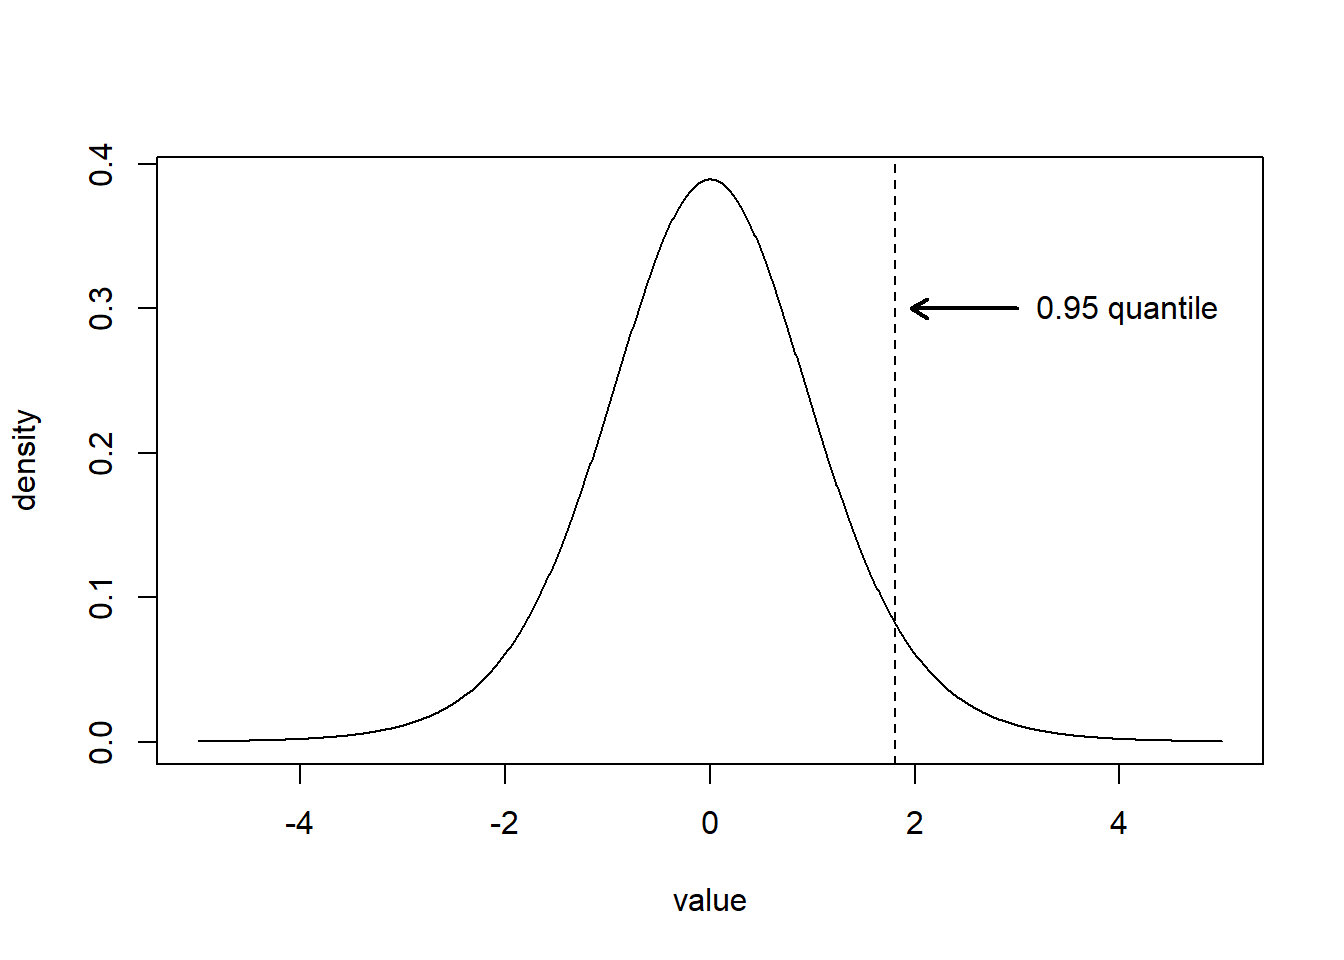
\includegraphics{A-Progessive-Introduction-to-Linear-Models_files/figure-latex/tquantile-1.pdf}
\caption{\label{fig:tquantile}The solid line shows the density of a \(t\) random variable with 10 degrees of freedom. The dashed vertical line indicates \(t^{0.05}_{10}\), the 0.95 quantile of a \(t\) distribution with 10 degrees of freedom. The area to the left of the line is 0.95 while the area to the right is 0.05.}
\end{figure}

We use the notation \(F_{\nu_1, \nu_2}\) to denote a random variable
having an \(F\) distribution with \(\nu_1\) numerator degrees of freedom and
\(\nu_2\) denominator degrees of freedom. We let
\(F^{\alpha}_{\nu_1,\nu_2}\) denote the \(1-\alpha\) quantile of an \(F\)
random variables with \(\nu_1\) numerator degrees of freedom and \(\nu_2\)
denominator degrees of freedom. In fact, \([t_{\nu}]^2=F_{1,\nu}\), i.e.,
the square of a \(t\) random variable with \(\nu\) degrees of freedom is
equivalent to an \(F\) random variable with \(1\) numerator degree of
freedom and \(\nu\) denominator degrees of freedom.

\hypertarget{properties-betahat}{%
\section{Properties of the OLS estimator}\label{properties-betahat}}

We continue by reviewing some of the properties of
\(\hat{\boldsymbol{\beta}}\), the OLS estimator of the regression
coefficient vector.

We assume that
\[
\mathbf{y} = \mathbf{X}\boldsymbol{\beta}+\boldsymbol{\epsilon}, \label{eq:model-def-inference}
\] using standard matrix notation.

We also assume that the model in Equation \eqref{eq:model-def-inference}
is correct (i.e., we have correctly specified the true model that
generated the data) and that
\[
\boldsymbol{\epsilon}\mid \mathbf{X}\sim \mathcal{N}(\mathbf{0}_{n\times 1},\sigma^2 \mathbf{I}_{n\times n}).  \label{eq:error-assumption-inference}
\]
This assumption applies to all errors, so we believe that all errors, observed and future, will have mean 0, variance \(\sigma^2\), will be uncorrelated, and have a normal distribution.

Under these assumptions, we showed in Chapter \ref{linear-model-theory}
that

\[
\mathbf{y}\mid \mathbf{X}\sim \mathcal{N}(\mathbf{X}\boldsymbol{\beta}, \sigma^2 \mathbf{I}_{n\times n}).
\]
and
\[\hat{\boldsymbol{\beta}}\mid \mathbf{X} \sim \mathcal{N}(\boldsymbol{\beta}, \sigma^2(\mathbf{X}^T\mathbf{X})^{-1}).
\label{eq:prop-betahat}
\]

\hypertarget{parametric-confidence-intervals-for-regression-coefficients}{%
\section{Parametric confidence intervals for regression coefficients}\label{parametric-confidence-intervals-for-regression-coefficients}}

\hypertarget{tci}{%
\subsection{\texorpdfstring{Standard \(t\)-based confidence intervals}{Standard t-based confidence intervals}}\label{tci}}

Under the assumptions in Equations \eqref{eq:model-def-inference} and
\eqref{eq:error-assumption-inference}, we can prove (though we won't)
that
\[
\frac{\hat{\beta}_j-\beta_j}{\hat{\mathrm{se}}(\hat{\beta}_j)}\sim t_{n-p}, \quad j=0,1,\ldots,p-1,
\]

where
\(\hat{\mathrm{se}}(\hat{\beta}_j)=\hat{\sigma}(\mathbf{X}^T\mathbf{X})^{-1}_{j+1,j+1}\)
is the estimated standard error of \(\hat{\beta}_j\). Recall that
estimated standard error is the estimated standard deviation of the
sampling distribution of \(\hat{\beta}_j\). Also, recall that the notation
\((\mathbf{X}^T\mathbf{X})^{-1}_{j+1,j+1}\) indicates the element in row
\(j+1\), column \(j+1\), of the matrix \((\mathbf{X}^T\mathbf{X})^{-1}\).
Thus, \((\hat{\beta}_j-\beta_j)/\hat{\mathrm{se}}(\hat{\beta}_j)\) is a
pivotal quantity with a \(t\) distribution, and it can be used to derive a
confidence interval

A confidence interval for \(\beta_j\) with confidence level \(1-\alpha\) is
given by the expression
\[
\hat{\beta}_j \pm t^{\alpha/2}_{n-p} \hat{\mathrm{se}}(\hat{\beta}_j),\quad j=0,2,\ldots,p-1.
\label{eq:t-ci-betas}
\]
It is critical to note that the \(1-\alpha\) confidence level refers to
the procedure for a single interval, not the family of intervals we can
produce for all \(p\) coefficients. We discuss this issue in more detail
in Section \ref{mcp}.

The \texttt{confint} function returns confidence intervals for the regression
coefficients of a fitted model. Technically, the \texttt{confint} function is a
generic function that has methods for many different object classes, but
we only discuss its usage with \texttt{lm} objects. The \texttt{confint} function has
3 main arguments:

\begin{itemize}
\tightlist
\item
  \texttt{object}: a fitted model object. In our case, the object produced by the \texttt{lm} function.
\item
  \texttt{parm}: a vector of numbers or names indicating the parameters for which we want to construct confidence intervals. By default, confidence intervals are constructed for all parameters.
\item
  \texttt{level}: the confidence level desired for the confidence interval. The default value is \texttt{0.95}, which will produce 95\% confidence intervals.
\end{itemize}

We once again use the \texttt{penguins} data from the \textbf{palmerpenguins}
package (\protect\hyperlink{ref-R-palmerpenguins}{Horst, Hill, and Gorman 2022}) to illustrate what we have learned. Consider
the regression model
\[
\begin{aligned}
&E(\mathtt{bill\_length\_mm}\mid \mathtt{body\_mass\_g}, \mathtt{flipper\_length\_mm}) \\
&=\beta_0+\beta_1 \mathtt{body\_mass\_g} + \beta_2 \mathtt{flipper\_length\_mm}.
\end{aligned}
\]

We estimate the parameters of this model in R using the code below.

\begin{Shaded}
\begin{Highlighting}[]
\CommentTok{\# load data}
\FunctionTok{data}\NormalTok{(penguins, }\AttributeTok{package =} \StringTok{"palmerpenguins"}\NormalTok{)}
\CommentTok{\# fit model}
\NormalTok{mlmod }\OtherTok{\textless{}{-}} \FunctionTok{lm}\NormalTok{(bill\_length\_mm }\SpecialCharTok{\textasciitilde{}}\NormalTok{ body\_mass\_g }\SpecialCharTok{+}\NormalTok{ flipper\_length\_mm, }\AttributeTok{data =}\NormalTok{ penguins)}
\end{Highlighting}
\end{Shaded}

We obtain the 95\% confidence intervals for the 3 regression coefficients
by running the code below.

\begin{Shaded}
\begin{Highlighting}[]
\FunctionTok{confint}\NormalTok{(mlmod)}
\DocumentationTok{\#\#                           2.5 \%      97.5 \%}
\DocumentationTok{\#\# (Intercept)       {-}1.244658e+01 5.573192182}
\DocumentationTok{\#\# body\_mass\_g       {-}4.534709e{-}04 0.001777908}
\DocumentationTok{\#\# flipper\_length\_mm  1.582365e{-}01 0.285494420}
\end{Highlighting}
\end{Shaded}

The 95\% confidence interval for the intercept parameter is {[}-12.45,
5.58{]}. We are 95\% confident that the mean penguin bill length is between
-12.25 and 5.58 mm for a penguin with a body mass of 0 g and a flipper
length of 0 mm. (This really isn't sensible).

The 95\% confidence interval for the \texttt{body\_mass\_g} coefficient is
{[}-0.00046, 0.002{]}. We are 95\% confident the regression coefficient for
\texttt{body\_mass\_g} is between -0.00046 and 0.002, assuming the
\texttt{flipper\_length\_mm} regressor is also in the model.

If we wanted to get the 90\% confidence interval for the
\texttt{flipper\_length\_mm} coefficient by itself, we could use either of the
commands shown below.

\begin{Shaded}
\begin{Highlighting}[]
\CommentTok{\# two styles for determining the CI for a single parameter (at a 90\% level)}
\FunctionTok{confint}\NormalTok{(mlmod, }\AttributeTok{parm =} \DecValTok{3}\NormalTok{, }\AttributeTok{level =} \FloatTok{0.90}\NormalTok{)}
\DocumentationTok{\#\#                         5 \%      95 \%}
\DocumentationTok{\#\# flipper\_length\_mm 0.1685112 0.2752197}
\FunctionTok{confint}\NormalTok{(mlmod, }\AttributeTok{parm =} \StringTok{"flipper\_length\_mm"}\NormalTok{, }\AttributeTok{level =} \FloatTok{0.90}\NormalTok{)}
\DocumentationTok{\#\#                         5 \%      95 \%}
\DocumentationTok{\#\# flipper\_length\_mm 0.1685112 0.2752197}
\end{Highlighting}
\end{Shaded}

We discuss how to ``manually'' construct these intervals using R in
Section \ref{manual-t-cis}.

\hypertarget{mcp}{%
\subsection{The multiple comparisons problem}\label{mcp}}

Our linear models typically have multiple regression coefficients, and thus, we typically want to construct confidence intervals for all of the coefficients.

While individual confidence intervals have utility in providing us with plausible values of the unknown coefficients, the confidence level of the procedure described in Section \ref{tci} is only valid for a single interval. Since we are constructing multiple intervals, the simultaneous confidence level of the procedure for the family of intervals is less than \(1-\alpha\). This is an example of the multiple comparisons problem.

A \textbf{multiple comparisons problem} occurs anytime we make multiple inferences (confidence intervals, hypothesis tests, prediction intervals, etc.). We are more likely to draw erroneous conclusions if we do not adjust for the fact that we are making multiple inferential statements. E.g., a confidence interval procedure with level 0.95 will produce intervals that contain the target parameter with probability 0.95. If we construct two confidence intervals with level 0.95, then the family-wise confidence level (i.e., the probability that both intervals simultaneously contain their respective target parameters) will be less than 0.95. (We can guarantee that our family-wise confidence level will be at least 0.90, but we can't determine the exact value without more information). In general, the \textbf{family-wise confidence level} is the probability that all intervals under consideration simultaneously contain their target parameter. The family-wise confidence level is also known as the \textbf{simultaneous} or \textbf{overall} confidence level.

A \textbf{multiple comparisons procedure} is a procedure designed to adjust for multiple inferences. In the context of confidence intervals, a multiple comparisons procedure will produce a family of intervals that have a family-wise confidence level above some threshold. We discuss two basic multiple comparisons procedures for confidence
intervals below.

\hypertarget{adjusted-cis-betas}{%
\subsection{Adjusted confidence intervals for regression coefficients}\label{adjusted-cis-betas}}

Bonferroni (\protect\hyperlink{ref-bonferroni1936}{1936}) proposed a simple multiple comparisons procedure that is applicable in many contexts. This general procedure is known as the \textbf{Bonferroni correction}. We describe its application below.

Suppose we are constructing \(k\) confidence intervals simultaneously. We control the family-wise confidence level of our intervals at \(1-\alpha\) if we construct the individual confidence intervals with the level \(1-\alpha/k\). We sketch a proof of this below.

Boole's inequality (\protect\hyperlink{ref-boole}{Boole 1847}) states that for a countable set of events \(A_1, A_2, A_3 \ldots\),
\[P(\cup_{j=1}^\infty A_j) \leq \sum_{j=1}^\infty P(A_j).\] This is a
generalization of the fact that
\[
P(A \cup B) = P(A) + P(B) - P(A\cap B) \leq P(A) + P(B)
\]
for two events \(A\) and \(B\). We can use Boole's inequality to show that the Bonferroni correction controls the family-wise confidence level of our confidence intervals at \(1-\alpha\).

Suppose that we construct a family of \(k\) confidence intervals with individual confidence level \(1-\alpha/k\) (and all assumptions are satisfied.) Then the probability that the confidence interval procedure for a specific interval doesn't contain the target parameter is
\(\alpha/k\). Then
\[
\begin{aligned}
& P(\mbox{All }k\mbox{ intervals contain the target parameter}) \\
& = 1 - P(\mbox{At least one of the }k\mbox{ intervals misses the target parameter}) \\
& = 1 - P(\cup_{j=1}^k \mbox{interval }j\mbox{ misses the target parameter}) \\
& \geq 1 - \sum_{j=1}^k P(\mbox{interval }j\mbox{ misses the target parameter}) \\
& = 1 - k(\alpha/k) \\
&= 1-\alpha.
\end{aligned}
\]
Thus, the family-wise confidence level of all \(k\) intervals is AT LEAST \(1-\alpha\) when the Bonferroni correction is used.

The Bonferroni correction is known to be conservative, which means that the family-wise confidence level is typically much larger than \(1-\alpha\). This might sound like a desirable property, but conservative methods can have low power. In the context of our confidence intervals, this means our intervals are much wider than they need to be, so we aren't able to draw precise conclusions about the plausible values of our regression coefficients.

Let's construct simultaneous confidence intervals for our \texttt{penguins} example using the Bonferroni correction. If we want to control the family-wise confidence level of our \(k=3\) intervals at \(0.95\), then \(\alpha = 0.05\) and the Bonferroni correction suggests that we should construct the individual intervals at a confidence level of \(1-0.05/3=0.983\). We construct the Bonferroni-adjusted confidence intervals using the code below.

\begin{Shaded}
\begin{Highlighting}[]
\CommentTok{\# Simultaneous 95\% confidence intervals for mlmod}
\FunctionTok{confint}\NormalTok{(mlmod, }\AttributeTok{level =} \DecValTok{1} \SpecialCharTok{{-}} \FloatTok{0.05}\SpecialCharTok{/}\DecValTok{3}\NormalTok{)}
\DocumentationTok{\#\#                         0.833 \%    99.167 \%}
\DocumentationTok{\#\# (Intercept)       {-}1.445714e+01 7.583749811}
\DocumentationTok{\#\# body\_mass\_g       {-}7.024372e{-}04 0.002026874}
\DocumentationTok{\#\# flipper\_length\_mm  1.440377e{-}01 0.299693234}
\end{Highlighting}
\end{Shaded}

Alternatively, we can use the \texttt{confint\_adjust} function from the \textbf{api2lm} package (\protect\hyperlink{ref-R-api2lm}{French 2022}) to construct this interval. The \texttt{confint\_adjust} function works identically to the \texttt{confint} function except that it has an additional argument to indicate the type of adjustment to make when constructing the confidence intervals. Specifying \texttt{method\ =\ "bonferroni"} will produce Bonferroni-corrected intervals, as demonstrated in the code below.

\begin{Shaded}
\begin{Highlighting}[]
\FunctionTok{library}\NormalTok{(api2lm)}
\FunctionTok{confint\_adjust}\NormalTok{(mlmod, }\AttributeTok{method =} \StringTok{"bonferroni"}\NormalTok{)}
\DocumentationTok{\#\# }
\DocumentationTok{\#\# Bonferroni{-}adjusted confidence intervals}
\DocumentationTok{\#\# }
\DocumentationTok{\#\# Family{-}wise confidence level of at least 0.95 }
\DocumentationTok{\#\# }
\DocumentationTok{\#\#               term           lwr         upr}
\DocumentationTok{\#\#        (Intercept) {-}1.445714e+01 7.583749811}
\DocumentationTok{\#\#        body\_mass\_g {-}7.024372e{-}04 0.002026874}
\DocumentationTok{\#\#  flipper\_length\_mm  1.440377e{-}01 0.299693234}
\end{Highlighting}
\end{Shaded}

Working and Hotelling (\protect\hyperlink{ref-workinghotelling}{1929}) developed another multiple comparisons procedure that can be used to preserve the family-wise confidence level of the intervals at \(1-\alpha\). The Working-Hotelling multiple comparisons procedure is valid for ALL linear combination of the regression coefficients, meaning that we can construct an arbitrarily large number of confidence intervals for linear combinations of the regression coefficients with this procedure and the family-wise confidence level will be at least \(1-\alpha\) (\protect\hyperlink{ref-alr4}{Weisberg 2014}).

The Working-Hotelling procedure guarantees that if we construct the individual confidence intervals in the following way, then the family-wise confidence level will be at least \(1-\alpha\):
\[
\hat{\beta}_j \pm \sqrt{p F^\alpha_{p,n-p}} \hat{\mathrm{se}}(\hat{\beta}_j),\quad j=0,2,\ldots,p-1. \label{eq:wh-ci-betas}
\]

The \texttt{confint\_adjust} function from the \textbf{api2lm} package will produce these intervals when setting the \texttt{method} argument to \texttt{"wh"}. We construct Working-Hotelling-adjusted intervals with family-wise confidence level of at least 0.95 for the \texttt{penguins} example using the
code below.

\begin{Shaded}
\begin{Highlighting}[]
\CommentTok{\# 95\% family{-}wise CIs using Working{-}Hotelling}
\FunctionTok{confint\_adjust}\NormalTok{(mlmod, }\AttributeTok{method =} \StringTok{"wh"}\NormalTok{)}
\DocumentationTok{\#\# }
\DocumentationTok{\#\# Working{-}Hotelling{-}adjusted confidence intervals}
\DocumentationTok{\#\# }
\DocumentationTok{\#\# Family{-}wise confidence level of at least 0.95 }
\DocumentationTok{\#\# }
\DocumentationTok{\#\#               term           lwr         upr}
\DocumentationTok{\#\#        (Intercept) {-}1.630614e+01 9.432751051}
\DocumentationTok{\#\#        body\_mass\_g {-}9.313981e{-}04 0.002255835}
\DocumentationTok{\#\#  flipper\_length\_mm  1.309798e{-}01 0.312751116}
\end{Highlighting}
\end{Shaded}

In this example, the Bonferroni-adjusted intervals are narrower than the Working-Hotelling-adjusted intervals. The Working-Hotelling intervals tends to be narrower for small \(p\) (e.g., \(p=1\) or \(2\)) and small \(n-p\) (e.g., \(n-p = 1\) or \(2\)) (\protect\hyperlink{ref-bon_vs_scheffe}{Mi and Sampson 1993}). Additionally, as the number of intervals increases, the Working-Hotelling intervals will eventually be narrower than the Bonferroni-adjusted intervals.

\hypertarget{prediction-mean-response-versus-new-response}{%
\section{Prediction: mean response versus new response}\label{prediction-mean-response-versus-new-response}}

It is common to make two types of predictions in a regression context: prediction of a mean response and prediction of a new response. In either context, we want to make predictions with respect to a specific
combination of regressor values, which we denote \(\mathbf{x}_0\). Using our previous notation, the mean response for a specific combination of regressors is denoted \(E(Y\mid \mathbb{X}=\mathbf{x}_0)\). We do not have
notation to describe a new response for a specific combination of regressor values, so we will use the notation \(Y(\mathbf{x}_0)\).

\(E(Y\mid \mathbb{X}=\mathbf{x}_0)\) represents the average response when the regressor values are \(\mathbf{x}_0\). Conceptually, this is the number we would get if were able to determine the average of an infinite number of responses with regressor values being fixed at \(\mathbf{x}_0\).

\(Y(\mathbf{x}_0)\) represents the actual response we will will observe for a new observation with regressor values \(\mathbf{x}_0\). Conceptually, we can think of \(Y(\mathbf{x}_0)\) as the mean response for that combination of regressor values plus some error, or more formally,
\[
Y(\mathbf{x}_0)=E(Y\mid \mathbb{X}=\mathbf{x}_0)+\epsilon(\mathbf{x}_0),
\]
where \(\epsilon(\mathbf{x_0})\) denotes the error for our new observation.

Suppose we want to rent a new apartment or buy a new house. If we look through the available listings, we will likely filter our search results by certain characteristics. We might limit our search to dwellings with 3 bedrooms, 2 bathrooms, that are within a certain distance of public transportation, and have a certain amount of square footage. If we averaged the monthly rent or asking price of all the dwellings matching our specifications, then that would be an approximation of the mean response (we would need all the possible dwellings matching those considerations to get the true average). This average would give us an idea of the ``typical'' price of dwellings with those characteristics. On the other hand, we likely want to know the price of the dwelling we actually end up in. This is the ``new response'' we want to predict.

Though we can discuss predictions for both the mean response and a new response, it is common to distinguish the two scenarios by using the terminology ``estimating the mean response'' to refer to prediction of the the mean and ``prediction a new response'' when we want to predict a new observation. We use this convention in what follows to distinguish the two contexts.

\hypertarget{parametric-ci-mean-response}{%
\section{Confidence interval for the mean response}\label{parametric-ci-mean-response}}

Consider a typical linear regression model with \(p\) regression
coefficients given by
\[E(Y|\mathbb{X})=\beta_0+\beta_1 X_1 + \ldots \beta_{p-1} X_{p-1}.\]We
want to estimate the mean response for a specific combination of
regressor values. The mean response for that combination of regressors
is obtained via the equivalent expressions \[
\begin{aligned}
E(Y\mid \mathbb{X}=\mathbf{x}_0) &= \beta_0 + \sum_{j=1}^{p-1}x_{0,j}\beta_j \\
&= \mathbf{x}_0^T \boldsymbol{\beta}. 
\end{aligned}
\]

To simplify our notation, we drop the ``\(\mathbb{X}=\)'' in our discussion below, so
\(E(Y\mid \mathbb{X}=\mathbf{x}_0)\equiv E(Y\mid \mathbf{x}_0)\).

What does \(E(Y\mid \mathbf{x}_0)\) represent? It represents the average response we will observe if we somehow managed to observe infinitely many responses with \(\mathbb{X}=\mathbf{x}_0\).

The Gauss-Markov Theorem discussed in Chapter
\ref{linear-model-estimation} indicates that the best linear unbiased
estimator of the mean response is given by the equation\[
\begin{aligned}
\hat{E}(Y\mid \mathbf{x}_0) &= \hat{\beta}_0 + \sum_{j=1}^{p-1}x_{0,j}\hat{\beta}_j \\
&= \mathbf{x}_0^T \hat{\boldsymbol{\beta}}, 
\end{aligned}
\]

which replaces the unknown, true coefficients by their OLS estimates.

We want to create a confidence interval for \(E(Y\mid \mathbf{x}_0)\). If we divide the estimation error of the mean response, i.e., \(E(Y\mid \mathbf{x}_0)-\hat{E}(Y\mid \mathbf{x}_0)\), by its estimated standard deviation, then we obtain a pivotal quantity. More specifically, we have \[
\frac{E(Y\mid \mathbf{x}_0)-\hat{E}(Y\mid \mathbf{x}_0)}{\sqrt{\hat{\mathrm{var}}\left(E(Y\mid \mathbf{x}_0)-\hat{E}(Y\mid \mathbf{x}_0)\right)}} = \frac{E(Y\mid \mathbf{x}_0)- \mathbf{x}_0 \hat{\boldsymbol{\beta}}}{ \hat{\mathrm{se}}(\mathbf{x}_0\hat{\boldsymbol{\beta}})}\sim t_{n-p},
\]
with
\[
\hat{\mathrm{se}}(\mathbf{x}_0^T\hat{\boldsymbol{\beta}})=\hat{\sigma}\sqrt{\mathbf{x}_0^T (\mathbf{X}^T \mathbf{X})^{-1}\mathbf{x}_0}. \label{eq:sehat-est-mean}
\]
A confidence interval for \(E(Y\mid \mathbf{x}_0)\) with confidence
level \(1-\alpha\) is given by the expression
\[
\mathbf{x}_0\hat{\boldsymbol{\beta}} \pm t^{\alpha/2}_{n-p} \hat{\mathrm{se}}(\mathbf{x}_0\hat{\boldsymbol{\beta}}). \label{eq:t-ci-mean-response}
\]

The \texttt{predict} function is a generic function used to make predictions
based on fitted models. We can use this function to estimate the mean
response for multiple combinations of predictor variables, compute the
estimated standard error of each estimate, and obtain confidence
intervals for the mean response. The primary arguments to the \texttt{lm}
method for \texttt{predict} are:

\begin{itemize}
\tightlist
\item
  \texttt{object}: A fitted model from the \texttt{lm} function.
\item
  \texttt{newdata}: A data frame of predictor values. All predictors used in the formula used to fit \texttt{object} must be provided. Each row contains the predictor values for the mean response we want to estimate. If this is not provided, then the fitted values for each observation are returned.
\item
  \texttt{se.fit}: A logical value indicating whether we want to explicitly
  compute the standard errors of each estimated mean, i.e.,
  \(\hat{\mathrm{se}}(\hat{E}(Y\mid \mathbf{x}_0))\) for each estimate.
\item
  \texttt{interval}: The type of interval to compute. The default is \texttt{none},
  meaning no interval is provided. Setting \texttt{interval\ =\ "confidence"}
  will return a confidence interval for the mean response associated
  with each row of \texttt{newdata}. Setting \texttt{interval\ =\ "prediction"} will
  return a prediction interval for a new response, which we will
  discuss in the next section.
\item
  \texttt{level}: The confidence level of the interval.
\end{itemize}

Run \texttt{?predict.lm} in the Console for additional details about this
function.

We will estimate the mean response for the parallel lines model
previously fit to the \texttt{penguins} data. We do this to emphasize the fact
that the \texttt{predict} function asks you to specify the values of the
\emph{predictor} variables for each estimate you want to make, not the
complete set of regressors.

Recall that in Section \ref{s:penguins-mlr2}, we fit a parallel lines
model to the \texttt{penguins} data that used both \texttt{body\_mass\_g} and \texttt{species}
to explain the behavior of \texttt{bill\_length\_mm}. Letting \(D_C\) denote the
indicator variable for the \texttt{Chinstrap} level and \(D_G\) denote the
indicator variable for the \texttt{Gentoo} level, the fitted parallel lines
model was \[
\begin{aligned}
&\hat{E}(\mathtt{bill\_length\_mm} \mid \mathtt{body\_mass\_g}, \mathtt{species})\\
&= 24.92 + 0.004 \mathtt{body\_mass\_g} + 9.92 D_C + 3.56 D_G.
\end{aligned}
\] We fit this model below, assigning it the name \texttt{lmodp}.

\begin{Shaded}
\begin{Highlighting}[]
\CommentTok{\# fit parallel lines model to penguins data}
\NormalTok{lmodp }\OtherTok{\textless{}{-}} \FunctionTok{lm}\NormalTok{(bill\_length\_mm }\SpecialCharTok{\textasciitilde{}}\NormalTok{ body\_mass\_g }\SpecialCharTok{+}\NormalTok{ species,}
            \AttributeTok{data =}\NormalTok{ penguins)}
\FunctionTok{coef}\NormalTok{(lmodp)}
\DocumentationTok{\#\#      (Intercept)      body\_mass\_g speciesChinstrap }
\DocumentationTok{\#\#     24.919470977      0.003748497      9.920884113 }
\DocumentationTok{\#\#    speciesGentoo }
\DocumentationTok{\#\#      3.557977539}
\end{Highlighting}
\end{Shaded}

Let's estimate the mean response for the ``typical'' \texttt{body\_mass\_g} of each \texttt{species}. We compute the mean \texttt{body\_mass\_g} of each \texttt{species} using the code below, assigning the resulting data frame the name \texttt{newpenguins}. We use the \texttt{group\_by} and \texttt{summarize} functions from the \textbf{dplyr} package (\protect\hyperlink{ref-R-dplyr}{Wickham, François, et al. 2023}) to simplify this process.

\begin{Shaded}
\begin{Highlighting}[]
\CommentTok{\# mean body\_mass\_g of each species}
\NormalTok{newpenguins }\OtherTok{\textless{}{-}}\NormalTok{ penguins }\SpecialCharTok{|\textgreater{}}
\NormalTok{  dplyr}\SpecialCharTok{::}\FunctionTok{group\_by}\NormalTok{(species) }\SpecialCharTok{|\textgreater{}}
\NormalTok{  dplyr}\SpecialCharTok{::}\FunctionTok{summarize}\NormalTok{(}\AttributeTok{body\_mass\_g =} \FunctionTok{mean}\NormalTok{(body\_mass\_g, }\AttributeTok{na.rm =} \ConstantTok{TRUE}\NormalTok{))}
\NormalTok{newpenguins}
\DocumentationTok{\#\# \# A tibble: 3 x 2}
\DocumentationTok{\#\#   species   body\_mass\_g}
\DocumentationTok{\#\#   \textless{}fct\textgreater{}           \textless{}dbl\textgreater{}}
\DocumentationTok{\#\# 1 Adelie          3701.}
\DocumentationTok{\#\# 2 Chinstrap       3733.}
\DocumentationTok{\#\# 3 Gentoo          5076.}
\end{Highlighting}
\end{Shaded}

We now have a data frame with variables for the two predictors, \texttt{species} and \texttt{body\_mass\_g} , used to fit \texttt{lmodp}. Each row of \texttt{newpenguins} contains the mean \texttt{body\_mass\_g} for each level of \texttt{species} and is suitable for use in the \texttt{predict} function.

In the code below, we estimate the mean \texttt{flipper\_length\_mm} based on the fitted model in \texttt{lmodp} for the mean \texttt{body\_mass\_g} of each level of \texttt{species}. We also choose to compute the estimated standard errors of
each estimate by setting the \texttt{se.fit} argument to \texttt{TRUE}.

\begin{Shaded}
\begin{Highlighting}[]
\CommentTok{\# estimate mean and standard error for 3 combinations of predictors}
\FunctionTok{predict}\NormalTok{(lmodp, }\AttributeTok{newdata =}\NormalTok{ newpenguins, }\AttributeTok{se.fit =} \ConstantTok{TRUE}\NormalTok{)}
\DocumentationTok{\#\# $fit}
\DocumentationTok{\#\#        1        2        3 }
\DocumentationTok{\#\# 38.79139 48.83382 47.50488 }
\DocumentationTok{\#\# }
\DocumentationTok{\#\# $se.fit}
\DocumentationTok{\#\#         1         2         3 }
\DocumentationTok{\#\# 0.1955643 0.2914228 0.2166833 }
\DocumentationTok{\#\# }
\DocumentationTok{\#\# $df}
\DocumentationTok{\#\# [1] 338}
\DocumentationTok{\#\# }
\DocumentationTok{\#\# $residual.scale}
\DocumentationTok{\#\# [1] 2.403134}
\end{Highlighting}
\end{Shaded}

An Adelie penguin with a body mass of 3700.662 g is estimated to have a mean flipper length of 38.79 mm with an estimated standard error of 0.196 mm. A Chinstrap penguin with a body mass of 3733.09 g is estimated to have a mean flipper length of 48.83 mm with an estimated standard error of 0.29 mm. A Gentoo penguin with a body mass of 5076.02 g is estimated to have a mean flipper length of 47.50 mm with an estimated standard error of 0.22 mm.

To create each 98\% confidence intervals for the mean response for each combination of predictors, we specify \texttt{level\ =\ 0.98} and \texttt{interval\ =\ "confidence"} in the \texttt{predict} function in the code below.

\begin{Shaded}
\begin{Highlighting}[]
\FunctionTok{predict}\NormalTok{(lmodp, }\AttributeTok{newdata =}\NormalTok{ newpenguins, }\AttributeTok{level =} \FloatTok{0.98}\NormalTok{, }\AttributeTok{interval =} \StringTok{"confidence"}\NormalTok{)}
\DocumentationTok{\#\#        fit      lwr      upr}
\DocumentationTok{\#\# 1 38.79139 38.33427 39.24851}
\DocumentationTok{\#\# 2 48.83382 48.15264 49.51500}
\DocumentationTok{\#\# 3 47.50488 46.99840 48.01136}
\end{Highlighting}
\end{Shaded}

The 98\% confidence interval for the mean flipper length of an Adelie penguin with a body mass of 3700.662 g is {[}38.33, 39.25{]}. We are 98\% confident that the mean flipper length of Adelie penguins with a body mass of 3700.662 is between 38.33 g and 39.25 g. Note: we are constructing a confidence interval for the mean flipper length of ALL
Adelie penguins with this body mass, i.e., for
\[
E(\mathtt{flipper\_length\_mm}\mid \mathtt{body\_mass\_g} = 3700.662, \mathtt{species} = \mathtt{Adelie}),
\]
which is an unknown characteristic of the population of all Adelie penguins. Similarly, the 98\% confidence interval for the mean flipper length of Chinstrap penguins with a body mass of 3733.09 g is {[}48.15, 49.52{]}. Lastly, the mean flipper length of Gentoo penguins with a body mass of 5076.02 g is {[}46.99, 48.02{]}.

We provide details about manually computing confidence intervals for the mean response in Section \ref{manual-calc-ci-mean-response}.

We are once again faced with a multiple comparisons problem because we are making 3 inferences. To control the family-wise confidence level of our intervals, we can use the Bonferroni or Working-Hotelling corrections previously discussed in Section \ref{adjusted-cis-betas}. Both corrections are implemented in the \texttt{predict\_adjust} function in the \textbf{api2lm} package, which is intended to work identically to the \texttt{predict} function, but produces intervals that adjust for multiple comparisons. The only additional argument is \texttt{method}, with choices \texttt{"none"} (no correction), \texttt{"bonferroni"} (Bonferroni adjustment), or \texttt{"wh"} (Working-Hotelling adjustment). We produce both types of adjusted intervals in the code below. The Bonferroni-adjusted confidence intervals are slightly narrower in this example.

\begin{Shaded}
\begin{Highlighting}[]
\CommentTok{\# bonferroni{-}adjusted confidence intervals for the mean response}
\FunctionTok{predict\_adjust}\NormalTok{(lmodp, }\AttributeTok{newdata =}\NormalTok{ newpenguins, }\AttributeTok{level =} \FloatTok{0.98}\NormalTok{,}
               \AttributeTok{interval =} \StringTok{"confidence"}\NormalTok{, }\AttributeTok{method =} \StringTok{"bonferroni"}\NormalTok{)}
\DocumentationTok{\#\# }
\DocumentationTok{\#\# Bonferroni{-}adjusted confidence intervals}
\DocumentationTok{\#\# }
\DocumentationTok{\#\# Family{-}wise confidence level of at least 0.98 }
\DocumentationTok{\#\# }
\DocumentationTok{\#\#        fit      lwr      upr}
\DocumentationTok{\#\# 1 38.79139 38.25751 39.32527}
\DocumentationTok{\#\# 2 48.83382 48.03826 49.62939}
\DocumentationTok{\#\# 3 47.50488 46.91335 48.09641}
\CommentTok{\# working{-}hotelling{-}adjusted confidence intervals for the mean response}
\FunctionTok{predict\_adjust}\NormalTok{(lmodp, }\AttributeTok{newdata =}\NormalTok{ newpenguins, }\AttributeTok{level =} \FloatTok{0.98}\NormalTok{,}
               \AttributeTok{interval =} \StringTok{"confidence"}\NormalTok{, }\AttributeTok{method =} \StringTok{"wh"}\NormalTok{)}
\DocumentationTok{\#\# }
\DocumentationTok{\#\# Working{-}Hotelling{-}adjusted confidence intervals}
\DocumentationTok{\#\# }
\DocumentationTok{\#\# Family{-}wise confidence level of at least 0.98 }
\DocumentationTok{\#\# }
\DocumentationTok{\#\#        fit      lwr      upr}
\DocumentationTok{\#\# 1 38.79139 38.11858 39.46420}
\DocumentationTok{\#\# 2 48.83382 47.83122 49.83642}
\DocumentationTok{\#\# 3 47.50488 46.75941 48.25035}
\end{Highlighting}
\end{Shaded}

\hypertarget{pi-new-response}{%
\section{Prediction interval for a new response}\label{pi-new-response}}

We once again assume the regression model
\[
E(Y|\mathbb{X})=\beta_0+\beta_1 X_1 + \ldots \beta_{p-1} X_{p-1}.
\]
We want to predict a new response for a specific combination of regressor values, \(\mathbf{x}_0\). The new response will be the mean response for that combination of regressors, \(E(Y\mid \mathbf{x}_0)\), plus the error for that observation, \(\epsilon(\mathbf{x}_0)\), i.e.,
\[
Y(\mathbf{x}_0)=E(Y\mid \mathbf{x}_0) + \epsilon(\mathbf{x}_0).
\]

Thus, our predicted new response, \(\hat{Y}(\mathbf{x})\) is the estimated mean plus the estimated error, i.e.,
\[
\hat{Y}(\mathbf{x}_0)=\hat{E}(Y\mid \mathbf{x}_0) + \hat{\epsilon}(\mathbf{x}_0).
\]
We have already used \(\hat{E}(Y\mid \mathbf{x}_0)=\mathbf{x}_0^T\hat{\boldsymbol{\beta}}\) as the estimator for \(E(Y\mid \mathbf{x}_0)\) since it is the best linear unbiased estimator according to the Gauss-Markov theorem. What should we use for \(\hat{\epsilon}(\mathbf{x}_0)\)? In short, because all of the errors, \(\epsilon_1, \epsilon_2,\ldots, \epsilon_n, \epsilon(\mathbf{x}_0)\) are uncorrelated, our best guess is the mean value of the errors, which is zero. This is not true when the errors are correlated, but we do not discuss that in detail. Thus, the best predictor of a new response is
\[
\begin{aligned}
\hat{Y}(\mathbf{x}_0) &=\hat{E}(Y\mid \mathbf{x}_0) + \hat{\epsilon}(\mathbf{x}_0)\\
&= \mathbf{x}_0^T\hat{\boldsymbol{\beta}} + 0 \\
&= \mathbf{x}_0^T\hat{\boldsymbol{\beta}}.
\end{aligned}
\]

We want to create a prediction interval for \(Y(\mathbf{x}_0)\). A prediction interval is basically the same thing as a confidence interval, but the interval estimator is for a random variable instead of a parameter. If we divide the estimation error of the new response, i.e.,
\(Y(\mathbf{x}_0)-\hat{Y}(\mathbf{x}_0)\), by its estimated standard deviation, \(\widehat{\mathrm{sd}}(Y(\mathbf{x}_0)-\hat{Y}(\mathbf{x}_0))\), then we obtain a \(t\)-distributed pivotal quantity:
\[
\frac{Y(\mathbf{x}_0)-\hat{Y}(\mathbf{x}_0)}{\widehat{\mathrm{sd}}(Y(\mathbf{x}_0)-\hat{Y}(\mathbf{x}_0))} \sim t_{n-p},
\]
where
\[
\widehat{\mathrm{sd}}(Y(\mathbf{x}_0)-\hat{Y}(\mathbf{x}_0))=\hat{\sigma}\sqrt{1 + \mathbf{x}_0^T (\mathbf{X}^T \mathbf{X})^{-1}\mathbf{x}_0}. \label{eq:sdhat-pred-error}
\]
The standard deviation of the prediction error is sometimes known as the \textbf{standard error of prediction}, but we do not use that terminology. A detailed derivation of \(\widehat{\mathrm{sd}}(Y(\mathbf{x}_0)-\hat{Y}(\mathbf{x}_0))\) is provided in Section \ref{new-response-pi-calculations}.

There is a conceptual and mathematical relationship between the standard deviation of the estimation error for the mean response and the prediction error for a new observation. If we compare the expression for \(\hat{\mathrm{se}}(\hat{E}(Y\mid \mathbf{x}_0)) - E(Y\mid \mathbf{x}_0))\) in Equation \eqref{eq:sehat-est-mean} and \(\widehat{\mathrm{sd}}(Y(\mathbf{x}_0)-\hat{Y}(\mathbf{x}_0))\) in Equation \eqref{eq:sdhat-pred-error}, we see that \(\widehat{\mathrm{sd}}(Y(\mathbf{x}_0)-\hat{Y}(\mathbf{x}_0))\) has an extra ``1 +'' under the square root. Because of this, \emph{prediction intervals for a new response are always wider than a confidence interval for the mean response} when considering the same regressor values, \(\mathbf{x}_0\), and confidence level. Conceptually, prediction intervals are wider because there are two sources of uncertainty in our prediction: estimating the mean response and predicting the error of the new response. Estimating the mean response does not require us to predict the error of a new response, so the uncertainty of our estimate is less. We can see that this is formally true through the derivations provided in Section \ref{new-response-pi-calculations}.

A prediction interval for \(Y(\mathbf{x}_0)\) with confidence level \(1-\alpha\) is given by the expression
\[
\mathbf{x}_0\hat{\boldsymbol{\beta}} \pm t^{\alpha/2}_{n-p} \hat{\mathrm{sd}}(Y(\mathbf{x}_0)-\hat{Y}(\mathbf{x}_0)). \label{eq:t-pi-new-response}
\]

The \texttt{predict} function can be used to create predictions and prediction intervals for a new response in the same way that it can be used to estimate the mean response and produce associated confidence intervals. If the \texttt{interval} argument is \texttt{"none"}, then predictions for a new response are returned. As we have already seen, \(\hat{E}(Y\mid \mathbf{x}_0)\) and \(\hat{Y}(\mathbf{x}_0)\) are the same number. If the \texttt{interval} argument is \texttt{"prediction"}, then the predicted new response and associated prediction interval will be produced for each row of data supplied to the \texttt{newdata} argument.

Continuing the example started in Section \ref{parametric-ci-mean-response}, we want to predict the response value for new, unobserved penguins having the observed mean \texttt{body\_mass\_g} for each level of \texttt{species}. The fitted model is stored in \texttt{lmodp} and the data frame with the predictors for the new responses is stored in \texttt{newpenguins}. We print the coefficients of the fitted model and the data frame of new predictors below for clarity.

\begin{Shaded}
\begin{Highlighting}[]
\FunctionTok{coef}\NormalTok{(lmodp)}
\DocumentationTok{\#\#      (Intercept)      body\_mass\_g speciesChinstrap }
\DocumentationTok{\#\#     24.919470977      0.003748497      9.920884113 }
\DocumentationTok{\#\#    speciesGentoo }
\DocumentationTok{\#\#      3.557977539}
\NormalTok{newpenguins}
\DocumentationTok{\#\# \# A tibble: 3 x 2}
\DocumentationTok{\#\#   species   body\_mass\_g}
\DocumentationTok{\#\#   \textless{}fct\textgreater{}           \textless{}dbl\textgreater{}}
\DocumentationTok{\#\# 1 Adelie          3701.}
\DocumentationTok{\#\# 2 Chinstrap       3733.}
\DocumentationTok{\#\# 3 Gentoo          5076.}
\end{Highlighting}
\end{Shaded}

In the code below, we predict the \texttt{flipper\_length\_mm} for new penguins for the predictor values stored in \texttt{newpenguins} based on the fitted model in \texttt{lmodp}. We also construct the associated 99\% prediction intervals.

\begin{Shaded}
\begin{Highlighting}[]
\CommentTok{\# predict new response and compute prediction intervals}
\CommentTok{\# for 3 combinations of predictors}
\FunctionTok{predict}\NormalTok{(lmodp, }\AttributeTok{newdata =}\NormalTok{ newpenguins,}
        \AttributeTok{interval =} \StringTok{"prediction"}\NormalTok{, }\AttributeTok{level =} \FloatTok{0.99}\NormalTok{)}
\DocumentationTok{\#\#        fit      lwr      upr}
\DocumentationTok{\#\# 1 38.79139 32.54561 45.03718}
\DocumentationTok{\#\# 2 48.83382 42.56301 55.10464}
\DocumentationTok{\#\# 3 47.50488 41.25442 53.75534}
\end{Highlighting}
\end{Shaded}

An new Adelie penguin with a body mass of 3700.662 g is predicted to have a flipper length of 38.79 mm. We are 99\% confident that a new Adelie penguins with a body mass of 3700.662 g will have a flipper length between 32.54 mm and 45.04 mm. Similarly, the 99\% prediction interval for the flipper length of a new Chinstrap penguin with a body mass of 3733.09 g is {[}48.56, 55.11{]}. The flipper length of a new Gentoo penguin with a body mass of 5076.02 g is between 41.25 and 53.75 with a confidence level of 0.99.

Since we are making 3 predictions, our inferences suffer from the multiple comparisons problem. To control the family-wise confidence level of our intervals, we can use the Bonferroni correction with \(k=3\). The Working-Hotelling correction discussed in Section \ref{adjusted-cis-betas} does not apply to new responses. However, a similar adjustment proposed by Scheffé does apply (\protect\hyperlink{ref-alsm2005}{Kutner et al. 2005}). The prediction interval multiplier \(t^{\alpha/2}_{n-p}\) used for a single prediction interval with confidence level \(1-\alpha\) is replaced by
\(\sqrt{k F^{1-\alpha}_{k,n-p}}\) to control the family-wise confidence level at \(1-\alpha\) for a family of \(k\) prediction intervals. Recall that the Working-Hotelling multiplier was \(\sqrt{p F^{1-\alpha}_{p,n-p}}\). Thus, the Scheffé multiplier scales with the number of predictions being made while the Working-Hotelling multiplier scales with the number of estimated regression coefficients in the fitted model.

Both the Bonferroni and Scheffé multiple comparisons corrections are implemented in the \texttt{predict\_adjust} function in the \textbf{api2lm} package. In the prediction interval setting, we can choose the correction \texttt{method} argument to be \texttt{"none"} (no correction), \texttt{"bonferroni"} (Bonferroni adjustment), or \texttt{"scheffe"} (Scheffe adjustment). We produce both types of adjusted intervals in the code below. The Bonferroni-adjusted confidence intervals are slightly narrower in this example.

\begin{Shaded}
\begin{Highlighting}[]
\CommentTok{\# bonferroni{-}adjusted prediction intervals for new responses}
\FunctionTok{predict\_adjust}\NormalTok{(lmodp, }\AttributeTok{newdata =}\NormalTok{ newpenguins, }\AttributeTok{level =} \FloatTok{0.99}\NormalTok{,}
               \AttributeTok{interval =} \StringTok{"prediction"}\NormalTok{,}
               \AttributeTok{method =} \StringTok{"bonferroni"}\NormalTok{)}
\DocumentationTok{\#\# }
\DocumentationTok{\#\# Bonferroni{-}adjusted prediction intervals}
\DocumentationTok{\#\# }
\DocumentationTok{\#\# Family{-}wise confidence level of at least 0.99 }
\DocumentationTok{\#\# }
\DocumentationTok{\#\#        fit      lwr      upr}
\DocumentationTok{\#\# 1 38.79139 31.66373 45.91905}
\DocumentationTok{\#\# 2 48.83382 41.67760 55.99004}
\DocumentationTok{\#\# 3 47.50488 40.37188 54.63787}
\CommentTok{\# sheffe{-}adjusted prediction intervals for new responses}
\FunctionTok{predict\_adjust}\NormalTok{(lmodp, }\AttributeTok{newdata =}\NormalTok{ newpenguins, }\AttributeTok{level =} \FloatTok{0.99}\NormalTok{,}
               \AttributeTok{interval =} \StringTok{"prediction"}\NormalTok{,}
               \AttributeTok{method =} \StringTok{"scheffe"}\NormalTok{)}
\DocumentationTok{\#\# }
\DocumentationTok{\#\# Scheffe{-}adjusted prediction intervals}
\DocumentationTok{\#\# }
\DocumentationTok{\#\# Family{-}wise confidence level of at least 0.99 }
\DocumentationTok{\#\# }
\DocumentationTok{\#\#        fit      lwr      upr}
\DocumentationTok{\#\# 1 38.79139 30.60787 46.97492}
\DocumentationTok{\#\# 2 48.83382 40.61751 57.05014}
\DocumentationTok{\#\# 3 47.50488 39.31523 55.69453}
\end{Highlighting}
\end{Shaded}

\hypertarget{hypothesis-tests-for-a-single-regression-coefficient}{%
\section{Hypothesis tests for a single regression coefficient}\label{hypothesis-tests-for-a-single-regression-coefficient}}

If we assume we are fitting the multiple linear regression model in Equation \eqref{eq:model-def-inference}, then our model has \(p\) regression coefficient \(\beta_0, \beta_1, \ldots, \beta_{p-1}\). How would we perform a hypothesis test for exactly one of these regression coefficients?

Recall that if we make the assumptions in Equation
\eqref{eq:error-assumption-inference}, then

\begin{equation}
\frac{\hat{\beta}_j-\beta_j}{\hat{\mathrm{se}}(\hat{\beta}_j)}\sim t_{n-p}, \quad j=0,1,\ldots,p-1. \label{eq:pivot-t-betaj}
\end{equation}

Let's say we wish to test whether, for this model, \(\beta_j\) differs from some constant number \(c\) (typically, \(c=0\)). Let \(\boldsymbol{\beta}_{-j}=\boldsymbol{\beta}\setminus{\beta_j}\), i.e., \(\boldsymbol{\beta}_{-j}\) is the vector of all regression coefficients except \(\beta_j\). \(\boldsymbol{\beta}_{-j}\) has \(p-1\) elements. We can state the hypotheses we wish to test as
\[
\begin{aligned}
H_0: \beta_j &= c \mid \boldsymbol{\beta}_{-j}\in\mathbb{R}^{p-1} \\
H_a: \beta_j &\neq c \mid \boldsymbol{\beta}_{-j}\in\mathbb{R}^{p-1}.
\end{aligned}
\label{eq:betaj-H0Ha}
\]
The first part of the null hypothesis in Equation \eqref{eq:betaj-H0Ha} states that \(\beta_j = c\) while the first part of the alternative hypothesis assumes that \(\beta_j \neq c\). But what does the second half of the hypotheses mean? The vertical bar means ``assuming or conditional on'', similar to the notation you would see in conditional probabilities or distributions. What this means is that we are performing the hypothesis test while assuming that the other coefficients are some real number (possibly even zero). Why state this at all? Isn't it implicitly assumed? No.~We could perform a hypothesis test for \(\beta_j\) for many different models that have differing regressors. By writing out hypotheses in the style of Equation \eqref{eq:betaj-H0Ha}, we are being very clear that we are performing a test for \(\beta_j\) in the context of the model that has the regressors associated with \(\boldsymbol{\beta}_{-j}\).

How do the hypotheses in Equation \eqref{eq:betaj-H0Ha} affect the pivotal quantity in Equation \eqref{eq:pivot-t-betaj}? Under the null hypothesis, the statistic
\[
T_j = \frac{\hat{\beta}_j-c}{\hat{\mathrm{se}}(\hat{\beta}_j)} \sim t_{n-p}.
\]
Thus, the null distribution of \(T_j\) is a \(t\) distribution with \(n-p\) degrees of freedom. We emphasize that this is only true if the assumptions in Equation
\eqref{eq:error-assumption-inference} are true.

The p-value associated with this test is computed via the equation
\[
p\text{-value} = 2P(t_{n-p}\geq |T_j|).
\]
What if we wished to test a one-sided hypothesis? The p-value for a lower-tailed test is \(p\text{-value}=P(t_{n-p}\leq T_j)\) while the p-value for an upper-tailed test is \(p\text{-value}=P(t_{n-p}\geq T_j)\).

The fitted model
\[
\begin{aligned}
&E(\mathtt{bill\_length\_mm}\mid \mathtt{body\_mass\_g}, \mathtt{flipper\_length\_mm}) \\
&=\beta_0+\beta_1 \mathtt{body\_mass\_g} + \beta_2 \mathtt{flipper\_length\_mm}.
\end{aligned}
\]

is assigned the name \texttt{mlmod}. Suppose we want to test

\[
\begin{aligned}
H_0: &\beta_1 = 0 \mid \beta_0\in \mathbb{R}, \beta_2 \in \mathbb{R} \\
H_a: &\beta_1 \neq 0 \mid \beta_0\in \mathbb{R}, \beta_2 \in \mathbb{R}.
\end{aligned}
\]
R conveniently provides this information in the output of the \texttt{summary} function (specifically, the \texttt{coefficients} element if we don't want extra information). We extract this information from the \texttt{mlmod} object in the code below.

\begin{Shaded}
\begin{Highlighting}[]
\FunctionTok{summary}\NormalTok{(mlmod)}\SpecialCharTok{$}\NormalTok{coefficients}
\DocumentationTok{\#\#                        Estimate   Std. Error    t value}
\DocumentationTok{\#\# (Intercept)       {-}3.4366939266 4.5805531903 {-}0.7502792}
\DocumentationTok{\#\# body\_mass\_g        0.0006622186 0.0005672075  1.1675067}
\DocumentationTok{\#\# flipper\_length\_mm  0.2218654584 0.0323484492  6.8586119}
\DocumentationTok{\#\#                       Pr(\textgreater{}|t|)}
\DocumentationTok{\#\# (Intercept)       4.536070e{-}01}
\DocumentationTok{\#\# body\_mass\_g       2.438263e{-}01}
\DocumentationTok{\#\# flipper\_length\_mm 3.306943e{-}11}
\end{Highlighting}
\end{Shaded}

Moving from left to right, the first column (no name) indicates the coefficient term under consideration, the second column (\texttt{Estimate}) provides the estimated coefficients, the third column (\texttt{Std.\ Error}) provides the estimated standard error (\(\hat{\mathrm{se}}(\hat{\beta}_j)\)) for each coefficient, the fourth column (\texttt{t\ value}) provides the test statistic associated with testing \(H_0: \beta_j = 0 \mid \boldsymbol{\beta}_{-j} \in \mathbb{R}^{p-1}\) versus a suitable alternative for each coefficient, while the final column (\texttt{Pr(\textgreater{}\textbar{}t\textbar{})}) provides the two-tailed p-value associated with this test.

Thus, for our test of the \texttt{body\_mass\_g} coefficient, the test statistic is \(T_2 = 1.17\) and the associated p-value is 0.024. There is moderate evidence that the coefficient for \texttt{body\_mass\_g} differs from zero, assuming the model also allows for the inclusion of the intercept and \texttt{flipper\_length\_mm} coefficients.

\hypertarget{hypothesis-tests-for-multiple-regression-coefficients}{%
\section{Hypothesis tests for multiple regression coefficients}\label{hypothesis-tests-for-multiple-regression-coefficients}}

Suppose we have have a standard linear regression model with
\(p\) regression coefficients such as the one defined in Equation \eqref{eq:model-def-inference}. We refer to this model as the ``Complete Model''.

We want to compare the Complete Model to a ``Reduced Model'' that is a special case of the Complete Model. The most common examples of Reduced Model are:

\begin{enumerate}
\def\labelenumi{\arabic{enumi}.}
\tightlist
\item
  All of the coefficients except the intercept are set to zero.
\item
  Some of the coefficients are set to zero.
\end{enumerate}

Less commonly considered examples of a Reduced Model set certain coefficients equal to each other or place other restrictions on the coefficients. We emphasize that the Reduced Model is a special case of the Complete Model. Alternatively, this relationship is sometimes described by saying the Reduced Model is \emph{nested} in the Complete Model.

Let \(RSS(RM)\) denote the RSS of the Reduced Model and \(RSS(CM)\) denote the RSS of the Complete Model. Similarly, \(df(RM)\) and \(df(CM)\) denote the degrees of freedom associated with the RSS for the Reduced and Complete Models, respectively. Recall that the degrees of freedom associated with a RSS is simply \(n\), the number of observations used to fit the model, minus the number of estimated regression coefficients in the model being considered.

We want to perform a hypothesis test involving multiple regression coefficients in our model. Without be specific or developing complex notation, we cannot be precise in stating the hypotheses we wish to test. In the discussion below, we use RM as an abbreviation for the Reduced Model and CM as an abbreviation for the Complete Model. A general statement of the hypotheses we will test are:

\(H_0: \text{RM is an adequate model for describing the population}\)
\(H_a: \text{FM is a more appropriate model for describing the population.}\)

We wish to statistically assess whether we can simplify our model to \(RM\). If \(RM\) doesn't adequately explain the patterns of the data, then we will conclude that \(FM\) is a more appropriate model.

If we assume that the assumptions in Equation
\eqref{eq:error-assumption-inference} are true for \(RM\) and that \(RM\) is the true model, then

\[
F=\frac{\frac{RSS_{RM}-RSS_{FM}}{df_{RM}-df_{FM}}}{\frac{RSS_{FM}}{df_{FM}}}=\frac{\frac{RSS_{RM}-RSS_{FM}}{df_{RM}-df_{FM}}}{\hat{\sigma}^2_{FM}}\sim F_{df_{RM}-df_{FM},df_{FM}}, \label{eq:f-stat-lh}
\]
where \(F_{df_{RM}-df_{FM},df_{FM}}\) is an \(F\) random variable with \(df_{RM}-df_{FM}\) numerator degrees of freedom and \(df_{FM}\) denominator degrees of freedom and \(\hat{\sigma}^2_{FM}\) is the estimated error variance of \(FM\).

The p-value for this test is

\[
p\text{-value}=P(F\geq F_{df_{RM}-df_{FM},df_{FM}}).
\]
We consider two common uses for this test below.`

\hypertarget{test-for-a-regression-relationship}{%
\subsection{Test for a regression relationship}\label{test-for-a-regression-relationship}}

The most common test involving multiple parameters is to test whether \emph{any} of the non-intercept regression coefficients different from zero.

The is known as the ``test for a regression relationship''.

In this situation, the hypotheses to be tested may be stated as

\(H_0: E(Y \mid \mathbb{X}) = \beta_0\)
\(H_a: E(Y\mid \mathbb{X})) = \beta_0 + X_1\beta_1 + \cdots + X_{p-1}\beta_{p-1}.\)

Alternatively, we can state these hypotheses as

\(H_0: \beta_1 = \cdots = \beta_{p-1} = 0 \mid \beta_0 \in \mathbb{R}\)
\(H_a: \beta_0 \in \mathbb{R}, \beta_1 \in \mathbb{R}, \ldots, \beta_{p-1}\in \mathbb{R}\).

Notice that the Reduced Model in \(H_0\) is clearly a special case of the Complete Model with most of the regression coefficients set equal to zero. Notice that we specifically conditioned are hypotheses on the intercept coefficient, \(\beta_0\) being included in both models we are comparing.
We want to choose between the models specified in \(H_0\) and \(H_a\).

The \(F\) statistic in Equation \eqref{eq:f-stat-lh} used for this test simplifies dramatically when performing a test for a regression relationship.Using a bit of calculus or by carefully using the OLS estimator of the regression coefficients, it is possible to show that for the Reduced Model that \(\hat{\beta}_0=\bar{Y}\). Thus, for the \(RSS_R = \sum_{i=1}^n (Y_i - \bar{Y})^2\), which is the definition of the TSS defined in Chapter \ref{linear-model-estimation}! Then the numerator of our F statistic becomes \(TSS - RSS_C\), which is mathematically equivalent to the regression sum of squares for the Complete Model. The degrees of freedom of \(RSS_R = n - 1\). Similarly, the degrees of freedom of \(RSS_C = n - p\). Thus \(df_R - df_C = (n - 1) - (n - p) = p-1\). Thus, our F statistic for this test simplifies to

\[
F = \frac{SS_{reg}(CM)/(p-1)}{RSS(CM)/(n-p)}= \frac{SS_{reg}(CM)/(p-1)}{\hat{\sigma}^2_{CM}}.
\]

\hypertarget{going-deeper-2}{%
\section{Going deeper}\label{going-deeper-2}}

\hypertarget{manual-t-cis}{%
\subsection{\texorpdfstring{Manual calculation of the standard \(t\)-based confidence interval for a regression coefficient}{Manual calculation of the standard t-based confidence interval for a regression coefficient}}\label{manual-t-cis}}

Consider the summary of the fitted linear model below, which summarizes a first-order linear model fit to the \texttt{penguins} data earlier in this chapter.

\begin{Shaded}
\begin{Highlighting}[]
\FunctionTok{summary}\NormalTok{(mlmod)}
\DocumentationTok{\#\# }
\DocumentationTok{\#\# Call:}
\DocumentationTok{\#\# lm(formula = bill\_length\_mm \textasciitilde{} body\_mass\_g + flipper\_length\_mm, }
\DocumentationTok{\#\#     data = penguins)}
\DocumentationTok{\#\# }
\DocumentationTok{\#\# Residuals:}
\DocumentationTok{\#\#     Min      1Q  Median      3Q     Max }
\DocumentationTok{\#\# {-}8.8064 {-}2.5898 {-}0.7053  1.9911 18.8288 }
\DocumentationTok{\#\# }
\DocumentationTok{\#\# Coefficients:}
\DocumentationTok{\#\#                     Estimate Std. Error t value Pr(\textgreater{}|t|)}
\DocumentationTok{\#\# (Intercept)       {-}3.4366939  4.5805532  {-}0.750    0.454}
\DocumentationTok{\#\# body\_mass\_g        0.0006622  0.0005672   1.168    0.244}
\DocumentationTok{\#\# flipper\_length\_mm  0.2218655  0.0323484   6.859 3.31e{-}11}
\DocumentationTok{\#\#                      }
\DocumentationTok{\#\# (Intercept)          }
\DocumentationTok{\#\# body\_mass\_g          }
\DocumentationTok{\#\# flipper\_length\_mm ***}
\DocumentationTok{\#\# {-}{-}{-}}
\DocumentationTok{\#\# Signif. codes:  }
\DocumentationTok{\#\# 0 \textquotesingle{}***\textquotesingle{} 0.001 \textquotesingle{}**\textquotesingle{} 0.01 \textquotesingle{}*\textquotesingle{} 0.05 \textquotesingle{}.\textquotesingle{} 0.1 \textquotesingle{} \textquotesingle{} 1}
\DocumentationTok{\#\# }
\DocumentationTok{\#\# Residual standard error: 4.124 on 339 degrees of freedom}
\DocumentationTok{\#\#   (2 observations deleted due to missingness)}
\DocumentationTok{\#\# Multiple R{-}squared:  0.4329, Adjusted R{-}squared:  0.4295 }
\DocumentationTok{\#\# F{-}statistic: 129.4 on 2 and 339 DF,  p{-}value: \textless{} 2.2e{-}16}
\end{Highlighting}
\end{Shaded}

If we want to manually produce 95\% confidence intervals for the true regression coefficients for this model using Equation \eqref{eq:t-ci-betas}, then we need to acquire some basic information. We need:

\begin{itemize}
\tightlist
\item
  the estimated regression coefficients
\item
  the degrees of freedom for the fitted model \(n-p\)
\item
  the \(1-\alpha/2\) quantile of a \(t\) random variable with \(n-p\) degrees of freedom
\item
  the estimated standard error of the estimated regression coefficients.
\end{itemize}

The estimated regression coefficients can be extracted from our fitted model, \texttt{mlmod}, using the \texttt{coef} function. We extract and print the estimated coefficients using the code below while simultaneously assigning the vector the name \texttt{betahats}.

\begin{Shaded}
\begin{Highlighting}[]
\CommentTok{\# extract estimated coefficients from mlmod}
\NormalTok{(betahats }\OtherTok{\textless{}{-}} \FunctionTok{coef}\NormalTok{(mlmod))}
\DocumentationTok{\#\#       (Intercept)       body\_mass\_g flipper\_length\_mm }
\DocumentationTok{\#\#     {-}3.4366939266      0.0006622186      0.2218654584}
\end{Highlighting}
\end{Shaded}

The degrees of freedom \(n-p\) is referred to as the residual degrees of freedom and can be obtained by using the \texttt{df.residual} function on the fitted model. Using the code below, we see that the residual degrees of freedom is 339 (this information was also in the summary of the fitted model).

\begin{Shaded}
\begin{Highlighting}[]
\FunctionTok{df.residual}\NormalTok{(mlmod)}
\DocumentationTok{\#\# [1] 339}
\end{Highlighting}
\end{Shaded}

To construct a 95\% confidence interval for our coefficients, we need to determine the \(0.975\) quantile of a \(t\) random variable with 339 degrees of freedom. This can be found using the \texttt{qt} function, as is done in the code below. We assign this value the name \texttt{mult}. Notice that value is a bit above 1.96, which is the value often seen in introductory statistics courses for confidence intervals based on the standard normal distribution (\(\mathcal{N}(0,1)\) distribution).

\begin{Shaded}
\begin{Highlighting}[]
\NormalTok{(mult }\OtherTok{\textless{}{-}} \FunctionTok{qt}\NormalTok{(}\FloatTok{0.975}\NormalTok{, }\AttributeTok{df =} \DecValTok{339}\NormalTok{))}
\DocumentationTok{\#\# [1] 1.966986}
\end{Highlighting}
\end{Shaded}

The estimated standard errors of each coefficient are shown in the summary of the fitted model. They are (approximately) 4.58, 0.00057, and 0.032 and can be obtained by extracting the 2nd column of the \texttt{coefficients} element produced by the \texttt{summary} function.

\begin{Shaded}
\begin{Highlighting}[]
\NormalTok{(sehats }\OtherTok{\textless{}{-}} \FunctionTok{summary}\NormalTok{(mlmod)}\SpecialCharTok{$}\NormalTok{coefficients[,}\DecValTok{2}\NormalTok{])}
\DocumentationTok{\#\#       (Intercept)       body\_mass\_g flipper\_length\_mm }
\DocumentationTok{\#\#      4.5805531903      0.0005672075      0.0323484492}
\end{Highlighting}
\end{Shaded}

A alternative approach is to use 3 step process below:

\begin{enumerate}
\def\labelenumi{\arabic{enumi}.}
\tightlist
\item
  Use the \texttt{vcov} function to obtain the estimated variance matrix of
  \(\hat{\boldsymbol{\beta}}\), i.e.,
  \(\hat{\mathrm{var}}(\hat{\boldsymbol{\beta}})\).
\item
  Use the \texttt{diag} function to extract the diagonal elements of this
  matrix, which gives us
  \(\hat{\mathrm{var}}(\hat{\beta}_0), \hat{\mathrm{var}}(\hat{\beta}_1), \ldots, \hat{\mathrm{var}}(\hat{\beta}_{p-1})\).
\item
  Use the \texttt{sqrt} function to calculate the estimated standard errors
  from the estimated variances of the estimated coefficients.
\end{enumerate}

We use this process in the code below, which returns the same estimated
standard errors we previously obtained.

\begin{Shaded}
\begin{Highlighting}[]
\CommentTok{\# 2nd approach to obtaining estimated standard errors}
\FunctionTok{sqrt}\NormalTok{(}\FunctionTok{diag}\NormalTok{(}\FunctionTok{vcov}\NormalTok{(mlmod)))}
\DocumentationTok{\#\#       (Intercept)       body\_mass\_g flipper\_length\_mm }
\DocumentationTok{\#\#      4.5805531903      0.0005672075      0.0323484492}
\end{Highlighting}
\end{Shaded}

Using the estimated coefficients (\texttt{betahats}), the appropriate quantile of the \(t\) distribution (\texttt{mult}), and the estimated standard errors (\texttt{sehats}), we can manually produce the standard t-based confidence intervals using the code below.

\begin{Shaded}
\begin{Highlighting}[]
\FunctionTok{data.frame}\NormalTok{(}\AttributeTok{lb =}\NormalTok{ betahats }\SpecialCharTok{{-}}\NormalTok{ mult }\SpecialCharTok{*}\NormalTok{ sehats,}
           \AttributeTok{ub =}\NormalTok{ betahats }\SpecialCharTok{{-}}\NormalTok{ mult }\SpecialCharTok{*}\NormalTok{ sehats)}
\DocumentationTok{\#\#                              lb            ub}
\DocumentationTok{\#\# (Intercept)       {-}1.244658e+01 {-}1.244658e+01}
\DocumentationTok{\#\# body\_mass\_g       {-}4.534709e{-}04 {-}4.534709e{-}04}
\DocumentationTok{\#\# flipper\_length\_mm  1.582365e{-}01  1.582365e{-}01}
\end{Highlighting}
\end{Shaded}

\hypertarget{mean-response-calculations}{%
\subsection{Details about estimation of the mean response}\label{mean-response-calculations}}

Consider the estimated mean response for a specific combination of
regressor values, denoted by \(\mathbf{x}_0\), so that
\[\hat{E}(Y\mid \mathbf{x}_0)=\mathbf{x}_0^T\hat{\boldsymbol{\beta}}.\]

Using some of the matrix-related results from Appendix
\ref{prob-review} and the result in Equation \eqref{eq:prop-betahat}, we
can determine that
\[
\begin{aligned}
\mathrm{var}\left(\hat{E}(Y \mid \mathbf{x}_0)\right) &= \mathrm{var}(\mathbf{x}_0^T \hat{\boldsymbol{\beta}}) \\
&= \mathbf{x}_0^T \mathrm{var}(\hat{\boldsymbol{\beta}})\mathbf{x}_0\\
&= \sigma^2 \mathbf{x}_0^T (\mathbf{X}^T \mathbf{X})^{-1}\mathbf{x}_0.
\end{aligned}
\label{eq:var-est-mean-response}
\]
To get the simplest expression for the confidence interval for
\(E(Y\mid\mathbf{x}_0)\), we have to make a number of connections that are often glossed over. We discuss them explicitly. Since the error
variance, \(\sigma^2\), in Equation \eqref{eq:var-est-mean-response} isn't
known, we replace it with the typical estimator
\(\hat{\sigma}^2=RSS/(n-p)\) to get
\[
\hat{\mathrm{var}}\left(\hat{E}(Y\mid\mathbf{x}_0)\right)=\hat{\sigma}^2 \mathbf{x}_0^T (\mathbf{X}^T \mathbf{X})^{-1}\mathbf{x}_0. \label{eq:est-var-mean}
\]

The standard error of an estimator is the standard deviation of the
estimator's variance, so we have
\(\mathrm{se}\left(\hat{E}(Y\mid\mathbf{x}_0)\right)=\sqrt{\mathrm{var}\left(\hat{E}(Y\mid \mathbf{x}_0)\right)}\).
Similarly, we have that the estimated standard error for
\(\hat{E}(Y\mid \mathbf{x}_0)\) is
\(\hat{\mathrm{se}}\left(\hat{E}(Y\mid\mathbf{x}_0)\right)=\sqrt{\hat{\mathrm{var}}\left(\hat{E}(Y\mid \mathbf{x}_0)\right)}\).
Taking the square root of Equation \eqref{eq:est-var-mean}, we see that
\[
\hat{\mathrm{se}}\left(\hat{E}(Y\mid \mathbf{x}_0)\right)=\hat{\sigma} \sqrt{\mathbf{x}_0^T (\mathbf{X}^T \mathbf{X})^{-1}\mathbf{x}_0}.
\]

Additionally, since \(E(Y\mid \mathbf{x}_0)\) is an (unknown) constant, we
also have that
\[\mathrm{var}\left(E(Y\mid \mathbf{x}_0)-\hat{E}(Y\mid \mathbf{x}_0)\right)=\mathrm{var}\left(\hat{E}(Y\mid \mathbf{x}_0)\right).
\]
If we divide the estimation error of the mean response, i.e.,
\(E(Y\mid \mathbf{x}_0)-\hat{E}(Y\mid \mathbf{x}_0)\), by its estimated
standard deviation, then we obtain a pivotal quantity. More
specifically, we have
\[
\frac{E(Y\mid \mathbf{x}_0)-\hat{E}(Y\mid \mathbf{x}_0)}{\sqrt{\hat{\mathrm{var}}\left(E(Y\mid \mathbf{x}_0)-\hat{E}(Y\mid \mathbf{x}_0)\right)}} = \frac{E(Y\mid \mathbf{x}_0)- \mathbf{x}_0 \hat{\boldsymbol{\beta}}}{ \hat{\mathrm{se}}(\mathbf{x}_0\hat{\boldsymbol{\beta}})}\sim t_{n-p}.
\]

\hypertarget{manual-calc-ci-mean-response}{%
\subsection{Manual calculation of confidence intervals for the mean response}\label{manual-calc-ci-mean-response}}

We discuss manual computation of the estimated mean response and associated confidence interval for a particular
combination of regressor values based on the \texttt{penguins} example discussed in Section \ref{parametric-ci-mean-response}.

Specifically, we estimate the mean response for the fitted parallel
lines model given by\[
\begin{aligned}
&\hat{E}(\mathtt{bill\_length\_mm} \mid \mathtt{body\_mass\_g}, \mathtt{species})\\
&= 24.92 + 0.004 \mathtt{body\_mass\_g} + 9.92 D_C + 3.56 D_G,
\end{aligned}
\]
where \(D_C\) and \(D_G\) denote the indicator variables for the \texttt{Chinstrap} and \texttt{Gentoo} levels of the \texttt{species} variable. This fitted model is stored in \texttt{lmodp}. The estimated coefficients are shown in the code below.

\begin{Shaded}
\begin{Highlighting}[]
\FunctionTok{coef}\NormalTok{(lmodp)}
\DocumentationTok{\#\#      (Intercept)      body\_mass\_g speciesChinstrap }
\DocumentationTok{\#\#     24.919470977      0.003748497      9.920884113 }
\DocumentationTok{\#\#    speciesGentoo }
\DocumentationTok{\#\#      3.557977539}
\end{Highlighting}
\end{Shaded}

We want to estimate the mean response for the following combination of predictors stored in the \texttt{newpenguins} data frame, which is printed in the code below.

\begin{Shaded}
\begin{Highlighting}[]
\CommentTok{\# mean body\_mass\_g of each species}
\NormalTok{newpenguins}
\DocumentationTok{\#\# \# A tibble: 3 x 2}
\DocumentationTok{\#\#   species   body\_mass\_g}
\DocumentationTok{\#\#   \textless{}fct\textgreater{}           \textless{}dbl\textgreater{}}
\DocumentationTok{\#\# 1 Adelie          3701.}
\DocumentationTok{\#\# 2 Chinstrap       3733.}
\DocumentationTok{\#\# 3 Gentoo          5076.}
\end{Highlighting}
\end{Shaded}

We want to use the \texttt{newpenguins} data frame to generate the matrix of regressors used to estimate the associated mean responses. We can create the matrix of regressors using the \texttt{model.matrix} function. The main arguments of \texttt{model.matrix} are:

\begin{itemize}
\tightlist
\item
  \texttt{object}: an object of the appropriate class. In our case, it is a formula or fitted model.
\item
  \texttt{data}: a data frame with the predictors needed to construct the matrix.
\end{itemize}

We need only the right side of the formula used to fit the model in \texttt{lmodp} to create our matrix of regressor values. We can use the \texttt{formula} function to extract the formula used to fit \texttt{lmodp}. We then use \texttt{model.matrix} to create the matrix of regressor by values needed for estimating the mean. The matrix produced by \texttt{model.matrix}, \texttt{X0}, includes a column for the intercept term and the indicator variables in \texttt{lmodp}.

\begin{Shaded}
\begin{Highlighting}[]
\CommentTok{\# determine formula used to fit lmodp}
\FunctionTok{formula}\NormalTok{(lmodp)}
\DocumentationTok{\#\# bill\_length\_mm \textasciitilde{} body\_mass\_g + species}
\CommentTok{\# create matrix of regressor values from newpenguins}
\NormalTok{(X0 }\OtherTok{\textless{}{-}} \FunctionTok{model.matrix}\NormalTok{(}\SpecialCharTok{\textasciitilde{}}\NormalTok{ body\_mass\_g }\SpecialCharTok{+}\NormalTok{ species, }\AttributeTok{data =}\NormalTok{ newpenguins))}
\DocumentationTok{\#\#   (Intercept) body\_mass\_g speciesChinstrap speciesGentoo}
\DocumentationTok{\#\# 1           1    3700.662                0             0}
\DocumentationTok{\#\# 2           1    3733.088                1             0}
\DocumentationTok{\#\# 3           1    5076.016                0             1}
\DocumentationTok{\#\# attr(,"assign")}
\DocumentationTok{\#\# [1] 0 1 2 2}
\DocumentationTok{\#\# attr(,"contrasts")}
\DocumentationTok{\#\# attr(,"contrasts")$species}
\DocumentationTok{\#\# [1] "contr.treatment"}
\end{Highlighting}
\end{Shaded}

We can obtain the estimated mean by taking the product of \texttt{X0} and the estimated coefficients for \texttt{lmodp}. We assign the estimated mean responses the name \texttt{est\_means}.

\begin{Shaded}
\begin{Highlighting}[]
\NormalTok{(est\_means }\OtherTok{\textless{}{-}}\NormalTok{ X0 }\SpecialCharTok{\%*\%} \FunctionTok{coef}\NormalTok{(lmodp))}
\DocumentationTok{\#\#       [,1]}
\DocumentationTok{\#\# 1 38.79139}
\DocumentationTok{\#\# 2 48.83382}
\DocumentationTok{\#\# 3 47.50488}
\end{Highlighting}
\end{Shaded}

We now use Equation \eqref{eq:sehat-est-mean} to get the estimated standard error of each estimated mean response. First, we use \texttt{model.matrix} to extract the original matrix of regressors, \(\mathbf{X}\), from the fitted model \texttt{lmodp}. The \texttt{sigma} function is used to extract \(\hat{\sigma}\) from \texttt{lmodp}. Each \emph{row} of \texttt{X0} contains a particular instance regressor values. In the code below, we extract each row of \texttt{X0}, and then use Equation \eqref{eq:sehat-est-mean} to compute the estimated standard error associated with each estimated mean response; these are assigned the names \texttt{se1}, \texttt{se2}, and \texttt{se3}. That approach isn't scalable, so we provide a scalable version of these computations that is assigned the name \texttt{sehat}.

\begin{Shaded}
\begin{Highlighting}[]
\CommentTok{\# original matrix of regressors}
\NormalTok{X }\OtherTok{\textless{}{-}} \FunctionTok{model.matrix}\NormalTok{(lmodp)}
\NormalTok{sigmahat }\OtherTok{\textless{}{-}} \FunctionTok{sigma}\NormalTok{(lmodp)}
\CommentTok{\# compute estimated standard error for each estimated mean response}
\CommentTok{\# crossprod(X) = t(X) \%*\% X}
\NormalTok{(sehat1 }\OtherTok{\textless{}{-}}\NormalTok{ sigmahat }\SpecialCharTok{*} \FunctionTok{sqrt}\NormalTok{(}\FunctionTok{t}\NormalTok{(X0[}\DecValTok{1}\NormalTok{,]) }\SpecialCharTok{\%*\%} \FunctionTok{solve}\NormalTok{(}\FunctionTok{crossprod}\NormalTok{(X), X0[}\DecValTok{1}\NormalTok{,])))}
\DocumentationTok{\#\#           [,1]}
\DocumentationTok{\#\# [1,] 0.1955643}
\NormalTok{(sehat2 }\OtherTok{\textless{}{-}}\NormalTok{ sigmahat }\SpecialCharTok{*} \FunctionTok{sqrt}\NormalTok{(}\FunctionTok{t}\NormalTok{(X0[}\DecValTok{2}\NormalTok{,]) }\SpecialCharTok{\%*\%} \FunctionTok{solve}\NormalTok{(}\FunctionTok{crossprod}\NormalTok{(X), X0[}\DecValTok{2}\NormalTok{,])))}
\DocumentationTok{\#\#           [,1]}
\DocumentationTok{\#\# [1,] 0.2914228}
\NormalTok{(sehat3 }\OtherTok{\textless{}{-}}\NormalTok{ sigmahat }\SpecialCharTok{*} \FunctionTok{sqrt}\NormalTok{(}\FunctionTok{t}\NormalTok{(X0[}\DecValTok{3}\NormalTok{,]) }\SpecialCharTok{\%*\%} \FunctionTok{solve}\NormalTok{(}\FunctionTok{crossprod}\NormalTok{(X), X0[}\DecValTok{3}\NormalTok{,])))}
\DocumentationTok{\#\#           [,1]}
\DocumentationTok{\#\# [1,] 0.2166833}
\CommentTok{\# scalable computation of estimated standard errors}
\NormalTok{(sehat }\OtherTok{\textless{}{-}}\NormalTok{ sigmahat }\SpecialCharTok{*} \FunctionTok{sqrt}\NormalTok{(}\FunctionTok{diag}\NormalTok{(X0 }\SpecialCharTok{\%*\%} \FunctionTok{solve}\NormalTok{(}\FunctionTok{crossprod}\NormalTok{(X), }\FunctionTok{t}\NormalTok{(X0)))))}
\DocumentationTok{\#\#         1         2         3 }
\DocumentationTok{\#\# 0.1955643 0.2914228 0.2166833}
\end{Highlighting}
\end{Shaded}

To finish the computation of our confidence intervals, we determine the correct multiplier, \(t_{n-p}^{\alpha/2}\). For a 98\% confidence interval, \(\alpha = 0.02\) and \(\alpha/2 = 0.01\). The degrees of freedom, \(n-p\), is 338 (as shown in the code below). So the multiplier can be represented as \(t_{338}^{0.01}\), which is the \(0.99\) quantile of a \(t\) distribution with 338 degrees of freedom. We provide this information to the \texttt{qt} function, which provides the quantiles of a \(t\) distribution, using the code below to get the correct multiplier.

\begin{Shaded}
\begin{Highlighting}[]
\CommentTok{\# degrees of freedom, n{-}p}
\FunctionTok{df.residual}\NormalTok{(lmodp)}
\DocumentationTok{\#\# [1] 338}
\CommentTok{\# multiplier for confidence interval}
\NormalTok{(mult }\OtherTok{\textless{}{-}} \FunctionTok{qt}\NormalTok{(}\FloatTok{0.99}\NormalTok{, }\AttributeTok{df =} \FunctionTok{df.residual}\NormalTok{(lmodp)))}
\DocumentationTok{\#\# [1] 2.337431}
\end{Highlighting}
\end{Shaded}

Thus, our 98\% confidence intervals for each mean response can be computed using the code below, which matches the results we obtained in Section \ref{parametric-ci-mean-response}.

\begin{Shaded}
\begin{Highlighting}[]
\FunctionTok{data.frame}\NormalTok{(}\AttributeTok{lb =}\NormalTok{ est\_means }\SpecialCharTok{{-}}\NormalTok{ mult }\SpecialCharTok{*}\NormalTok{ sehat,}
           \AttributeTok{ub =}\NormalTok{ est\_means }\SpecialCharTok{+}\NormalTok{ mult }\SpecialCharTok{*}\NormalTok{ sehat)}
\DocumentationTok{\#\#         lb       ub}
\DocumentationTok{\#\# 1 38.33427 39.24851}
\DocumentationTok{\#\# 2 48.15264 49.51500}
\DocumentationTok{\#\# 3 46.99840 48.01136}
\end{Highlighting}
\end{Shaded}

\hypertarget{new-response-pi-calculations}{%
\subsection{Details about prediction interval for a new response}\label{new-response-pi-calculations}}

We want to predict the value of a new response for a specific combination of regressor values, \(\mathbf{x}_0\). The value of the new response is denoted by \(Y(\mathbf{x}_0)\) and its prediction by \(\hat{Y}(\mathbf{x}_0)\).

In Section \ref{pi-new-response}, we briefly discussed that the new response may be written as
\[
Y(\mathbf{x}_0) = E(Y \mid \mathbf{x}_0) + \epsilon(\mathbf{x}_0),
\]
and that the predicted new response, under our standard assumptions, is given by
\[
\hat{Y}(\mathbf{x}_0)=\mathbf{x}_0^T\hat{\boldsymbol{\beta}}.
\]

Using these relationships, we can determine that the variance of the prediction error for a new response is given by
\[
\begin{aligned}
\mathrm{var}\left(Y(\mathbf{x}_0)-\hat{Y}(\mathbf{x}_0)\right) &= \mathrm{var}(Y(\mathbf{x}_0)-\mathbf{x}_0^T \hat{\boldsymbol{\beta}}) \\
&= \mathrm{var}(\mathbf{x}_0^T\boldsymbol{\beta} + \epsilon(\mathbf{x}_0)-\mathbf{x}_0^T \hat{\boldsymbol{\beta}}) \\
\end{aligned}
\label{eq:var-pred-error1}
\]

Recall from Appendix \ref{prob-review} that the variance of a constant plus a random variable is equal to the variance of the random variable (since a constant doesn't vary!). Thus, Equation \eqref{eq:var-pred-error1} simplifies to
\[
\mathrm{var}\left(Y(\mathbf{x}_0)-\hat{Y}(\mathbf{x}_0)\right) = \mathrm{var}(\epsilon(\mathbf{x}_0)-\mathbf{x}_0^T \hat{\boldsymbol{\beta}}). \label{eq:var-pred-error2}
\]
Using results from Appendix \ref{prob-review} related to the variance of a sum of random variables, we have that
\[
\begin{aligned}
&\mathrm{var}\left(Y(\mathbf{x}_0)-\hat{Y}(\mathbf{x}_0)\right) \\
&= \mathrm{var}(\epsilon(\mathbf{x}_0)-\mathbf{x}_0^T \hat{\boldsymbol{\beta}}) \\ 
&= \mathrm{var}\left(\epsilon(\mathbf{x}_0)\right)+\mathrm{var}(-\mathbf{x}_0^T \hat{\boldsymbol{\beta}}) + 2\mathrm{cov}\left(\epsilon(\mathbf{x}_0), -\mathbf{x}_0^T \hat{\boldsymbol{\beta}}\right) \\
&= \mathrm{var}\left(\epsilon(\mathbf{x}_0)\right)+(-1)^2\mathrm{var}(\mathbf{x}_0^T \hat{\boldsymbol{\beta}}) - 2\mathrm{cov}\left(\epsilon(\mathbf{x}_0), \mathbf{x}_0^T \hat{\boldsymbol{\beta}}\right) \\
&= \mathrm{var}\left(\epsilon(\mathbf{x}_0)\right)+\mathrm{var}(\mathbf{x}_0^T \hat{\boldsymbol{\beta}}) - 2\mathrm{cov}\left(\epsilon(\mathbf{x}_0), \mathbf{x}_0^T \hat{\boldsymbol{\beta}}\right).
\end{aligned}
\label{eq:var-pred-error3}
\]

The covariance term in the final line of Equation \eqref{eq:var-pred-error3} is 0 because \(\epsilon(\mathbf{x}_0)\) and \(\mathbf{x}_0^T\hat{\boldsymbol{\beta}}\) are uncorrelated. Why are they uncorrelated? Recall that \(\epsilon(\mathbf{x}_0), \epsilon_1, \ldots, \epsilon_n\) are uncorrelated. Also, recall that \(\hat{\boldsymbol{\beta}}=(\mathbf{X}^T\mathbf{X})^{-1}\mathbf{X}^T\mathbf{y}\). Since \(\mathbf{y}=[Y_1,Y_2,\ldots,Y_n]\) and \(Y_i=\mathbf{x}_i^T\boldsymbol{\beta} + \epsilon_i\) for \(i=1,2,\ldots,n\), the ``randomness'' of \(\mathbf{x}_0^T\hat{\boldsymbol{\beta}}\) comes from \(\epsilon_1, \epsilon_2, \ldots, \epsilon_n\). Since \(\epsilon(\mathbf{x}_0)\) is uncorrelated with \(\epsilon_1, \epsilon_2, \ldots, \epsilon_n\), we conclude that \(\epsilon(\mathbf{x}_0)\) and \(\mathbf{x}_0^T\hat{\boldsymbol{\beta}}\) are uncorrelated, so their covariance is zero. Thus, we have

\[
\begin{aligned}
\mathrm{var}\left(Y(\mathbf{x}_0)-\hat{Y}(\mathbf{x}_0)\right) 
=\mathrm{var}\left(\epsilon(\mathbf{x}_0)\right)+\mathrm{var}(\mathbf{x}_0^T \hat{\boldsymbol{\beta}}) .
\end{aligned}
\label{eq:var-pred-error4}
\]
From our assumptions in Section \ref{properties-betahat}, we have that \(\mathrm{var}(\epsilon(\mathbf{x}_0))=\sigma^2\). We determined in Section \ref{mean-response-calculations} that
\[
\mathrm{var}(\mathbf{x}_0^T\hat{\boldsymbol{\beta}})=\sigma^2 \mathbf{x}_0^T (\mathbf{X}^T \mathbf{X})^{-1}\mathbf{x}_0.
\]
Using these two facts, we can conclude that
\[
\begin{aligned}
\mathrm{var}\left(Y(\mathbf{x}_0)-\hat{Y}(\mathbf{x}_0)\right) 
&=\sigma^2 + \sigma^2 \mathbf{x}_0^T (\mathbf{X}^T \mathbf{X})^{-1}\mathbf{x}_0\\
&=\sigma^2\left(1 + \mathbf{x}_0^T (\mathbf{X}^T \mathbf{X})^{-1}\mathbf{x}_0\right).\\
\end{aligned}
\label{eq:var-pred-error5}
\]
Replacing \(\sigma^2\) by the typical estimator \(\hat{\sigma}^2=RSS/(n-p)\) to get the estimated variance of the prediction error and taking the square root of the estimated variance to get the estimated standard deviation of the prediction error, we have that
\[
\widehat{\mathrm{sd}}\left(Y(\mathbf{x}_0)-\hat{Y}(\mathbf{x}_0)\right) = \hat{\sigma}\sqrt{1 + \mathbf{x}_0^T (\mathbf{X}^T \mathbf{X})^{-1}\mathbf{x}_0}.
\]

\hypertarget{appendix-appendix}{%
\appendix}


\hypertarget{overview-of-matrix-facts}{%
\chapter{Overview of matrix facts}\label{overview-of-matrix-facts}}

In this chapter we provide an overview of vectors, matrices, and matrix operations that are useful for data modeling (though their application will not be discussed here).

A \textbf{matrix} is a two-dimensional array of values, symbols, or other objects (depending on the context). We will assume that our matrices contain numbers or random variables. Context will make it clear which is being represented.

\hypertarget{notation}{%
\section{Notation}\label{notation}}

Matrices are commonly denoted by bold capital letters like \(\mathbf{A}\) or \(\mathbf{B}\), but this will sometimes be simplified to capital letters like \(A\) or \(B\). A matrix \(\mathbf{A}\) with \(m\) rows and \(n\) columns (an \(m\times n\) matrix) will be denoted as
\[\mathbf{A} = \begin{bmatrix}
\mathbf{A}_{1,1} & \mathbf{A}_{2,1} & \cdots & \mathbf{A}_{1,n} \\
\mathbf{A}_{2,1} & \mathbf{A}_{2,1} & \cdots & \mathbf{A}_{2,n} \\
\vdots & \vdots & \ddots & \vdots \\
\mathbf{A}_{m,1} & \mathbf{A}_{m,2} & \cdots & \mathbf{A}_{m,n} \\
\end{bmatrix},
\]

where \(\mathbf{A}_{i,j}\) denotes the element in row \(i\) and column \(j\) of matrix \(\mathbf{A}\).

A \textbf{column vector} is a matrix with a single column. A \textbf{row vector} is a matrix with a single row.

\begin{itemize}
\tightlist
\item
  Vectors are commonly denoted with bold lowercase letters such as \(\mathbf{a}\) or \(\mathbf{b}\), but this may be simplified to lowercase letters such as \(a\) or \(b\).
\end{itemize}

A \(p\times 1\) column vector \(\mathbf{a}\) may constructed as
\[
\mathbf{a} = [a_1, a_2, \ldots, a_p] = 
\begin{bmatrix}
a_1 \\ a_2 \\ \vdots \\ a_p
\end{bmatrix}.
\]

A vector is assumed to be a column vector unless otherwise indicated.

\hypertarget{basic-mathematical-operations}{%
\section{Basic mathematical operations}\label{basic-mathematical-operations}}

\hypertarget{addition-and-subtraction}{%
\subsection{Addition and subtraction}\label{addition-and-subtraction}}

Consider matrices \(\mathbf{A}\) and \(\mathbf{B}\) with identical sizes \(m\times n\).

We add \(\mathbf{A}\) and \(\mathbf{B}\) by adding the element in position \(i,j\) of \(\mathbf{B}\) with the element in position \(i,j\) of \(A\), i.e.,

\[(\mathbf{A} + \mathbf{B})_{i,j} = \mathbf{A}_{i,j} + \mathbf{B}_{i,j}.\]

Similarly, if we subtract \(\mathbf{B}\) from matrix \(\mathbf{A}\), then we subtract the element in position \(i,j\) of \(\mathbf{B}\) from the element in position \(i,j\) of \(\mathbf{A}\), i.e.,

\[(\mathbf{A} - \mathbf{B})_{i,j} = \mathbf{A}_{i,j} - \mathbf{B}_{i,j}.\]

Example:

\[
\begin{bmatrix}
1 & 2 & 3 \\
4 & 5 & 6 \\
\end{bmatrix} + 
\begin{bmatrix}
2 & 9 & 1 \\
1 & 3 & 1 \\
\end{bmatrix} = 
\begin{bmatrix}
3 & 11 & 4 \\
5 & 8 & 7 \\
\end{bmatrix}.
\]

\[
\begin{bmatrix}
1 & 2 & 3 \\
4 & 5 & 6 \\
\end{bmatrix} - 
\begin{bmatrix}
2 & 9 & 1 \\
1 & 3 & 1 \\
\end{bmatrix} = 
\begin{bmatrix}
-1 & -7 & 2 \\
3 & 2 & 5 \\
\end{bmatrix}.
\]

\hypertarget{scalar-multiplication}{%
\subsection{Scalar multiplication}\label{scalar-multiplication}}

A matrix multiplied by a scalar value \(c\in\mathbb{R}\) is the matrix obtained by multiplying each element of the matrix by \(c\). If \(\mathbf{A}\) is a matrix and \(c\in \mathbb{R}\), then
\[(c\mathbf{A})_{i,j} = c\mathbf{A}_{i,j}.\]
Example:
\[
3\begin{bmatrix}
1 & 2 & 3 \\
4 & 5 & 6 \\
\end{bmatrix}=
\begin{bmatrix}
3\cdot 1 & 3\cdot 2 & 3\cdot 3 \\
3\cdot 4 & 3\cdot 5 & 3\cdot 6 \\
\end{bmatrix}=
\begin{bmatrix}
3 & 6 & 9 \\
12 & 15 & 18 \\
\end{bmatrix}.
\]

\hypertarget{matrix-multiplication}{%
\subsection{Matrix multiplication}\label{matrix-multiplication}}

Consider two matrices \(\mathbf{A}\) and \(\mathbf{B}\). The matrix product \(\mathbf{AB}\) is only defined if the number of columns in \(\mathbf{A}\) matches the number of rows in \(\mathbf{B}\).

Assume \(\mathbf{A}\) is an \(m\times n\) matrix and \(\mathbf{B}\) is an \(n\times p\) matrix. \(\mathbf{AB}\) will be an \(m\times p\) matrix and \[(\mathbf{AB})_{i,j} = \sum_{k=1}^{n} \mathbf{A}_{i,k}\mathbf{B}_{k,j}.\]

Example:
\[
\begin{bmatrix}
1 & 2 & 3 \\
4 & 5 & 6
\end{bmatrix}
\begin{bmatrix}
1 & 4\\
2 & 5\\
3 & 6
\end{bmatrix}=
\begin{bmatrix}
1\cdot 1 +  2 \cdot 2 + 3 \cdot 3 & 1 \cdot 4 + 2 \cdot 5 + 3 \cdot 6\\
4\cdot 1 +  5 \cdot 2 + 6 \cdot 3 & 4 \cdot 4 + 5 \cdot 5 + 6 \cdot 6\\
\end{bmatrix}=
\begin{bmatrix}
14 & 32\\
32 & 77\\
\end{bmatrix}.
\]

\hypertarget{transpose}{%
\subsection{Transpose}\label{transpose}}

The \textbf{transpose} of a matrix \(\mathbf{A}\), denoted \(\mathbf{A}^T\), exchanges the rows and columns of the matrix. More formally, the \(i,j\) element of \(\mathbf{A}^T\) is the \(j,i\) element of \(\mathbf{A}\), i.e., \((\mathbf{A}^T)_{i,j} = \mathbf{A}_{j,i}\).

Example:
\[
\begin{bmatrix}
2 & 9 & 3 \\
4 & 5 & 6
\end{bmatrix}^T = 
\begin{bmatrix}
2 & 4\\
9 & 5\\
3 & 6
\end{bmatrix}.
\]

\hypertarget{basic-mathematical-properties}{%
\section{Basic mathematical properties}\label{basic-mathematical-properties}}

\hypertarget{associative-property}{%
\subsection{Associative property}\label{associative-property}}

Addition and multiplication satisfy the associative property for matrices. Assuming that the matrices \(\mathbf{A}\), \(\mathbf{B}\), and \(\mathbf{C}\) have the sizes required to do the operations below, then

\[(\mathbf{A} + \mathbf{B}) + \mathbf{C} = \mathbf{A} + (\mathbf{B} + \mathbf{C})\]
and
\[(\mathbf{AB})\mathbf{C}=\mathbf{A}(\mathbf{BC}).\]

\hypertarget{distributive-property}{%
\subsection{Distributive property}\label{distributive-property}}

Matrix operations satisfy the distributive property. Assuming that the matrices \(\mathbf{A}\), \(\mathbf{B}\), and \(\mathbf{C}\) have the sizes required to do the operations below, then

\[\mathbf{A}(\mathbf{B}+\mathbf{C})=\mathbf{AB} + \mathbf{AC}\quad\mathrm{and}\quad (\mathbf{A}+\mathbf{B})\mathbf{C} = \mathbf{AC} + \mathbf{BC}.\]

\hypertarget{no-commutative-property}{%
\subsection{No commutative property}\label{no-commutative-property}}

In general, matrix multiplication does not satisfy the commutative property, i.e.,
\[\mathbf{AB} \neq \mathbf{BA},\] even when the matrix sizes allow the operation to be performed.

Example:

\[
\begin{bmatrix}
1 & 2
\end{bmatrix}
\begin{bmatrix}
1\\
2
\end{bmatrix}
=
\begin{bmatrix}
5
\end{bmatrix}
\]
while
\[
\begin{bmatrix}
1\\
2
\end{bmatrix}
\begin{bmatrix}
1 & 2
\end{bmatrix}
=
\begin{bmatrix}
1 & 2\\
2 & 4
\end{bmatrix}.
\]

\hypertarget{transpose-related-properties}{%
\subsection{Transpose-related properties}\label{transpose-related-properties}}

Assume that the matrices \(\mathbf{A}\), \(\mathbf{B}\), and \(\mathbf{C}\) have the sizes required to perform the operations below. Additionally, assume that \(c\in \mathbb{R}\) is a scalar constant.

The following properties are true:

\begin{itemize}
\tightlist
\item
  \(c^T = c\).
\item
  \((\mathbf{A} + \mathbf{B})^T = \mathbf{A}^T + \mathbf{B}^T\).
\item
  \((\mathbf{AB})^T = \mathbf{B}^T \mathbf{A}^T\), which can be extended to \((\mathbf{ABC})^T=\mathbf{C}^T \mathbf{B}^T \mathbf{A}^T\), etc.
\item
  \((\mathbf{A}^T)^T=\mathbf{A}\).
\end{itemize}

\hypertarget{special-matrices}{%
\section{Special matrices}\label{special-matrices}}

\hypertarget{square-matrices}{%
\subsection{Square matrices}\label{square-matrices}}

A matrix is \textbf{square} if the number of rows equals the number of columns.

The \textbf{diagonal elements} of an \(n\times n\) square matrix \(\mathbf{A}\) are the elements \(\mathbf{A}_{i,i}\) for \(i = 1, 2, \ldots, n\). Any non-diagonal elements of \(\mathbf{A}\) are called \textbf{off-diagonal} elements.

\hypertarget{identity-matrix}{%
\subsection{Identity matrix}\label{identity-matrix}}

The \(n\times n\) identity matrix \(\mathbf{I}_{n\times n}\) is 1 for its diagonal elements and 0 for its off-diagonal elements. Context often makes it clear what the dimensions of an identity matrix are, so \(\mathbf{I}_{n\times n}\) is often simplified to \(\mathbf{I}\) or \(I\).

Example:

\[
\mathbf{I}_{3\times 3} = \begin{bmatrix}
1 & 0 & 0 \\
0 & 1 & 0 \\
0 & 0 & 1
\end{bmatrix}.
\]

\hypertarget{diagonal-matrices}{%
\subsection{Diagonal matrices}\label{diagonal-matrices}}

A square matrix \(\mathbf{A}\) is \textbf{diagonal} if all its off-diagonal elements are zero. A \(3\times 3\) diagonal matrix and will look something like
\[
\begin{bmatrix}
1 & 0 & 0\\
0 & -1 & 0\\
0 & 0 & 5
\end{bmatrix},
\]
where the non-zero values coudl be replaced by any real number.

\hypertarget{symmetric-matrices}{%
\subsection{Symmetric matrices}\label{symmetric-matrices}}

A matrix \(\mathbf{A}\) is \textbf{symmetric} if \(\mathbf{A} = \mathbf{A}^T\), i.e., \(\mathbf{A}_{i,j} = \mathbf{A}_{j,i}\) for all potential \(i,j\).

A symmetric matrix must be square.

\hypertarget{idempotent-matrices}{%
\subsection{Idempotent matrices}\label{idempotent-matrices}}

A matrix \(\mathbf{A}\) is \textbf{idempotent} if \(\mathbf{AA} = \mathbf{A}\).

An idempotent matrix must be square.

\hypertarget{positive-definite-matrices}{%
\subsection{Positive definite matrices}\label{positive-definite-matrices}}

A matrix \(\mathbf{A}\) is positive definite if
\[\mathbf{a}^T \mathbf{Aa} > 0,\]
for every vector of real values \(\mathbf{a}\) whose values are not identically 0.

\hypertarget{inverse-matrix}{%
\subsection{Inverse matrix}\label{inverse-matrix}}

An \(n\times n\) matrix \(\mathbf{A}\) is invertible if there exists a matrix \(\mathbf{B}\) such that \(\mathbf{AB}=\mathbf{BA}=\mathbf{I}_{n\times n}\). The inverse of \(\mathbf{A}\) is denoted \(\mathbf{A}^{-1}\).

Inverse matrices only exist for square matrices.

Some other properties related to the inverse operator:

\begin{itemize}
\tightlist
\item
  If \(n\times n\) matrices \(\mathbf{A}\) and \(\mathbf{B}\) are invertible then \((\mathbf{AB})^{-1} = \mathbf{B}^{-1} \mathbf{A} ^{-1}\).
\item
  If \(\mathbf{A}\) is invertible then \((\mathbf{A}^{-1})^T = (\mathbf{A}^T)^{-1}\).
\end{itemize}

\hypertarget{matrix-derivatives}{%
\section{Matrix derivatives}\label{matrix-derivatives}}

We start with some basic calculus results.

Let \(f(y)\) be a function of a scalar value \(b\) and \(\frac{df(y)}{dy}\) denote the derivative of the function with respect to \(y\). Assume \(c \in \mathbb{R}\) is a constant. Then the results in Table \ref{tab:deriv-scalar} are true.

\begin{table}

\caption{\label{tab:unnamed-chunk-176}Some basic calculus results for scalar functions taking scalar inputs.\label{tab:deriv-scalar}}
\centering
\begin{tabular}[t]{c|c}
\hline
$f(y)$ & $\frac{df(y)}{dy}$\\
\hline
$cy$ & $c$\\
\hline
$y^2$ & $2y$\\
\hline
$c y^2$ & $2cy$\\
\hline
\end{tabular}
\end{table}

Now let's look at the derivative of a scalar function \(f\) with respect to a vector (i.e., the function takes a vector of values and produces a single real number).

Let \(f(\mathbf{y})\) be a function of a \(p\times 1\) column vector \(\mathbf{y}=[y_1, y_2, \ldots, y_p]^T\). The derivative of \(f(\mathbf{y})\) with respect to \(\mathbf{y}\) is denoted \(\frac{\partial f(\mathbf{y})}{\partial \mathbf{y}}\) and
\[
\frac{\partial f(\mathbf{y})}{\partial \mathbf{y}} = \begin{bmatrix}
\frac{\partial f(\mathbf{y})}{\partial y_1}\\
\frac{\partial f(\mathbf{y})}{\partial y_2}\\
\vdots \\
\frac{\partial f(\mathbf{y})}{\partial y_p}
\end{bmatrix}.
\]

In words, the derivative of a scalar function with respect to its input vector is the vector of partial derivatives with respect the elements of the input vector.

Assume \(\mathbf{A}\) is an \(m\times p\) matrix of constant values. Then the results in Table \ref{tab:deriv-vector} are true.

\begin{table}

\caption{\label{tab:deriv-vector}Some basic calculus results for scalar functions taking vector inputs.}
\centering
\begin{tabular}[t]{c|c}
\hline
$f(\mathbf{y})$ & $\frac{df(\mathbf{y})}{d\mathbf{y}}$\\
\hline
$\mathbf{y}^T \mathbf{A}$ & $\mathbf{A}$\\
\hline
$\mathbf{y}^T \mathbf{y}$ & $2\mathbf{y}$\\
\hline
$\mathbf{y}^T \mathbf{A} \mathbf{y}$ & $2\mathbf{A}\mathbf{y}$\\
\hline
\end{tabular}
\end{table}

Comparing Tables \ref{tab:deriv-scalar} and \ref{tab:deriv-vector}, one can make parallels with the derivative results from the two contexts.

\hypertarget{additional-topics}{%
\section{Additional topics}\label{additional-topics}}

\hypertarget{determinant}{%
\subsection{Determinant}\label{determinant}}

The determinant of a matrix is a special function that is applied to a square matrix and returns a scalar value. The determinant of a matrix \(\mathbf{A}\) is usually denoted \(|\mathbf{A}|\) or \(\mathrm{det}(\mathbf{A})\). We do not discuss how to compute the determinant of a matrix, which is not needed for our purposes. You can find out more about matrix determinants at \url{https://en.wikipedia.org/wiki/Determinant}.

\hypertarget{linearly-independent-vectors}{%
\subsection{Linearly independent vectors}\label{linearly-independent-vectors}}

Let \(\mathbf{x}_1, \mathbf{x}_2, \ldots, \mathbf{x}_n\) be a set of \(n\) vectors of size \(p\times 1\).

Then \(\mathbf{x}_1, \mathbf{x}_2, \ldots, \mathbf{x}_n\) are \textbf{linearly dependent} if there exists \(\mathbf{a}=[a_1, a_2, \ldots, a_m)]\neq 0_{n\times 1}\) such
\[
a_1 \mathbf{x}_1 + a_2 \mathbf{x}_2 + \cdots + a_n \mathbf{x}_n = 0_{p\times 1}.
\]

Let \(\mathbf{X}\) be an \(n\times p\) matrix such that \(\mathbf{x_1}, \mathbf{x_2}, \ldots, \mathbf{x_n}\) make up its \(n\) rows and vectors \(\mathbf{X}_{[1]}, \mathbf{X}_{[2]}, \ldots, \mathbf{X}_{[p]}\) make up its columns, so that
\[
\mathbf{X}=
\begin{bmatrix}
\mathbf{x}_1^T\\
\mathbf{x}_2^T\\
\vdots\\
\mathbf{x}_n^T
\end{bmatrix}=
\begin{bmatrix}
\mathbf{X}_{[1]} & \mathbf{X}_{[1]} & \cdots & \mathbf{X}_{[p]}
\end{bmatrix}.
\]

The columns vectors of \(\mathbf{X}\) are linearly independent if there is no \(\mathbf{a}=[a_1,a_2,\ldots,a_p]\neq 0_{p\times 1}\) such that
\[
a_1 \mathbf{X}_{[1]} + a_2 \mathbf{X}_{[2]} + \cdots + a_p \mathbf{X}_{[p]} = 0_{p\times 1}.
\]

The row vectors of \(\mathbf{X}\) are linearly independent if there is no \(\mathbf{a}=[a_1,a_2,\ldots,a_n]\neq 0_{n\times 1}\) such that
\[
a_1 \mathbf{x}_{1} + a_2 \mathbf{x}_{2} + \cdots + a_n \mathbf{x}_{n} = 0_{n\times 1}.
\]

You can learn more about linear independence at \href{\%5Bhttps://en.wikipedia.org/wiki/Linear_independence\%5D}{https://en.wikipedia.org/wiki/Linear\_independence}.

\hypertarget{rank}{%
\subsection{Rank}\label{rank}}

The \textbf{rank} of a matrix is the number of linearly independent columns of the matrix.

If \(\mathbf{X}\) is an \(n\times p\) matrix that has linearly dependent columns, but removing a single column results in a linearly independent matrix, then the rank of \(\mathbf{X}\) would be \(p-1\).

An \(n\times p\) matrix has \textbf{full rank} its rank equals \(\min(n, p)\), i.e., the smallers of its number of rows and columns.

\hypertarget{prob-review}{%
\chapter{Overview of probability, random variables, and random vectors}\label{prob-review}}

\hypertarget{probability-basics}{%
\section{Probability Basics}\label{probability-basics}}

The mathematical field of probability attempts to quantify how likely certain outcomes are, where the outcomes are produced by a random experiment (defined below). In what follows, we assume you have a basic understanding of set theory and notation.

We review some basic probability-related terminology in Table \ref{tab:prob-tab1}.

\begin{table}

\caption{\label{tab:prob-tab1}Basic terminology used in probability.}
\centering
\begin{tabular}[t]{lll}
\toprule
term & notation & definition\\
\midrule
experiment & N/A & A mechanism that produces outcomes that cannot be predicted with absolute certainty.\\
outcome & $\omega$ & The simplest kind of result produced by an experiment.\\
sample space & $\Omega$ & The set of all possible outcomes an experiment can produce.\\
event & $A$, $A_i$, $B$, etc. & Any subset of $\Omega$.\\
empty set & $\emptyset$ & The event that includes no outcomes.\\
\bottomrule
\end{tabular}
\end{table}

Some comments about the terms in Table \ref{tab:prob-tab1}:

\begin{itemize}
\tightlist
\item
  \textbf{Outcomes} may also be referred to as \textbf{points}, \textbf{realizations}, or \textbf{elements}.
\item
  An \textbf{event} is a subset of outcomes.
\item
  The \textbf{empty set} is a subset of \(\Omega\), but not an outcome of \(\Omega\).
\item
  The \textbf{empty set} is a subset of every event \(A\subseteq \Omega\).
\end{itemize}

We now review some basic set operations and related facts. Let \(A\) and \(B\) be two events contained in \(\Omega\).

\begin{itemize}
\tightlist
\item
  The \textbf{intersection} of \(A\) and \(B\), denoted \(A \cap B\) is the set of outcomes that are common to both \(A\) and \(B\), i.e., \(A \cap B = \{\omega \in \Omega: \omega \in A\;\mathrm{and}\;\omega \in B\}\).

  \begin{itemize}
  \tightlist
  \item
    Events \(A\) and \(B\) are \textbf{disjoint} if \(A\cap B = \emptyset\), i.e., if there are no outcomes common to events \(A\) and \(B\).
  \end{itemize}
\item
  The \textbf{union} of \(A\) and \(B\), denoted \(A \cup B\) is the set of outcomes that are in \(A\) or \(B\) or both, i.e., \(A \cup B = \{\omega \in \Omega: \omega \in A\;\mathrm{or}\;\omega \in B\}\).
\item
  The \textbf{complement} of \(A\), denoted \(A^c\) is the set of outcomes that are in \(\Omega\) but are not in \(A\), i.e., \(A^c = \{\omega \in \Omega: \omega \not\in A\}\).

  \begin{itemize}
  \tightlist
  \item
    The complement of \(A\) may also be denoted as \(\overline{A}\) or \(A'\).
  \end{itemize}
\item
  The set \textbf{difference} between \(A\) and \(B\), denoted \(A \setminus B\), is the outecomes of \(A\) that are not in \(B\), i.e., \(A\setminus B = \{\omega \in A: \omega \not\in B\}\).

  \begin{itemize}
  \tightlist
  \item
    The set difference between \(A\) and \(B\) may also be denoted by \(A-B\).
  \item
    The set difference is order specific, i.e., \((A\setminus B) \not= (B\setminus A)\) in general.
  \end{itemize}
\end{itemize}

A function \(P\) that assigns a real number \(P(A)\) to every event \(A\) is a probability distribution if it satisfies three properties:

\begin{enumerate}
\def\labelenumi{\arabic{enumi}.}
\tightlist
\item
  \(P(A)\geq 0\) for all \(A\in \Omega\).
\item
  \(P(\Omega)=P(\omega \in \Omega) = 1\). Alternatively, \(P(A \subseteq \Omega) = 1\).
\item
  If \(A_1, A_2, \ldots\) are disjoint, then \(P\left(\bigcup_{i=1}^\infty A_i \right)=\sum_{i=1}^\infty P(A_i)\).
\end{enumerate}

A set of events \(\{A_i:i\in I\}\) are \textbf{independent} if
\[
P\left(\cap_{i\in J} A_i \right)=\prod_{i\in J} P(A_i )
\]
for every finite subset \(J\subseteq I\).

The \textbf{conditional probability} of \(A\) given \(B\), denoted as \(P(A\mid B)\), is the probability that \(A\) occurs given that \(B\) has occurred, and is defined as
\[
P(A\mid B) = \frac{P(A\cap B)}{P(B)}, \quad P(B) > 0.
\]

Some additional facts about probabilities:

\begin{itemize}
\tightlist
\item
  \textbf{Complement rule}: \(P(A^c) = 1 - P(A)\).
\item
  \textbf{Addition rule}: \(P(A\cup B) = P(A) + P(B) - P(A \cap B)\).
\item
  \textbf{Bayes' rule}: Assuming \(P(A) > 0\) and \(P(B) > 0\), then
  \[P(A\mid B) = \frac{P(B\mid A)P(A)}{P(B)}.\]
\item
  \textbf{Law of Total Probability}: Let \(B_1, B_2, \ldots\) be a countably infinite partition of \(\Omega\). Then
  \[P(A) = \sum_{i=1}^{\infty} P(A \cap B_i) = \sum_{i=1}^{\infty} P(A \mid B_i) P(B_i).\]
\end{itemize}

\hypertarget{random-variables}{%
\section{Random Variables}\label{random-variables}}

A \textbf{random variable} \(Y\) is a mapping/function
\[
Y:\Omega\to\mathbb{R}
\]
that assigns a real number \(Y(\omega)\) to each outcome \(\omega\). We typically drop the \((\omega)\) notation for simplicity.

The \textbf{cumulative distribution function (CDF)} of \(Y\), \(F_Y\), is a function \(F_Y:\mathbb{R}\to [0,1]\) defined by
\[
F_Y (y)=P(Y \leq y).
\]
The subscript of \(F\) indicates the random variable the CDF describes. E.g., \(F_X\) denotes the CDF of the random variable \(X\) and \(F_Y\) denotes the CDF of the random variable \(Y\). The subscript can be dropped when the context makes it clear what random variable the CDF describes. An \(F\)-distributed random variable is one that has the \(F\) distribution.

The \textbf{support} of \(Y\), \(\mathcal{S}\), is the smallest set such that \(P(Y\in \mathcal{S})=1\).

\hypertarget{discrete-random-variables}{%
\subsection{Discrete random variables}\label{discrete-random-variables}}

\(Y\) is a \textbf{discrete} random variable if it takes countably many values \(\{y_1, y_2, \dots \} = \mathcal{S}\).

The \textbf{probability mass function (pmf)} for \(Y\) is \(f_Y (y)=P(Y=y)\), where \(y\in \mathbb{R}\), and must have the following properties:

\begin{enumerate}
\def\labelenumi{\arabic{enumi}.}
\tightlist
\item
  \(0 \leq f_Y(y) \leq 1\).
\item
  \(\sum_{y\in \mathcal{S}} f_Y(y) = 1\).
\end{enumerate}

Additionally, the following statements are true:

\begin{itemize}
\tightlist
\item
  \(F_Y(c) = P(Y \leq c) = \sum_{y\in \mathcal{S}:y \leq c} f_Y(y)\).
\item
  \(P(Y \in A) = \sum_{y \in A} f_Y(y)\) for some event \(A\).
\item
  \(P(a \leq Y \leq b) = \sum_{y\in\mathcal{S}:a\leq y\leq b} f_Y(y)\).
\end{itemize}

The \textbf{expected value}, \textbf{mean}, or first moment of \(Y\) is defined as
\[ E(Y) = \sum_{y\in \mathcal{S}} y f_Y(y), \]
assuming the sum is well-defined.

The \textbf{variance} of \(Y\) is defined as
\[
\mathrm{var}(Y)=E(Y-E(Y))^2 = 
\sum_{y\in \mathcal{S}} (y - E(Y))^2 f_Y(y).
\]

Note that \(\mathrm{var}(Y)=E(Y-E(Y))^2=E(Y^2)-[E(Y)]^2\). The last expression is often easier to compute.

The \textbf{standard deviation} of Y is
\[SD(Y)=\sqrt{\mathrm{var}(Y)  }.\]

\hypertarget{example-bernoulli-distribution}{%
\subsubsection{Example (Bernoulli distribution)}\label{example-bernoulli-distribution}}

A random variable \(Y\) is said to have a Bernoulli distribution with probability \(\theta\), denoted \(Y\sim \mathsf{Bernoulli}(\theta)\), if \(\mathcal{S} = \{0, 1\}\) and \(P(Y = 1) = \theta\), where \(\theta\in (0,1)\).

The pmf of a Bernoulli random variable is
\[f_Y(y) = \theta^y (1-\theta)^{(1-y)}.\]

The mean of a Bernoulli random variable is
\[E(Y)=0(1-\theta )+1(\theta)=\theta.\]

The variance of a Bernoulli random variable is \[\mathrm{var}(Y)=(0-\theta)^2(1-\theta)+(1-\theta)^2\theta = \theta(1-\theta).\]

\hypertarget{continuous-random-variables}{%
\subsection{Continuous random variables}\label{continuous-random-variables}}

\(Y\) is a \textbf{continuous} random variable if there exists a function \(f_Y (y)\) such that:

\begin{enumerate}
\def\labelenumi{\arabic{enumi}.}
\tightlist
\item
  \(f_Y (y)\geq 0\) for all \(y\),
\item
  \(\int_{-\infty}^\infty f_Y (y) dy = 1\),
\item
  \(a\leq b\), \(P(a<Y<b)=\int_a^b f_Y (y) dy\).
\end{enumerate}

The function \(f_Y\) is called the \textbf{probability density function (pdf)}.

Additionally, \(F_Y (y)=\int_{-\infty}^y f_Y (y) dy\) and \(f_Y (y)=F'_Y(y)\) for any point \(y\) at which \(F_Y\) is differentiable.

The \textbf{mean} of a continuous random variables \(Y\) is defined as
\[
E(Y) =
\int_{-\infty}^{\infty} y f_Y(y)  dy =
\int_{y\in\mathcal{S}} y f_Y(y).
\]
assuming the integral is well-defined.

The \textbf{variance} of a continuous random variable \(Y\) is defined by
\[
\mathrm{var}(Y)=
E(Y-E(Y))^2=\int_{-\infty}^{\infty} (y - E(Y))^2 f_Y(y)  dy =
\int_{y\in\mathcal{S}} (y - E(Y))^2 f_Y(y) dy.
\]

\hypertarget{example-exponential-distribution}{%
\subsubsection{Example (Exponential distribution)}\label{example-exponential-distribution}}

A random variable \(Y\) is said to have an exponential distribution rate parameter \(\lambda\), denoted with \(Y \sim \mathsf{Exp}(\lambda)\) if \(\mathcal{S} = \{y\in \mathbb{R}:y\geq 0\}\) and
\[f_Y(y)=\lambda\exp(-\lambda y).\]

The mean of an exponential random variable is

\[
\begin{aligned}
E(Y) &= \int_{0}^{\infty} y\lambda \exp(-\lambda y)\;dy \\
&= -\exp(-\lambda y)(\lambda^{-1}+y)\biggr]^{\infty}_{0}\\
&=\lambda^{-1} \\
&=\frac{1}{\lambda}.
\end{aligned}
\]

Note that this process involves integration by parts, which is not shown. Similarly, \(E(Y^2)=2\lambda^{-2}\). Thus,

\[
\begin{aligned}
\mathrm{var}(Y)&= E(Y^2)-[E(Y)]^2\\
&=2\lambda^{-2}-[\lambda^{-1}]^2\\
&=\lambda^{-2}\\
&=\frac{1}{\lambda^{2}}.
\end{aligned}
\]

\hypertarget{useful-facts-for-transformations-of-random-variables}{%
\subsection{Useful facts for transformations of random variables}\label{useful-facts-for-transformations-of-random-variables}}

Let \(Y\) be a random variable and \(a\in\mathbb{R}\) be a constant. Then:

\begin{itemize}
\tightlist
\item
  \(E(a) = a\).
\item
  \(E(aY) = a E(Y)\).
\item
  \(E(a + Y) = a + E(Y)\).
\item
  \(\mathrm{var}(a) = 0\).
\item
  \(\mathrm{var}(aY) = a^2 \mathrm{var}(Y)\).
\item
  \(\mathrm{var}(a + Y) = \mathrm{var}(Y)\).
\item
  For a discrete random variable and a function \(g\), \[E(g(Y))=\sum_{y\in\mathcal{S}}g(y)f_Y(y),\]
  assuming the sum is well-defined.
\item
  For a continuous random variable and a function \(g\), \[E(g(Y))=\int_{y\in\mathcal{S}}g(y)f_Y(y)\;dy,\]
  assuming the integral is well-defined.
\end{itemize}

\hypertarget{multivariate-distributions}{%
\section{Multivariate distributions}\label{multivariate-distributions}}

\hypertarget{basic-properties}{%
\subsection{Basic properties}\label{basic-properties}}

Let \(Y_1,Y_2,\ldots,Y_n\) denote \(n\) random variables with supports \(\mathcal{S}_1,\mathcal{S}_2,\ldots,\mathcal{S}_n\), respectively.

If the random variables are \textbf{jointly discrete} (i.e., all discrete), then the joint pmf \(f(y_1,\ldots,y_n)=P(Y_1=y_1,\ldots,Y_n=y_n)\) satisfies the following properties:

\begin{enumerate}
\def\labelenumi{\arabic{enumi}.}
\tightlist
\item
  \(0\leq f(y_1,\ldots,y_n )\leq 1\),
\item
  \(\sum_{y_1\in\mathcal{S}_1}\cdots \sum_{y_n\in\mathcal{S}_n} f(y_1,\ldots,y_n ) = 1\),
\item
  \(P((Y_1,\ldots,Y_n)\in A)=\sum_{(y_1,\ldots,y_n) \in A} f(y_1,\ldots,y_n)\).
\end{enumerate}

In this context,
\[
E(Y_1 \cdots Y_n)=\sum_{y_1\in\mathcal{S}_1} \cdots \sum_{y_n\in\mathcal{S}_n}y_1 \cdots y_n  f(y_1,\ldots,y_n).
\]

In general,
\[
E(g(Y_1,\ldots,Y_n))=\sum_{y_1\in\mathcal{S}_1} \cdots \sum_{y_n\in\mathcal{S}_n} g(y_1, \ldots, y_n) f(y_1,\ldots,y_n),
\]
where \(g\) is a function of the random variables.

If the random variables are \textbf{jointly continuous}, then \(f(y_1,\ldots,y_n)\) is the joint pdf if it satisfies the following properties:

\begin{enumerate}
\def\labelenumi{\arabic{enumi}.}
\tightlist
\item
  \(f(y_1,\ldots,y_n ) \geq 0\),
\item
  \(\int_{y_1\in\mathcal{S}_1}\cdots \int_{y_n\in\mathcal{S}_n} f(y_1,\ldots,y_n ) dy_n \cdots dy_1 = 1\),
\item
  \(P((Y_1,\ldots,Y_n)\in A)=\int \cdots \int_{(y_1,\ldots,y_n) \in A} f(y_1,\ldots,y_n) dy_n\ldots dy_1\).
\end{enumerate}

In this context,
\[
E(Y_1 \cdots Y_n)=\int_{y_1\in\mathcal{S}_1} \cdots \int_{y_n\in\mathcal{S}_n} y_1 \cdots y_n  f(y_1,\ldots,y_n) dy_n \ldots dy_1.
\]

In general,
\[
E(g(Y_1,\ldots,Y_n))=\int_{y_1\in\mathcal{S}_1} \cdots \int_{y_n\in\mathcal{S}_n} g(y_1, \ldots, y_n) f(y_1,\ldots,y_n) dy_n \cdots dy_1,
\]
where \(g\) is a function of the random variables.

\hypertarget{marginal-distributions}{%
\subsection{Marginal distributions}\label{marginal-distributions}}

If the random variables are jointly discrete, then the marginal pmf of \(Y_1\) is obtained by summing over the other variables \(Y_2, ..., Y_n\):
\[f_{Y_1}(y_1)=\sum_{y_2\in\mathcal{S}_2}\cdots \sum_{y_n\in\mathcal{S}_n} f(y_1,\ldots,y_n).\]

Similarly, if the random variables are jointly continuous, then the marginal pdf of \(Y_1\) is obtained by integrating over the other variables \(Y_2, ..., Y_n\)
\[f_{Y_1}(y_1)=\int_{y_2\in\mathcal{S}_2}\cdots \int_{y_n\in\mathcal{S}_n} f(y_1,\ldots,y_n) dy_n \cdots dy_2.
\]

\hypertarget{independence-of-random-variables}{%
\subsection{Independence of random variables}\label{independence-of-random-variables}}

Random variables \(X\) and \(Y\) are independent if
\[F(x, y) = F_X(x) F_Y(y).\]

Alternatively, \(X\) and \(Y\) are independent if
\[f(x, y) = f_X(x)f_Y(y).\]

\hypertarget{conditional-distributions}{%
\subsection{Conditional distributions}\label{conditional-distributions}}

Let \(X\) and \(Y\) be random variables. Then assuming \(f_Y(y)>0\), the conditional distribution of \(X\) given \(Y = y\), denoted \(X|Y=y\) comes from Bayes' formula:
\[f(x|y) = \frac{f(x, y)}{f_{Y}(y)}, \quad f_Y(y)>0.\]

\hypertarget{covariance}{%
\subsection{Covariance}\label{covariance}}

The covariance between random variables \(X\) and \(Y\) is
\[\mathrm{cov}(X,Y)=E[(X-E(X))(Y-E(Y))]=E(XY)-E(X)E(Y).\]

\hypertarget{useful-facts-for-transformations-of-multiple-random-variables}{%
\subsection{Useful facts for transformations of multiple random variables}\label{useful-facts-for-transformations-of-multiple-random-variables}}

Let \(a\) and \(b\) be scalar constants. Let \(Y\) and \(Z\) be random variables. Then:

\begin{itemize}
\tightlist
\item
  \(E(aY+bZ)=aE(Y)+bE(Z)\).
\item
  \(\mathrm{var}(Y+Z)=\mathrm{var}(Y)+\mathrm{var}(Z)+2\mathrm{cov}(Y, Z)\).
\item
  \(\mathrm{cov}(a,Y)=0\).
\item
  \(\mathrm{cov}(Y,Y)=\mathrm{var}(Y)\).
\item
  \(\mathrm{cov}(aY, bZ)=ab\mathrm{cov}(Y, Z)\).
\item
  \(\mathrm{cov}(a + Y,b + Z)=\mathrm{cov}(Y, Z)\).
\end{itemize}

If \(Y\) and \(Z\) are also independent, then:

\begin{itemize}
\tightlist
\item
  \(E(YZ)=E(Y)E(Z)\).
\item
  \(\mathrm{cov}(Y, Z)=0\).
\end{itemize}

In general, if \(Y_1, Y_2, \ldots, Y_n\) are a set of random variables, then:

\begin{itemize}
\tightlist
\item
  \(E(\sum_{i=1}^n Y_i) = \sum_{i=1}^n E(Y_i)\), i.e., the expectation of the sum of random variables is the sum of the expectation of the random variables.
\item
  \(\mathrm{var}(\sum_{i=1}^n Y_i) = \sum_{i=1}^n \mathrm{var}(Y_i) + \sum_{j=1}^n\sum_{1\leq i<j\leq n}2\mathrm{cov}(Y_i, Y_j)\), i.e., the variance of the sum of random variables is the sum fo the variables' variances plus the sum of twice all possible pairwise covariances.
\end{itemize}

If in addition, \(Y_1, Y_2, \ldots, Y_n\) are all independent of each other, then:

\begin{itemize}
\tightlist
\item
  \(\mathrm{var}(\sum_{i=1}^n Y_i) = \sum_{i=1}^n \mathrm{var}(Y_i)\) since all pairwise covariances are 0.
\end{itemize}

\hypertarget{example-binomial}{%
\subsection{Example (Binomial)}\label{example-binomial}}

A random variable \(Y\) is said to have a Binomial distribution with \(n\) trials and probability of success \(\theta\), denoted \(Y\sim \mathsf{Bin}(n,\theta)\) when \(\mathcal{S}=\{0,1,2,\ldots,n\}\) and the pmf is
\[f(y\mid\theta) = \binom{n}{y} \theta^y (1-\theta)^{(n-y)}.\]

An alternative explanation of a Binomial random variable is that it is the sum of \(n\) independent and identically-distributed Bernoulli random variables. Alternatively, let \(Y_1,Y_2,\ldots,Y_n\stackrel{i.i.d.}{\sim} \mathsf{Bernoulli}(\theta)\), where i.i.d. stands for independent and identically distributed, i.e., \(Y_1, Y_2, \ldots, Y_n\) are independent random variables with identical distributions. Then \(Y=\sum_{i=1}^n Y_i \sim \mathsf{Bin}(n,\theta)\).

A Binomial random variable with \(\theta = 0.5\) models the question: what is the probability of flipping \(y\) heads in \(n\) flips?

Using this information and the facts above, we can easily determine the mean and variance of \(Y\).

Using our results from Section \ref{bernoulli-distribution-example}, we can see that \(E(Y_i) = \theta\) for \(i=1,2,\ldots,n\). Similarly, \(\mathrm{var}(Y_i)=\theta(1-\theta)\) for \(i=1,2,\ldots,n\).

We determine that:
\[
E(Y)=E\biggl(\sum_{i=1}^n Y_i\biggr)=\sum_{i=1}^n E(Y_i) = \sum_{i=1}^n \theta = n\theta.
\]

Similarly, since \(Y_1, Y_2, \ldots, Y_n\) are i.i.d. and using the fact in Section \ref{useful-facts-for-transformations-of-multiple-random-variables}, we see that
\[
\mathrm{var}(Y) = \mathrm{var}(\sum_{i=1}^n Y_i) = \sum_{i=1}^n\mathrm{var}(Y_i)=\sum_{i=1}^n \theta(1-\theta) = n\theta(1-\theta).
\]

\hypertarget{example-continuous-bivariate-distribution}{%
\subsection{Example (Continuous bivariate distribution)}\label{example-continuous-bivariate-distribution}}

Hydration is important for health. Like many people, the author has a water bottle he uses to say hydrated through the day and drinks several liters of water per day. Let's say the author refills his water bottle every 3 hours. Let \(Y\) denote the proportion of the water bottle filled with water at the beginning of the 3-hour window. Let \(X\) denote the amount of water the author consumes in the 3-hour window (measured in the the proportion of total water bottle capacity). We know that \(0\leq X \leq Y \leq 1\). The joint density of the random variables is

\[
f(x,y)=4y^2,\quad 0 \leq x\leq y\leq 1,
\]
and 0 otherwise.

We answer a series of questions about this distribution.

\textbf{Q1: Determine \(P(0.5\leq X\leq 1, 0.75\leq Y)\)}.

Note that the comma between the two events means ``and''.

Since \(X\) must be no more than \(Y\), we can answer this question as

\[
\int_{0.75}^{1} \int_{0.5}^{y} 4y^2\;dx\;dy=229/768\approx 0.30.
\]

\textbf{Q2: Determine the marginal distributions of \(X\) and \(Y\).}

To find the marginal distribution of \(X\), we must integrate the joint pdf with respect to the limits of \(Y\). Don't forget to include the support of the pdf of \(X\) (which after integrating out \(Y\), must be between 0 and 1).
\[
\begin{aligned}
f_X(x) &=\int_{x}^1 4y^2\;dy \\
&=\frac{4}{3}(1-x^3),\quad 0\leq x \leq 1.
\end{aligned}
\]

Similarly,
\[
\begin{aligned}
f_Y(y) &=\int_{0}^y 4y^2\;dx \\
&=4y^3,\quad 0\leq y \leq 1.
\end{aligned}
\]

\textbf{Q3: Determine the means of \(X\) and \(Y\).}

The mean of \(X\) is the integral of \(x f_X(x)\) over the support of \(X\), i.e.,
\[
E(X) =\int_{0}^1 x\biggl(\frac{4}{3}(1-x^3)\biggr)\;dx = \frac{2}{5}
\]

Similarly,
\[
E(Y) =\int_{0}^1 y(4y^3)\;dy = \frac{4}{5}
\]

\textbf{Q4: Determine the variances of \(X\) and \(Y\).}

We use the formula \(\mathrm{var}(X)=E(X^2)-[E(X)^2]\) to compute the variances. First,
\[
E(X^2) =\int_{0}^1 x^2\biggl(\frac{4}{3}(1-x^3)\biggr)\;dx = \frac{2}{9}
\]
Second,
\[
E(Y^2) =\int_{0}^1 y^2(4y^3)\;dy = \frac{2}{3}
\]
Thus,

\[\mathrm{var}(X)=2/9-(2/5)^2=\frac{14}{225}\]
\[\mathrm{var}(Y)=2/3-(4/5)^2=\frac{2}{75}\]

\textbf{Q5: Determine the mean of \(XY\).}

The mean of \(XY\) requires us to integrate the product of \(xy\) and the joint pdf over the joint support of \(X\) and \(Y\). Specifically,
\[
E(XY)=\int_{0}^{1}\int_{0}^{y} xy(4y^2)\;dx\;dy= \frac{1}{3}
\]

\textbf{Q6: Determine the covariance of \(X\) and \(Y\).}

Using our previous work, we see that
\[
\mathrm{cov}(X,Y)=E(XY) - E(X)E(Y)=1/3-(2/5)(4/5)=-\frac{1}{75}
\]

\textbf{Q7: Determine the mean and variance of \(Y-X\), i.e., the average amount of water remaining after a 3-hour window and the variability of that amount.}

Using the results in Section \ref{useful-facts-for-transformations-of-multiple-random-variables}, we have that
\[E(Y-X)=E(Y)-E(X)=4/5-2/5=2/5,\]
and
\[
\mathrm{var}(Y-X)=\mathrm{var}(Y)+\mathrm{var}(X)-2\mathrm{cov}(Y,X)=
2/75+14/225-2(1/75)=14/225.
\]

\hypertarget{random-vectors}{%
\section{Random vectors}\label{random-vectors}}

\hypertarget{definition}{%
\subsection{Definition}\label{definition}}

A \textbf{random vector} is a vector of random variables. A random vector is assumed to be a column vector unless otherwise specified.

Additionally, a \textbf{random matrix} is a matrix of random variables.

\hypertarget{mean-variance-and-covariance}{%
\subsection{Mean, variance, and covariance}\label{mean-variance-and-covariance}}

Let \(\mathbf{y}=[Y_1,Y_2,\dots,Y_n]\) be an \(n\times1\) random vector.

The mean of a random vector is the vector containing the means of the random variables in the vector. More specifically, the mean of \(\mathbf{y}\) is defined as
\[
E(\mathbf{y})=\begin{bmatrix}E(Y_1)\\E(Y_2)\\\vdots\\E(Y_n)\end{bmatrix}.
\]

The variance of a random vector isn't a number. Instead, it is the matrix of covariances of all pairs of random variables in the random vector. The variance of \(\mathbf{y}\) is
\[
\begin{aligned}
\mathrm{var}(\mathbf{y}) &= E(\mathbf{y}\mathbf{y}^T )-E(\mathbf{y})E(\mathbf{y})^T\\
&= \begin{bmatrix}\mathrm{var}(Y_1) & \mathrm{cov}(Y_1,Y_2) &\dots &\mathrm{cov}(Y_1,Y_n)\\\mathrm{cov}(Y_2,Y_1 )&\mathrm{var}(Y_2)&\dots&\mathrm{cov}(Y_2,Y_n)\\\vdots&\vdots&\vdots&\vdots\\
\mathrm{cov}(Y_n,Y_1)&\mathrm{cov}(Y_n,Y_2)&\dots&\mathrm{var}(Y_n)\end{bmatrix}.
\end{aligned}
\]
Alternatively, the variance of \(\mathbf{y}\) is called the \textbf{covariance matrix} of \(\mathbf{y}\) or the \textbf{variance-covariance matrix} of \(\mathbf{y}\). Note that \(\mathrm{var}(\mathbf{y})=\mathrm{cov}(\mathbf{y}, \mathbf{y})\).

Let \(\mathbf{x} = [X_1, X_2, \ldots, X_n]\) be an \(n\times 1\) random vector.

The covariance matrix between \(\mathbf{x}\) and \(\mathbf{y}\) is defined as
\[
\mathrm{cov}(\mathbf{x}, \mathbf{y}) = E(\mathbf{x}\mathbf{y}^T) - E(\mathbf{x}) E(\mathbf{y})^T.
\]

\hypertarget{properties-of-transformations-of-random-vectors}{%
\subsection{Properties of transformations of random vectors}\label{properties-of-transformations-of-random-vectors}}

Define:

\begin{itemize}
\tightlist
\item
  \(\mathbf{a}\) to be an \(n\times 1\) vector of constants (not necessarily the same constant).
\item
  \(\mathbf{A}\) to be an \(m\times n\) matrix of constants (not necessarily the same constant).
\item
  \(\mathbf{x}=[X_1,X_2,\ldots,X_n]\) to be an \(n\times 1\) random vector.
\item
  \(\mathbf{y}=[Y_1,Y_2,\ldots,Y_n]\) to be an \(n\times 1\) random vector.
\item
  \(\mathbf{z}=[Z_1,Z_2,\ldots,Z_n]\) to be an \(n\times 1\) random vector.
\item
  \(0_{n\times n}\) to be an \(n\times n\) matrix of zeros.
\end{itemize}

Then:

\begin{itemize}
\tightlist
\item
  \(E(\mathbf{A}\mathbf{y})=\mathbf{A}E(\mathbf{y})\).
\item
  \(E(\mathbf{y}\mathbf{A}^T )=E(\mathbf{y}) \mathbf{A}^T\).
\item
  \(E(\mathbf{x}+\mathbf{y})=E(\mathbf{x})+E(\mathbf{y})\).
\item
  \(\mathrm{var}(\mathbf{A}\mathbf{y})=\mathbf{A}\mathrm{var}(\mathbf{y}) \mathbf{A}^T\).
\item
  \(\mathrm{cov}(\mathbf{x}+\mathbf{y},\mathbf{z})=\mathrm{cov}(\mathbf{x},\mathbf{z})+\mathrm{cov}(\mathbf{y},\mathbf{z})\).
\item
  \(\mathrm{cov}(\mathbf{x},\mathbf{y}+\mathbf{z})=\mathrm{cov}(\mathbf{x},\mathbf{y})+\mathrm{cov}(\mathbf{x},\mathbf{z})\).
\item
  \(\mathrm{cov}(\mathbf{A}\mathbf{x},\mathbf{y})=\mathbf{A}\ \mathrm{cov}(\mathbf{x},\mathbf{y})\).
\item
  \(\mathrm{cov}(\mathbf{x},\mathbf{A}\mathbf{y})=\mathrm{cov}(\mathbf{x},\mathbf{y}) \mathbf{A}^T\).
\item
  \(\mathrm{var}(\mathbf{a})= 0_{n\times n}\).
\item
  \(\mathrm{cov}(\mathbf{a},\mathbf{y})=0_{n\times n}\).
\item
  \(\mathrm{var}(\mathbf{a}+\mathbf{y})=\mathrm{var}(\mathbf{y})\).
\end{itemize}

\hypertarget{example-continuous-bivariate-distribution-continued}{%
\subsection{Example (Continuous bivariate distribution continued)}\label{example-continuous-bivariate-distribution-continued}}

Using the definitions and results in \ref{random-vectors}, we want to answer \textbf{Q7} of the example in \ref{continuous-bivariate-distribution-example}. Summarizing only the essential details, we have a random vector \(\mathbf{z}=[X, Y]\) with mean \(E(\mathbf{z})=[2/5, 4/5]\) and covariance matrix
\[
\mathrm{var}(\mathbf{z})=
\begin{bmatrix}
14/225 & 1/75 \\
1/75 & 2/75
\end{bmatrix}.
\] We want to determine \(E(Y-X)\) and \(\mathrm{var}(Y-X)\).

Define \(\mathbf{A}=[-1, 1]^T\) (the ROW vector with 1 and -1). Then,
\[
\mathbf{Az}=\begin{bmatrix}-1 & 1\end{bmatrix}
\begin{bmatrix}
X\\
Y
\end{bmatrix}
=Y-X
\]
and,
\[
\begin{aligned}
E(Y-X)&=E(\mathbf{Az})\\
&=\begin{bmatrix}-1 & 1\end{bmatrix}
\begin{bmatrix}
2/5\\
4/5
\end{bmatrix}\\
&=-2/5+4/5\\&=2/5.
\end{aligned}
\]
Additionally,
\[
\begin{aligned}
& \mathrm{var}(Y-X) \\
&=\mathrm{var}(\mathbf{Az}) \\
&=\mathbf{A}\mathbf{var}(\mathbf{z})\mathbf{A}^T \\
&=
\begin{bmatrix}
-1 & 1
\end{bmatrix}
\begin{bmatrix}
14/225 & 1/75 \\
1/75 & 2/75
\end{bmatrix}
\begin{bmatrix}
-1 \\ 1
\end{bmatrix} \\
&= \begin{bmatrix}
-14/225+1/75 & -1/75+2/75
\end{bmatrix}
\begin{bmatrix}
-1 \\ 1
\end{bmatrix} \\
&= 14/225 + 2/75 - 2(1/75) \\
&=14/225.
\end{aligned}
\]

\hypertarget{multivariate-normal-gaussian-distribution}{%
\section{Multivariate normal (Gaussian) distribution}\label{multivariate-normal-gaussian-distribution}}

\hypertarget{definition-1}{%
\subsection{Definition}\label{definition-1}}

The random vector \(\mathbf{y}=[Y_1,\dots,Y_n]\) has a multivariate normal distribution with mean \(E(\mathbf{y})=\boldsymbol{\mu}\) (an \(n\times 1\) vector) and covariance matrix \(\mathrm{var}(\mathbf{y})=\boldsymbol{\Sigma}\) (an \(n\times n\) matrix) if its joint pdf is
\[
f(\mathbf{y})=\frac{1}{(2\pi)^{n/2} |\boldsymbol{\Sigma}|^{1/2} }  \exp\left(-\frac{1}{2} (\mathbf{y}-\boldsymbol{\mu})^T \boldsymbol{\Sigma}^{-1} (\mathbf{y}-\boldsymbol{\mu})\right),
\]
where \(|\boldsymbol{\Sigma}|\) is the determinant of \(\boldsymbol{\Sigma}\). Note that \(\boldsymbol{\Sigma}\) must be symmetric and positive definite.

In this case, we would denote the distribution of \(\mathbf{y}\) as \[\mathbf{y}\sim \mathcal{N}(\boldsymbol{\mu},\boldsymbol{\Sigma}).\]

\hypertarget{linear-functions-of-a-multivariate-normal-random-vector}{%
\subsection{Linear functions of a multivariate normal random vector}\label{linear-functions-of-a-multivariate-normal-random-vector}}

A linear function of a multivariate normal random vector (i.e., \(\mathbf{a}+\mathbf{A}\mathbf{y}\), where \(\mathbf{a}\) is an \(m\times 1\) vector of constant values and \(\mathbf{A}\) is an \(m\times n\) matrix of constant values) is also multivariate normal (though it could collapse to a single random variable if \(\mathbf{A}\) is a \(1\times n\) vector).

\textbf{Application}: Suppose that \(\mathbf{y}\sim \mathsf{N}(\boldsymbol{\mu},\boldsymbol{\Sigma})\). For an \(m\times n\) matrix of constants \(\mathbf{A}\), \(\mathbf{A}\mathbf{y}\sim \mathsf{N}(\mathbf{A}\boldsymbol{\mu},\mathbf{A}\boldsymbol{\Sigma} \mathbf{A}^T)\).

More generally, the most common estimators used in linear regression are linear combinations of a (typically) multivariate normal random vector, meaning that many of the estimators also have a (multivariate) normal distribution.

\hypertarget{example-ols-matrix-form}{%
\subsection{Example (OLS matrix form)}\label{example-ols-matrix-form}}

Ordinary least squares regression is a method for fitting a linear regression model to data. Suppose that we have observed variables \(X_1, X_2, X_3, \ldots, X_{p-1}, Y\) for each of \(n\) subjects from some population, with \(X_{i,j}\) denoting the value of \(X_j\) for observation \(i\) and \(Y_i\) denoting the value of \(Y\) for observation \(i\). In general, we want to use \(X_1, \ldots, X_{p-1}\) to predict the value of \(Y\). Let
\[
\mathbf{X} =
\begin{bmatrix}
1 & X_{1,1} & X_{1,2} & \cdots & X_{1,n} \\
1 & X_{2,1} & X_{2,2} & \cdots & X_{2,n} \\
\vdots & \vdots & \vdots & \vdots & \vdots \\
1 & X_{n,1} & X_{n,2} & \cdots & X_{n,n}
\end{bmatrix}
\]
be a full-rank matrix of size \(n\times p\) and
\[
\mathbf{y}=[Y_1, Y_2, \ldots,Y_n],
\]
be an \(n\)-dimensional vector of responses. It is common to assume that
\[
\mathbf{y}\sim \mathsf{N}(\mathbf{X}\boldsymbol{\beta}, \sigma^2 \mathbf{I}_{n\times n}),
\]
where \(\beta=[\beta_0,\beta_1,\ldots,\beta_{p-1}]\) is a \(p\)-dimensional vector of constants.

The matrix \(\mathbf{H}=\mathbf{X}(\mathbf{X}^T\mathbf{X})^{-1}\mathbf{X}^T\) projects \(\mathbf{y}\) into the space spanned by the vectors in \(\mathbf{X}\). Because of what we know about linear functions of a multivariate normal random vector (\ref{linear-functions-of-a-multivariate-normal-random-vector}), we can determine that

\[
\mathbf{Hy}\sim \mathsf{N}(\mathbf{X}\boldsymbol{\beta},\sigma^2 \mathbf{H}).
\]

\hypertarget{est-infer-review}{%
\chapter{Review of Estimation and Inference}\label{est-infer-review}}

A primary purpose of statistics is taking a sample of values from a population and using the sample to draw conclusions about that population. In what follows, we discuss statistical concepts related to estimation, hypothesis testing, and confidence intervals.

\hypertarget{estimation}{%
\section{Estimation}\label{estimation}}

A \textbf{parameter} is a numeric characteristic that describes a population. E.g., the population mean, standard deviation, or cumulative distribution function.

The \textbf{target} parameter or \textbf{parameter of interest} is the population parameter we would like to estimate.

There are different kinds of estimates:

\begin{itemize}
\tightlist
\item
  A \textbf{point estimate} is a single number that we \emph{hope} is close to the true value of the target parameter.
\item
  An \textbf{interval estimate} is an interval of numbers that we \emph{hope} will contain the target parameter.
\end{itemize}

An estimate and an estimator are different but related concepts.

\begin{itemize}
\tightlist
\item
  An estimate is a specific number (for a point estimate) or a specific range of numbers (for an interval estimate).
\item
  An \textbf{estimator} is a formula we use to calculate an estimate (once we get a sample of data).
\end{itemize}

Once the data are observed, an estimate is fixed. An estimator is a random variable. An estimator produces different estimates based on the sample of data we obtain from the population.

The \textbf{sampling distribution} of an estimator is the distribution of the estimates we get when we use the estimator to compute estimates from all possible samples of a fixed size \(n\) from the population of interest.

A point estimator, \(\hat{\theta}\), is an \textbf{unbiased estimator} of a target parameter, \(\theta\), if \(E(\hat{\theta})=\theta\). An estimator is biased if it is not biased.

The \textbf{bias} of an estimator is defined as
\[
B(\hat{\theta})=E(\hat{\theta})-\theta.
\]

The \textbf{variance of an estimator} is defined as
\[
\mathrm{var}(\hat{\theta})=E[\hat{\theta}-E(\hat{\theta})]^2.
\]
The \textbf{standard error of an estimator} is the standard deviation of the estimator, i.e.,
\[
\mathrm{se}(\hat{\theta})\equiv\mathrm{sd}(\hat{\theta})=\sqrt{\mathrm{var}(\hat{\theta})}.
\]
Typically, we cannot compute the standard error of an estimator because it is a function of parameters that we do not know. Instead, we use the sample data to estimate the standard error. When we hear or read the term ``standard error'', we must carefully evaluate whether the ``standard error'' presented is the theoretical standard error or the estimated standard error (and it's nearly always the latter).

The \textbf{mean square error} of a point estimator is
\[
MSE(\hat{\theta})=E(\hat{\theta}-\theta)^{2},
\]
which is equivalent to
\[
MSE(\hat{\theta})=\mathrm{var}(\hat{\theta})+[B(\hat{\theta})]^{2}.
\]

The MSE formula makes it clear that there is a ``bias-variance trade off'' when choosing between point estimators. Typically, unbiased point estimators will have larger variance (and correspondingly, MSE). Biased estimators will often have smaller MSE, but are (obviously) biased. It's a trade off we have to balance.

\hypertarget{hypothesis-testing}{%
\section{Hypothesis Testing}\label{hypothesis-testing}}

A \textbf{statistical test of hypotheses} or \textbf{hypothesis test} is a
statistical procedure used to decide between a null hypothesis, \(H_0\), and an alternative hypothesis, \(H_a\) or \(H_1\). The null hypothesis is usually a hypothesis that ``nothing interesting is going on''. The alternative hypothesis is generally the complement of the null hypothesis and is usually what we want to show is true.

A \textbf{test statistic} is a number used to decide between \(H_0\) and \(H_a\). A test statistic is a function of the data, and generally, parameters in the hypotheses. A test statistic measures the compatibility of the observed data with \(H_0\). A ``small'' test statistic suggests the observed data are consistent with \(H_0\), while an ``extreme'' test statistic indicates that the observed data are inconsistent with \(H_0\), which we take as evidence that \(H_a\) is true.

The \textbf{null distribution} allows us to identify the values of the test statistic that are typical or unusual when \(H_0\) is true. Formally, the null distribution is the distribution of the test statistic under the assumption that \(H_0\) is true.

There are two types of errors we can make when doing hypothesis testing:

\begin{itemize}
\tightlist
\item
  Type I error: rejecting \(H_0\) when \(H_0\) is true.
\item
  Type II error: failing to reject \(H_0\) when \(H_a\) is true.
\end{itemize}

We can control the Type I error rate at a specified level, \(\alpha\), called the \textbf{significance level}, since we know the distribution of our test statistic under the assumption that \(H_0\) is true. We reject \(H_0\) and conclude that \(H_a\) is true if the test statistic falls in the \textbf{rejection region} of the null distribution, which is the set of test statistics that are the \(100\alpha\%\) most unlikely test statistics if \(H_0\) is true.

Instead of using the test statistic directly to decide between \(H_0\) and \(H_a\), we generally use the test statistic to compute a p-value. The \textbf{p-value} of a test statistic is the probability of seeing a test statistic at least as supportive of \(H_a\) when \(H_0\) is true. If we specify the significance level, \(\alpha\), prior to performing our hypothesis test (which is the ethical thing to do), then we reject \(H_0\) and conclude \(H_a\) is true when the p-value \(<\alpha\). Otherwise, we fail to reject \(H_0\).

Researchers sometimes say that the smaller the p-value, the stronger the
evidence that \(H_a\) is true and \(H_0\) is false. This isn't definitively
true because the p-value doesn't have the ability to distinguish between the following options: (1) \(H_0\) is true but our observed data were very unlikely, (2) \(H_0\) is
false. When \(H_0\) is true, then the test statistic (for simple hypotheses and continuous test statistics) has a uniform distribution over the interval {[}0, 1{]}. However, if the \(H_a\) is true, then the p-value is more
likely to be small, which makes us think \(H_a\) is true for small
p-values. However, unless we know the \textbf{power} of our test, which is
the probability that we reject \(H_0\) when \(H_a\) is true, then it is very
difficult to assess how much evidence for \(H_a\) a small p-value
provides. Gibson (\protect\hyperlink{ref-gibson_pvalue}{2021}) point out the p-values can be
interpreted naturally on a \(\log_{10}\) scale. Gibson (\protect\hyperlink{ref-gibson_pvalue}{2021}) states:

\begin{quote}
The p-value can be expressed as \(p=c\times 10^{-k}\) so that
\(\log_{10}(p)=-\log_{10}(c)+k\), where \(c\) is a constant and \(k\) is an
integer, which implies that only the magnitude \emph{k} measures the actual
strength of evidence (\protect\hyperlink{ref-boos_stefanski_2011_pvalues}{Boos and Stefanski 2011}). \(\ldots\) This
would suggest that \(p=0.01\) (\(k=2\)) could be interpreted as twice the
evidence {[}for \(H_a\) as{]} \(p=0.10\) (\(k=1\)).
\end{quote}

Gibson (\protect\hyperlink{ref-gibson_pvalue}{2021}) provides a thorough review of p-value interpretation.
Table \ref{tab:pvalue-interp} summarizes common strength of evidence
interpretations for p-values.

\begin{table}

\caption{\label{tab:pvalue-interp}An summary of common strength-of-evidence interpretations for p-values.}
\centering
\begin{tabular}[t]{l>{\raggedright\arraybackslash}p{3in}}
\toprule
p-value & Interpretation\\
\midrule
more than -
                              $0.10$ & no evidence for $H_a$\\
$\leq 0.10$ & weak evidence for $H_a$\\
$\leq 0.05$ & moderate evidence for $H_a$\\
$\leq 0.01$ & strong evidence for $H_a$\\
$\leq 0.001$ & very strong evidence for $H_a$\\
\bottomrule
\end{tabular}
\end{table}

\textbf{Example}

Suppose that \(Y_1,\ldots,Y_n\) is a random sample (in other words,
an independent and identically distributed sample) from a population having
a normal distribution with unknown mean \(\mu\) and variance \(\sigma^2=1\).

We would like to decide between the following two hypotheses:
\(H_0:\mu=0\) and \(H_a:\mu\neq 0\).

Consider the statistic \(\bar{Y} = \frac{1}{n} \sum_{i=1}^n Y_i\). If \(H_0\) is true, then \(\bar{Y} \sim \mathcal{N}(0,1/n)\) and the test statistic
\[
Z^*=\bar{Y}/(1/\sqrt{n})=\sqrt{n}\bar{Y}\sim \mathcal{N}(0, 1),
\]

i.e., the null distribution of \(Z^*\) is \(\mathcal{N}(0,1)\).

If \(\alpha=0.10\), then the 10\% of test statistics that are most unlikely if \(H_0\)
is true (i.e., most supportive of \(H_a\)) are more extreme than \(Z^{0.95}\) and \(Z^{0.05}\), the 0.05 and 0.95 quantiles of a standard
normal distribution, respectively. (The superscript in the quantile notation indicates the area to the right of the quantile in the CDF). The 0.05 quantile of the standard normal distribution is -1.65 and the 0.95 quantile is 1.65. In R, we can find these quantile using the \texttt{qnorm} function, where the first argument of \texttt{qnorm} is \texttt{p}, which is the vector of probabilities to the LEFT of the quantile. We verify these quantiles using the code below.

\begin{Shaded}
\begin{Highlighting}[]
\FunctionTok{qnorm}\NormalTok{(}\FunctionTok{c}\NormalTok{(}\FloatTok{0.05}\NormalTok{,}\FloatTok{0.95}\NormalTok{))}
\DocumentationTok{\#\# [1] {-}1.644854  1.644854}
\end{Highlighting}
\end{Shaded}

\(H_0\) should be rejected when \(Z^*\) is less than -1.65 or more than
1.65, i.e., the rejection region is \((-\infty, -1.65)\cup(1.65,\infty)\).

Alternatively, we could compute the p-value using the formula
\(2P(Z\geq |Z^*|)\) in order to make our choice between the hypotheses.

Suppose \(z^*=1.74\) and \(\alpha=0.10\). The test statistic is in the rejection region, so we would conclude that \(H_a\)
is true. The p-value is \(2P(Z\geq 1.74)=0.082\). Using the p-value approach we would conclude that \(H_a\) is true. (Note that the rejection region and p-value approaches to deciding between hypotheses must agree). In R, we can compute the p-value using the code below.

\begin{Shaded}
\begin{Highlighting}[]
\DecValTok{2}\SpecialCharTok{*}\NormalTok{(}\DecValTok{1} \SpecialCharTok{{-}} \FunctionTok{pnorm}\NormalTok{(}\FloatTok{1.74}\NormalTok{))}
\DocumentationTok{\#\# [1] 0.08185902}
\end{Highlighting}
\end{Shaded}

In straightforward language, our interpretation could be: there is weak evidence that the population mean differs from 0.

\textbf{Simulation study}

We provide a brief simulation study to better understand the null distribution and also how rejection regions are chosen to control the type I error rate.

Assume that we sample \(n=10\) values from a \(\mathcal{N}(\mu, \sigma^2)\) population but that we don't know the mean or the standard deviation. Assume the hypotheses we want to test are \(H_0: \mu = 2\) versus \(H_a: \mu > 2\) (implicitly, the null hypothesis is \(H_0: \mu \leq 2\)).

In this context, it is common to use the test statistic
\[
T^* = \frac{\bar{Y} - \mu}{s/\sqrt{n}},
\]
where \(s\) is the sample standard deviation of the measurements. Under the null hypothesis, \(\mu=2\), and statistical theory tells us that \(T^* \sim t_{n-1}\), i.e., the test statistic has a \(t\) distribution with \(n-1\) degrees of freedom. Since \(n=10\), our test statistic has a \(t\) distribution with 9 degrees of freedom if the null hypothesis is true.

Recall that the null distribution of a test statistic is its sampling distribution under the assumption that the null hypothesis is true. In the code below, we:

\begin{enumerate}
\def\labelenumi{\arabic{enumi}.}
\tightlist
\item
  Draw \(B=1,000\) samples of size \(n=10\) from our \(\mathcal{N}(\mu,\sigma^2)\) population assuming the null hypothesis is true, i.e., with \(\mu = 2\).
\item
  Compute the test statistic for each sample.
\end{enumerate}

\begin{Shaded}
\begin{Highlighting}[]
\CommentTok{\# set number seed for reproducible results}
\FunctionTok{set.seed}\NormalTok{(}\DecValTok{12}\NormalTok{)}
\CommentTok{\# create matrix to store samples}
\NormalTok{samples }\OtherTok{\textless{}{-}} \FunctionTok{matrix}\NormalTok{(}\AttributeTok{nrow =} \DecValTok{10000}\NormalTok{, }\AttributeTok{ncol =} \DecValTok{10}\NormalTok{)}
\CommentTok{\# draw 10000 samples of size 10 from a N(4, 4\^{}2)}
\ControlFlowTok{for}\NormalTok{ (i }\ControlFlowTok{in} \DecValTok{1}\SpecialCharTok{:}\DecValTok{10000}\NormalTok{) \{}
\NormalTok{  samples[i,] }\OtherTok{\textless{}{-}} \FunctionTok{rnorm}\NormalTok{(}\AttributeTok{n =} \DecValTok{10}\NormalTok{, }\AttributeTok{mean =} \DecValTok{2}\NormalTok{, }\AttributeTok{sd =} \DecValTok{4}\NormalTok{)}
\NormalTok{\}}
\CommentTok{\# compute sample mean and sd for each sample}
\NormalTok{means }\OtherTok{\textless{}{-}}  \FunctionTok{rowMeans}\NormalTok{(samples)}
\NormalTok{sds }\OtherTok{\textless{}{-}} \FunctionTok{apply}\NormalTok{(samples, }\DecValTok{1}\NormalTok{, sd)}
\CommentTok{\# compute test statistic for each sample}
\NormalTok{tstats }\OtherTok{\textless{}{-}}\NormalTok{ (means }\SpecialCharTok{{-}} \DecValTok{2}\NormalTok{)}\SpecialCharTok{/}\NormalTok{(sds}\SpecialCharTok{/}\FunctionTok{sqrt}\NormalTok{(}\DecValTok{10}\NormalTok{))}
\end{Highlighting}
\end{Shaded}

We now use the code below to compute the empirical density of the computed test statistics and overlay a density for a \(t\) random variable with 9 degrees of freedom.

To draw our sample, we must choose a value of \(\sigma^2\). We will use \(\sigma^2 = 16\). The exact value isn't important, but choosing a fixed number for \(\sigma^2\) is critical for the example below. Figure \ref{fig:tnullfigure} displays the results. We see that the two distributions match up very well.

\begin{Shaded}
\begin{Highlighting}[]
\CommentTok{\# plot empirical null distribution}
\FunctionTok{plot}\NormalTok{(}\FunctionTok{density}\NormalTok{(tstats),}
     \AttributeTok{xlab =} \StringTok{"test statistic"}\NormalTok{,}
     \AttributeTok{ylab =} \StringTok{"density"}\NormalTok{,}
     \AttributeTok{main =} \StringTok{"empirical versus true null distribution"}\NormalTok{)}
\CommentTok{\# sequence to plot null density over}
\NormalTok{s }\OtherTok{\textless{}{-}} \FunctionTok{seq}\NormalTok{(}\SpecialCharTok{{-}}\DecValTok{5}\NormalTok{, }\DecValTok{5}\NormalTok{, }\AttributeTok{len =} \DecValTok{1000}\NormalTok{)}
\FunctionTok{lines}\NormalTok{(s, }\FunctionTok{dt}\NormalTok{(s, }\AttributeTok{df =} \DecValTok{9}\NormalTok{), }\AttributeTok{lty =} \DecValTok{2}\NormalTok{, }\AttributeTok{col =} \StringTok{"blue"}\NormalTok{)}
\end{Highlighting}
\end{Shaded}

\begin{figure}
\centering
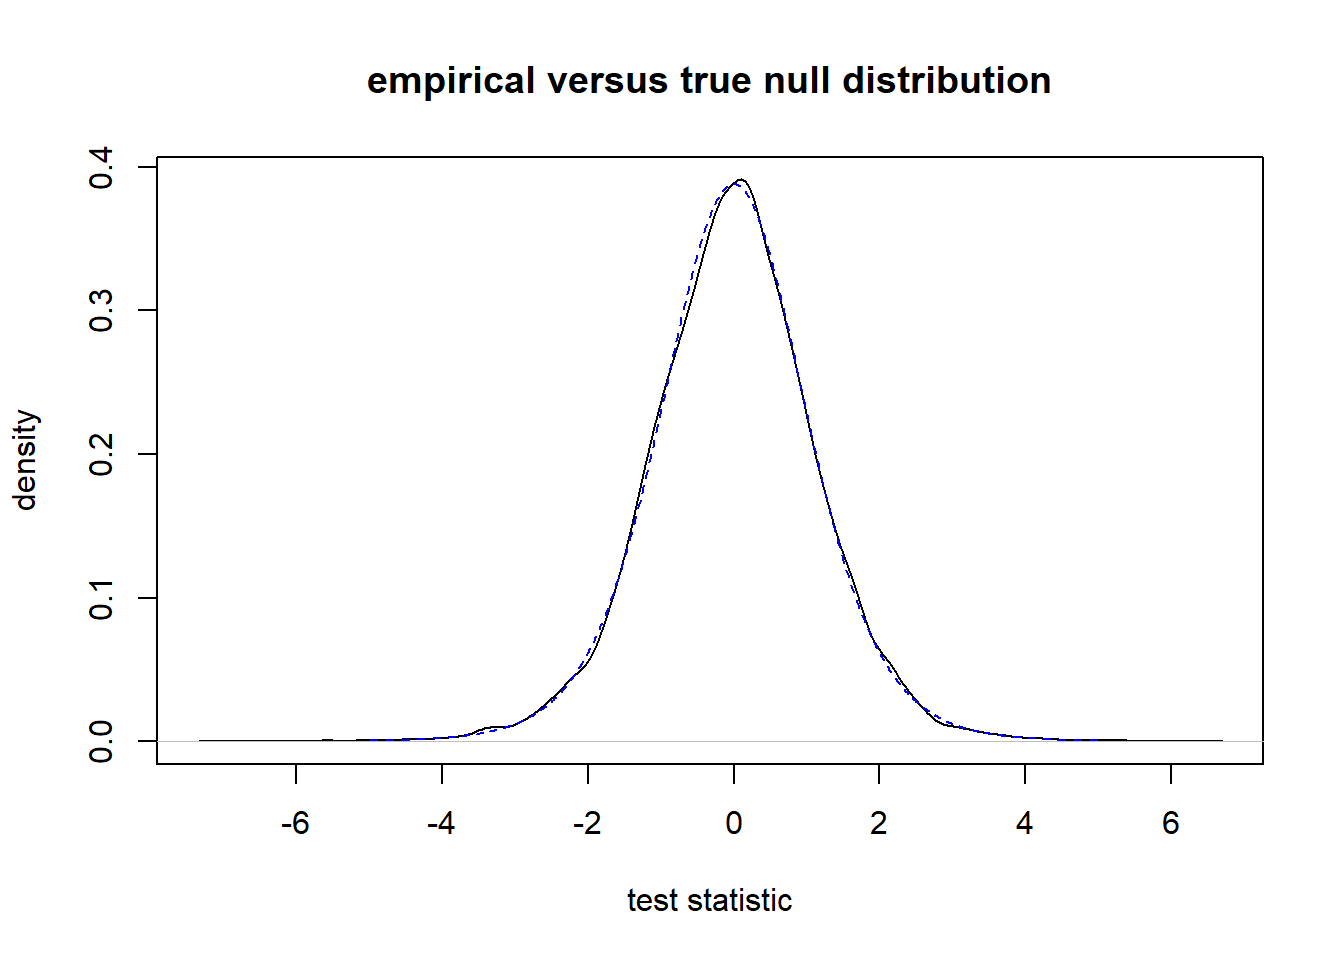
\includegraphics{A-Progessive-Introduction-to-Linear-Models_files/figure-latex/tnullfigure-1.pdf}
\caption{\label{fig:tnullfigure}Comparison of empirical null distribution to theoretical null distribution. The empirical null distribution is shown by the solid black line and the theoretical null distribution by a dashed blue line.}
\end{figure}

What should we takeaway from this example? The null distribution of a hypothesis test is the sampling distribution of the test statistic under the assumption that \(H_0\) is true. We approximated the null distribution of our test statistic by drawing 10,000 samples from the population distribution under the assumption that \(H_0\) was true.

How does the null distribution relate to choosing the rejection region? First, the type I error rate is the probability of rejecting \(H_0\) when \(H_0\) is true. Since we know the null distribution, we know what behavior to expect from our test statistic if \(H_0\) is true. Thus, we know what test statistics are most unlikely if \(H_0\) is true. Let's say we want to control the type I error at \(\alpha = 0.05\). For this upper-tailed test, we should reject \(H_0\) when the test statistic is greater than \(t^{0.05}_9\), i.e., the 0.95 quantile of a \(t\) distribution with 9 degrees of freedom. Why do we use this threshold? Because if \(H_0\) is true, this will only lead to erroneous rejections of \(H_0\) (i.e., a type I error) 5\% of the time. In the code below, we compute the sample proportion of test statistics from our null distribution that are more than \(t^{0.05}_9\). Our sample proportion is very close to 0.05, and this number will converge to 0.05 as we increase the number samples used in our simulation.

\begin{Shaded}
\begin{Highlighting}[]
\FunctionTok{mean}\NormalTok{(tstats }\SpecialCharTok{\textgreater{}} \FunctionTok{qt}\NormalTok{(}\FloatTok{0.95}\NormalTok{, }\AttributeTok{df =} \DecValTok{9}\NormalTok{))}
\DocumentationTok{\#\# [1] 0.0489}
\end{Highlighting}
\end{Shaded}

\hypertarget{confidence-intervals}{%
\section{Confidence Intervals}\label{confidence-intervals}}

A \textbf{confidence interval} provides us with plausible values of a target parameter. It is the most common type of interval estimator.

A confidence interval procedure has an associated \textbf{confidence level}. When independent random samples are taken repeatedly from the population, a confidence interval procedure will produce intervals containing the target parameter with probability equal to the confidence level. Confidence level is associated with a confidence interval \emph{procedure}, not a specific interval. A 95\% confidence interval procedure will produce intervals that contain the target parameter 95\% of the time. A specific interval estimate will either contain the target parameter or it will not.

The formulas for confidence intervals are usually derived from a pivotal quantity. A \textbf{pivotal quantity} is a function of the data and the target parameter whose distribution does not depend on the value of the target
parameter.

\textbf{Example:}

Suppose \(Y_1,Y_2,\ldots,Y_n \stackrel{i.i.d.}{\sim} \mathcal{N}(\mu, 1)\).

The random variable \(Z=(\bar{Y}-\mu)/(1/\sqrt{n})\sim \mathcal{N}(0,1)\) is a pivotal quantity.

Since \(P(-1.96\leq Z\leq 1.96)=0.95\), we can derive that
\[
P(\bar{Y}-1.96\times 1/\sqrt{n}\leq \mu \leq \bar{Y}+1.96\times 1/\sqrt{n})=0.95.
\]

Our 95\% confidence interval for \(\mu\) in this context is
\[
[\bar{Y}-1.96\times 1/\sqrt{n}, \bar{Y}+1.96\times 1/\sqrt{n}].
\]
If \(\bar{Y}=0.551\) and \(n=10\), then the associated 95\% confidence interval for \(\mu\) is {[}-0.070,1.171{]}.

\textbf{More discussion of confidence level}

The CI formula given above is supposed to produce 95\% confidence intervals (i.e., the confidence level of the procedure is 0.95). If produce 100 intervals from independent data sets, then about 95\% of them would contain the true mean, but about 5\% would not. To illustrate this further, we use a small simulation example below to produce 100 95\% confidence intervals using a sample of size n = 10 for a \(\mathcal{N(0,1)}\) population.

First, we obtain 100 samples of size 10 from the population and then compute the sample mean of each sample. We do this in the code below.

\begin{Shaded}
\begin{Highlighting}[]
\CommentTok{\# create matrix to store samples}
\NormalTok{samples }\OtherTok{\textless{}{-}} \FunctionTok{matrix}\NormalTok{(}\DecValTok{0}\NormalTok{, }\AttributeTok{nrow =} \DecValTok{100}\NormalTok{, }\AttributeTok{ncol =} \DecValTok{10}\NormalTok{)}
\CommentTok{\# obtain 100 samples from the population}
\ControlFlowTok{for}\NormalTok{ (i }\ControlFlowTok{in} \DecValTok{1}\SpecialCharTok{:}\DecValTok{100}\NormalTok{) \{}
\NormalTok{  samples[i,] }\OtherTok{\textless{}{-}} \FunctionTok{rnorm}\NormalTok{(}\AttributeTok{n =} \DecValTok{10}\NormalTok{, }\AttributeTok{mean =} \DecValTok{0}\NormalTok{, }\AttributeTok{sd =} \DecValTok{1}\NormalTok{)}
\NormalTok{\}}
\CommentTok{\# calculate the sample mean for each sample}
\NormalTok{means }\OtherTok{=} \FunctionTok{rowMeans}\NormalTok{(samples) }\CommentTok{\#calculates the mean of each row}
\end{Highlighting}
\end{Shaded}

Next, we use the formula above to determine the lower and upper bound of the confidence interval associated with each interval. Since we want 95\% confidence intervals, we use the 0.975 quantile of the standard normal distribution to construct our interval.

\begin{Shaded}
\begin{Highlighting}[]
\CommentTok{\#calculate the lower and upper bounds for the 95\% CIs}
\NormalTok{lb }\OtherTok{=}\NormalTok{ means }\SpecialCharTok{{-}} \FunctionTok{qnorm}\NormalTok{(.}\DecValTok{975}\NormalTok{) }\SpecialCharTok{*} \DecValTok{1}\SpecialCharTok{/}\FunctionTok{sqrt}\NormalTok{(}\DecValTok{10}\NormalTok{)}
\NormalTok{ub }\OtherTok{=}\NormalTok{ means }\SpecialCharTok{+} \FunctionTok{qnorm}\NormalTok{(.}\DecValTok{975}\NormalTok{) }\SpecialCharTok{*} \DecValTok{1}\SpecialCharTok{/}\FunctionTok{sqrt}\NormalTok{(}\DecValTok{10}\NormalTok{)}
\end{Highlighting}
\end{Shaded}

Next, we plot each interval. The intervals are orange if the
interval doesn't contain the true population mean, which is 0. Figure \ref{fig:ci-interp-plot} displays our results.

\begin{Shaded}
\begin{Highlighting}[]
\CommentTok{\#create blank plot}
\FunctionTok{plot}\NormalTok{(}\FunctionTok{range}\NormalTok{(}\FunctionTok{c}\NormalTok{(lb, ub)), }\FunctionTok{c}\NormalTok{(}\DecValTok{1}\NormalTok{,}\DecValTok{100}\NormalTok{),}
     \AttributeTok{xlab =} \StringTok{""}\NormalTok{, }\AttributeTok{ylab =} \StringTok{"interval"}\NormalTok{, }\AttributeTok{type =} \StringTok{"n"}\NormalTok{)}
\CommentTok{\# title plot}
\FunctionTok{title}\NormalTok{(}\StringTok{"Interpretation of a Confidence Interval"}\NormalTok{)}
\CommentTok{\# plot true mean}
\FunctionTok{abline}\NormalTok{(}\AttributeTok{v =} \DecValTok{0}\NormalTok{, }\AttributeTok{col =} \StringTok{"blue"}\NormalTok{)}
\CommentTok{\#plot interval each sample}
\ControlFlowTok{for}\NormalTok{ (i }\ControlFlowTok{in} \DecValTok{1}\SpecialCharTok{:}\DecValTok{100}\NormalTok{) }\FunctionTok{lines}\NormalTok{(}\FunctionTok{c}\NormalTok{(lb[i], ub[i]), }\FunctionTok{c}\NormalTok{(i, i))}
\CommentTok{\#highlight intervals missing 0 in orange}
\ControlFlowTok{for}\NormalTok{ (i }\ControlFlowTok{in} \DecValTok{1}\SpecialCharTok{:}\DecValTok{100}\NormalTok{) \{}
  \ControlFlowTok{if}\NormalTok{ (lb[i] }\SpecialCharTok{\textgreater{}} \DecValTok{0} \SpecialCharTok{|}\NormalTok{ ub[i] }\SpecialCharTok{\textless{}} \DecValTok{0}\NormalTok{ )   \{}
    \FunctionTok{lines}\NormalTok{(}\FunctionTok{c}\NormalTok{(lb[i],ub[i]), }\FunctionTok{c}\NormalTok{(i,i), }\AttributeTok{col =} \StringTok{"orange"}\NormalTok{)}
\NormalTok{  \}}
\NormalTok{\}}
\end{Highlighting}
\end{Shaded}

\begin{figure}
\centering
\includegraphics{A-Progessive-Introduction-to-Linear-Models_files/figure-latex/ci-interp-plot-1.pdf}
\caption{\label{fig:ci-interp-plot}A plot of 100 95\% confidence intervals for a population mean produced from independent samples from a \(\mathcal{N}(0,1)\) population.}
\end{figure}

In this example, 96 out of 100 intervals for the population mean contained the true population mean of 0. Notice how the intervals move around. This is because each sample provides us with slightly different values, so the intervals move around because of the samples obtained. Each interval either contains the true mean of 0 or it does not. But as a whole, the procedure we are using will produce confidence intervals that contain the true mean 95\% of the time.

\hypertarget{linking-hypothesis-tests-and-confidence-intervals}{%
\section{Linking Hypothesis Tests and Confidence Intervals}\label{linking-hypothesis-tests-and-confidence-intervals}}

CIs are directly linked to hypothesis tests.

A \(100(1-\alpha)\%\) two-sided confidence interval for target parameter \(\theta\) is linked with a hypothesis test of \(H_0:\theta = c\) versus \(H_a:\theta \neq c\) tested at level
\(\alpha\).

\begin{itemize}
\tightlist
\item
  Any point that lies within the \(100(1-\alpha)\%\) confidence interval for \(\theta\) represents a value of \(c\) for which the associated null hypothesis would not be rejected at significance level \(\theta\).
\item
  Any point outside of the confidence interval is a value of \(c\) for which the associated null hypothesis would be rejected.
\end{itemize}

Similar relationships hold for one-sided CIs and hypothesis tests.

\textbf{Example:}

Consider the 95\% confidence interval for \(\mu\) we previously
constructed: {[}-0.070,1.171{]}.

That interval is conceptually linked to the statistical test of \(H_0:\mu = c\) versus \(H_a:\mu \neq c\) using \(\alpha =0.05\).

We would reject \(H_0\) for any hypothesized values of \(c\) less than -0.070 or more than 1.171. We would fail to reject \(H_0\) for any values of \(c\) between -0.070 and 1.171.

A confidence interval provides us with much of the same information as a hypothesis test, but it doesn't provide the p-value or allow us to do hypothesis tests at different significance levels.

Confidence intervals are often preferred over hypothesis tests because they provide additional information in the form of plausible parameters values while giving us enough information to perform a hypothesis test.

\hypertarget{references}{%
\chapter*{References}\label{references}}
\addcontentsline{toc}{chapter}{References}

\hypertarget{refs}{}
\begin{CSLReferences}{1}{0}
\leavevmode\vadjust pre{\hypertarget{ref-anscombe1973graphs}{}}%
Anscombe, Francis J. 1973. {``Graphs in Statistical Analysis.''} \emph{The American Statistician} 27 (1): 17--21.

\leavevmode\vadjust pre{\hypertarget{ref-bonferroni1936}{}}%
Bonferroni, Carlo. 1936. {``Teoria Statistica Delle Classi e Calcolo Delle Probabilita.''} \emph{Pubblicazioni Del R Istituto Superiore Di Scienze Economiche e Commericiali Di Firenze} 8: 3--62.

\leavevmode\vadjust pre{\hypertarget{ref-boole}{}}%
Boole, George. 1847. \emph{The Mathematical Analysis of Logic}. Philosophical Library.

\leavevmode\vadjust pre{\hypertarget{ref-boos_stefanski_2011_pvalues}{}}%
Boos, Dennis D., and Leonard A. Stefanski. 2011. {``P-Value Precision and Reproducibility.''} \emph{The American Statistician} 65 (4): 213--21. \url{https://doi.org/10.1198/tas.2011.10129}.

\leavevmode\vadjust pre{\hypertarget{ref-brewer}{}}%
Brewer, Cynthia A. 2022. {``ColorBrewer2.org.''} \url{https://colorbrewer2.org}.

\leavevmode\vadjust pre{\hypertarget{ref-ezekiel1930methods}{}}%
Ezekiel, Mordecai. 1930. {``Methods of Correlation Analysis.''}

\leavevmode\vadjust pre{\hypertarget{ref-lmwr2}{}}%
Faraway, Julian J. 2014. \emph{Linear Models with r}. Second. Chapman; Hall/CRC.

\leavevmode\vadjust pre{\hypertarget{ref-fox2020predictor}{}}%
Fox, John, and Sanford Weisberg. 2020. {``Predictor Effects Graphics Gallery.''} \url{https://cran.r-project.org/web/packages/effects/vignettes/predictor-effects-gallery.pdf}.

\leavevmode\vadjust pre{\hypertarget{ref-R-car}{}}%
Fox, John, Sanford Weisberg, and Brad Price. 2022. \emph{Car: Companion to Applied Regression}. \url{https://CRAN.R-project.org/package=car}.

\leavevmode\vadjust pre{\hypertarget{ref-R-effects}{}}%
Fox, John, Sanford Weisberg, Brad Price, Michael Friendly, and Jangman Hong. 2022. \emph{Effects: Effect Displays for Linear, Generalized Linear, and Other Models}. \url{https://CRAN.R-project.org/package=effects}.

\leavevmode\vadjust pre{\hypertarget{ref-R-api2lm}{}}%
French, Joshua P. 2022. \emph{Api2lm: Functions and Data Sets for the Book "a Progressive Introduction to Linear Models"}. \url{https://CRAN.R-project.org/package=api2lm}.

\leavevmode\vadjust pre{\hypertarget{ref-gibson_pvalue}{}}%
Gibson, Eric W. 2021. {``The Role of p-Values in Judging the Strength of Evidence and Realistic Replication Expectations.''} \emph{Statistics in Biopharmaceutical Research} 13 (1): 6--18. \url{https://doi.org/10.1080/19466315.2020.1724560}.

\leavevmode\vadjust pre{\hypertarget{ref-R-ggiraph}{}}%
Gohel, David, and Panagiotis Skintzos. 2023. \emph{Ggiraph: Make Ggplot2 Graphics Interactive}. \url{https://davidgohel.github.io/ggiraph/}.

\leavevmode\vadjust pre{\hypertarget{ref-GormanEtAl2014}{}}%
Gorman, Kristen B., Tony D. Williams, and William R. Fraser. 2014. {``Ecological Sexual Dimorphism and Environmental Variability Within a Community of Antarctic Penguins (Genus Pygoscelis).''} \emph{PLOS ONE} 9 (3): 1--14. \url{https://doi.org/10.1371/journal.pone.0090081}.

\leavevmode\vadjust pre{\hypertarget{ref-R-palmerpenguins}{}}%
Horst, Allison, Alison Hill, and Kristen Gorman. 2022. \emph{Palmerpenguins: Palmer Archipelago (Antarctica) Penguin Data}. \url{https://CRAN.R-project.org/package=palmerpenguins}.

\leavevmode\vadjust pre{\hypertarget{ref-alsm2005}{}}%
Kutner, Michael H, Christopher J Nachtsheim, John Neter, and William Li. 2005. \emph{Applied Linear Statistical Models, 5th Edition}. McGraw-Hill/Irwin, New York.

\leavevmode\vadjust pre{\hypertarget{ref-bon_vs_scheffe}{}}%
Mi, Jie, and Allan R. Sampson. 1993. {``A Comparison of the Bonferroni and Scheffé Bounds.''} \emph{Journal of Statistical Planning and Inference} 36 (1): 101--5. https://doi.org/\url{https://doi.org/10.1016/0378-3758(93)90105-F}.

\leavevmode\vadjust pre{\hypertarget{ref-mt1977}{}}%
Mosteller, Frederick, and John W Tukey. 1977. \emph{Data Analysis and Regression. A Second Course in Statistics}. \emph{Addison-Wesley, Reading, MA}.

\leavevmode\vadjust pre{\hypertarget{ref-R-tibble}{}}%
Müller, Kirill, and Hadley Wickham. 2023. \emph{Tibble: Simple Data Frames}. \url{https://CRAN.R-project.org/package=tibble}.

\leavevmode\vadjust pre{\hypertarget{ref-R-base}{}}%
R Core Team. 2023. \emph{R: A Language and Environment for Statistical Computing}. Vienna, Austria: R Foundation for Statistical Computing. \url{https://www.R-project.org/}.

\leavevmode\vadjust pre{\hypertarget{ref-sall1990leverage}{}}%
Sall, John. 1990. {``Leverage Plots for General Linear Hypotheses.''} \emph{The American Statistician} 44 (4): 308--15.

\leavevmode\vadjust pre{\hypertarget{ref-sheather2009modern}{}}%
Sheather, Simon. 2009. \emph{A Modern Approach to Regression with r}. Springer, New York.

\leavevmode\vadjust pre{\hypertarget{ref-R-plotly}{}}%
Sievert, Carson, Chris Parmer, Toby Hocking, Scott Chamberlain, Karthik Ram, Marianne Corvellec, and Pedro Despouy. 2022. \emph{Plotly: Create Interactive Web Graphics via Plotly.js}. \url{https://CRAN.R-project.org/package=plotly}.

\leavevmode\vadjust pre{\hypertarget{ref-wasserman2004all}{}}%
Wasserman, Larry. 2004. \emph{All of Statistics: A Concise Course in Statistical Inference}. Vol. 26. Springer.

\leavevmode\vadjust pre{\hypertarget{ref-alr4}{}}%
Weisberg, Sanford. 2014. \emph{Applied Linear Regression}. Fourth. Hoboken {NJ}: Wiley. \url{http://z.umn.edu/alr4ed}.

\leavevmode\vadjust pre{\hypertarget{ref-R-stringr}{}}%
Wickham, Hadley. 2022a. \emph{Stringr: Simple, Consistent Wrappers for Common String Operations}. \url{https://CRAN.R-project.org/package=stringr}.

\leavevmode\vadjust pre{\hypertarget{ref-tidyversestyleguide}{}}%
---------. 2022b. \emph{The Tidyverse Style Guide}. \url{https://style.tidyverse.org/}.

\leavevmode\vadjust pre{\hypertarget{ref-R-forcats}{}}%
---------. 2023a. \emph{Forcats: Tools for Working with Categorical Variables (Factors)}. \url{https://CRAN.R-project.org/package=forcats}.

\leavevmode\vadjust pre{\hypertarget{ref-R-tidyverse}{}}%
---------. 2023b. \emph{Tidyverse: Easily Install and Load the Tidyverse}. \url{https://CRAN.R-project.org/package=tidyverse}.

\leavevmode\vadjust pre{\hypertarget{ref-R-readxl}{}}%
Wickham, Hadley, and Jennifer Bryan. 2023. \emph{Readxl: Read Excel Files}. \url{https://CRAN.R-project.org/package=readxl}.

\leavevmode\vadjust pre{\hypertarget{ref-R-ggplot2}{}}%
Wickham, Hadley, Winston Chang, Lionel Henry, Thomas Lin Pedersen, Kohske Takahashi, Claus Wilke, Kara Woo, Hiroaki Yutani, and Dewey Dunnington. 2023. \emph{Ggplot2: Create Elegant Data Visualisations Using the Grammar of Graphics}. \url{https://CRAN.R-project.org/package=ggplot2}.

\leavevmode\vadjust pre{\hypertarget{ref-R-dplyr}{}}%
Wickham, Hadley, Romain François, Lionel Henry, Kirill Müller, and Davis Vaughan. 2023. \emph{Dplyr: A Grammar of Data Manipulation}. \url{https://CRAN.R-project.org/package=dplyr}.

\leavevmode\vadjust pre{\hypertarget{ref-R-purrr}{}}%
Wickham, Hadley, and Lionel Henry. 2023. \emph{Purrr: Functional Programming Tools}. \url{https://CRAN.R-project.org/package=purrr}.

\leavevmode\vadjust pre{\hypertarget{ref-R-readr}{}}%
Wickham, Hadley, Jim Hester, and Jennifer Bryan. 2023. \emph{Readr: Read Rectangular Text Data}. \url{https://CRAN.R-project.org/package=readr}.

\leavevmode\vadjust pre{\hypertarget{ref-R-tidyr}{}}%
Wickham, Hadley, Davis Vaughan, and Maximilian Girlich. 2023. \emph{Tidyr: Tidy Messy Data}. \url{https://CRAN.R-project.org/package=tidyr}.

\leavevmode\vadjust pre{\hypertarget{ref-wilkinsonrogers1973}{}}%
Wilkinson, GN, and CE Rogers. 1973. {``Symbolic Description of Factorial Models for Analysis of Variance.''} \emph{Journal of the Royal Statistical Society: Series C (Applied Statistics)} 22 (3): 392--99.

\leavevmode\vadjust pre{\hypertarget{ref-workinghotelling}{}}%
Working, Holbrook, and Harold Hotelling. 1929. {``Applications of the Theory of Error to the Interpretation of Trends.''} \emph{Journal of the American Statistical Association} 24 (165A): 73--85. \url{https://doi.org/10.1080/01621459.1929.10506274}.

\leavevmode\vadjust pre{\hypertarget{ref-R-bookdown}{}}%
Xie, Yihui. 2023. \emph{Bookdown: Authoring Books and Technical Documents with r Markdown}. \url{https://CRAN.R-project.org/package=bookdown}.

\leavevmode\vadjust pre{\hypertarget{ref-R-kableExtra}{}}%
Zhu, Hao. 2021. \emph{kableExtra: Construct Complex Table with Kable and Pipe Syntax}. \url{https://CRAN.R-project.org/package=kableExtra}.

\end{CSLReferences}

\end{document}
